% Options for packages loaded elsewhere
\PassOptionsToPackage{unicode}{hyperref}
\PassOptionsToPackage{hyphens}{url}
\documentclass[
  a4paper]{book}
\usepackage{xcolor}
\usepackage{amsmath,amssymb}
\setcounter{secnumdepth}{5}
\usepackage{iftex}
\ifPDFTeX
  \usepackage[T1]{fontenc}
  \usepackage[utf8]{inputenc}
  \usepackage{textcomp} % provide euro and other symbols
\else % if luatex or xetex
  \usepackage{unicode-math} % this also loads fontspec
  \defaultfontfeatures{Scale=MatchLowercase}
  \defaultfontfeatures[\rmfamily]{Ligatures=TeX,Scale=1}
\fi
\usepackage{lmodern}
\ifPDFTeX\else
  % xetex/luatex font selection
\fi
% Use upquote if available, for straight quotes in verbatim environments
\IfFileExists{upquote.sty}{\usepackage{upquote}}{}
\IfFileExists{microtype.sty}{% use microtype if available
  \usepackage[]{microtype}
  \UseMicrotypeSet[protrusion]{basicmath} % disable protrusion for tt fonts
}{}
\makeatletter
\@ifundefined{KOMAClassName}{% if non-KOMA class
  \IfFileExists{parskip.sty}{%
    \usepackage{parskip}
  }{% else
    \setlength{\parindent}{0pt}
    \setlength{\parskip}{6pt plus 2pt minus 1pt}}
}{% if KOMA class
  \KOMAoptions{parskip=half}}
\makeatother
\usepackage{color}
\usepackage{fancyvrb}
\newcommand{\VerbBar}{|}
\newcommand{\VERB}{\Verb[commandchars=\\\{\}]}
\DefineVerbatimEnvironment{Highlighting}{Verbatim}{commandchars=\\\{\}}
% Add ',fontsize=\small' for more characters per line
\usepackage{framed}
\definecolor{shadecolor}{RGB}{248,248,248}
\newenvironment{Shaded}{\begin{snugshade}}{\end{snugshade}}
\newcommand{\AlertTok}[1]{\textcolor[rgb]{0.94,0.16,0.16}{#1}}
\newcommand{\AnnotationTok}[1]{\textcolor[rgb]{0.56,0.35,0.01}{\textbf{\textit{#1}}}}
\newcommand{\AttributeTok}[1]{\textcolor[rgb]{0.13,0.29,0.53}{#1}}
\newcommand{\BaseNTok}[1]{\textcolor[rgb]{0.00,0.00,0.81}{#1}}
\newcommand{\BuiltInTok}[1]{#1}
\newcommand{\CharTok}[1]{\textcolor[rgb]{0.31,0.60,0.02}{#1}}
\newcommand{\CommentTok}[1]{\textcolor[rgb]{0.56,0.35,0.01}{\textit{#1}}}
\newcommand{\CommentVarTok}[1]{\textcolor[rgb]{0.56,0.35,0.01}{\textbf{\textit{#1}}}}
\newcommand{\ConstantTok}[1]{\textcolor[rgb]{0.56,0.35,0.01}{#1}}
\newcommand{\ControlFlowTok}[1]{\textcolor[rgb]{0.13,0.29,0.53}{\textbf{#1}}}
\newcommand{\DataTypeTok}[1]{\textcolor[rgb]{0.13,0.29,0.53}{#1}}
\newcommand{\DecValTok}[1]{\textcolor[rgb]{0.00,0.00,0.81}{#1}}
\newcommand{\DocumentationTok}[1]{\textcolor[rgb]{0.56,0.35,0.01}{\textbf{\textit{#1}}}}
\newcommand{\ErrorTok}[1]{\textcolor[rgb]{0.64,0.00,0.00}{\textbf{#1}}}
\newcommand{\ExtensionTok}[1]{#1}
\newcommand{\FloatTok}[1]{\textcolor[rgb]{0.00,0.00,0.81}{#1}}
\newcommand{\FunctionTok}[1]{\textcolor[rgb]{0.13,0.29,0.53}{\textbf{#1}}}
\newcommand{\ImportTok}[1]{#1}
\newcommand{\InformationTok}[1]{\textcolor[rgb]{0.56,0.35,0.01}{\textbf{\textit{#1}}}}
\newcommand{\KeywordTok}[1]{\textcolor[rgb]{0.13,0.29,0.53}{\textbf{#1}}}
\newcommand{\NormalTok}[1]{#1}
\newcommand{\OperatorTok}[1]{\textcolor[rgb]{0.81,0.36,0.00}{\textbf{#1}}}
\newcommand{\OtherTok}[1]{\textcolor[rgb]{0.56,0.35,0.01}{#1}}
\newcommand{\PreprocessorTok}[1]{\textcolor[rgb]{0.56,0.35,0.01}{\textit{#1}}}
\newcommand{\RegionMarkerTok}[1]{#1}
\newcommand{\SpecialCharTok}[1]{\textcolor[rgb]{0.81,0.36,0.00}{\textbf{#1}}}
\newcommand{\SpecialStringTok}[1]{\textcolor[rgb]{0.31,0.60,0.02}{#1}}
\newcommand{\StringTok}[1]{\textcolor[rgb]{0.31,0.60,0.02}{#1}}
\newcommand{\VariableTok}[1]{\textcolor[rgb]{0.00,0.00,0.00}{#1}}
\newcommand{\VerbatimStringTok}[1]{\textcolor[rgb]{0.31,0.60,0.02}{#1}}
\newcommand{\WarningTok}[1]{\textcolor[rgb]{0.56,0.35,0.01}{\textbf{\textit{#1}}}}
\usepackage{longtable,booktabs,array}
\newcounter{none} % for unnumbered tables
\usepackage{calc} % for calculating minipage widths
% Correct order of tables after \paragraph or \subparagraph
\usepackage{etoolbox}
\makeatletter
\patchcmd\longtable{\par}{\if@noskipsec\mbox{}\fi\par}{}{}
\makeatother
% Allow footnotes in longtable head/foot
\IfFileExists{footnotehyper.sty}{\usepackage{footnotehyper}}{\usepackage{footnote}}
\makesavenoteenv{longtable}
\usepackage{graphicx}
\makeatletter
\newsavebox\pandoc@box
\newcommand*\pandocbounded[1]{% scales image to fit in text height/width
  \sbox\pandoc@box{#1}%
  \Gscale@div\@tempa{\textheight}{\dimexpr\ht\pandoc@box+\dp\pandoc@box\relax}%
  \Gscale@div\@tempb{\linewidth}{\wd\pandoc@box}%
  \ifdim\@tempb\p@<\@tempa\p@\let\@tempa\@tempb\fi% select the smaller of both
  \ifdim\@tempa\p@<\p@\scalebox{\@tempa}{\usebox\pandoc@box}%
  \else\usebox{\pandoc@box}%
  \fi%
}
% Set default figure placement to htbp
\def\fps@figure{htbp}
\makeatother
\setlength{\emergencystretch}{3em} % prevent overfull lines
\providecommand{\tightlist}{%
  \setlength{\itemsep}{0pt}\setlength{\parskip}{0pt}}
\usepackage[]{natbib}
\bibliographystyle{apalike}
\usepackage{booktabs}
\usepackage{tcolorbox}
\usepackage[a4paper,margin=2.5cm]{geometry}

\setlength{\fboxsep}{.8em}

\newtcolorbox{do-something}{
  colback=black!10!white,
  colframe=orange,
  coltext=black,
  boxsep=5pt,
  arc=4pt}

% \lstset{
%  breaklines=true
% }


% Don't load hyperref yourself; let Pandoc handle it.
% Just override its setup *after* Pandoc has loaded it.
\AtBeginDocument{%
  \hypersetup{
    colorlinks=true,
    linkcolor=black,    % internal TOC & cross-refs
    urlcolor=blue,      % external URLs
    citecolor=darkgray  % citations
  }%
}
\usepackage{bookmark}
\IfFileExists{xurl.sty}{\usepackage{xurl}}{} % add URL line breaks if available
\urlstyle{same}
% fallback for those not using the hyperref driver hyperxmp:
\makeatletter
\@ifundefined{xmpquote}{\newcommand{\xmpquote}[1]{#1}}{}
\makeatother
\hypersetup{
  pdftitle={BB512 - Population Biology and Evolution},
  pdfauthor={Owen R. Jones (Course Coordinator)},
  hidelinks,
  pdfcreator={LaTeX via pandoc}}

\title{BB512 - Population Biology and Evolution}
\author{Owen R. Jones (Course Coordinator)}
\date{2026-10-28}

\begin{document}
\maketitle

{
\setcounter{tocdepth}{1}
\tableofcontents
}
\chapter{Welcome to BB512}\label{welcome-to-bb512}

Welcome to the Population and Evolution course.
The course, and this website, is divided into five parts:

\begin{enumerate}
\def\labelenumi{\arabic{enumi}.}
\tightlist
\item
  Evolution by Natural Selection
\item
  Population Growth Models
\item
  Population Genetics and Evolution
\item
  Interactions Between Species and Community Structure
\item
  Animal Behaviour, Altruism and Sexual Selection
\end{enumerate}

The recommended textbook is Neal (2018). Other useful textbooks, that are NOT mandatory, but could be useful are Gotelli (2008) and Stearns \& Hoekstra (2005).

\begin{itemize}
\tightlist
\item
  Neal, D. (2018). \emph{Introduction to Population Biology} (2nd edition). Cambridge: Cambridge University Press. \url{doi:10.1017/9781139107976}
\item
  Gotelli, NJ (2008) \emph{A Primer of Ecology}. Fourth Edition, Sinauer Associates. ISBN: 978-0878933181
\item
  Stearns, SC \& Hoekstra, RF (2005) \emph{Evolution: An Introduction}. 2nd Edition, Oxford University Press. ISBN: 978-0199255634
\end{itemize}

In addition to this, I will provide a reading list of journal articles that are relevant to the material. These are optional, but highly recommended because they give extra context and background to the course and show you how the theory is used in recent research.

\section{How to use this book}\label{how-to-use-this-book}

Each chapter follows a consistent template so you can move quickly between concepts and tasks.

\begin{itemize}
\tightlist
\item
  Learning outcomes: what you should be able to do by the end.
\item
  Background: the core concepts and equations.
\item
  Worked example: a short walk-through that shows the method.
\item
  Your task: the practical exercise or analysis.
\item
  Takeaways: a short summary of the main ideas.
\end{itemize}

If you are short on time, read the Learning outcomes and Takeaways first, then do the Your task section. Use the worked example only if you need a refresher.

\section{Parts overview}\label{parts-overview}

The table below shows how each part maps onto the major skills you will build through the course.

{\def\LTcaptype{none} % do not increment counter
\begin{longtable}[]{@{}
  >{\raggedright\arraybackslash}p{(\linewidth - 4\tabcolsep) * \real{0.3333}}
  >{\raggedright\arraybackslash}p{(\linewidth - 4\tabcolsep) * \real{0.3333}}
  >{\raggedright\arraybackslash}p{(\linewidth - 4\tabcolsep) * \real{0.3333}}@{}}
\toprule\noalign{}
\begin{minipage}[b]{\linewidth}\raggedright
Part
\end{minipage} & \begin{minipage}[b]{\linewidth}\raggedright
Focus
\end{minipage} & \begin{minipage}[b]{\linewidth}\raggedright
Skills you build
\end{minipage} \\
\midrule\noalign{}
\endhead
\bottomrule\noalign{}
\endlastfoot
1. Evolution by Natural Selection & Selection, adaptation, variation & Explain selection in natural contexts; identify selective pressures and outcomes \\
2. Population Growth Models & Exponential and logistic growth, stochasticity & Build and interpret population growth models; reason about parameter effects \\
3. Population Genetics and Evolution & Allele frequencies, drift, heritability & Analyze genetic change over time; estimate heritability from data \\
4. Interactions Between Species and Community Structure & Competition and predator-prey models & Evaluate stability and dynamics of interacting species \\
5. Animal Behaviour, Altruism and Sexual Selection & Game theory and behavior & Interpret behavior through evolutionary payoffs and strategies \\
6. Solutions/answers & Answer keys and model results & Check work and compare interpretations \\
7. Appendix - extras & Extensions and advanced examples & Apply methods to additional contexts \\
\end{longtable}
}

\section{This website and other course materials}\label{this-website-and-other-course-materials}

This website holds most of the materials you need for the practical exercises you will do during the course. You will also find the \href{https://jonesor.github.io/BB512_Book/schedule.html}{Schedule here} (on the web-version only).

\textbf{We may not do ALL of these exercises, but you are welcome to do ones we miss in your own time.}

You will find other materials via itsLearning.

For most classes you will need your personal laptops: Please bring them to class (and remember a power supply!).

\section{Expectations}\label{expectations}

There are lectures and practical exercise sessions on the course. The practical sessions are designed to help you understand the subject better and I expect students to attend and actively participate in both. There will also be some multiple-choice quizzes (e-tests) during the semester. These are intended to help you figure out whether you know the material, and whether there are areas you need to revisit. They do not contribute to your final grade, but I hope you will attempt them. They will definitely increase your understanding of the material. Note that the final assessment will be a similar format!

I expect students to make every effort to keep up with the core reading (mainly the textbook chapters), and to ask questions where they don't understand.

\section{Assessment}\label{assessment}

The assessment for the course will be an electronic exam held in January with multiple-choice and short answer questions. It is worth noting that exam format will be similar to the quizzes mentioned above. The date for the exam will be finalised in December.

\section{Instructors}\label{instructors}

The instructors of the course are:

\begin{itemize}
\tightlist
\item
  \href{https://portal.findresearcher.sdu.dk/en/persons/jones}{Owen Jones}, Associate Professor, \href{mailto:jones@biology.sdu.dk}{\nolinkurl{jones@biology.sdu.dk}}
\item
  \href{https://portal.findresearcher.sdu.dk/en/persons/thomasbb}{Thomas Bjørneboe Berg}, Associate Prof./Senior Scientist at Naturama, \href{mailto:thomas@naturama.dk}{\nolinkurl{thomas@naturama.dk}}
  NULL
\end{itemize}

If you have any problems accessing materials, or have any questions regarding the course feel free to send me (Owen) an email, or make a comment in the form I mentioned above. You can also make an appointment to see me via Zoom or in my office if necessary*. PLEASE REMEMBER to tell me which course you are referring to if you send an email!

Owen Jones, course coordinator - \href{mailto:jones@biology.sdu.dk}{\nolinkurl{jones@biology.sdu.dk}}

Office location: \href{https://clients.mapsindoors.com/sdu/573f26e4bc1f571b08094312/details/563cb94f423b7d0540c9a605}{V12-410b-2}

\section{Software}\label{software}

We will use Excel and R/RStudio during this course.

\subsection{Excel}\label{excel}

I expect you will already have Excel installed, so there is not much to say here.

Be aware that Excel differs depending on the language it is localised in. For example, Danish vs.~English. This means that some of the commands might differ between versions.
See \href{https://easy-excel.com/excel-in-other-languages/excel-formulas-in-danish/}{here} for examples.

\subsection{R and RStudio}\label{r-and-rstudio}

R and RStudio are two separate pieces of software. RStudio is a user-friendly interface to talk to R, it cannot work if you have not got R installed. So, when you install these two programs, install R first, then RStudio.

Already have them installed? I strongly recommend updating to the latest versions of R and RStudio, which you can download at the following sites:

\begin{itemize}
\tightlist
\item
  R: \url{https://cran.r-project.org}
\item
  RStudio: \url{https://www.rstudio.com/products/rstudio/}.
\end{itemize}

If you are unsure whether you should update your R or RStudio try the following code. If it produces a nice graph, then your R is sufficiently up-to-date. If there are error messages, then you probably need to update R.

\begin{verbatim}
install.packages("popdemo")
library(popdemo)

A <- matrix(c(0,1,2,0.5,0.1,0,0,0.6,0.6), byrow=TRUE, ncol=3)

pr <- project(A, vector="n", time=10)
plot(pr)
\end{verbatim}

\textbf{This book includes equations.}

Equations sometimes do not render correctly on some web browsers.

From experience, Chrome tends to be the most reliable, Safari (Mac only) also works well.

Can you see the following equation?

\(N_{t+1}=N_{t}+r_{m} N_{t}\left(1-\frac{N_{t}}{K}\right)\)

It should look like this:

\pandocbounded{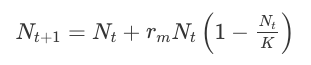
\includegraphics[keepaspectratio]{BB512_files/testEquation.png}}

If it doesn't look right, then you should try another browser (maybe even your phone browser) or investigate a solution.

\section{Schedule}\label{schedule}

The formatted schedule table appears only in the online version of this book.

\begin{itemize}
\tightlist
\item
  View the live schedule page: \url{https://jonesor.github.io/BB512_Book/schedule.html}
\item
  Official SDU timetable (always up to date): \url{https://mitsdu.sdu.dk/skema/activity/N100007101/e26}
\item
  For dates, times and rooms, also check itsLearning.
\end{itemize}

\chapter*{Part 1: Evolution by Natural Selection}\label{part-1}
\addcontentsline{toc}{chapter}{Part 1: Evolution by Natural Selection}

This part introduces the core logic of natural selection using simple, concrete activities. You will move from a conceptual model of selection to an interactive simulation of adaptation.

By the end of Part 1, you should be able to:

\begin{itemize}
\tightlist
\item
  Explain how selection can generate order from random variation.
\item
  Identify the roles of variation, heritability, and environment in adaptation.
\item
  Describe how selection pressures shape trait distributions over time.
\end{itemize}

\chapter{The Blind Watchmaker}\label{the-blind-watchmaker}

\section{Background}\label{background}

\emph{If a pocket watch is found on a heath, it is most reasonable to assume that someone dropped it and that it was made by at least one watchmaker, not by natural forces.}

This is the ``watchmaker analogy'', made famous by the theologian William Paley in his book \emph{Natural Theology} (1802), more than 50 years before Darwin published \emph{On the Origin of Species}. Paley argued that, just as finding a pocket watch would naturally lead one to infer a skilled watchmaker, the intricate structures and adaptations of living organisms (such as the eye) must also imply the existence of an intelligent designer. Darwin read Paley as a student at Cambridge and admired the argument; his theory of natural selection was, in part, an answer to it.

More than a century later, the evolutionary biologist Richard Dawkins took up the same image in his 1986 book \emph{The Blind Watchmaker}. Dawkins argued that the complexity and diversity of life can arise through a ``blind'' process, natural selection, which is unguided and has no foresight. Evolution, like a blind watchmaker, can achieve impressive complexity through small, incremental changes selected over long periods of time.

\subsection{Randomness and Selection}\label{randomness-and-selection}

In this exercise, we will explore how random variation, when paired with selection, can lead to outcomes that would otherwise seem impossible. We will use an R program to simulate the typing of a target sentence through random letter generation. This is a simplified version of a famous computer program described by Dawkins, who used the target phrase ``METHINKS IT IS LIKE A WEASEL'' (a line from Shakespeare's \emph{Hamlet}).

The key idea is the difference between two kinds of selection that Dawkins described:

\begin{itemize}
\tightlist
\item
  \textbf{Single-step selection:} the whole phrase is produced at random in one go, and kept only if it is completely right. Every attempt starts again from scratch.
\item
  \textbf{Cumulative selection:} each generation starts from the previous one, and improvements are kept and built on.
\end{itemize}

By simulating this process, you will discover how random changes alone produce nonsense, but random changes combined with cumulative selection quickly reach the target.

\section{Learning outcomes}\label{learning-outcomes}

Learning outcomes:

\begin{itemize}
\tightlist
\item
  Gain a deeper understanding of adaptive evolution via natural selection.
\item
  Explain the difference between single-step and cumulative selection.
\item
  Recognise how random change can lead to order if paired with selection.
\item
  Run and modify a simple R simulation to explore a biological idea.
\end{itemize}

\section{Worked example}\label{worked-example}

\subsection{Inputs}\label{inputs}

Imagine you are typing random letters on a typewriter. How long would it take to type a sensible sentence by pure chance? Take Dawkins' phrase ``\texttt{METHINKS\ IT\ IS\ LIKE\ A\ WEASEL}'' (28 characters, including spaces).

\subsection{Steps}\label{steps}

The R code below picks each character at random from the 26 letters of the alphabet plus a space, giving a pool of 27 possible characters at each position. The chance of randomly typing the first letter correctly is 1 in 27. The probability of getting the first two letters right is \((1/27)^2\), and the chance of typing the entire 28-character phrase correctly in one attempt is \((1/27)^{28} \approx 8 \times 10^{-41}\). On average you would need about \(27^{28} \approx 1.2 \times 10^{40}\) attempts. This is single-step selection, and it would never work in practice.

\subsection{Output and interpretation}\label{output-and-interpretation}

But what if every correct letter was kept, and only the wrong ones were typed again in the next generation? That is cumulative selection. Let's find out how much difference it makes.

\section{Your task}\label{your-task}

\begin{enumerate}
\def\labelenumi{\arabic{enumi}.}
\setcounter{enumi}{-1}
\tightlist
\item
  Make sure you have both R and RStudio installed.
\item
  Open RStudio.
\item
  Open a new script (File \textgreater{} New File \textgreater{} New Script)
\item
  Copy and paste the R code (below) into your script.
\item
  Save your script with a memorable file name.
\end{enumerate}

Note: only edit the top part of the code (above the line of \texttt{\#} symbols). The phrase can only contain letters and spaces.

\textbf{Predict first}

Before you run the code, write down your predictions:

\begin{itemize}
\tightlist
\item
  With selection turned on, roughly how many generations will it take to reach the target phrase? 10? 100? 10,000?
\item
  With selection turned off, will it ever get there?
\end{itemize}

\subsection{The code}\label{the-code}

\begin{Shaded}
\begin{Highlighting}[]
\NormalTok{phrase }\OtherTok{\textless{}{-}} \StringTok{"Methinks it is like a weasel"}
\NormalTok{nGenerations }\OtherTok{\textless{}{-}} \DecValTok{200}
\NormalTok{selection }\OtherTok{\textless{}{-}} \ConstantTok{TRUE}

\DocumentationTok{\#\#\#\#\#\#\#\#\#\#\#\#\#\#\#\#\#\#\#\#\#\#\#\#\#\#\#\#\#\#\#\#\#\#\#\#\#\#\#\#\#\#\#\#\#\#\#\#\#\#\#}
\CommentTok{\# Do not edit below this line}
\NormalTok{pool }\OtherTok{\textless{}{-}} \FunctionTok{c}\NormalTok{(LETTERS, }\StringTok{" "}\NormalTok{)}
\NormalTok{phraseSplit }\OtherTok{\textless{}{-}} \FunctionTok{unlist}\NormalTok{(}\FunctionTok{strsplit}\NormalTok{(}\FunctionTok{toupper}\NormalTok{(phrase), }\StringTok{""}\NormalTok{))}
\ControlFlowTok{if}\NormalTok{ (}\SpecialCharTok{!}\FunctionTok{all}\NormalTok{(phraseSplit }\SpecialCharTok{\%in\%}\NormalTok{ pool)) }\FunctionTok{stop}\NormalTok{(}\StringTok{"Use only letters and spaces in the phrase"}\NormalTok{)}
\NormalTok{output }\OtherTok{\textless{}{-}} \FunctionTok{data.frame}\NormalTok{(}\AttributeTok{generation =} \DecValTok{1}\SpecialCharTok{:}\NormalTok{nGenerations, }
                     \AttributeTok{phrase =} \FunctionTok{rep}\NormalTok{(}\ConstantTok{NA}\NormalTok{, nGenerations))}
\NormalTok{fixed }\OtherTok{\textless{}{-}} \ConstantTok{NULL}
\ControlFlowTok{for}\NormalTok{ (i }\ControlFlowTok{in} \DecValTok{1}\SpecialCharTok{:}\NormalTok{nGenerations)\{}
\NormalTok{  randomPhrase }\OtherTok{\textless{}{-}} \FunctionTok{sample}\NormalTok{(pool, }\FunctionTok{length}\NormalTok{(phraseSplit), }\AttributeTok{replace =} \ConstantTok{TRUE}\NormalTok{)}
  \ControlFlowTok{if}\NormalTok{(selection }\SpecialCharTok{==} \ConstantTok{TRUE}\NormalTok{) \{}
\NormalTok{    randomPhrase[fixed] }\OtherTok{\textless{}{-}}\NormalTok{ phraseSplit[fixed]}
\NormalTok{    fixed }\OtherTok{\textless{}{-}} \FunctionTok{append}\NormalTok{(fixed, }\FunctionTok{which}\NormalTok{(randomPhrase }\SpecialCharTok{==}\NormalTok{ phraseSplit))}
\NormalTok{    fixed }\OtherTok{\textless{}{-}} \FunctionTok{sort}\NormalTok{(}\FunctionTok{unique}\NormalTok{(fixed))}
\NormalTok{  \}}
\NormalTok{  output}\SpecialCharTok{$}\NormalTok{phrase[i] }\OtherTok{\textless{}{-}} \FunctionTok{paste}\NormalTok{(randomPhrase, }\AttributeTok{collapse =} \StringTok{""}\NormalTok{)}
\NormalTok{\}}
\DocumentationTok{\#\#\#\#\#\#\#\#\#\#\#\#\#\#\#\#\#\#\#\#\#\#\#\#\#\#\#\#\#\#\#\#\#\#\#\#\#\#\#\#\#\#\#\#\#\#\#\#\#\#\#}

\NormalTok{output}

\CommentTok{\# First generation that matches the target (NA if it was never reached)}
\FunctionTok{which}\NormalTok{(output}\SpecialCharTok{$}\NormalTok{phrase }\SpecialCharTok{==} \FunctionTok{paste}\NormalTok{(phraseSplit, }\AttributeTok{collapse =} \StringTok{""}\NormalTok{))[}\DecValTok{1}\NormalTok{]}
\end{Highlighting}
\end{Shaded}

\section{How the simulation works}\label{how-the-simulation-works}

An instructor will explain the code and demonstrate its use.

The program generates a random sequence of characters of the same length as the target phrase (stored in \texttt{phrase}). If selection is turned on (\texttt{selection\ \textless{}-\ TRUE}), correct letters are ``fixed'' in place and kept in every following generation, while incorrect letters continue to be replaced at random. This is cumulative selection: each generation builds on the one before.

Over the generations, the number of correct letters builds up until the sequence matches the target phrase. The last line of the code tells you the generation at which this happened. With selection turned off, each generation is a fresh random guess (single-step selection), and no meaningful sentence appears.

Note that this program is a simplified version of Dawkins' original. Here, each correct letter is locked in place and can never change again. Dawkins' program instead made a population of copies of the current phrase, each with a few random copying errors (mutations), and kept the copy closest to the target. In that version a correct letter can, in principle, be lost again, as in real populations. Both versions show the same thing: cumulative selection is enormously faster than chance alone.

\textbf{Try it yourself}

\begin{enumerate}
\def\labelenumi{\arabic{enumi})}
\tightlist
\item
  \textbf{Change the phrase}: make it shorter or longer (letters and spaces only). How does this change the number of generations needed?
\item
  \textbf{Change the number of generations}: experiment with different values for \texttt{nGenerations}. With 100 generations, is the target always reached?
\item
  \textbf{Repeat the simulation}: run the code again with the same settings. Does it always take the same number of generations?
\item
  \textbf{Turn selection off}: set \texttt{selection\ \textless{}-\ FALSE}. What happens?
\end{enumerate}

\section{Questions}\label{questions}

\begin{itemize}
\tightlist
\item
  What happens if selection is turned OFF?
\item
  Does the number of generations affect whether the target phrase is reached?
\item
  Does the speed of reaching the target phrase depend on the length of the phrase?
\item
  How does this simulation differ from real natural selection?
\end{itemize}

\section{Takeaways}\label{takeaways}

\begin{itemize}
\tightlist
\item
  Cumulative selection, which keeps and builds on small random improvements, is enormously faster than single-step selection (pure chance).
\item
  Random variation alone is extremely unlikely to generate complex outcomes, but selection changes the odds.
\item
  Real natural selection has no target; it favours traits that improve fitness in the current environment.
\end{itemize}

\chapter{Bug hunt camouflage (NetLogo)}\label{bug-hunt-camouflage-netlogo}

\section{Background}\label{background-1}

Adaptive evolution via natural selection is a fundamental concept in evolutionary biology and is one of the central mechanisms driving the diversity of life on Earth. This process is shaped by the interplay between variation in heritable traits within a population, differential survival and reproduction rates, and the environmental challenges faced by organisms. One illustrative example of natural selection is the phenomenon of camouflage in predator-prey systems.

In an environment where predators rely on visual cues to locate their prey, individuals with better camouflage that matches their surroundings are more likely to avoid detection and capture, leading to higher survival rates. Over generations, the frequency of camouflage traits increases in the prey population due to higher survival and increased reproduction of well-camouflaged individuals.

On the other hand, predators with better detection skills, like keen eyesight, are more successful at capturing prey, leading to increased survival and reproduction of these individuals. Consequently, traits associated with effective predation also become more prevalent in the predator population. This dynamic interplay between camouflage in prey and predator detection abilities exemplifies the power of natural selection in driving the adaptation and evolution of species to their ecological niches.

\section{Learning outcomes}\label{learning-outcomes-1}

Learning outcomes:

\begin{itemize}
\tightlist
\item
  Understand adaptive evolution via natural selection.
\item
  Identify the four conditions for evolution by natural selection in a model.
\item
  Explain how fitness depends on the environment.
\item
  Use the terms adaptation, selection, selection pressure, and heritability correctly.
\end{itemize}

\section{Your task}\label{your-task-1}

In this exercise, you will use an individual-based simulation to examine adaptive evolution and natural selection, exploring how living organisms can undergo transformations to better survive and thrive in their environments. You step into the role of a predatory bird and hunt bugs living in a virtual landscape. You will see how the colours of the bugs (``traits'') influence their survival. The bugs that blend into their surroundings have a higher chance of avoiding detection, leading to greater survival and more opportunities to pass on their advantageous traits to future generations.

The exercise is done using one of the built-in models in a computer program called NetLogo (\url{https://ccl.northwestern.edu/netlogo/}).

There are two ways to use NetLogo: (1) You can log in to our SDU UCloud computing system at \url{https://cloud.sdu.dk/}, and use it there; (2) You can download and install NetLogo from the site above.

I recommend the UCloud option: Please follow these steps: (i) search for NetLogo in the search bar at the top of the screen; (ii) click on Applications and then on the NetLogo icon; (iii) click on ``Run Application''; (iv) Give your job a name (e.g., ``BB512'') and under ``Hours'' enter 1 hour; (v) under Machine Type, select ``u1-standard-1''; (vi) click on Submit. After a few moments while UCloud is preparing your job, a new screen appears. Click on Open Interface to open a virtual desktop. There, you can open NetLogo and use it as if it was on your own computer by clicking on its icon.

Open NetLogo and click File \textgreater{} Models Library. You can then use the search box at the bottom of the screen to find the model called ``Bug Hunt Camouflage''.

This is a model of natural/artificial selection that shows how a population hunted by a predator can develop camouflaging. For example, in a forest with green leaves, green bugs may emerge as the predominant bug colour.

In the simulation you assume the role of a predatory bird that feeds on insects, which can be different colours. You will see what effect your hunting has on the colour traits/genetics of these simulated insects, and also how this evolution affects your hunting efficiency.

\subsection{How the simulation works}\label{how-the-simulation-works-1}

Read this before you start, so that you know what the model does (and does not) include.

The simulation starts with bugs of random colours. Each bug has three pigment ``genes'' (red, green and blue) that together set its colour (see ``Details about colours'' at the end).

The model makes these assumptions:

\begin{itemize}
\tightlist
\item
  \textbf{Constant population size.} Each time you catch a bug, one of the surviving bugs is chosen at random to produce one offspring, so the number of bugs stays at the carrying capacity.
\item
  \textbf{Asexual reproduction.} An offspring has a single parent and inherits its colour genes.
\item
  \textbf{Small mutations.} Each of the offspring's three colour genes can differ slightly from the parent's, by up to the value of the ``max-mutation-step'' slider.
\item
  \textbf{Offspring appear near their parent}, within the distance set by the ``offspring-distance'' slider.
\item
  \textbf{Newborn bugs start very small} and grow to full size over time.
\item
  \textbf{Bugs do not move}, and the predator (you) is the only cause of death.
\end{itemize}

So if you consistently catch (e.g.) non-reddish bugs, the reddish bugs that remain will have offspring that are also reddish, and the average colour of the population will shift towards red.

Evolution can be defined as: ``\emph{change in the heritable characteristics {[}colour traits{]} of biological populations {[}bugs{]} over successive generations {[}time{]}.}''

\subsection{Predict first}\label{predict-first}

Before you run the model, write down your predictions:

\begin{enumerate}
\def\labelenumi{\arabic{enumi}.}
\tightlist
\item
  What will happen to the average colour of the bugs after you have hunted for two minutes on one background?
\item
  What will happen to the time it takes you to catch 10 bugs?
\item
  What will happen when you then switch to a different background?
\end{enumerate}

You will check these predictions against what you observe.

\subsection{Getting started}\label{getting-started}

\begin{enumerate}
\def\labelenumi{\arabic{enumi}.}
\tightlist
\item
  When you open the model, you will see a screen with various purple and green ``sliders'', buttons and menus that control parts of the model.
\item
  Start with 30 bugs, by moving the ``carrying-capacity'' slider until it reads 30.
\item
  Now click ``setup''. You should see the environment appear on the right hand side, and you should see a few ``bugs'' on the environment. Start the simulation by clicking ``go''.
\item
  After you click go, you need to click on bugs as fast as you can using your mouse/track pad. You can also keep the mouse button depressed, and move the cursor around the world to catch the bugs. Try to consume bugs as fast as possible to remove any ``deliberation'' on your part as a predator. The camouflaging effect will emerge more clearly if you aren't taking your time trying to find bugs that typically would be more difficult to find.
\end{enumerate}

You can track your progress by looking at the graphs on the left. The most useful are (1) the number of bugs caught through time, (2) the time taken to catch each batch of 10 bugs, and (3) the average colour values of the bugs.

In the ``Bugs Caught vs.~Time'' plot the slope of the curve gives a good idea of your hunting efficiency: the faster you can catch bugs, the steeper the slope. If you didn't catch any bugs for a while, the slope would be horizontal.

You should notice that bugs with contrasting colours (e.g.~black on white) are easier to catch. Keep hunting for 2 minutes, then pause the simulation by clicking ``go'' again. Now take a look at the graphs and see what effect your hunting has had on the colours in the population.

\subsection{Measure your hunting efficiency}\label{measure-your-hunting-efficiency}

Use the ``Time to catch 10 bugs'' plot to put numbers on your hunting efficiency. Record:

{\def\LTcaptype{none} % do not increment counter
\begin{longtable}[]{@{}ll@{}}
\toprule\noalign{}
& Time to catch 10 bugs \\
\midrule\noalign{}
\endhead
\bottomrule\noalign{}
\endlastfoot
First 10 bugs & \\
Last 10 bugs before you switch background & \\
First 10 bugs after you switch background & \\
Last 10 bugs on the new background & \\
\end{longtable}
}

Compare your numbers with your neighbour's. They will differ (you are different predators!), but is the pattern the same?

\section{Questions}\label{questions-1}

Answer the following questions, then make sure you confirm your understanding and have the right answers with an instructor.

\begin{itemize}
\tightlist
\item
  What happens to the average colour of the bug population with time as you hunt? Was your prediction correct?
\item
  What happens to your hunting efficiency? Use your measurements.
\item
  Would you say that the bug population becomes worse or better adapted to their environment?
\item
  Can you explain how this happens?
\item
  After simulating in one environment (e.g.~poppy field) for a few minutes, pause then switch to another environment. Are the bugs now well- or poorly-adapted to their environment?
\item
  Do the genotypes of individuals change (e.g.~with individual age)?
\item
  Increasing the ``max-mutation-step'' makes bug offspring less like their parents. How do you think this will influence the speed of adaptation of the bugs?
\item
  In the lecture we met four conditions for evolution by natural selection: (1) individuals vary in a trait, (2) individuals vary in reproductive success, (3) the trait affects reproductive success, and (4) the trait is inherited. Where do you see each of these in the model? Where does new variation come from?
\item
  Newborn bugs start very small. Could this let some bugs escape for reasons that have nothing to do with their colour? How might that affect the results?
\item
  How does this model differ from a real predator--prey system? Give at least two differences.
\end{itemize}

Some useful keywords:

\begin{itemize}
\tightlist
\item
  Selection
\item
  Adaptation
\item
  Selection pressure
\item
  Heritability
\end{itemize}

\textbf{Optional extension: gene flow and local adaptation}

In the lecture we saw that gene flow can swamp local adaptation. You can explore this with the ``offspring-distance'' slider, which sets how far from its parent an offspring can appear.

\begin{enumerate}
\def\labelenumi{\arabic{enumi}.}
\tightlist
\item
  Choose the background with the most distinct patches of different colour.
\item
  Set ``offspring-distance'' to a small value and hunt for a few minutes. Use ``flash'' or ``clear-background'' to see where the bugs are. Do bugs in different patches come to match their own patch?
\item
  Repeat with a large ``offspring-distance''. What happens now, and why?
\end{enumerate}

\section{Details about colours (optional)}\label{details-about-colours-optional}

Each bug has three pigment genes: red, green and blue. Each gene has a value from 0 to 100, which sets how strongly that pigment is expressed. Switch on ``show-genotype?'' to see each bug's values; for example, 40-100-24 means red at 40\%, green at 100\% and blue at 24\%. The three pigments are mixed, as in the pixels of a TV or computer screen, to give the bug's colour. A bug with a lot of red but little green or blue looks red.

The plots summarise colour in a different way, as \textbf{hue}, \textbf{saturation} and \textbf{brightness} (Fig \ref{fig:colours}):

\begin{itemize}
\tightlist
\item
  \textbf{Hue} is the position around the colour wheel: red, through orange, yellow, green and blue, and back to red.
\item
  \textbf{Saturation} is how vivid the colour is. Low saturation gives washed-out colours (greys, and white at full brightness).
\item
  \textbf{Brightness} is how light or dark the colour is. A brightness of 0 is black, whatever the hue.
\end{itemize}

\begin{figure}

{\centering 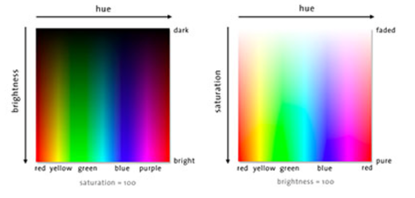
\includegraphics[width=0.65\linewidth]{images/colours} 

}

\caption{Hue, brightness and saturation}\label{fig:colours}
\end{figure}

If this figure does not display in your browser, open it directly here: \href{images/colours.png}{Hue, brightness and saturation diagram}.

Read more about the model here: \url{http://ccl.northwestern.edu/netlogo/models/BugHuntCamouflage}

\section{Takeaways}\label{takeaways-1}

\begin{itemize}
\tightlist
\item
  Selection changes trait distributions when survival depends on the environment.
\item
  All four conditions for evolution by natural selection are present in the model; mutation supplies the new variation.
\item
  Adaptation is context-dependent: a well-adapted population can become poorly adapted when conditions change.
\item
  Heritability and mutation govern how quickly populations can respond to selection pressure.
\end{itemize}

\chapter*{Part 2: Population Growth Models}\label{part-2}
\addcontentsline{toc}{chapter}{Part 2: Population Growth Models}

This part builds the core toolkit for describing and predicting population change. You will move from basic growth models to stochasticity, life tables, and structured population models.

By the end of Part 2, you should be able to:

\begin{itemize}
\tightlist
\item
  Distinguish exponential, geometric, and logistic growth models.
\item
  Interpret how parameters like growth rate and carrying capacity shape dynamics.
\item
  Use life tables and matrix models to analyze structured populations.
\end{itemize}

\chapter{Geometric growth}\label{geometric-growth}

\section{Background}\label{background-2}

The geometric growth model is a simple model of unconstrained population growth. In other words, the population can grow to infinite size and is not affected by competition (population density). In the model, the rate at which a population grows is described by the population growth rate, often represented by the symbol lambda (\(\lambda\) ). Higher values of \(\lambda\) indicate rapid population growth, while smaller values suggest slow growth. If \(\lambda < 1\), the population shrinks in size.

Geometric growth is often used interchangeably with exponential growth, but there is an important distinction. Exponential growth pertains to ``continuous time'' scenarios, whereas geometric growth involves models where the population changes in discrete time steps, such as yearly intervals.

The key quantities involved in this model are as follows, although it's important to note that different books or sources may use varying symbols:

\begin{itemize}
\tightlist
\item
  \(N_t\) = population size at time \(t\); and \(N_0\), \(N_1\) is population size at time 0, time 1 etc.
\item
  \(\lambda\) = population growth (multiplication) rate over a single time step, \(\Delta t\). This is sometimes called the \emph{finite rate of increase}.
\item
  \(R_m\) = population rate of increase over a single time step, \(\Delta t\). This is sometimes called the \emph{discrete growth factor}.
\item
  \(r_m\) = individual rate of increase over an infinitesimally small time step. This is sometimes called the \emph{instantaneous rate of increase} or \emph{intrinsic rate of increase}
\end{itemize}

\(R_m\) is related to \(\lambda\) such that \(R_m = \lambda - 1\) (and \(\lambda = R_m + 1\)).

The relevant equations can be seen in Box 4.1 of the Neal textbook but here we will use the following:

\(N_{t+1} = N_t + (R_m N_t)\),

which leads to,

\(N_{t+1} = N_t (1 + R_m)\) and, equivalently, \(N_{t+1} = N_t \lambda\).

Learning outcomes:

\begin{itemize}
\tightlist
\item
  Competence in using Excel formulae for mathematical modeling.
\item
  Understanding the parameters of exponential/geometric growth.
\item
  Competence in using mathematical models in Excel to strengthen own understanding of biological processes.
\item
  Awareness of rearranging of mathematical formulae to produce different forms of models.
\item
  Knowing that the slope of the \(ln(N_t)\) vs.~\(t\) relationship can tell you about population growth rate (it is \(ln(\lambda)\)).
\end{itemize}

\section{Worked example}\label{worked-example-1}

\subsection{Inputs}\label{inputs-1}

\begin{itemize}
\tightlist
\item
  Initial population: \(N_0 = 10\)
\item
  Population multiplication rate: \(\lambda = 1.1\)
\item
  Time steps: \(t = 5\)
\end{itemize}

\subsection{Steps}\label{steps-1}

\begin{enumerate}
\def\labelenumi{\arabic{enumi}.}
\tightlist
\item
  Use the geometric growth equation: \(N_t = N_0 \lambda^t\).
\item
  Substitute values: \(N_5 = 10 \times 1.1^5\).
\end{enumerate}

\subsection{Output and interpretation}\label{output-and-interpretation-1}

\(N_5 = 16.1051\)

Plotting \(N_t\) against \(t\) gives a curve, while plotting \(ln(N_t)\) against \(t\) gives a straight line with slope \(ln(\lambda)\).

\section{Your task}\label{your-task-2}

Download and open the Excel file \href{https://www.dropbox.com/s/xxx05sckvop5i52/GeometricGrowth.xlsx?dl=1}{\texttt{GeometricGrowth.xlsx}}.

\begin{enumerate}
\def\labelenumi{\arabic{enumi}.}
\item
  Starting with an initial population size (\texttt{N}) of 10 {[}at time (\texttt{t}) =0{]}, and with a \(\lambda\) of \texttt{1.1}, use Excel's equation functions to work out the population size from \texttt{t=1} through to \texttt{t=20}. In the template, \(\lambda\) is in cell B8 and \(N_0\) in B10, so the formula for \(t = 1\) (cell B11) is \texttt{=B10*\$B\$8}, filled down.
\item
  Use charts to plot the results. On the horizontal axis (x-axis) you should have time, and on the vertical axis (y-axis) you should have population size (\texttt{N}). A scatterplot would be best for this.
\item
  Fill in the \texttt{logN} column with the natural logarithm of population size. The Excel formula for natural log is \texttt{LN()} (the same in Danish Excel), e.g.~\texttt{=LN(B10)} in cell C10, filled down the column. Then make another scatterplot with time on the x-axis and \texttt{logN} on the y-axis.
\item
  What do you notice about the curves in these different versions of plotting the same data?
\item
  Try altering the population growth rate. Try values of 0.8, 1 and 1.2 for example. What happens to the curves? What is special about the value of 1?
\item
  Add a linear trendline with its equation to the \texttt{logN} plot from step 3. Identify the slope. The slope is \(ln(\lambda)\), so you can work out \(\lambda\) by ``reversing'' the \(ln\) by taking its exponential, e.g.~\texttt{=EXP(0.0953)} in Excel (\texttt{=EKSP(0,0953)} in Danish Excel).

  Note: do not use Excel's ``logarithmic scale'' axis option for this step. That option only changes how the axis is drawn (and uses base-10 logs); a trendline added to that chart is still fitted to the untransformed N, so its slope is not \(ln(\lambda)\).
\end{enumerate}

Now reset the population growth rate to 1.1. Now let's see if the mathematical rules of so-called ``geometric series'' work\ldots{}

\begin{enumerate}
\def\labelenumi{\arabic{enumi}.}
\tightlist
\item
  If the population starts at t=0, \(N_t = N_0 \lambda^t\) . In words, the population at time \(t\) is the initial population size multiplied by the finite population growth rate raised to the power of \(t\).
\item
  Your instructor will explain how this works on the blackboard.
\item
  Following these rules, the population size at time \(t=5\) (\(N_5\)), is \(10 * 1.1^5\), or \(10* 1.61051\), which is \(16.1051\). Check that this matches what you got earlier.
\item
  This approach can be really useful because it can save lots of time. For example, what is the population after 900 generations? It would be tedious to work this out using the first, ``simple'' approach, but very easy if you use the geometric series rules and have access to a calculator/computer.
\end{enumerate}

\section{Questions}\label{questions-2}

\begin{itemize}
\tightlist
\item
  In geometric growth, what does a constant growth rate imply for the population's future growth? Explain with an example.
\item
  What makes the geometric growth model ``unrealistic'' for real-world scenarios? Explain your reasoning.
\item
  Give an example of real-world populations where geometric growth might be a suitable model. Explain your reasoning.
\item
  Suppose a population's size decreases by 25\% every year due to environmental factors. If there are initially 800 individuals, determine the population size after 4 years.
\end{itemize}

\section{Takeaways}\label{takeaways-2}

\begin{itemize}
\tightlist
\item
  Geometric growth assumes discrete time steps and a constant growth multiplier \(\lambda\).
\item
  Log-transforming \(N_t\) linearizes the growth pattern and reveals \(ln(\lambda)\) as the slope.
\item
  The model is useful for short-term or early-phase growth but ignores density dependence.
\end{itemize}

\chapter{Estimating Population Growth Rate}\label{estimating-population-growth-rate}

\section{Background}\label{background-3}

In population biology, one important measure of population dynamics is the population growth rate (\(\lambda\)), also known as the finite rate of increase.

The finite rate of increase (\(\lambda\)) is defined as the ratio of population size at time t + 1 to that at time t (\(N_{t+1}/N_t\)), and it is related to the intrinsic rate of increase r by the expression (\(r = \ln \lambda\)).

This rate tells us how fast a population is growing or shrinking over time. When \(\lambda > 1\), the population grows exponentially; when \(\lambda = 1\), it stays constant, and when \(\lambda < 1\), the population declines.

In this exercise, you will estimate the population growth rate (\(\lambda\)) from real population data. The method involves plotting the population size over time, applying a log transformation to linearise the data, and fitting a linear regression model to estimate \(\lambda\). This method is widely used in ecology to analyse growth trends and make predictions.

Learning outcomes:

\begin{itemize}
\tightlist
\item
  Competence in using Excel formulae for data transformation and regression analysis.
\item
  Understanding the role of \(\lambda\) in population growth and its estimation through log-transformed data.
\item
  Competence in applying mathematical models in Excel to analyse real biological data.
\item
  Awareness of how log transformations can linearise exponential growth data for easier interpretation.
\item
  Knowing that the slope of the \(ln(N)\) vs.~time relationship represents \(ln(\lambda)\) and can be used to estimate population growth rate.
\end{itemize}

\section{Worked example}\label{worked-example-2}

\subsection{Inputs}\label{inputs-2}

\begin{itemize}
\tightlist
\item
  Regression slope from \(ln(N_t)\) vs time: \(0.08\)
\end{itemize}

\subsection{Steps}\label{steps-2}

\begin{enumerate}
\def\labelenumi{\arabic{enumi}.}
\tightlist
\item
  Use \(\lambda = e^{\text{slope}}\).
\item
  Substitute the slope: \(\lambda = e^{0.08}\).
\end{enumerate}

\subsection{Output and interpretation}\label{output-and-interpretation-2}

\(\lambda = 1.083\)

This indicates a population growing by about 8.3\% per time step.

\section{Your task}\label{your-task-3}

\textbf{Step 1: Download and Open the Data}

\begin{itemize}
\tightlist
\item
  Download the provided Excel file: \href{https://www.dropbox.com/scl/fi/k9z32wndllofihsyhj728/EstimatingGrowth.xlsx?rlkey=7gukyzvdm4pv1wsbnljfymvx1&dl=1}{\texttt{EstimatingGrowth.xlsx}}.
\item
  Open the file in Excel to view the population data for a species recorded annually over a 25-year period.
\end{itemize}

\textbf{Step 2: Plot the Population Size Over Time}

\begin{itemize}
\tightlist
\item
  In Excel, create an x-y scatter plot of the \textbf{population size} (\(N_t\)) on the y-axis and \textbf{time} (Year) on the x-axis.
\end{itemize}

\textbf{Step 3: Log-Transform the Population Size}

\begin{itemize}
\tightlist
\item
  Add a new column in Excel for the natural logarithm of the population size using the formula \texttt{=LN(cell)}. This transformation helps linearise the exponential growth data.
\item
  Create a new scatter plot with \textbf{log-transformed population size} (\(\log_e(N_t)\)) on the y-axis and \textbf{time} (Year) on the x-axis.
\end{itemize}

\textbf{Step 4: Fit a Linear Regression Model}

\begin{itemize}
\tightlist
\item
  In the log-transformed scatter plot, add a trendline by right-clicking on the data points and selecting ``Add Trendline.''
\item
  Choose ``Linear'' and ensure you check the box to ``Display Equation on Chart.''
\item
  The slope of the trendline represents \(\log(\lambda)\).
\end{itemize}

\textbf{Step 5: Calculate \(\lambda\)}

\begin{itemize}
\tightlist
\item
  Use the slope from the regression equation to calculate \(\lambda\) with the formula: \(\lambda = e^{\text{slope}}\). In Excel, you can do this with the equation \texttt{=EXP(cell)}
\end{itemize}

\section{Questions}\label{questions-3}

\begin{itemize}
\tightlist
\item
  What does the log-transformed plot of population size over time tell you about the population's growth trend? Does the population appear to grow exponentially?
\item
  What is the estimated population growth rate (\(\lambda\)) based on your linear regression analysis?
\item
  What assumptions does this model make about population growth? Discuss any potential real-world factors that might affect the accuracy of your estimate for \(\lambda\).
\end{itemize}

\section{Takeaways}\label{takeaways-3}

\begin{itemize}
\tightlist
\item
  Estimating \(\lambda\) from data relies on a log-transform and a linear trend over time.
\item
  The slope of \(ln(N_t)\) vs.~time is \(ln(\lambda)\), so \(\lambda\) is the exponential of the slope.
\item
  Measurement error and changing environments can bias simple growth estimates.
\end{itemize}

\chapter{Stochastic population growth}\label{stochastic-population-growth}

\section{Background}\label{background-4}

In contrast to the deterministic nature of the geometric growth model, a stochastic version of the model introduces an element of randomness, making it more reflective of real-world scenarios. Instead of assuming fixed and predictable growth rates, the stochastic model incorporates uncertainties and fluctuations that occur due to various factors, such as environmental variability, chance events, and individual-level variations in reproductive success. By embracing this stochastic approach, the population dynamics become more realistic, allowing us to better understand and predict the inherent variability and uncertainties associated with natural populations. This stochastic framework provides a valuable tool for ecologists and researchers to explore the dynamics of real populations under more complex and dynamic conditions.

Remember -- this model still allows for unbounded population growth -- the populations are not influenced by population density.

We'll focus on the discrete (Geometric) growth model: \(N_{t+1}=\lambda N_t\).

Because \(\lambda = \mathrm{e}^{r_m}\) (and \(r_m = ln(\lambda)\)), we can rearrange the equation to express it as \(N_{t+1}=\mathrm{e}^{r_m} N_t\).

Therefore, we can predict next year's population size from this year's population if we know either \(r_m\) or \(\lambda\).

We will create some models in Excel, and then in R, to explore the effect of stochastic variation in the population growth rate.

We can simulate variation in \(r_m\) by drawing a random number from a normal distribution with a particular mean (\(\bar{r_m}\)) and variance (\(\sigma_{r_m}^2\)) (Fig. \ref{fig:stochGrowthRate}). The \(\bar{r_m}\) value determines the long-term average while the \(\sigma_{r_m}^2\) estimates how much ``spread'' there is in the data from year to year.

The figure shows 1,000 values drawn from a normal distribution with mean 0.05 and variance 0.1 (the settings you will use in this practical). The peak of the \(r_m\) distribution is just above 0 (at 0.05), so on average the population will tend to grow. However, in poor years \(r_m\) is \(<\) 0, so the population will decline in those years. With this much variation, declines are almost as common as increases: about 44\% of years have \(r_m < 0\). Both the mean value and the spread of the distribution (i.e.~variance) determine the fate of the population.

Remember that we can convert \(r_m\) to \(\lambda\) by taking the exponential, because \(r_m = ln(\lambda)\).

\begin{figure}

{\centering 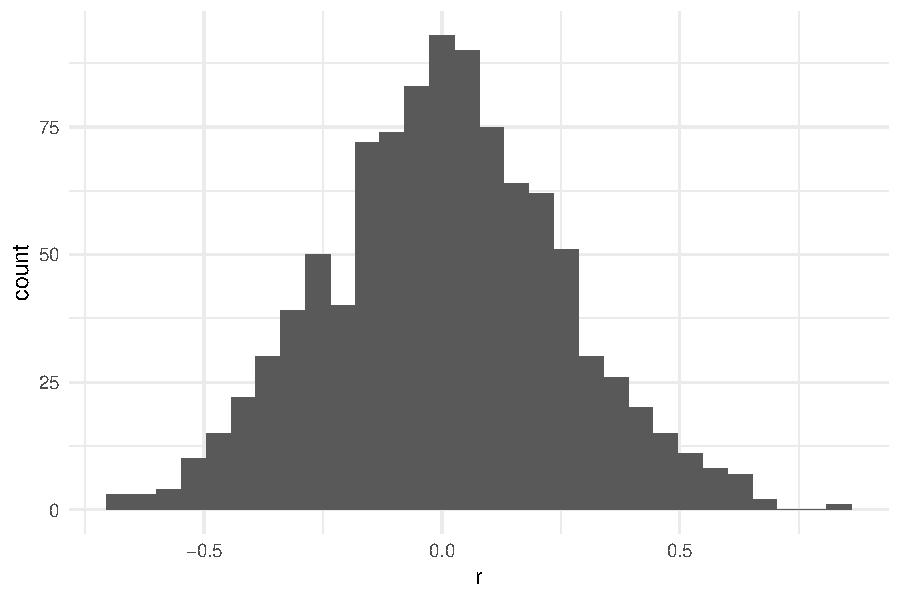
\includegraphics{BB512_files/figure-latex/stochGrowthRate-1} 

}

\caption{1,000 values of $r_m$ drawn from a normal distribution with mean 0.05 and variance 0.1. The dashed line marks $r_m = 0$.}\label{fig:stochGrowthRate}
\end{figure}

When using the equation above to calculate population at time \(t+1\) (\(N_{t+1}\)) from the population at time \(t\) (\(N_t\)), one would draw a random \(r_m\) value from this distribution. Sometimes \(r_m\) will be high, other times it will be low, most of the time it will be from around the middle of the distribution.

Learning outcomes:

\begin{itemize}
\tightlist
\item
  Increased competence in using Excel formulae for mathematical modeling.
\item
  Understanding the concept of stochasticity in simple population models.
\item
  Competence in using mathematical models in Excel to strengthen own understanding of biological processes.
\item
  Understanding how stochasticity relates to (i) uncertainty in the prediction of population trajectories and (ii) probability of (local) extinction.
\end{itemize}

\section{Your task}\label{your-task-4}

Use the Excel worksheet, \href{https://www.dropbox.com/s/1wpixbpgwlh54f0/StochasticPopulationGrowth.xlsx?dl=1}{StochasticPopulationGrowth.xlsx}, to study how stochastic population growth works with this simple model.

In this practical we use the same settings throughout: \(r_m\) is drawn from a normal distribution with \textbf{mean 0.05 and variance 0.1}. Years of growth then only slightly outnumber years of decline (about 56:44). This means a population can grow on average yet still crash by chance, especially when starting size is small.

In the Excel template, first set the mean of \(r_m\) to \textbf{0.05} and the variance to \textbf{0.1} (the template may contain other values), and use a starting population of \textbf{100}.

\begin{enumerate}
\def\labelenumi{\arabic{enumi})}
\tightlist
\item
  Use Excel formulae to calculate deterministic population size through time (25 generations, t = 0 to 25, with starting population of 100), linking to the mean finite population growth rate.
\item
  Use charts to plot the results. (you already did this last time!)
\item
  Use a formula to generate a column of stochastic \(r_m\) values, based on a chosen mean and variance. The formula refers to the cells that hold the mean and the variance of \(r_m\); check where these are in your sheet (in the template they are G10 and G11). In English versions of Excel the function may be written either as \texttt{=NORM.INV(RAND(),\ \$G\$10,\ SQRT(\$G\$11))} (newer versions) or \texttt{=NORMINV(RAND(),\ \$G\$10,\ SQRT(\$G\$11))} (older versions), while in Danish Excel it appears as \texttt{=NORMINV(SLUMP();\ \$G\$10;\ KVROD(\$G\$11))}. If you encounter errors, check whether your copy of Excel expects commas or semi-colons as argument separators and adjust the formula accordingly.
\item
  Use the same procedure as before, to create a stochastic population size vector (stochastic N). Remember to convert \(r_m\) to \(\lambda\) by taking the exponential.
\item
  Compare the two trajectories using a chart.
\item
  Try altering initial population size, mean population growth, and the amount of stochasticity (Variance).
\item
  In this model N is multiplied by \(e^{r_m}\), which is always positive, so N can never reach exactly 0. Instead, we treat the population as (quasi-)extinct if N falls below 1 at any point, i.e.~fewer than one individual is left (the R code below uses the same rule). What happens to extinction risk as stochasticity (variance) increases? What happens when initial N is small? Does the population ALWAYS survive if the mean population growth rate, \(\bar{r_m}\), is \(>\) 0?
\end{enumerate}

Note: Excel re-randomises the random numbers every time you change any cell in the sheet. This is OK, and allows you to explore a stochastic simulation many times.

\section{Simulations in R}\label{simulations-in-r}

Excel is of limited use to really get a feel for this. For the next part we'll use \emph{R}.

If you already have R on your computers you can play along, otherwise take a look at my demonstration in class. I will show how you can use this simulation approach to estimate extinction risk and how this is related to starting population size, mean lambda, and the amount of stochasticity.

You can copy/paste the code below into \emph{R}.

The output of the modelling is shown in Fig. \ref{fig:stochProjection}

Copy-and-paste the code below into a text file (or directly into \emph{R}).

The final line of the code (\texttt{nExtinct/nTrials}) gives you an estimate of extinction probability - the proportion of trials in which the population falls to 1 or fewer individuals at some point, the same rule as in the Excel exercise. The R settings use the same mean (0.05) and variance (0.1) of \(r_m\) as the Excel exercise, but a smaller starting population (10), so that extinctions are common enough to see.

Modify the simulation settings to explore what happens to (i) the plot of population growth and (ii) extinction risk, when you vary \texttt{mean.r} (\(\bar{r_m}\)), the amount of stochasticity (\(\sigma_{r_m}^2\)) (\texttt{var.r}), and the number of generations (\texttt{nGen}).

\begin{Shaded}
\begin{Highlighting}[]
\CommentTok{\#Simulating stochastic geometric population growth rate}

\CommentTok{\#Simulation settings (try changing these)}
\NormalTok{mean.r }\OtherTok{=} \FloatTok{0.05} \CommentTok{\# the mean value of r}
\NormalTok{var.r }\OtherTok{=} \FloatTok{0.1} \CommentTok{\# the variance in r (stochasticity)}
\NormalTok{startPop }\OtherTok{=} \DecValTok{10} \CommentTok{\# pop size at start}
\NormalTok{nGen }\OtherTok{=} \DecValTok{50} \CommentTok{\# number of generations}
\NormalTok{nTrials }\OtherTok{=} \DecValTok{1000} \CommentTok{\# number of repeated simulations}

\DocumentationTok{\#\#\#\#\#\#\#\#\#\#\#\#\#\#\#\#\#\#\#\#\#\#\#\#\#\#\#\#\#\#\#\#\#\#\#\#\#\#\#\#\#\#\#\#\#\#\#\#\#\#\#\#\#\#\#\#\#\#}
\CommentTok{\#If you are unfamiliar with R, don\textquotesingle{}t edit below this line!}
\DocumentationTok{\#\#\#\#\#\#\#\#\#\#\#\#\#\#\#\#\#\#\#\#\#\#\#\#\#\#\#\#\#\#\#\#\#\#\#\#\#\#\#\#\#\#\#\#\#\#\#\#\#\#\#\#\#\#\#\#\#\#}

\NormalTok{pseudoExtinction }\OtherTok{=} \DecValTok{1}

\CommentTok{\# First randomly generate some r values}
\NormalTok{rValues }\OtherTok{\textless{}{-}} \FunctionTok{matrix}\NormalTok{(}\FunctionTok{rnorm}\NormalTok{(nTrials }\SpecialCharTok{*}\NormalTok{ nGen, }
                        \AttributeTok{mean =}\NormalTok{ mean.r, }
                        \AttributeTok{sd =} \FunctionTok{sqrt}\NormalTok{(var.r)),}
                  \AttributeTok{ncol =}\NormalTok{ nTrials,}
                  \AttributeTok{nrow =}\NormalTok{ nGen)}

\CommentTok{\# Use a histogram to see what they look like }
\CommentTok{\# (uncomment the line below)}
\CommentTok{\# hist(rValues,col="grey",main="")}

\CommentTok{\# Now run the simulations to see what the resulting }
\CommentTok{\#population growth looks like}
\NormalTok{trials }\OtherTok{=} \FunctionTok{matrix}\NormalTok{(}\AttributeTok{data =} \ConstantTok{NA}\NormalTok{, }\AttributeTok{nrow =}\NormalTok{ nGen, }\AttributeTok{ncol =}\NormalTok{ nTrials)}
\ControlFlowTok{for}\NormalTok{ (j }\ControlFlowTok{in} \DecValTok{1}\SpecialCharTok{:}\NormalTok{nTrials) \{}
\NormalTok{  popSize }\OtherTok{=}\NormalTok{ startPop}
  \ControlFlowTok{for}\NormalTok{ (i }\ControlFlowTok{in} \DecValTok{2}\SpecialCharTok{:}\NormalTok{nGen) \{}
\NormalTok{    stoch.r }\OtherTok{=}\NormalTok{ rValues[i, j]}
\NormalTok{    popSize }\OtherTok{=} \FunctionTok{append}\NormalTok{(popSize, popSize[i }\SpecialCharTok{{-}} \DecValTok{1}\NormalTok{] }\SpecialCharTok{*} \FunctionTok{exp}\NormalTok{(stoch.r))}
\NormalTok{  \}}
\NormalTok{  trials[, j] }\OtherTok{=}\NormalTok{ popSize}
  \FunctionTok{rm}\NormalTok{(popSize)}
\NormalTok{\}}

\CommentTok{\#Calculate probability of (pseudo)extinction}
\NormalTok{minvals }\OtherTok{\textless{}{-}} \FunctionTok{apply}\NormalTok{(trials, }\DecValTok{2}\NormalTok{, min)}
\NormalTok{nExtinct }\OtherTok{\textless{}{-}} \FunctionTok{length}\NormalTok{(minvals[minvals }\SpecialCharTok{\textless{}=}\NormalTok{ pseudoExtinction])}
\NormalTok{probExtinct }\OtherTok{\textless{}{-}}\NormalTok{ nExtinct }\SpecialCharTok{/}\NormalTok{ nTrials}
\FunctionTok{cat}\NormalTok{(}\StringTok{"Pseudo{-}extinction probability:"}\NormalTok{, }\FunctionTok{round}\NormalTok{(probExtinct, }\DecValTok{3}\NormalTok{), }\StringTok{"}\SpecialCharTok{\textbackslash{}n}\StringTok{"}\NormalTok{)}
\end{Highlighting}
\end{Shaded}

\begin{verbatim}
## Pseudo-extinction probability: 0.058
\end{verbatim}

\subsection{Example stochastic trajectories}\label{example-stochastic-trajectories}

\begin{Shaded}
\begin{Highlighting}[]
\CommentTok{\#Make a plot of the population trajectories}
\FunctionTok{plot}\NormalTok{(}
  \DecValTok{1}\SpecialCharTok{:}\NormalTok{nGen,}
  \FunctionTok{log}\NormalTok{(}\FunctionTok{seq}\NormalTok{(}\FloatTok{0.1}\NormalTok{, }\FunctionTok{max}\NormalTok{(trials), }\AttributeTok{length.out =}\NormalTok{ nGen)),}
  \AttributeTok{type =} \StringTok{"n"}\NormalTok{,}
  \AttributeTok{axes =}\NormalTok{ F,}
  \AttributeTok{xlab =} \StringTok{"Time"}\NormalTok{,}
  \AttributeTok{ylab =} \StringTok{"log(N)"}\NormalTok{,}
  \AttributeTok{ylim =} \FunctionTok{log}\NormalTok{(}\FunctionTok{c}\NormalTok{(}\FloatTok{0.1}\NormalTok{, }\DecValTok{100000}\NormalTok{))}
\NormalTok{)}
\FunctionTok{matlines}\NormalTok{(}\FunctionTok{log}\NormalTok{(trials[, }\DecValTok{1}\SpecialCharTok{:}\FunctionTok{min}\NormalTok{(}\DecValTok{100}\NormalTok{, nTrials)]), }\CommentTok{\# plot up to 100 trajectories}
         \AttributeTok{col =} \StringTok{"\#FF234520"}\NormalTok{,}
         \AttributeTok{lty =} \DecValTok{1}\NormalTok{,}
         \AttributeTok{lwd =} \DecValTok{3}\NormalTok{)}
\FunctionTok{axis}\NormalTok{(}\DecValTok{1}\NormalTok{)}
\FunctionTok{axis}\NormalTok{(}\DecValTok{2}\NormalTok{,}
     \AttributeTok{at =} \FunctionTok{log}\NormalTok{(}\FunctionTok{c}\NormalTok{(}\FloatTok{0.1}\NormalTok{, }\DecValTok{1}\NormalTok{, }\DecValTok{10}\NormalTok{, }\DecValTok{100}\NormalTok{, }\DecValTok{1000}\NormalTok{, }\DecValTok{10000}\NormalTok{, }\DecValTok{100000}\NormalTok{)),}
     \AttributeTok{labels =} \FunctionTok{c}\NormalTok{(}\FloatTok{0.1}\NormalTok{, }\DecValTok{1}\NormalTok{, }\DecValTok{10}\NormalTok{, }\DecValTok{100}\NormalTok{, }\DecValTok{1000}\NormalTok{, }\DecValTok{10000}\NormalTok{, }\DecValTok{100000}\NormalTok{))}
\FunctionTok{abline}\NormalTok{(}\AttributeTok{h =} \FunctionTok{log}\NormalTok{(pseudoExtinction), }\AttributeTok{lty =} \DecValTok{2}\NormalTok{)}
\end{Highlighting}
\end{Shaded}

\begin{figure}

{\centering 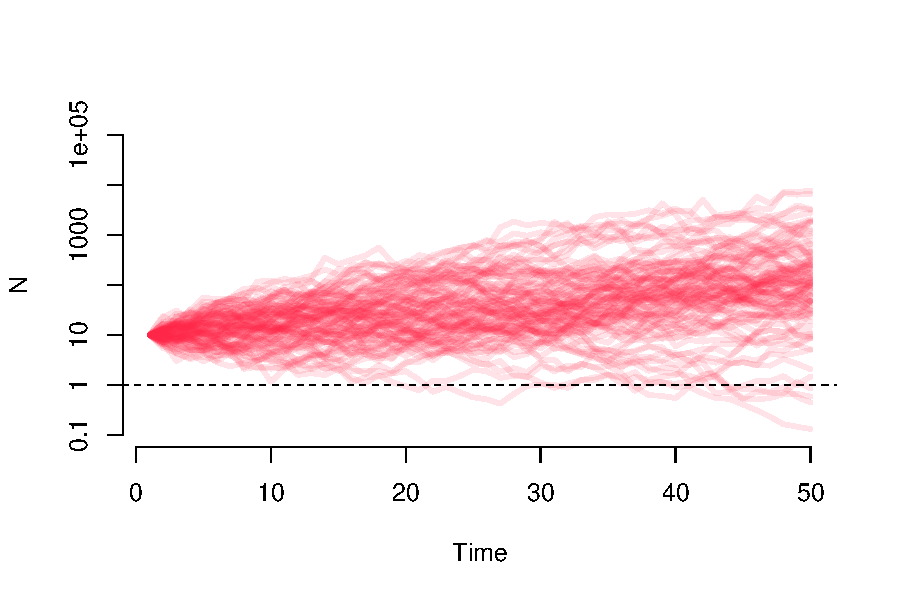
\includegraphics{BB512_files/figure-latex/stochProjection-1} 

}

\caption{An example of stochastic population projection (100 of the 1,000 simulations, 50 generations)}\label{fig:stochProjection}
\end{figure}

\section{Things to try}\label{things-to-try}

Work through these experiments and note what happens to (a) the plot and (b) the extinction probability each time.

\begin{enumerate}
\def\labelenumi{\arabic{enumi}.}
\tightlist
\item
  Run the code as-is. Note the extinction probability and the spread of trajectories.
\item
  Keep \texttt{mean.r\ =\ 0.05} but increase \texttt{var.r} to \textbf{0.5}. How does extinction risk change?
\item
  Reset \texttt{var.r\ =\ 0.1}, then reduce \texttt{startPop} from 10 to \textbf{3}. Does starting population size matter?
\item
  Set \texttt{mean.r\ =\ 0.0} (population neither growing nor shrinking on average). Is extinction certain, unlikely, or somewhere in between?
\item
  \textbf{Challenge:} find a combination of \texttt{mean.r} and \texttt{var.r} where \texttt{mean.r\ \textgreater{}\ 0} but extinction probability exceeds 0.5. What does this tell you?
\end{enumerate}

\section{Questions}\label{questions-4}

\begin{itemize}
\tightlist
\item
  What is the main difference between deterministic and stochastic population growth models?
\item
  Describe how incorporating randomness into the stochastic model makes it more realistic for understanding real-world populations.
\item
  Simulate a scenario where two populations with identical growth rates experience different outcomes due to stochastic factors. Explain the implications of these findings.
\item
  What can this stochastic model tell us about extinction risk and population size?
\item
  What can this stochastic model tell us about extinction risk and environmental variation?
\end{itemize}

\section{Takeaways}\label{takeaways-4}

\begin{itemize}
\tightlist
\item
  Stochasticity introduces variability in trajectories.
\item
  Even when the average growth rate is positive, stochastic variation can create a real risk of extinction.
\item
  Small populations are more vulnerable to random declines and extinction.
\item
  The variance of \(r\) can be as important as its mean for long-term population persistence. This is why conservationists worry about increasing environmental variability, not just declining average conditions.
\item
  Running a model many times (as in the R simulation) reveals the \emph{distribution} of possible outcomes --- a much richer picture than any single trajectory provides.
\end{itemize}

\chapter{Basic logistic population growth}\label{basic-logistic-population-growth}

\section{Background}\label{background-5}

In nature, populations can't grow indefinitely. They eventually reach an upper limit, known as the \emph{carrying capacity} (\(K\)), which represents the maximum number of individuals an environment can support. Factors like available resources, competition, predation, and disease set this limit.

The \textbf{logistic growth model} accounts for this limitation and provides a more realistic picture of population growth. Unlike simpler models, such as exponential growth, that assume unlimited resources, the logistic model reflects how populations slow their growth as they approach the carrying capacity. When the population is small, it can grow quickly, but as it gets closer to the limit, the growth rate slows down. When the population is at carrying capacity the population will not grow (birth rates = death rates).

The model is described by the following equation:

\(N_{t+1} = N_{t} + r_{m} N_{t} \left(1 - \frac{N_{t}}{K}\right)\)

Where:

\begin{itemize}
\tightlist
\item
  \(N_{t+1}\) is the population size at the next time step.
\item
  \(N_t\) is the current population size.
\item
  \(r_m\) is the intrinsic growth rate, or the maximum possible per capita population growth rate.
\item
  \(K\) is the carrying capacity.
\end{itemize}

In this equation, the term \(\left(1 - \frac{N_t}{K}\right)\) slows population growth as the population size \(N_t\) approaches \(K\). If \(N_t = K\), the population stops growing.

This is the discrete-time form of the logistic model used by Neal. Here \(r_m\) is applied once per time step, so when the population is very small (and \(\left(1 - \frac{N_t}{K}\right) \approx 1\)) it grows by a factor of about \(1 + r_m\) each time step. If you remember from earlier exercises that \(\lambda = e^{r_m}\), note that this model treats \(\lambda\) as approximately \(1 + r_m\) instead. For example, with \(r_m = 0.8\), the model gives \(1.8\) where \(e^{0.8} \approx 2.23\). The approximation is good when \(r_m\) is small and poor when it is large. Stepping forward a whole time unit at a time is also what allows the overshoot, oscillations and chaos you will explore below. The continuous-time logistic model always approaches \(K\) smoothly.

As growth rates increase beyond a certain point, the population can exhibit more complex behaviours. At higher growth rates, populations may overshoot the carrying capacity, leading to oscillations as they fluctuate around it. In some cases, the population may show what's called deterministic chaos. This means that while the population fluctuates unpredictably, the system itself is not random --- small changes in initial conditions or growth rates can lead to vastly different outcomes.

This Excel-based exercise will help you explore how changes in the growth rate and carrying capacity affect population dynamics. Though simple, the logistic model provides valuable insights into how populations stabilize, fluctuate, and respond to environmental limits.

Learning outcomes:

\begin{itemize}
\tightlist
\item
  Increased competence in using Excel formulae for mathematical modeling.
\item
  Understanding the parameters of the logistic population growth model.
\item
  Understanding how strikingly different types of population dynamics can result from the same (logistic) model simply by varying the population growth rate parameter.
\item
  Understanding the concept of \emph{deterministic chaos} and how it is different from randomness.
\item
  Competence in using mathematical models in Excel to strengthen own understanding of biological processes.
\end{itemize}

\section{Worked example}\label{worked-example-3}

\subsection{Inputs}\label{inputs-3}

\begin{itemize}
\tightlist
\item
  \texttt{Initial\ N\ =\ 10}
\item
  \texttt{r\_m\ =\ 0.8}
\item
  \texttt{K\ =\ 200}
\end{itemize}

\subsection{Steps}\label{steps-3}

\begin{enumerate}
\def\labelenumi{\arabic{enumi}.}
\tightlist
\item
  Enter these values in the parameter cells.
\item
  Recalculate the model through time.
\item
  Inspect both graphs: population size through time and per-capita growth vs population size.
\end{enumerate}

\subsection{Output and interpretation}\label{output-and-interpretation-3}

The population grows quickly at first, then slows as it approaches \texttt{K}. This produces a sigmoidal curve and a per-capita growth rate that declines linearly with \texttt{N}.

\section{Your Task}\label{your-task-5}

In this exercise, you will explore how changes in key parameters affect population dynamics using the logistic growth model. Follow the steps below to guide your analysis.

\begin{enumerate}
\def\labelenumi{\arabic{enumi}.}
\item
  \textbf{Download the Excel File}\\
  Download and open the Excel file: \href{https://www.dropbox.com/s/oxxyyn4zf4wsvkg/Basic\%20Logistic\%20Growth.xlsx?dl=1}{\texttt{Basic\ Logistic\ Growth.xlsx}}.
\item
  \textbf{Familiarise Yourself with the Spreadsheet}\\
  In the file, you'll see three sections:

  \begin{itemize}
  \tightlist
  \item
    \textbf{Pink Block}: This is where you will input and adjust the model parameters.
  \item
    \textbf{Data Table}: This calculates the population size (\(N\)) and per capita growth rate at each time step. You do not need to edit it.
  \item
    \textbf{Graphs}: These display how the population behaves over time and in relation to the parameters you adjust.
  \end{itemize}
\item
  \textbf{Understand the Parameters}\\
  In the \emph{pink block}, you will find the key parameters of the logistic growth model:

  \begin{itemize}
  \tightlist
  \item
    \texttt{Initial\ N}: The starting population size at time 0 (default = 10).
  \item
    \texttt{r\_m}: The maximum per capita population growth rate (default = 0.8).

    \begin{itemize}
    \tightlist
    \item
      If \(r_m > 0\), the population grows.
    \item
      If \(r_m < 0\), the population shrinks.
    \item
      Biologically, population size cannot fall below zero (but see the footnote in Step 5 --- the spreadsheet does not enforce this).
    \end{itemize}
  \item
    \texttt{K}: The carrying capacity of the population (default = 200).
  \end{itemize}
\item
  \textbf{Explore the Model}\\
  Use the following steps to guide your exploration of population dynamics:
\end{enumerate}

\subsection{Graph 1: Population Size Through Time}\label{graph-1-population-size-through-time}

\begin{itemize}
\item
  \textbf{Step 1}: Examine the default settings in Graph 1, where \texttt{Initial\ N} = 10, \texttt{r\_m} = 0.8, and \texttt{K} = 200.

  \begin{itemize}
  \item
    What is the maximum population size in relation to the carrying capacity?
  \item
    At what time does the population reach its maximum size?
  \end{itemize}
\item
  \textbf{Step 2}: Increase the carrying capacity (\texttt{K}) to 300.\\
  \textbf{Prediction}: What do you expect to happen to the population size over time?

  \textbf{Test}: How does increasing \texttt{K} affect the maximum population size and the time taken to reach it?
\item
  \textbf{Step 3}: Halve the growth rate (\texttt{r\_m}) to 0.4.\\
  \textbf{Prediction}: How will this change affect the population's growth and the time it takes to reach the maximum population size?\\

  \textbf{Test}: What do you observe in the graph?
\item
  \textbf{Step 4}: Increase \texttt{r\_m} to 1.8.

  \begin{itemize}
  \item
    How does the population size change over time?
  \item
    How does the maximum population size compare to the carrying capacity?
  \item
    How would you describe the dynamics of this population (e.g., overshoot, oscillations)?
  \end{itemize}
\item
  \textbf{Step 5}: Experiment with higher values for \texttt{r\_m} (e.g., 2.0, 2.8, 2.9, 3.0).

  \begin{itemize}
  \item
    How do the population dynamics change as \texttt{r\_m} increases?
  \item
    Is there a limit to how high \texttt{r\_m} can be?
  \item
    What happens when \texttt{r\_m} is 2.8 or 3.0\footnote{The behaviour where \texttt{r\_m} values above 3 cause the population to become very negative, is a mathematical artefact caused by numerical instability in the discrete-time logistic growth model. When the growth rate is too high, the population can overshoot its carrying capacity, and the formula's negative feedback term can drive the population to unrealistic, negative values. This issue arises because the model doesn't impose biological constraints, such as preventing population sizes from falling below zero. In real biological systems, such negative values would not occur.}? Are the dynamics predictable or chaotic?
  \end{itemize}
\item
  \textbf{Step 6}: Compare the population trajectory for populations with \texttt{r\_m} = 2.8 and \texttt{r\_m} = 2.81, and then fix \texttt{r\_m} at 2.8 but vary the initial population size by a small amount.

  \begin{itemize}
  \item
    How sensitive are these populations to small changes in \texttt{r\_m} or the initial population size?
  \item
    Would these populations be easy or hard to predict?
  \item
    What kinds of species have high population growth rates like this? How might this relate to managing pest species or diseases?
  \end{itemize}
\end{itemize}

\subsection{Graph 2: Per Capita Growth Rate vs.~Population Size}\label{graph-2-per-capita-growth-rate-vs.-population-size}

\begin{itemize}
\tightlist
\item
  \textbf{Step 1}: Examine Graph 2 with the default settings (\texttt{Initial\ N} = 10, \texttt{r\_m} = 0.8, \texttt{K} = 200).

  \begin{itemize}
  \item
    How does the per capita growth rate change as the population size increases?
  \item
    Where does the per capita growth rate cross the x-axis (population size)?
  \end{itemize}
\item
  \textbf{Step 2}: Modify the carrying capacity (\texttt{K}) to 300 and observe the changes in Graph 2.

  \begin{itemize}
  \item
    How does increasing the carrying capacity affect where the per capita growth rate crosses the x-axis?
  \item
    Does the slope of the per capita growth rate change when you alter \texttt{K}?
  \end{itemize}
\item
  \textbf{Step 3}: Change \texttt{r\_m} to 1.8 and observe how the graph is affected.

  \begin{itemize}
  \item
    How does increasing \texttt{r\_m} affect the shape of the curve?
  \item
    Does the intercept on the x-axis change when you increase \texttt{r\_m}?
  \end{itemize}
\item
  \textbf{Step 4}: Experiment with different values for \texttt{K} and \texttt{r\_m}.

  \begin{itemize}
  \item
    How do changes in \texttt{K} and \texttt{r\_m} together affect the graph?
  \end{itemize}
\end{itemize}

\subsection{Reflection on Graph 2}\label{reflection-on-graph-2}

\begin{itemize}
\tightlist
\item
  \textbf{Step 5}: Compare the per capita growth rate in \textbf{Graph 2} to the population size over time in \textbf{Graph 1}.
  \textbf{Questions}:

  \begin{itemize}
  \item
    How are the two graphs connected?
  \item
    What would the per capita growth rate look like for a population experiencing exponential growth instead of logistic growth?
  \end{itemize}
\end{itemize}

These steps help you visualise how population size and per capita growth rate are interrelated, reinforcing the concepts behind logistic population growth.

These two graphs are different ways to visualize the same model.

It is important that you can make the connections between these graphs.

How would the same plots look for regular exponential growth?

Some useful keywords:

\begin{itemize}
\tightlist
\item
  Oscillation
\item
  Damped oscillation
\item
  Cycle/cyclic dynamics
\item
  Stable-limit cycle (2-point, 3-point limit cycle)
\item
  Chaos/Chaotic dynamics
\item
  Unpredictable/predictable
\end{itemize}

\section{Takeaways}\label{takeaways-5}

\begin{itemize}
\tightlist
\item
  Logistic growth captures density dependence through the carrying capacity \(K\).
\item
  High growth rates can cause overshoot, oscillations, or chaos in discrete-time models.
\item
  Per-capita growth declines linearly with population size in the logistic model.
\end{itemize}

\section{Questions}\label{questions-5}

\begin{itemize}
\item
  In the logistic growth model, what happens to the population growth rate as the population size approaches the carrying capacity (\(K\))? How does this lead to population stability?
\item
  In the logistic growth model, what factors can cause a population to overshoot its carrying capacity temporarily? How does the population respond to such overshooting?
\item
  How can a ballpark knowledge of maximum per capita population growth rate (\(r_m\)) be useful to a population manager?
\item
  What are the key assumptions of the logistic growth model, and how might these assumptions limit its real-world application?
\end{itemize}

\section{Optional: Do this in R.}\label{optional-do-this-in-r.}

You can implement this model in R as follows.
In this code, I have added a line which ensures that population size cannot be negative.

\begin{Shaded}
\begin{Highlighting}[]
\CommentTok{\# Parameters}
\NormalTok{r\_m }\OtherTok{\textless{}{-}} \FloatTok{2.9}  \CommentTok{\# intrinsic growth rate}
\NormalTok{K }\OtherTok{\textless{}{-}} \DecValTok{1000}   \CommentTok{\# carrying capacity}
\NormalTok{N0 }\OtherTok{\textless{}{-}} \DecValTok{10}    \CommentTok{\# initial population size}
\NormalTok{timesteps }\OtherTok{\textless{}{-}} \DecValTok{50}  \CommentTok{\# number of time steps}

\CommentTok{\# Initialize population vector}
\NormalTok{population }\OtherTok{\textless{}{-}} \FunctionTok{numeric}\NormalTok{(timesteps)}
\NormalTok{population[}\DecValTok{1}\NormalTok{] }\OtherTok{\textless{}{-}}\NormalTok{ N0}

\CommentTok{\# Initialize per capita growth rate vector}
\CommentTok{\# Length of one less than population, as it\textquotesingle{}s based on changes}
\NormalTok{per\_capita\_growth }\OtherTok{\textless{}{-}} \FunctionTok{numeric}\NormalTok{(timesteps }\SpecialCharTok{{-}} \DecValTok{1}\NormalTok{)  }

\CommentTok{\# Loop to calculate population at each time step}
\ControlFlowTok{for}\NormalTok{ (t }\ControlFlowTok{in} \DecValTok{2}\SpecialCharTok{:}\NormalTok{timesteps) \{}
  \CommentTok{\# Logistic growth model equation}
\NormalTok{  population[t] }\OtherTok{\textless{}{-}}\NormalTok{ population[t}\DecValTok{{-}1}\NormalTok{] }\SpecialCharTok{+} 
\NormalTok{    (r\_m }\SpecialCharTok{*}\NormalTok{ population[t}\DecValTok{{-}1}\NormalTok{]) }\SpecialCharTok{*}\NormalTok{ (}\DecValTok{1} \SpecialCharTok{{-}}\NormalTok{ (population[t}\DecValTok{{-}1}\NormalTok{] }\SpecialCharTok{/}\NormalTok{ K))}
  
  \CommentTok{\# Ensure population doesn\textquotesingle{}t go negative}
  \ControlFlowTok{if}\NormalTok{ (population[t] }\SpecialCharTok{\textless{}} \DecValTok{0}\NormalTok{) \{}
\NormalTok{    population[t] }\OtherTok{\textless{}{-}} \DecValTok{0}
\NormalTok{  \}}
  
  \CommentTok{\# Calculate per capita growth rate for the previous time step}
  \CommentTok{\# (undefined if the previous population was zero)}
  \ControlFlowTok{if}\NormalTok{ (population[t}\DecValTok{{-}1}\NormalTok{] }\SpecialCharTok{\textgreater{}} \DecValTok{0}\NormalTok{) \{}
\NormalTok{    per\_capita\_growth[t}\DecValTok{{-}1}\NormalTok{] }\OtherTok{\textless{}{-}}\NormalTok{ (population[t] }\SpecialCharTok{{-}}
\NormalTok{                                 population[t}\DecValTok{{-}1}\NormalTok{]) }\SpecialCharTok{/}\NormalTok{ population[t}\DecValTok{{-}1}\NormalTok{]}
\NormalTok{  \} }\ControlFlowTok{else}\NormalTok{ \{}
\NormalTok{    per\_capita\_growth[t}\DecValTok{{-}1}\NormalTok{] }\OtherTok{\textless{}{-}} \ConstantTok{NA}
\NormalTok{  \}}
\NormalTok{\}}

\FunctionTok{par}\NormalTok{(}\AttributeTok{mfrow=}\FunctionTok{c}\NormalTok{(}\DecValTok{1}\NormalTok{,}\DecValTok{2}\NormalTok{))}
\CommentTok{\# Plot 1: Population size through time}
\FunctionTok{plot}\NormalTok{(}\DecValTok{1}\SpecialCharTok{:}\NormalTok{timesteps, population, }\AttributeTok{type =} \StringTok{"o"}\NormalTok{, }\AttributeTok{col =} \StringTok{"blue"}\NormalTok{, }
     \AttributeTok{xlab =} \StringTok{"Time"}\NormalTok{, }\AttributeTok{ylab =} \StringTok{"Population size"}\NormalTok{,}
     \AttributeTok{main =} \StringTok{"Population Size through Time (Logistic Growth Model)"}\NormalTok{)}

\CommentTok{\# Plot 2: Per capita growth rate vs population size}
\FunctionTok{plot}\NormalTok{(population[}\DecValTok{1}\SpecialCharTok{:}\NormalTok{(timesteps}\DecValTok{{-}1}\NormalTok{)], per\_capita\_growth, }
     \AttributeTok{type =} \StringTok{"o"}\NormalTok{, }\AttributeTok{col =} \StringTok{"red"}\NormalTok{, }
     \AttributeTok{xlab =} \StringTok{"Population Size"}\NormalTok{, }
     \AttributeTok{ylab =} \StringTok{"Per Capita Growth Rate"}\NormalTok{,}
     \AttributeTok{main =} \StringTok{"Per Capita Growth Rate vs Population Size"}\NormalTok{)}
\end{Highlighting}
\end{Shaded}

\pandocbounded{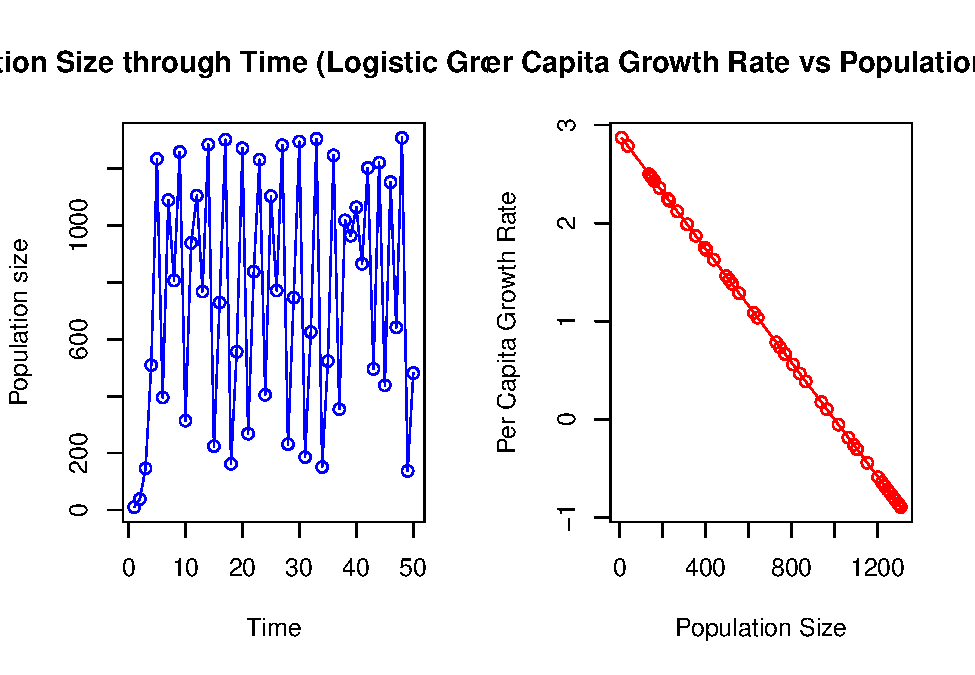
\includegraphics[keepaspectratio]{BB512_files/BB512_files/figure-latex/logistic_optional_r_code-1.pdf}}

\chapter{Deeper into Logistic Growth}\label{deeper-into-logistic-growth}

\section{Background}\label{background-6}

The logistic and exponential growth models are closely related and serve as fundamental tools in understanding population dynamics.

\begin{itemize}
\tightlist
\item
  The \textbf{exponential (geometric)} growth model assumes that populations grow without any environmental constraints, leading to unlimited growth.
\item
  The \textbf{logistic} growth model, on the other hand, incorporates environmental limits, specifically the \textbf{carrying capacity} (\(K\)), which represents the maximum number of individuals the environment can support.
\end{itemize}

\subsection{Linking Logistic and Exponential Growth Models}\label{linking-logistic-and-exponential-growth-models}

The logistic growth model is represented by the following equation (Eqn. 5.2 in Neal):

\(\frac{dN}{dt}=r_m N\left(1-\frac{N}{K}\right)\)

In this model, as the population size \(N\) approaches the carrying capacity \(K\), the term \(\left(1 - \frac{N}{K}\right)\) decreases, slowing the population growth rate until it reaches zero when \(N = K\).

However, if we remove the constraint of a carrying capacity (i.e., set \(K = \infty\)), the model simplifies to the exponential growth equation:

\(\frac{dN}{dt}=r_m N\left(1-\frac{N}{\infty}\right)\)

which simplifies to

\(\frac{dN}{dt}=r_m N\left(1-0\right)\)

which simplifies to

\(\frac{dN}{dt}= r_m N\)

This is the familiar \textbf{geometric (exponential) growth equation} (Eqn. 4.6 in Neal), which assumes unlimited resources and continuous population growth.

The Excel workbook uses Neal's \emph{discrete-time} versions of these models, in which the population is updated once per time step: \(N_{t+1} = N_{t} + r_{m} N_{t}\left(1 - \frac{N_{t}}{K}\right)\) for logistic growth, and \(N_{t+1} = N_{t} + r_{m} N_{t}\) for exponential growth. These use the same \(r_m\) as the continuous equations, but apply it once per whole time step, so \(dN/dt\) is approximated by the change in population size over one time step, \(N_{t+1} - N_{t}\). The same simplification applies: setting \(K = \infty\) turns the discrete logistic model into the discrete exponential model.

The discrete models are approximations of the continuous ones. For a small population, the discrete model multiplies the population by \(1 + r_m\) each time step, whereas the continuous model gives \(\lambda = e^{r_m}\) (e.g.~\(1.8\) vs.~\(2.23\) for \(r_m = 0.8\)). The approximation is good when \(r_m\) is small and poor when it is large. Stepping forward a whole time unit at a time is what makes the overshoot, oscillations, cycles and chaos you will see in Task 1 possible. Because the population cannot ``see'' that it is approaching \(K\) until the next time step, it can overshoot. The continuous logistic model never does this: it always approaches \(K\) smoothly.

\textbf{Take-home Message: The logistic and exponential growth models are closely related. By setting \(K = \infty\), we transition from the logistic model to the exponential model.}

Learning outcomes:

\begin{itemize}
\tightlist
\item
  Increase competence in using Excel for mathematical modeling.
\item
  Understand the relationship between exponential and logistic growth models.
\item
  Learn how models can be adjusted to explore different biological phenomena.
\item
  Develop skills in visualising and interpreting model outputs from different perspectives.
\item
  Strengthen understanding of biological processes by applying mathematical models.
\end{itemize}

\section{Worked example}\label{worked-example-4}

\subsection{Inputs}\label{inputs-4}

\begin{itemize}
\tightlist
\item
  \texttt{r\_m\ =\ 1.2}
\item
  \texttt{K\ =\ 200}
\item
  Worksheet: \texttt{BasicLogistic}
\end{itemize}

\subsection{Steps}\label{steps-4}

\begin{enumerate}
\def\labelenumi{\arabic{enumi}.}
\tightlist
\item
  Set \texttt{r\_m} and \texttt{K} in the parameter block.
\item
  Observe Figure 1 (population through time).
\item
  Observe Figure 2 (per-capita growth vs \texttt{N}).
\item
  Observe Figure 3 (total growth vs \texttt{N}).
\end{enumerate}

\subsection{Output and interpretation}\label{output-and-interpretation-4}

In Figure 1 the population rises quickly and settles at \(K\), overshooting it only very slightly (to about 201) before levelling off. Figures 2 and 3 show the same model from two other perspectives. You will explore what their shapes and axis intercepts tell you in Tasks 2 and 3.

\section{Your Task}\label{your-task-6}

Download the Excel file \href{https://www.dropbox.com/s/4xq399z7skl1akv/Deeper\%20into\%20Logistic\%20Growth.xlsx?dl=1}{\texttt{Deeper\ Into\ Logistic\ Growth.xlsx}}.

Look at the \texttt{BasicLogistic} worksheet and work through the following tasks:

\textbf{Task 1: Population Dynamics (Figure 1)}

\begin{enumerate}
\def\labelenumi{\arabic{enumi}.}
\item
  Experiment with different values of \(r_m\) (e.g., 0.8, 1.2, 1.8, 2.4, 2.7) and observe how the population dynamics change over time in \textbf{Figure 1}.
\item
  Use the following terms to describe the dynamics you see:

  \begin{itemize}
  \tightlist
  \item
    \textbf{Oscillation}, \textbf{damped oscillation}, \textbf{stable cycle}, \textbf{2-point cycle}, \textbf{chaotic}, \textbf{unpredictable}, \textbf{predictable}.
  \end{itemize}
\end{enumerate}

\textbf{Task 2: Per Capita Growth Rate vs.~Population Size (Figure 2)}

\begin{enumerate}
\def\labelenumi{\arabic{enumi}.}
\item
  Examine \textbf{Figure 2}, which shows the per capita growth rate as a function of population size at time \(t\).
\item
  Notice where the line intercepts the x- and y-axes.

  \begin{itemize}
  \tightlist
  \item
    What are these intercepts?
  \item
    How do these intercepts relate to the values of \(r_m\) and \(K\) that you have set?
  \end{itemize}
\item
  Try varying the values for \(r_m\) and \(K\), and note how the graph changes.
\item
  On paper, sketch a graph of the per capita growth rate vs.~population size for a logistic model with \(r_m = 1.5\) and \(K = 250\). Then, verify your sketch by entering these values into the Excel model.
\end{enumerate}

\textbf{Task 3: Population Growth Rate vs.~Population Size (Figure 3)}

\begin{enumerate}
\def\labelenumi{\arabic{enumi}.}
\item
  \textbf{Figure 3} shows the overall population growth rate (\(dN/dt\)) --- the change in population size per unit time. Adjust the values for \(r_m\) and \(K\) and observe how \textbf{Figure 3} changes.
\item
  Answer the following questions:

  \begin{itemize}
  \tightlist
  \item
    At what population sizes is the population growth rate 0 (\(dN/dt = 0\))?
  \item
    At what population size is the growth rate maximized?
  \end{itemize}
\end{enumerate}

\textbf{Task 4: Comparison with Exponential Growth}

\begin{enumerate}
\def\labelenumi{\arabic{enumi}.}
\tightlist
\item
  Now, consider the differences between \textbf{logistic growth} and \textbf{exponential growth}. How would Figures 1, 2, and 3 change when considering exponential growth?
\end{enumerate}

Sketch equivalent graphs for the exponential (geometric) growth model, including:

\begin{itemize}
\tightlist
\item
  \textbf{Fig 1}: Population size (\(N\)) over time (\(t\)).
\item
  \textbf{Fig 2}: Per capita growth rate (\(\frac{1}{N} \frac{dN}{dt}\)) vs.~population size (\(N\)).
\item
  \textbf{Fig 3}: Population growth rate (\(\frac{dN}{dt}\)) vs.~population size (\(N\))
\end{itemize}

\begin{enumerate}
\def\labelenumi{\arabic{enumi}.}
\setcounter{enumi}{1}
\tightlist
\item
  Look at the \textbf{\texttt{Exponential} worksheet} to see how close you were.
\end{enumerate}

\textbf{Task 5: Adding a Time Lag}

\begin{enumerate}
\def\labelenumi{\arabic{enumi}.}
\item
  In the \textbf{\texttt{TimeLag} worksheet}, explore how adding a time lag to the logistic model affects population dynamics. This is the equation we are using: \(\frac{dN}{dt}=r_m N_t\left(1-\frac{N_{t-\tau}}{K}\right)\), where \(\tau\) is the length of the time lag. With \(\tau = 1\), density dependence acts on the population size one time step ago rather than the current population size.
\item
  Adjust the formula in the Excel sheet to incorporate a time lag in the population size (\(N_{t-\tau}\)). The \texttt{dN/dt} column (column C) currently uses the current population size. For a 1-step lag, change the formula in cell C11 to \texttt{=\$B\$5*B11*(1-(B10/\$B\$6))}, so that the density-dependent term uses the population size from the previous time step. Then fill this formula down to the bottom of the column.
\item
  Start with the default \(r_m = 0.6\), which gives smooth convergence to \(K\) in the ordinary logistic model. With the 1-step lag, you should see the population overshoot \(K\) and then show damped oscillations before settling. Now increase \(r_m\) to 1.2. What happens to the oscillations?
\item
  Compare this with the ordinary logistic model (no lag) at the same \(r_m\) values (e.g.~using the \texttt{BasicLogistic} worksheet). This exercise demonstrates how a simple life history trait (such as a time lag) can make a population overshoot and oscillate at growth rates that would otherwise give smooth convergence to \(K\). With a large enough lag or growth rate, the oscillations become sustained cycles.
\end{enumerate}

\section{Questions}\label{questions-6}

\begin{itemize}
\tightlist
\item
  How does increasing or decreasing \(r_m\) affect the shape and behaviour of the population time series in Figure 1? How does it change the per capita growth rate curve in Figure 2 and the population growth rate in Figure 3?
\end{itemize}

\begin{itemize}
\tightlist
\item
  The peak of the parabola in Figure 3 gives the \emph{maximum sustainable yield} (MSY): the largest number of individuals that could be harvested each time step without the population declining. What is the MSY for a population with \(r_m = 0.8\) and \(K = 200\), and at what population size should the population be kept to achieve it? Why might harvesting at exactly the MSY be risky in practice?
\end{itemize}

\begin{itemize}
\tightlist
\item
  In the discrete model, \(N_{t+1} = N_t + dN/dt\). Using what you know about Figure 3, what shape would a plot of \(N_{t+1}\) against \(N_t\) have? Where would it cross the line \(N_{t+1} = N_t\), and why?
\end{itemize}

\begin{itemize}
\tightlist
\item
  What happens to the population dynamics when a time lag is introduced? A time lag could be caused by a long gestation period, or by the need to take a year out before breeding again.
\end{itemize}

\section{Takeaways}\label{takeaways-6}

\begin{itemize}
\tightlist
\item
  Logistic and exponential growth are linked by the carrying capacity term.
\item
  Figures of \(N\) vs.~time, per-capita growth rate vs.~\(N\) and \(dN/dt\) vs.~\(N\) are three views of the same model; you should be able to move between them.
\item
  In discrete time, high \(r_m\) causes overshoot, oscillations, cycles and chaos.
\item
  Time lags can destabilize otherwise stable dynamics.
\end{itemize}

\chapter{Life tables and survivorship types}\label{life-tables-and-survivorship-types}

\section{Background}\label{background-7}

Life tables are powerful analytical tools used in various fields to understand and quantify mortality patterns and life expectancy within populations. Originating in population biology and demography, life tables have found extensive applications in epidemiology, human mortality studies, and even product life-cycle management. By systematically tracking and analysing the survival and mortality rates of individuals within specific cohorts, life tables reveal essential information about population dynamics, age-specific risks, and the factors that influence longevity. When they also record reproduction, they tell us how fast a population grows.

The basic algebra used in life tables is explained in Neal, in the chapters \emph{Life tables and age-specific death rates} and \emph{Age-specific reproduction and population growth rates}, and in the lecture ``Life tables and age-structured population growth''. This practical uses the same notation as Neal and the lecture (see the table below). Gotelli's \emph{A Primer of Ecology} (optional) covers the same material with different symbols: \(g_x\) for \(p_x\), \(b_x\) for \(m_x\) and \(G\) for \(T\).

In addition to providing valuable insights into mortality patterns and life expectancy, life tables also allow us to consider mortality patterns in the context of distinct survivorship types that result from the way mortality risk changes over the life course. Three primary survivorship types are commonly identified, based on survivorship curves (\(l_x\)) plotted on a log scale:

\begin{itemize}
\tightlist
\item
  Type I (convex curve): mortality is low early in life and \textbf{increases} with age. Most individuals survive to old age, and most deaths occur in older age groups. Type I survivorship is seen in humans and other long-lived species with strong parental care and low early-life mortality.
\item
  Type II (straight line): mortality is \textbf{constant} with age, so individuals have about the same chance of dying at any age. Some small mammals and many birds come close to this pattern.
\item
  Type III (concave curve): mortality is high early in life and \textbf{decreases} with age. Survival is low in the early stages of life, but those that survive the vulnerable period are likely to live a long time. Type III survivorship is typical of species that produce many offspring with little parental care, such as many fish and trees.
\end{itemize}

Real species are often mixtures: for example, Dall sheep and many birds have high juvenile mortality (Type III-like), followed by mortality that rises with age in adults (Type I-like).

By identifying and understanding these survivorship types, researchers gain critical insights into the demographic structure of populations and the selective pressures that influence survival and longevity.

Learning outcomes:

\begin{itemize}
\tightlist
\item
  Increased competence in using Excel formulae for mathematical modelling.
\item
  Competence in using mathematical models in Excel to strengthen your own understanding of biological processes.
\item
  Building a cohort life table, and interpreting survivorship (\(l_x\)), survival probability (\(p_x\)), probability of death (\(q_x\)) and life expectancy (\(e_x\)).
\item
  Calculating the net reproductive rate (\(R_0\)), generation time (\(T\)) and the approximate population growth rate (\(r \approx \ln(R_0)/T\)).
\item
  Understanding the three types of survivorship curve and how they relate to the way mortality changes with age.
\item
  Understanding why changes in reproduction early in life matter more than changes late in life (the declining ``force of selection'').
\end{itemize}

\section{Notation}\label{notation}

{\def\LTcaptype{none} % do not increment counter
\begin{longtable}[]{@{}
  >{\raggedright\arraybackslash}p{(\linewidth - 4\tabcolsep) * \real{0.2667}}
  >{\raggedright\arraybackslash}p{(\linewidth - 4\tabcolsep) * \real{0.3000}}
  >{\raggedright\arraybackslash}p{(\linewidth - 4\tabcolsep) * \real{0.4333}}@{}}
\toprule\noalign{}
\begin{minipage}[b]{\linewidth}\raggedright
Symbol
\end{minipage} & \begin{minipage}[b]{\linewidth}\raggedright
Meaning
\end{minipage} & \begin{minipage}[b]{\linewidth}\raggedright
Calculation
\end{minipage} \\
\midrule\noalign{}
\endhead
\bottomrule\noalign{}
\endlastfoot
\(x\) & Age at the start of the interval (\(x = 0\) means age 0 to 1) & \\
\(S_x\) & Number alive at the start of age \(x\) & counted \\
\(l_x\) & Survivorship: probability of surviving from birth to age \(x\) & \(S_x/S_0\) \\
\(p_x\) & Survival probability: probability of surviving from age \(x\) to \(x+1\) & \(S_{x+1}/S_x\), or \(l_{x+1}/l_x\) \\
\(q_x\) & Probability of dying between age \(x\) and \(x+1\) & \(1 - p_x\) \\
\(e_x\) & Life expectancy: further years expected at age \(x\) & \(\left(\sum_{y \ge x} l_y\right)/l_x - 0.5\) \\
\(m_x\) & Female offspring per female aged \(x\) & \\
\(R_0\) & Net reproductive rate: female offspring per female per lifetime (per generation) & \(\sum l_x m_x\) \\
\(T\) & Generation time: mean age of mothers when their daughters are born & \(\sum x l_x m_x / R_0\) \\
\(r\) & Population growth rate per year (approximation) & \(\ln(R_0)/T\) \\
\end{longtable}
}

\section{Worked example}\label{worked-example-5}

The \emph{Worked example} sheet in the spreadsheet is the life table from the lecture: a cohort of 500 newborn females, with \(S_x\) = 500, 400, 200, 50 and 0 at ages 0 to 4, and \(m_x\) = 0, 2, 3, 1 and 0. Click on the cells to see the formulas. For example:

\begin{itemize}
\tightlist
\item
  Survivorship: \(l_1 = 400/500 = 0.8\)
\item
  Survival probability from age 1 to 2: \(p_1 = 200/400 = 0.5\), so \(q_1 = 1 - 0.5 = 0.5\)
\item
  Life expectancy at birth: \(e_0 = (1 + 0.8 + 0.4 + 0.1)/1 - 0.5 = 1.8\) years
\item
  Net reproductive rate: \(R_0 = 0 + 1.6 + 1.2 + 0.1 = 2.9\)
\item
  Generation time: \(T = (1 \times 1.6 + 2 \times 1.2 + 3 \times 0.1)/2.9 = 4.3/2.9 = 1.48\) years
\item
  Growth rate: \(r \approx \ln(2.9)/1.48 = 0.72\) per year, so \(\lambda = e^r \approx 2.05\)
\end{itemize}

Note that \(r = \ln(R_0)/T\) is an approximation. The exact value for this life table (\(r = 0.776\), \(\lambda = 2.17\)) comes from the Euler--Lotka equation or from a matrix model (next practical).

\section{Your task}\label{your-task-7}

Download and open the Excel file \href{https://www.dropbox.com/scl/fi/rriwgom15g2i6mtvm7p77/Life_Tables_Exercises.xlsx?rlkey=09zk9ilepb1sa4bngi8dmdrwc&dl=1}{\texttt{Life\_Tables\_Exercises.xlsx}}.

The file has three worksheets: ``\emph{Life table}'', ``\emph{Survivorship Curves}'' and ``\emph{Worked example}''.

\subsection{Life table}\label{life-table}

Let's start with ``\textbf{Life table}''.

The aim now is to use Excel as a modelling tool to produce a life table.

I have provided some initial data collected from a cohort of animals. I know how many individuals start each year (i.e.~how many ``\textbf{enter} an interval'') and therefore I can see how many survive each year (i.e.~how many ``enter the \textbf{next} interval''). I also know how many female offspring (on average) are produced by each female of each age (\(m_x\)).

Start by calculating survivorship (\(l_x\)). Survivorship is the \textbf{probability of surviving from birth to a particular age}. Therefore, at age 0, \(l_0 = 1\), since everyone is alive at this point. The next value (\(l_1\)) must be calculated based on the number alive at that point. In this case it is \(352/500 = 0.704\). You must generalise this calculation into a formula that can be dragged to fill column \texttt{D} in the worksheet. In algebraic form, the equation is \(l_x = S_x/S_0\).

\textbf{Tip} You need to understand the use of the \texttt{\$} symbol in Excel, and how to drag the selected area to place the formula in the column.

Next, you can calculate the age-specific \textbf{survival probability}, \(p_x\). Note that this is different from \(l_x\). Survival probability is simply the probability that an individual will survive its current age class, i.e.~the probability that an individual currently aged 2 will survive to become age 3. In this case, it is \(254/298 = 0.852\). The calculation is \(p_x = l_{x+1}/l_x\), or \(S_{x+1}/S_x\).

From there you can calculate the age-specific \textbf{probability of death}, \(q_x\). This is simply \(1 - p_x\): the probabilities of survival and death \textbf{must} sum to 1.

Then calculate \textbf{life expectancy}, \(e_x\), in column \texttt{I}: add up the \(l_x\) values from age \(x\) to the end of the table, divide by \(l_x\), and subtract 0.5 (because, on average, individuals that die during a year die halfway through it). For example, in the worked example \(e_1 = (0.8 + 0.4 + 0.1)/0.8 - 0.5 = 1.125\) years. \textbf{Tip} \texttt{=SUM(D3:\$D\$13)/D3-0.5} in cell \texttt{I3} can be dragged down the column.

Now complete the remaining columns, \(l_x m_x\) and \(l_x m_x x\), and use them to calculate (a) the net reproductive rate, \(R_0 = \sum l_x m_x\); (b) the \textbf{generation time}, \(T = \sum x l_x m_x / R_0\); and (c) the approximate population growth rate, \(r \approx \ln(R_0)/T\). Is this population growing, stationary or shrinking?

Refer to the sheet ``\emph{Worked example}'' if you get stuck (click on the cells to see the formulae used there).

\subsubsection{Declining force of selection}\label{declining-force-of-selection}

The force of selection describes the relative importance of events that happen during the life course for fitness (measured, for example, by \(R_0\) or \(r\)).

To investigate this you can do a computer ``experiment'' by altering reproduction at different ages. You can think of these as ``what if?'' experiments, e.g.~``What if there was a mutation that added 1 to reproduction at age 1, or at age 2, etc.?''

Before you start, \textbf{predict}: will adding one daughter at age 2 or at age 8 have the bigger effect on \(R_0\)? Why?

Add 1 to \(m_x\) at one age at a time (put it back before moving to the next age), and record the new value of \(R_0\). Graph your results as age vs.~change in \(R_0\).

What you should see is that changes early in life matter more than changes later in life. (Adding one daughter at age \(x\) raises \(R_0\) by exactly \(l_x\): a female must survive to age \(x\) to have that extra daughter.)

Use \(R_0\), not the approximate \(r\), for this experiment. The approximation \(r = \ln(R_0)/T\) can even fall when reproduction is added late in life, because \(T\) increases; the exact \(r\) always increases, but by less and less with age.

\subsection{Survivorship curves}\label{survivorship-curves}

In the second part of this class we focus on the \textbf{Survivorship Curves} worksheet.

The aim here is to explore how different types of organisms with different ways of life (``\textbf{life history strategies}'') can have qualitatively different kinds of life tables. The most important thing to observe is the difference in \textbf{survivorship curves} (\(l_x\)). These differences become very obvious when you plot the log-transformed survivorship against age.

In the Excel worksheet, I have placed tables showing the fate of cohorts of three populations of different species. Your job now is to calculate the survivorship curve (\(l_x\)) for these species, and take the natural log (using the formula \texttt{=LN(C3)} for the first population, \texttt{=LN(J3)} for the second population, etc.).

You should see that the graphs automatically fill up with lines. These show Type I, II and III survivorship.

Next, calculate the age-specific probability of death (\(q_x\)) and of survival (\(p_x\)). These are the proportions of individuals that \textbf{enter} the age interval that \textbf{do not} and \textbf{do} survive to the end of the interval, respectively. You can calculate them as \texttt{=1-(B4/B3)} and \texttt{=B4/B3} for the first row of the first population.

Plot graphs of these.

Make sure that you are (1) able to ``diagnose'' survivorship type from looking at a graph of \(\ln(l_x)\) vs \(x\); and (2) able to sketch a cartoon of the mortality trajectory if shown one of these survivorship curves.

\section{Questions}\label{questions-7}

\begin{enumerate}
\def\labelenumi{\arabic{enumi}.}
\tightlist
\item
  What are the three main types of survivorship curves, and which organisms typically exhibit each type?
\end{enumerate}

\begin{enumerate}
\def\labelenumi{\arabic{enumi}.}
\setcounter{enumi}{1}
\tightlist
\item
  What does a net reproductive rate (\(R_0\)) of less than 1 signify for a population?
\end{enumerate}

\begin{enumerate}
\def\labelenumi{\arabic{enumi}.}
\setcounter{enumi}{2}
\tightlist
\item
  How does the shape of a survivorship curve reflect trade-offs in life history strategies, typically?
\end{enumerate}

\begin{enumerate}
\def\labelenumi{\arabic{enumi}.}
\setcounter{enumi}{3}
\tightlist
\item
  How is survivorship (\(l_x\)) different from survival probability (\(p_x\))?
\end{enumerate}

\begin{enumerate}
\def\labelenumi{\arabic{enumi}.}
\setcounter{enumi}{4}
\tightlist
\item
  How does altering reproduction or survival/mortality at different ages affect \(R_0\) and population growth rate?
\end{enumerate}

\begin{enumerate}
\def\labelenumi{\arabic{enumi}.}
\setcounter{enumi}{5}
\tightlist
\item
  Two populations have the same \(R_0\), but one has a shorter generation time. Which grows faster per year, and why?
\end{enumerate}

\begin{enumerate}
\def\labelenumi{\arabic{enumi}.}
\setcounter{enumi}{6}
\tightlist
\item
  The probability of dying in a year, \(q_x\), can never be greater than 1, but the force of mortality, \(\mu_x\), can. Why?
\end{enumerate}

\section{Takeaways}\label{takeaways-7}

\begin{itemize}
\tightlist
\item
  Life tables summarise age-specific survival and reproduction in a compact, comparable way.
\item
  Survivorship type reflects how mortality changes with age, and so different life history strategies.
\item
  \(R_0\) is growth per generation; dividing \(\ln(R_0)\) by the generation time \(T\) gives (approximately) the growth rate per year, \(r\).
\item
  Early-life changes usually have the greatest impact on \(R_0\) and population growth.
\end{itemize}

\chapter{Matrix population modelling}\label{matrix-population-modelling}

\section{Background}\label{background-8}

Matrix population models are powerful and widely used tools in population ecology for studying the dynamics of structured populations. Unlike simple growth models that assume every individual is the same, they take into account variation in vital rates (survival, growth and reproduction) across different life stages or age classes. They are particularly well suited to species with distinct life stages, such as plants with seedlings, juveniles and adults, or animals with different age classes.

A matrix population model uses a transition matrix to describe how individuals move between stages, and how many new individuals each stage contributes, over a fixed time step. By incorporating demographic data and life-history traits, these models give a more realistic picture of population dynamics. They are widely used to \emph{project} the future trajectory of a population under stated assumptions, and to assess how vulnerable it is to environmental change and management actions. In this practical, we will assume that one matrix projection corresponds to one year. Each matrix element therefore represents survival, growth, or reproduction over a one-year interval.

This practical aims to give you a good understanding of the basics of their construction and use.

Learning outcomes:

\begin{itemize}
\tightlist
\item
  Competence in constructing life cycle diagrams to represent the life history of real (or theoretical) organisms.
\item
  Understanding how to parameterise life-cycle diagrams and use them to produce a matrix population model.
\item
  Competence in using R to calculate a population growth rate and project a population.
\item
  Understanding how to connect these results to a management question.
\item
  Understanding the logic of ``\emph{in silico} experiments'' to investigate a biological question (mathematical modelling).
\end{itemize}

\section{Your task}\label{your-task-8}

\begin{enumerate}
\def\labelenumi{\arabic{enumi})}
\item
  First, think of an organism you would like to model the dynamics of. It could be a mammal, a bird, a fish, insect or tree \ldots{} real or fantasy.
\item
  Think about their life cycle, and draw it as a life cycle diagram with circles indicating the stages and arrows representing transitions between stages (e.g.~growth) and reproduction. Keep it simple: aim for \textbf{2-3 stages} and no more than about \textbf{7 arrows}. Your diagram must include at least one reproduction arrow and at least one survival arrow. If your model is stage-based, consider whether individuals can stay in the same stage from one year to the next (an arrow that loops back to the same circle).
\end{enumerate}

Things to think about:

\begin{itemize}
\tightlist
\item
  Is it age based or stage based?
\item
  How many stages are there? Can you simplify (e.g.~instead of age in years, you could use life stage)
\item
  If using stages, how are stages defined? E.g. by size, by development, etc.
\item
  Are the survival and fecundity higher in earlier or later life?
\item
  Does the organism ever skip stages?
\item
  Can the organism move ``backwards'' through the life cycle?
\end{itemize}

\begin{enumerate}
\def\labelenumi{\arabic{enumi})}
\setcounter{enumi}{2}
\tightlist
\item
  Next to the arrows, write values for survival probability and fecundity using your biological knowledge. It is fine to use ``ballpark'' estimates. Read the box below before you choose your fecundity values: a reproduction arrow is not simply the number of babies.
\end{enumerate}

\textbf{What goes on a reproduction arrow?}

A matrix entry tells you how many individuals will be in a stage at the \emph{next} census (next year's count) for each individual in a stage \emph{now}. So a reproduction arrow is the number of newborns that will be counted next year per individual this year. That includes whatever survival is needed for those newborns to be counted:

\begin{itemize}
\tightlist
\item
  If you count the population just \textbf{after} breeding (a post-breeding census), the parent must survive the year to breed again before the next count. The entry is the parent's survival × the number of offspring it then produces. For example, an individual that survives the year with probability 0.8 and then has 2 offspring contributes 0.8 × 2 = 1.6 newborns to next year's count.
\item
  If you count just \textbf{before} breeding (a pre-breeding census), the newborns must survive from birth until the next count. The entry is the number of offspring × their first-year survival.
\end{itemize}

Putting the raw number of babies straight into the matrix is the most common mistake in building matrix models (see the lecture, and the chapter ``Pre- and Post-reproduction census'' for a worked comparison). Demographers call this matrix entry \emph{fertility} (Neal: the fertility coefficient); here we use the everyday word fecundity for the same thing.

The model also follows females only (counting daughters), and assumes there is no shortage of mates.

\textbf{Sanity check your numbers}

\begin{itemize}
\tightlist
\item
  Survival and stage-transition probabilities must be between 0 and 1.
\item
  Fecundity (new individuals counted at the next census, per individual per year) can be greater than 1.
\item
  For individuals starting in a given stage, the survival and transition probabilities leaving that stage cannot add up to more than 1. For example, 0.8 staying in the same stage plus 0.7 moving to the next stage is impossible, because it adds up to 1.5. (Fecundity does not count towards this total, because newborns are \emph{added} to the population rather than being a fate of the parent.)
\end{itemize}

Here's an example for a fictional organism.

\begin{figure}
\centering
\pandocbounded{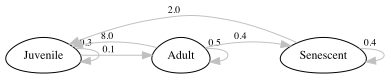
\includegraphics[keepaspectratio,alt={Life cycle diagram of the example organism. Arrows show survival, growth and reproduction transitions.}]{BB512_files/tempLifeCycleDiagram.png}}
\caption{Life cycle diagram of the example organism. Arrows show survival, growth and reproduction transitions.}
\end{figure}

\begin{enumerate}
\def\labelenumi{\arabic{enumi})}
\setcounter{enumi}{3}
\tightlist
\item
  Now you can turn this diagram into a matrix population model by filling in a square of survival/fecundity values.
\end{enumerate}

The life cycle shown above looks like this (below). The matrix describes transitions from time \(t\) to time \(t + 1\), where one time step corresponds to one year.

Interpretation note: \textbf{columns are stages at time \(t\) (from)} and \textbf{rows are stages at time \(t+1\) (to)}.

To place each arrow in the matrix, ask two questions:

\begin{itemize}
\tightlist
\item
  \textbf{FROM which stage does the arrow start?} This gives the \textbf{column}.
\item
  \textbf{TO which stage does the arrow point?} This gives the \textbf{row}.
\end{itemize}

Before you touch R, fill in the blank table below on paper (or in your notes) for your own organism. Name your stages along the top and down the side, then write each arrow's value in the correct cell. Leave a cell as 0 if there is no arrow.

{\def\LTcaptype{none} % do not increment counter
\begin{longtable}[]{@{}lccc@{}}
\toprule\noalign{}
TO ↓ / FROM → & Stage 1 & Stage 2 & Stage 3 \\
\midrule\noalign{}
\endhead
\bottomrule\noalign{}
\endlastfoot
\textbf{Stage 1} & & & \\
\textbf{Stage 2} & & & \\
\textbf{Stage 3} & & & \\
\end{longtable}
}

\textbf{Check your work: every arrow is one non-zero matrix element.}

Count the arrows in your life cycle diagram, then count the non-zero cells in your table. The two numbers must match. If they don't, you have either missed an arrow or put a value in the wrong cell. Also check the column totals against the sanity check above.

For the example organism, the diagram has 7 arrows (including the loops), and the matrix below has 7 non-zero cells.

\[
A = \begin{bmatrix}0.3&8&2 \\0.1&0.5&0 \\0&0.4&0.4 \\\end{bmatrix}
\]

\section{Using R for matrix modelling}\label{using-r-for-matrix-modelling}

Working with matrices is very tedious in Excel. However, in R you can use this information to predict the future dynamics of the population, and estimate population growth rate, and generation time etc.

Open up \textbf{RStudio}, and let's see if we can predict future dynamics. First you will need to install a package called \texttt{popdemo}.

\subsection{Package setup}\label{package-setup}

If you are running this chapter in a fresh R session, you might need to install and/or load the \texttt{popdemo} package.

\begin{Shaded}
\begin{Highlighting}[]
\FunctionTok{install.packages}\NormalTok{(}\StringTok{"popdemo"}\NormalTok{)}
\end{Highlighting}
\end{Shaded}

You only need to install packages once. After that you can load the package for use by using the \texttt{library} function.

\begin{Shaded}
\begin{Highlighting}[]
\FunctionTok{library}\NormalTok{(popdemo)}
\end{Highlighting}
\end{Shaded}

You can put your matrix into R like in the example below (change the numbers to match YOUR model). If your model has fewer, or more, stages then you will need to modify the code a bit. Ask for help if you get stuck.

\begin{Shaded}
\begin{Highlighting}[]
\NormalTok{A }\OtherTok{\textless{}{-}} \FunctionTok{matrix}\NormalTok{(}\FunctionTok{c}\NormalTok{(}
  \FloatTok{0.3}\NormalTok{, }\FloatTok{8.00}\NormalTok{, }\FloatTok{2.00}\NormalTok{,}
  \FloatTok{0.1}\NormalTok{, }\FloatTok{0.50}\NormalTok{, }\FloatTok{0.00}\NormalTok{,}
  \FloatTok{0.0}\NormalTok{, }\FloatTok{0.40}\NormalTok{, }\FloatTok{0.40}
\NormalTok{), }\AttributeTok{ncol =} \DecValTok{3}\NormalTok{, }\AttributeTok{byrow =} \ConstantTok{TRUE}\NormalTok{)}

\NormalTok{stage\_names }\OtherTok{\textless{}{-}} \FunctionTok{c}\NormalTok{(}\StringTok{"Juvenile"}\NormalTok{, }\StringTok{"Adult"}\NormalTok{, }\StringTok{"Senescent"}\NormalTok{)}
\FunctionTok{dimnames}\NormalTok{(A) }\OtherTok{\textless{}{-}} \FunctionTok{list}\NormalTok{(stage\_names, stage\_names)}
\NormalTok{A}
\end{Highlighting}
\end{Shaded}

\begin{verbatim}
##           Juvenile Adult Senescent
## Juvenile       0.3   8.0       2.0
## Adult          0.1   0.5       0.0
## Senescent      0.0   0.4       0.4
\end{verbatim}

\textbf{Important: interpret matrix elements over the chosen time step}

In matrix population models, all transitions occur over a fixed time interval. In this practical, we use a 1-year time step, so:

\begin{itemize}
\tightlist
\item
  survival probabilities are annual
\item
  fecundity is offspring per individual per year
\item
  \(\lambda\) is growth per year
\end{itemize}

\section{Projecting the population}\label{projecting-the-population}

And now you can use the project function to project what happens to the population, then plot it. Look at what happens if you log or don't log the y-axis. First you need to define an initial starting population structure.

In my example, I have 3 stages, so I have 3 values for the initial population sizes.

\subsection{What the projection does}\label{what-the-projection-does}

Let \(\mathbf{n}_t\) be the vector of stage abundances at time \(t\). The population at the next time step is found by multiplying the matrix by that vector:

\[
\mathbf{n}_{t+1} = \mathbf{A}\,\mathbf{n}_t
\]

Each row of \(\mathbf{A}\) answers the question ``where do the individuals in this stage next year come from?'': multiply each entry in the row by the number of individuals in the matching \emph{from} stage (column), then add them up. Using the example matrix and starting population of 10, 5 and 3 individuals in the juvenile, adult and senescent stages:

\[
\begin{bmatrix} n_J \\ n_A \\ n_S \end{bmatrix}_{t=1} =
\begin{bmatrix} 0.3 & 8.0 & 2.0 \\ 0.1 & 0.5 & 0.0 \\ 0.0 & 0.4 & 0.4 \end{bmatrix}
\begin{bmatrix} 10 \\ 5 \\ 3 \end{bmatrix} =
\begin{bmatrix}
(0.3 \times 10) + (8.0 \times 5) + (2.0 \times 3) \\
(0.1 \times 10) + (0.5 \times 5) + (0.0 \times 3) \\
(0.0 \times 10) + (0.4 \times 5) + (0.4 \times 3)
\end{bmatrix} =
\begin{bmatrix} 49 \\ 3.5 \\ 3.2 \end{bmatrix}
\]

So after one year there are 49 juveniles (mostly newborns produced by adults), 3.5 adults and 3.2 senescent individuals. To project two years ahead, we simply repeat the multiplication using the new vector. R does this for us with the \texttt{\%*\%} operator for matrix multiplication:

\begin{Shaded}
\begin{Highlighting}[]
\NormalTok{initial }\OtherTok{\textless{}{-}} \FunctionTok{c}\NormalTok{(}\DecValTok{10}\NormalTok{, }\DecValTok{5}\NormalTok{, }\DecValTok{3}\NormalTok{)}
\NormalTok{A }\SpecialCharTok{\%*\%}\NormalTok{ initial}
\end{Highlighting}
\end{Shaded}

\begin{verbatim}
##           [,1]
## Juvenile  49.0
## Adult      3.5
## Senescent  3.2
\end{verbatim}

The \texttt{popdemo} function \texttt{project} repeats this step as many times as we ask. Here I use it to do a population projection for 10 years (10 time steps). Each step represents one annual cycle of survival, growth, and reproduction.

\textbf{Predict first.} Before you run the projection for your own organism, write down your answers to these questions:

\begin{itemize}
\tightlist
\item
  Do you expect your population to increase, decrease or stay roughly stable? Why?
\item
  Which stage do you expect to become the most abundant?
\end{itemize}

Then run the projection and compare the result with your prediction. If it surprises you, work out why: look at which matrix elements are large and which are small.

\begin{Shaded}
\begin{Highlighting}[]
\NormalTok{pr }\OtherTok{\textless{}{-}}\NormalTok{ popdemo}\SpecialCharTok{::}\FunctionTok{project}\NormalTok{(A, }\AttributeTok{vector =}\NormalTok{ initial, }\AttributeTok{time =} \DecValTok{10}\NormalTok{)}
\end{Highlighting}
\end{Shaded}

Take a look at \texttt{pr}, the projected population. This gives you the total population size, and below that the population sizes in each stage.

\begin{Shaded}
\begin{Highlighting}[]
\NormalTok{pr}
\end{Highlighting}
\end{Shaded}

\begin{verbatim}
## 1 deterministic population projection over 10 time intervals.
## 
##  [1]  18.0000  55.7000  58.4300  85.2570 111.5643 151.4946 203.2634 273.8278
##  [9] 368.4012 495.8572 667.3121
\end{verbatim}

You can access the population sizes of the different stages using \texttt{vec(pr)}.

\begin{Shaded}
\begin{Highlighting}[]
\FunctionTok{vec}\NormalTok{(pr)}
\end{Highlighting}
\end{Shaded}

\begin{verbatim}
##       Juvenile    Adult Senescent
##  [1,]  10.0000  5.00000  3.000000
##  [2,]  49.0000  3.50000  3.200000
##  [3,]  49.1000  6.65000  2.680000
##  [4,]  73.2900  8.23500  3.732000
##  [5,]  95.3310 11.44650  4.786800
##  [6,] 129.7449 15.25635  6.493320
##  [7,] 173.9609 20.60267  8.699868
##  [8,] 234.4093 27.69742 11.721013
##  [9,] 315.3442 37.28964 15.767375
## [10,] 424.4552 50.17924 21.222808
## [11,] 571.2161 67.53514 28.560821
\end{verbatim}

Let's plot this\ldots{}

\begin{Shaded}
\begin{Highlighting}[]
\NormalTok{pop }\OtherTok{\textless{}{-}} \FunctionTok{vec}\NormalTok{(pr)}
\FunctionTok{matplot}\NormalTok{(pop, }\AttributeTok{type =} \StringTok{"l"}\NormalTok{, }\AttributeTok{log =} \StringTok{"y"}\NormalTok{)}
\FunctionTok{legend}\NormalTok{(}\StringTok{"topleft"}\NormalTok{, }\AttributeTok{legend =} \FunctionTok{colnames}\NormalTok{(pop), }
       \AttributeTok{col =} \DecValTok{1}\SpecialCharTok{:}\FunctionTok{ncol}\NormalTok{(pop), }\AttributeTok{lty =} \DecValTok{1}\SpecialCharTok{:}\FunctionTok{ncol}\NormalTok{(pop))}
\end{Highlighting}
\end{Shaded}

\pandocbounded{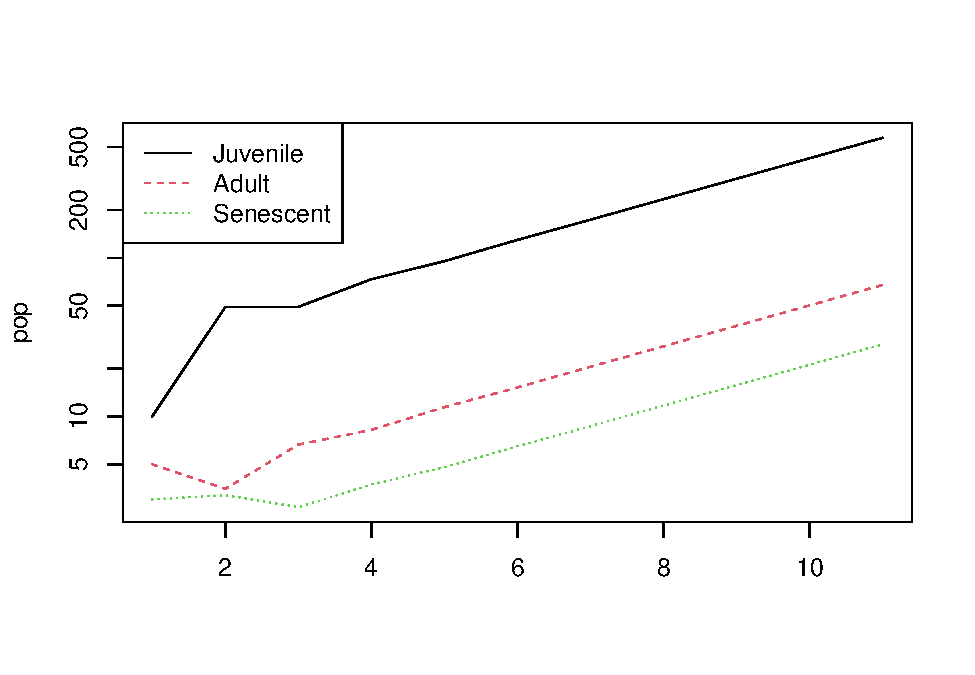
\includegraphics[keepaspectratio]{BB512_files/BB512_files/figure-latex/plotprojectiongraph-1.pdf}}

For the example matrix, the population increases exponentially. Does your own population behave as you predicted? The population growth rate is the so-called ``\emph{dominant eigenvalue}'' of the matrix \textbf{A}.

\subsection{Does the starting population matter?}\label{does-the-starting-population-matter}

Now try the projection again, but with a very different starting population, for example nearly all individuals in the youngest stage, or nearly all in the oldest stage. Keep the matrix the same and change only \texttt{initial}:

\begin{Shaded}
\begin{Highlighting}[]
\NormalTok{initial\_2 }\OtherTok{\textless{}{-}} \FunctionTok{c}\NormalTok{(}\DecValTok{100}\NormalTok{, }\DecValTok{0}\NormalTok{, }\DecValTok{0}\NormalTok{) }\CommentTok{\# change to suit your own life cycle}
\NormalTok{pr\_2 }\OtherTok{\textless{}{-}}\NormalTok{ popdemo}\SpecialCharTok{::}\FunctionTok{project}\NormalTok{(A, }\AttributeTok{vector =}\NormalTok{ initial\_2, }\AttributeTok{time =} \DecValTok{10}\NormalTok{)}
\NormalTok{pop\_2 }\OtherTok{\textless{}{-}} \FunctionTok{vec}\NormalTok{(pr\_2)}
\FunctionTok{matplot}\NormalTok{(pop\_2, }\AttributeTok{type =} \StringTok{"l"}\NormalTok{, }\AttributeTok{log =} \StringTok{"y"}\NormalTok{)}
\end{Highlighting}
\end{Shaded}

\textbf{Predict, then compare.}

\begin{itemize}
\tightlist
\item
  Before you run it: will the \emph{early} part of the trajectory look the same as before? Will the \emph{late} part?
\item
  After you run it: what changes? What eventually becomes the same?
\end{itemize}

Hint: look at the slopes of the lines on the log scale, and at the vertical gaps between them, once the first few years have passed.

\subsection{Growth rate and stable stage distribution}\label{growth-rate-and-stable-stage-distribution}

We can ask R for the \emph{eigenvalues} and \emph{eigenvectors} of the matrix. The dominant eigenvalue is the population growth rate (\(\lambda\)). The corresponding eigenvector gives the stable stage distribution (\emph{SSD}): the expected \emph{proportion} of individuals in each stage class once the population has settled into its long-term pattern. This is exactly what your projections with different starting populations were converging towards.

\textbf{Predict first.} Look at your projection plot. Is \(\lambda\) above 1, below 1, or about 1? Roughly how steep is the line on the log scale? Which stage do you think will have the highest \emph{SSD}?

Because our projection interval is one year, \(\lambda\) represents the annual population growth rate. You can see that in this case, using my example values the population is growing 34.6\% per year.

\begin{Shaded}
\begin{Highlighting}[]
\FunctionTok{eigs}\NormalTok{(A, }\AttributeTok{what =} \FunctionTok{c}\NormalTok{(}\StringTok{"lambda"}\NormalTok{, }\StringTok{"ss"}\NormalTok{))}
\end{Highlighting}
\end{Shaded}

\begin{verbatim}
## $lambda
## [1] 1.345824
## 
## $ss
## [1] 0.85599732 0.10120281 0.04279987
\end{verbatim}

\section{Elasticity}\label{elasticity}

Elasticity analysis asks how responsive the population growth rate (\(\lambda\)) is to a small \emph{proportional} change in each transition of the matrix. A transition with a high elasticity is one where a given percentage change produces a relatively large percentage change in \(\lambda\). The elasticities of all the matrix elements sum to one, so each can be read as that transition's share of the total influence on \(\lambda\). This is useful in management and conservation when we ask questions like, ``which parts of the lifecycle should we focus on to preserve the population?''. The mathematics are beyond this course, and R can calculate the elasticities for us.

\textbf{Predict first.} Looking at your own matrix, which single element do you think \(\lambda\) is most sensitive to? Write it down before running the code.

\begin{Shaded}
\begin{Highlighting}[]
\NormalTok{popdemo}\SpecialCharTok{::}\FunctionTok{elas}\NormalTok{(A)}
\end{Highlighting}
\end{Shaded}

\begin{verbatim}
##             Juvenile      Adult  Senescent
## Juvenile  0.09517264 0.30005511 0.03172421
## Adult     0.33177932 0.19612796 0.00000000
## Senescent 0.00000000 0.03172421 0.01341654
\end{verbatim}

Which transition has the highest elasticity, and what does that tell you about your organism's life cycle? Was your prediction correct? If not, why do you think the biology of your organism led you to the wrong guess? Note that a high elasticity means \(\lambda\) is \emph{sensitive} to that transition, which is not the same as saying it is easy or practical to change in the real world.

\section{In silico experiments: changing the life cycle}\label{in-silico-experiments-changing-the-life-cycle}

Now that we have a model, we can use it as an experimental system. The idea is very simple: you run ``experiments'' on your matrix model (\emph{in silico}, i.e.~on the computer) by asking ``what if'' questions. For example, what would happen if we could increase survival of the juveniles by 20\%? what would happen if adults are hunted more, and thus have a decreased survival by 60\%? what would happen if we provided supplemental food to reproducing females, and increase fecundity by 50\%? etc. Use your imagination!

For each ``what if'' question, follow the same pattern: \textbf{predict} what will happen to \(\lambda\), \textbf{change} the matrix, \textbf{observe} the new \(\lambda\), and \textbf{explain} the difference in biological terms.

In practice, we do that simply by modifying the matrix model. In the following, I am looking at the effect of increasing fecundity in adult and senescent individuals by 50\%:

\begin{Shaded}
\begin{Highlighting}[]
\NormalTok{A\_mod }\OtherTok{\textless{}{-}} \FunctionTok{matrix}\NormalTok{(}\FunctionTok{c}\NormalTok{(}
  \FloatTok{0.3}\NormalTok{, }\FloatTok{8.00}\SpecialCharTok{*}\FloatTok{1.5}\NormalTok{, }\FloatTok{2.00}\SpecialCharTok{*}\FloatTok{1.5}\NormalTok{,}
  \FloatTok{0.1}\NormalTok{, }\FloatTok{0.50}\NormalTok{, }\FloatTok{0.00}\NormalTok{,}
  \FloatTok{0.0}\NormalTok{, }\FloatTok{0.40}\NormalTok{, }\FloatTok{0.40}
\NormalTok{),}
\AttributeTok{byrow =} \ConstantTok{TRUE}\NormalTok{, }\AttributeTok{nrow =} \DecValTok{3}\NormalTok{,}
\AttributeTok{dimnames =} \FunctionTok{list}\NormalTok{(stage\_names, stage\_names)}
\NormalTok{)}

\NormalTok{popdemo}\SpecialCharTok{::}\FunctionTok{eigs}\NormalTok{(A, }\AttributeTok{what =} \StringTok{"lambda"}\NormalTok{)     }\CommentTok{\# original}
\end{Highlighting}
\end{Shaded}

\begin{verbatim}
## [1] 1.345824
\end{verbatim}

\begin{Shaded}
\begin{Highlighting}[]
\NormalTok{popdemo}\SpecialCharTok{::}\FunctionTok{eigs}\NormalTok{(A\_mod, }\AttributeTok{what =} \StringTok{"lambda"}\NormalTok{) }\CommentTok{\# modified}
\end{Highlighting}
\end{Shaded}

\begin{verbatim}
## [1] 1.546586
\end{verbatim}

\begin{Shaded}
\begin{Highlighting}[]
\NormalTok{popdemo}\SpecialCharTok{::}\FunctionTok{elas}\NormalTok{(A\_mod)}
\end{Highlighting}
\end{Shaded}

\begin{verbatim}
##             Juvenile      Adult   Senescent
## Juvenile  0.08514005 0.32540118 0.028380016
## Adult     0.35378119 0.16901684 0.000000000
## Senescent 0.00000000 0.02838002 0.009900705
\end{verbatim}

\section{Your investigation}\label{your-investigation}

Now it is time to work with your own organism. Rather than just running every function once, you will carry out a small investigation of a biological question.

\begin{enumerate}
\def\labelenumi{\arabic{enumi}.}
\tightlist
\item
  \textbf{Project and describe.} Do a projection for your organism, and calculate and interpret \(\lambda\), the stable stage distribution and the elasticities (remember to write down your predictions first).
\item
  \textbf{Choose a question.} Pick a ``what if'' question about your organism. For example:

  \begin{itemize}
  \tightlist
  \item
    What happens if juvenile survival improves?
  \item
    What happens if adults reproduce more?
  \item
    What happens in a bad year (e.g.~lower survival in all stages)?
  \item
    What if reproduction increases at the cost of adult survival?
  \end{itemize}
\item
  \textbf{Predict.} Before changing the model, write down your prediction for what will happen to \(\lambda\), and why.
\item
  \textbf{Change the model.} Modify the appropriate matrix element(s) in a copy of your matrix (e.g.~\texttt{A\_mod}), so that you keep the original for comparison.
\item
  \textbf{Compare.} Calculate \(\lambda\) for both matrices. Was your prediction right?
\item
  \textbf{Explain.} Explain the result in biological terms. Use your elasticity results to help: does the change you made involve a transition with high or low elasticity?
\end{enumerate}

\subsection{An evolutionary experiment}\label{an-evolutionary-experiment}

You can think of lambda (population growth rate) as being a measure of fitness. Imagine that some of your population had a mutation that caused them to have, say, 1 extra baby, but at the expense of reduced survival in one of the younger stages. Would this mutation persist in the population?

First, predict: increasing fecundity is beneficial and decreasing survival is costly. Which effect do you think will win? Then modify the matrix, calculate \(\lambda\) for the mutant life history, and compare it with \(\lambda\) for the original. Does the mutant have a higher or lower \(\lambda\)? What does that suggest about selection on this trade-off? (Comparing \(\lambda\) like this treats it as fitness, which works when growth is density-independent, as it is in this model. With density dependence, as in the logistic growth chapters, things are more complicated.)

\subsection{Questions}\label{questions-8}

\begin{enumerate}
\def\labelenumi{\arabic{enumi}.}
\item
  In the graph showing log-transformed population size through time, what is the significance of the lines being straight after the transient phase?
\item
  Explain how an elasticity analysis of a matrix model can be used to inform the management of a threatened species.
\item
  What are some of the assumptions of a matrix population model? (Hint: some are similar to the assumptions of exponential/geometric growth models. Think about the environment, vital rates, migration and population density.)
\end{enumerate}

\section{Takeaways}\label{takeaways-8}

\begin{itemize}
\tightlist
\item
  Matrix models link life history to population growth through structured vital rates.
\item
  The dominant eigenvalue \(\lambda\) summarizes long-term growth, while its eigenvector gives the stable stage distribution.
\item
  Elasticity analysis and \emph{in silico} experiments turn models into management and evolutionary experiments.
\end{itemize}

\chapter{Pre- and Post-reproduction census}\label{pre--and-post-reproduction-census}

\section{Background}\label{background-9}

Population growth estimates depend on when the census is taken relative to reproduction. A pre-breeding census counts individuals before reproduction; a post-breeding census counts them after reproduction. This changes how survival and fecundity are represented in the projection matrix, even if the underlying biology is the same.

Provided the conversion between the two census types is done correctly, the population growth rate (\(\lambda\)) they produce is identical --- census timing is just a bookkeeping convention, not a biological difference. However, it is easy to get the conversion wrong, and doing so \emph{does} change your estimate of \(\lambda\). This chapter shows both: a correct conversion (same \(\lambda\)), and a common mistake (different \(\lambda\)).

\section{Learning outcomes}\label{learning-outcomes-2}

Learning outcomes:

\begin{itemize}
\tightlist
\item
  Explain the difference between pre-breeding and post-breeding census models.
\item
  Convert a post-breeding matrix to a pre-breeding matrix.
\item
  Recognise that a correct conversion leaves \(\lambda\) unchanged, and explain why.
\item
  Identify how a mis-specified survival or fecundity term changes the resulting \(\lambda\) estimate.
\end{itemize}

\section{Worked example}\label{worked-example-6}

\subsection{Inputs}\label{inputs-5}

We start with a \textbf{post-breeding census} matrix. In a post-breeding census, individuals are counted right after breeding, so the fecundity term for a stage is simply its fecundity scaled by \emph{that stage's own} survival through the year (it has to survive the year in order to be alive, and to breed, at the moment of census).

\begin{Shaded}
\begin{Highlighting}[]
\NormalTok{p0 }\OtherTok{\textless{}{-}} \FloatTok{0.2}
\NormalTok{p1 }\OtherTok{\textless{}{-}} \FloatTok{0.9}
\NormalTok{p2 }\OtherTok{\textless{}{-}} \FloatTok{0.6}
\NormalTok{m2 }\OtherTok{\textless{}{-}} \FloatTok{3.0}
\NormalTok{m3 }\OtherTok{\textless{}{-}} \FloatTok{6.0}

\NormalTok{A1 }\OtherTok{\textless{}{-}} \FunctionTok{matrix}\NormalTok{(}\FunctionTok{c}\NormalTok{(}\FloatTok{0.0}\NormalTok{, m2 }\SpecialCharTok{*}\NormalTok{ p1, m3 }\SpecialCharTok{*}\NormalTok{ p2,}
\NormalTok{               p0, }\FloatTok{0.0}\NormalTok{, }\FloatTok{0.0}\NormalTok{,}
               \FloatTok{0.0}\NormalTok{,p1,}\DecValTok{0}\NormalTok{), }\AttributeTok{byrow =} \ConstantTok{TRUE}\NormalTok{, }\AttributeTok{nrow =} \DecValTok{3}\NormalTok{)}
\end{Highlighting}
\end{Shaded}

\subsection{Steps}\label{steps-5}

\begin{enumerate}
\def\labelenumi{\arabic{enumi}.}
\tightlist
\item
  Define survival and fecundity values.
\item
  Build the projection matrix for one annual time step.
\item
  Use the matrix for projection and comparison tasks below.
\end{enumerate}

\subsection{Output and interpretation}\label{output-and-interpretation-5}

The resulting matrix encodes the post-breeding census assumptions for transitions and fecundity over one year.

Now let's correctly convert this to a \textbf{pre-breeding census} matrix. In a pre-breeding census, individuals are counted just \emph{before} breeding, so two things change:

\begin{itemize}
\tightlist
\item
  Survival transitions shift by one stage, because an individual now has to survive through the year \emph{before} being counted in the next stage at the census.
\item
  Crucially, the fecundity term is no longer scaled by the \emph{parent's} survival (the parent doesn't need to survive to be counted --- the census happens before it would breed again). Instead, it is scaled by \(p_0\), the survival of the \emph{newborn offspring} through to the pre-breeding census.
\end{itemize}

\begin{Shaded}
\begin{Highlighting}[]
\NormalTok{A2 }\OtherTok{\textless{}{-}} \FunctionTok{matrix}\NormalTok{(}\FunctionTok{c}\NormalTok{(}\FloatTok{0.0}\NormalTok{, m2 }\SpecialCharTok{*}\NormalTok{ p0, m3 }\SpecialCharTok{*}\NormalTok{ p0,}
\NormalTok{               p1, }\FloatTok{0.0}\NormalTok{, }\FloatTok{0.0}\NormalTok{,}
               \FloatTok{0.0}\NormalTok{,p2,}\DecValTok{0}\NormalTok{), }\AttributeTok{byrow =} \ConstantTok{TRUE}\NormalTok{, }\AttributeTok{nrow =} \DecValTok{3}\NormalTok{)}
\end{Highlighting}
\end{Shaded}

Compare population growth rates. This uses the \texttt{eigs} function from the \texttt{popdemo} R package.

\begin{Shaded}
\begin{Highlighting}[]
\NormalTok{(popdemo}\SpecialCharTok{::}\FunctionTok{eigs}\NormalTok{(A1, }\AttributeTok{what =} \StringTok{"lambda"}\NormalTok{))}
\end{Highlighting}
\end{Shaded}

\begin{verbatim}
## [1] 1.070261
\end{verbatim}

\begin{Shaded}
\begin{Highlighting}[]
\NormalTok{(popdemo}\SpecialCharTok{::}\FunctionTok{eigs}\NormalTok{(A2, }\AttributeTok{what =} \StringTok{"lambda"}\NormalTok{))}
\end{Highlighting}
\end{Shaded}

\begin{verbatim}
## [1] 1.070261
\end{verbatim}

Notice that \(\lambda\) is (to rounding error) identical for \texttt{A1} and \texttt{A2}. This is not a coincidence: when the conversion between census types is done consistently, it only changes \emph{how} the same underlying survival and reproduction are represented in the matrix --- it does not change the biology, so it cannot change the population's actual growth rate.

\section{A common mistake}\label{a-common-mistake}

It is easy to get the pre-breeding conversion partly right and partly wrong. A very common error is to correctly shift the \emph{survival} transitions to the next stage, but forget to also change the fecundity term --- i.e.~to keep scaling fecundity by the parent's own survival (\(p_1\), \(p_2\)) instead of switching to the offspring survival (\(p_0\)):

\begin{Shaded}
\begin{Highlighting}[]
\NormalTok{A3 }\OtherTok{\textless{}{-}} \FunctionTok{matrix}\NormalTok{(}\FunctionTok{c}\NormalTok{(}\FloatTok{0.0}\NormalTok{, m2 }\SpecialCharTok{*}\NormalTok{ p1, m3 }\SpecialCharTok{*}\NormalTok{ p2,}
\NormalTok{               p1, }\FloatTok{0.0}\NormalTok{, }\FloatTok{0.0}\NormalTok{,}
               \FloatTok{0.0}\NormalTok{,p2,}\DecValTok{0}\NormalTok{), }\AttributeTok{byrow =} \ConstantTok{TRUE}\NormalTok{, }\AttributeTok{nrow =} \DecValTok{3}\NormalTok{)}

\NormalTok{(popdemo}\SpecialCharTok{::}\FunctionTok{eigs}\NormalTok{(A3, }\AttributeTok{what =} \StringTok{"lambda"}\NormalTok{))}
\end{Highlighting}
\end{Shaded}

\begin{verbatim}
## [1] 1.863632
\end{verbatim}

This looks like a small, easy-to-miss slip --- only the fecundity row is ``wrong'', and the matrix still looks like a sensible pre-breeding matrix. But it produces a substantially different (and incorrect) estimate of \(\lambda\), compared to the correctly-converted \texttt{A2}.

\section{Your task}\label{your-task-9}

\begin{itemize}
\tightlist
\item
  Confirm that \texttt{A1} and \texttt{A2} give (to rounding error) the same \(\lambda\). Explain, in your own words, why a \emph{correct} change of census timing should not change the underlying population growth rate.
\item
  Compare \texttt{A2} (correct pre-breeding matrix) and \texttt{A3} (the common mistake). Which specific matrix entries differ, and why does that particular mistake push \(\lambda\) so far from the correct value?
\item
  Modify one survival probability (e.g., \texttt{p1}) and re-build \texttt{A1}, \texttt{A2}, and \texttt{A3}. Does the correct conversion (\texttt{A1} vs \texttt{A2}) still agree? Does the size of the error from the mistake (\texttt{A2} vs \texttt{A3}) grow, shrink, or stay about the same?
\end{itemize}

\section{Takeaways}\label{takeaways-9}

\begin{itemize}
\tightlist
\item
  Census timing (pre- vs.~post-breeding) changes how fecundity and survival are encoded in the matrix, but a \emph{correctly done} conversion between the two gives the same \(\lambda\) --- timing alone is a bookkeeping choice, not a biological difference.
\item
  However, small errors in how survival or fecundity terms are calculated for a given census type are easy to make and can substantially bias your \(\lambda\) estimate.
\item
  The general lesson extends beyond census timing: the specific method used to calculate stage-specific survival and reproduction values for a matrix model matters. Applying the wrong calculation will bias your estimates, even if the matrix ``looks'' reasonable.
\end{itemize}

\chapter{Life Table Response Experiments}\label{life-table-response-experiments}

\section{Introduction}\label{introduction}

A Life Table Response Experiment (LTRE), in matrix population modelling, is a technique used to analyse how differences in demographic parameters between two or more populations or ``treatments'' contribute to differences in their overall growth rate. It's particularly useful for understanding how specific factors like survival rates, fecundity, or other stage-to-stage transitions influence the growth or decline of a population under different conditions.

The method involves comparing matrix models of the populations in question and decomposing the differences in growth rates different models into contributions from individual matrix elements. This approach provides insights into which life cycle stages or transitions are most important for population growth and can inform conservation or management strategies.

\section{Learning outcomes}\label{learning-outcomes-3}

Learning outcomes:

\begin{itemize}
\tightlist
\item
  Explain the purpose of an LTRE and when it is useful.
\item
  Quantify how matrix element changes contribute to \(\lambda\) differences.
\item
  Interpret LTRE output in a biological or management context.
\end{itemize}

\section{Set up}\label{set-up}

For the core LTRE analysis you need \texttt{popbio} (for the \texttt{LTRE} function) and \texttt{popdemo} (for the \texttt{eigs} function used to compare growth rates).
The diagram-export packages are optional and only needed if you want to regenerate the life-cycle diagram image.

\begin{Shaded}
\begin{Highlighting}[]
\CommentTok{\# Core packages (required)}
\FunctionTok{install.packages}\NormalTok{(}\FunctionTok{c}\NormalTok{(}\StringTok{"popbio"}\NormalTok{, }\StringTok{"popdemo"}\NormalTok{))}
\FunctionTok{library}\NormalTok{(popbio)}
\FunctionTok{library}\NormalTok{(popdemo)}

\CommentTok{\# Optional packages (only for rebuilding the diagram figure)}
\FunctionTok{install.packages}\NormalTok{(}\FunctionTok{c}\NormalTok{(}\StringTok{"Rage"}\NormalTok{, }\StringTok{"DiagrammeRsvg"}\NormalTok{, }\StringTok{"rsvg"}\NormalTok{))}
\FunctionTok{library}\NormalTok{(Rage)}
\FunctionTok{library}\NormalTok{(DiagrammeRsvg)}
\FunctionTok{library}\NormalTok{(rsvg)}
\end{Highlighting}
\end{Shaded}

\section{A worked example}\label{a-worked-example}

In this example, we consider a two-stage matrix model to analyse, say, squirrel populations in two different geographic locations. The first, a reference population from Location A, represents an area with favourable environmental conditions. The matrix model for this population distinguishes between juveniles (J) and adults (A), incorporating probabilities for juveniles maturing into adults (0.5) and adults surviving and staying adult (0.6), as well as the fecundity rate (2.3), which is the number of juveniles produced by an adult.

\begin{Shaded}
\begin{Highlighting}[]
\NormalTok{matA }\OtherTok{\textless{}{-}} \FunctionTok{matrix}\NormalTok{(}\FunctionTok{c}\NormalTok{(}\FloatTok{0.1}\NormalTok{,}\FloatTok{2.3}\NormalTok{,}
                 \FloatTok{0.5}\NormalTok{,}\FloatTok{0.6}\NormalTok{), }\AttributeTok{nrow =} \DecValTok{2}\NormalTok{, }\AttributeTok{ncol =} \DecValTok{2}\NormalTok{, }\AttributeTok{byrow =} \ConstantTok{TRUE}\NormalTok{)}

\NormalTok{matA }\OtherTok{\textless{}{-}} \FunctionTok{round}\NormalTok{(matA, }\DecValTok{2}\NormalTok{)}
\end{Highlighting}
\end{Shaded}

\pandocbounded{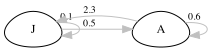
\includegraphics[keepaspectratio]{BB512_files/tempLifeCycleDiagramLTRE.png}}

The treatment population, from Location B, experiences generally worse environmental conditions during the spring which particularly impacts the juvenile stages, and includes an effect on fecundity (e.g.~via neonatal maternal energy allocation). The two matrices can be created in R as follows. Compare the values in the matrix, to the values in the life cycle diagram.

\begin{Shaded}
\begin{Highlighting}[]
\NormalTok{A\_ref }\OtherTok{\textless{}{-}} \FunctionTok{matrix}\NormalTok{(}\FunctionTok{c}\NormalTok{(}\FloatTok{0.1}\NormalTok{,}\FloatTok{2.3}\NormalTok{,}
                  \FloatTok{0.5}\NormalTok{,}\FloatTok{0.6}\NormalTok{), }\AttributeTok{nrow =} \DecValTok{2}\NormalTok{, }\AttributeTok{ncol =} \DecValTok{2}\NormalTok{, }\AttributeTok{byrow =} \ConstantTok{TRUE}\NormalTok{)}

\NormalTok{A\_treat }\OtherTok{\textless{}{-}} \FunctionTok{matrix}\NormalTok{(}\FunctionTok{c}\NormalTok{(}\FloatTok{0.1}\NormalTok{,}\FloatTok{1.3}\NormalTok{,}
                    \FloatTok{0.2}\NormalTok{,}\FloatTok{0.7}\NormalTok{), }\AttributeTok{nrow =} \DecValTok{2}\NormalTok{, }\AttributeTok{ncol =} \DecValTok{2}\NormalTok{, }\AttributeTok{byrow =} \ConstantTok{TRUE}\NormalTok{)}
\end{Highlighting}
\end{Shaded}

\subsection{Comparing matrices}\label{comparing-matrices}

Before we dig into the formal LTRE, it is useful to compare the two matrices, \texttt{A\_ref} and \texttt{A\_treat}, to see how they are different from each other.

We can check what overall difference there is between the matrix in a couple of ways.

Firstly, we can examine the differences in the individual transition rates between the matrices by subtracting one from the other.

\begin{Shaded}
\begin{Highlighting}[]
\NormalTok{A\_ref }\SpecialCharTok{{-}}\NormalTok{ A\_treat}
\end{Highlighting}
\end{Shaded}

\begin{verbatim}
##      [,1] [,2]
## [1,]  0.0  1.0
## [2,]  0.3 -0.1
\end{verbatim}

Next, we can ask what impact these differences have on the population growth rate (lambda).
Note that putting the command in parentheses tells R to both create the new object (e.g.~\texttt{lambdaA1}) \textbf{and} print the result to the screen.

\begin{Shaded}
\begin{Highlighting}[]
\NormalTok{(lambda\_A\_ref }\OtherTok{\textless{}{-}}\NormalTok{ popdemo}\SpecialCharTok{::}\FunctionTok{eigs}\NormalTok{(A\_ref, }\AttributeTok{what =} \StringTok{"lambda"}\NormalTok{))}
\end{Highlighting}
\end{Shaded}

\begin{verbatim}
## [1] 1.451136
\end{verbatim}

\begin{Shaded}
\begin{Highlighting}[]
\NormalTok{(lambda\_A\_treat }\OtherTok{\textless{}{-}}\NormalTok{ popdemo}\SpecialCharTok{::}\FunctionTok{eigs}\NormalTok{(A\_treat, }\AttributeTok{what =} \StringTok{"lambda"}\NormalTok{))}
\end{Highlighting}
\end{Shaded}

\begin{verbatim}
## [1] 0.991608
\end{verbatim}

We could express this as a difference, or as a proportional difference.

The difference in growth rates between the matrices is 0.46.

\begin{Shaded}
\begin{Highlighting}[]
\NormalTok{(lambdaDiff }\OtherTok{\textless{}{-}}\NormalTok{ lambda\_A\_ref }\SpecialCharTok{{-}}\NormalTok{ lambda\_A\_treat)}
\end{Highlighting}
\end{Shaded}

\begin{verbatim}
## [1] 0.4595278
\end{verbatim}

This is a 32\% reduction, compared to the reference matrix.

\begin{Shaded}
\begin{Highlighting}[]
\NormalTok{(lambdaDiff}\SpecialCharTok{/}\NormalTok{lambda\_A\_ref) }\SpecialCharTok{*} \DecValTok{100}
\end{Highlighting}
\end{Shaded}

\begin{verbatim}
## [1] 31.66677
\end{verbatim}

So far, so good. We can see that treatment reduces the population growth rate, but we don't know exactly how. There are 3 changes in the matrix. Which of these changes is most instrumental in driving change in the population growth rate?

\subsection{Contributions from individual matrix elements}\label{contributions-from-individual-matrix-elements}

The objective of the LTRE (Life Table Response Experiment) analysis in this context is to understand the impact of these environmental differences on the difference in population growth rate between the two populations. This is important because identifying the specific life history traits (i.e.~the individual transitions, represented by individual elements of the matrix, such as survival or fecundity) that are most sensitive to environmental changes allows us to pinpoint the key drivers of population dynamics.

By understanding where differences in growth rate originate, we can make more informed decisions about conservation and management strategies. For instance, if the analysis shows that adult survival has a larger impact on growth rate than fecundity, conservation efforts can be more effectively focused on improving adult survival rates rather than fecundity. Conversely, if juvenile survival or fecundity is more influential, efforts might be better directed towards enhancing these aspects. This targeted approach ensures that resources are allocated efficiently, and interventions are tailored to address the most critical factors affecting the population's viability under varying environmental conditions.

By comparing the two models, we can decompose the differences in the overall growth rate (\(\lambda\)) between the baseline (Location A) and the modified model (Location B). This analysis will specifically highlight how changes in adult survival and fecundity in the less favourable environment of Location B contribute to any differences in population growth rates compared to the more favourable conditions in Location A. Such insights are crucial for developing effective management and conservation strategies, particularly in understanding the relative importance of different life stages and demographic parameters under varying environmental conditions.

\begin{Shaded}
\begin{Highlighting}[]
\NormalTok{popbio}\SpecialCharTok{::}\FunctionTok{LTRE}\NormalTok{(A\_treat,A\_ref)}
\end{Highlighting}
\end{Shaded}

\begin{verbatim}
##            [,1]        [,2]
## [1,]  0.0000000 -0.20832964
## [2,] -0.3214229  0.06636876
\end{verbatim}

This summary quantifies the relative importance (and direction) of the effect of the differences between the two matrices on the difference in population growth rate.
One of the changes actually has a positive impact on growth rate, but this is opposed by the other two changes. The most important of these two is the lower left element, which represents the ontogenetic development from juvenile to adult stage.

\section{Relationship with elasticity analysis}\label{relationship-with-elasticity-analysis}

There are similarities between LTRE analysis and elasticity analysis. Comparing LTRE with elasticity analysis reveals some distinct advantages of LTRE in certain contexts.

LTRE can handle comparisons where changes occur in multiple life history parameters simultaneously, providing a more comprehensive view of the potential impacts of various factors on population dynamics. This is in contrast to elasticity analysis, which examines the sensitivity of the population growth rate to small changes in individual demographic rates and assumes other parameters remain constant.

Therefore, LTRE is more directly applicable for evaluating and comparing the impacts of different management strategies or environmental changes that simultaneously affect several demographic traits. It allows for a more nuanced understanding of how specific interventions (like changes in fecundity or survival rates) will influence the population. This is crucial for making informed decisions in conservation and wildlife management.

In summary, while elasticity analysis is valuable for understanding the inherent sensitivity of a population's growth rate to changes in its life cycle processes, LTRE can be a more useful tool for analysing the more complex effects of environmental variations or different management strategies on population dynamics.

\section{Your task}\label{your-task-10}

\begin{itemize}
\tightlist
\item
  Modify one element in \texttt{A\_treat} and predict which LTRE contribution will change most.
\item
  Re-run \texttt{popbio::LTRE} and check whether your prediction matches the output.
\end{itemize}

\section{Takeaways}\label{takeaways-10}

\begin{itemize}
\tightlist
\item
  LTRE decomposes \(\lambda\) differences into contributions from specific transitions.
\item
  It complements elasticity analysis by focusing on actual changes between scenarios.
\end{itemize}

\chapter{How many eggs should a bird lay?}\label{how-many-eggs-should-a-bird-lay}

\section{Background}\label{background-10}

Trade-offs are inherent compromises in biology, where allocating limited resources to one trait may come at the expense of another. Organisms face these trade-offs when making crucial life-history decisions. One classic example is the British ornithologist David Lack's clutch size trade-off, where bird species must balance between producing more eggs with reduced individual investment or fewer eggs with higher individual investment. In other words, although it may be beneficial to have many offspring, the survival of those offspring will decline if they cannot be cared for.

Understanding such trade-offs sheds light on the fascinating strategies that organisms employ to optimize their fitness and evolutionary success.

Learning outcomes:

\begin{itemize}
\tightlist
\item
  Calculate the expected number of surviving offspring from clutch size and chick survival.
\item
  Explain how a trade-off between offspring number and offspring survival produces an intermediate optimum.
\item
  Predict how the optimum changes when the environment, or the cost of breeding to the parents, changes.
\end{itemize}

\section{Before you start: predict}\label{before-you-start-predict}

Before you calculate anything, make a prediction and write it down: will a big bird that lays \textbf{10 eggs} raise more surviving chicks than one that lays \textbf{4 eggs}, or fewer? Why? You will check your prediction below.

\section{Your task}\label{your-task-11}

The big bird (\emph{Bigus canarius}) (Fig \ref{fig:bigbird}) can lay up to 10 eggs per breeding season. If there is only 1 egg, the probability that the parents can adequately feed the chick and ensure it survives is very high (0.9). However, as the number of siblings increases, the amount of energy and food that the parents can dedicate to caring for \emph{each} chick decreases, and the probability of survival therefore declines . With a clutch size of 10 eggs, there is so little food \emph{per chick} that the survival rates are close to zero.

\begin{figure}

{\centering 
\includegraphics[width=0.5\linewidth]{images/bigbird} 

}

\caption{Big bird, *Bigus canarius*}\label{fig:bigbird}
\end{figure}

A recent study gathered data on chick survival probability as a function of number of eggs in the nest. These are given in the table below.

{\def\LTcaptype{none} % do not increment counter
\begin{longtable}[]{@{}ll@{}}
\toprule\noalign{}
Eggs & Survival probability \\
\midrule\noalign{}
\endhead
\bottomrule\noalign{}
\endlastfoot
1 & 0.90 \\
2 & 0.85 \\
3 & 0.82 \\
4 & 0.70 \\
5 & 0.50 \\
6 & 0.30 \\
7 & 0.22 \\
8 & 0.15 \\
9 & 0.10 \\
10 & 0.05 \\
\end{longtable}
}

Use these data to plot a graph in Excel with number of eggs on the x-axis and survival probability on the y-axis.

Now, in another column in Excel, calculate, given the chick survival probability, what the expected number of surviving chicks will be for a big bird laying between 1 and 10 eggs\footnote{This may require some thought!}.

Plot your result on another graph with number of eggs on the x-axis and number of surviving offspring on the y-axis.

What do you notice? What is the optimum number of eggs to lay?

Advanced: What happens to the optimum as you change the relationship between clutch size and survival?

\section{Assumptions}\label{assumptions}

This simple model assumes that every egg hatches, that every chick in a nest has the same chance of surviving, that we count only one breeding season, and that laying and raising more eggs has no cost to the parents' own survival. Question 3 relaxes the last assumption.

\section{Questions}\label{questions-9}

\begin{enumerate}
\def\labelenumi{\arabic{enumi}.}
\tightlist
\item
  What is Lack's hypothesis? Does the big bird's optimum support it?
\item
  In a good food year, each chick's survival probability in clutches of 5 or more eggs is 0.2 higher (for example, 0.50 becomes 0.70). Recalculate. What is the best clutch size now, and why?
\item
  Raising chicks is costly for the parents. Suppose the probability that a parent survives to breed again next year is \(0.8 - 0.08 \times \text{eggs}\) (so 0.72 with 1 egg, and 0.48 with 4 eggs). On average, a parent then breeds \(1 / (1 - \text{parent survival})\) times in its life. Calculate the number of surviving chicks over a parent's whole life for each clutch size. Does the best clutch size change? What does this mean for Lack's hypothesis?
\item
  (Discussion) Birds also trade off the number of eggs against the size of each egg. What would you need to add to this model to study that trade-off?
\end{enumerate}

\section{Takeaways}\label{takeaways-11}

\begin{itemize}
\tightlist
\item
  Trade-offs often produce intermediate optimal strategies.
\item
  Expected reproductive success depends on both offspring number and survival probability.
\item
  If raising young costs the parents' future survival, the best clutch is smaller than the one that produces the most surviving young in a single season.
\end{itemize}

\chapter{Trade-offs and the declining force of selection}\label{trade-offs-and-the-declining-force-of-selection}

\emph{Why does evolution care less and less about you as you age? Because fewer individuals survive to late ages, selection acts more weakly on late life, and trade-offs then let early benefits win over late costs.}

\section{Background}\label{background-11}

An important kind of trade off are those which occur between processes in early and late life. For example, it may be beneficial to increase reproduction at younger ages, but this might lead to increased risk of death at older ages. A mechanism for this could be that limited resources are allocated to producing offspring rather than maintaining/repairing the body.

The balance of the trade off between these early and late life processes is shaped by the \textbf{force of selection}: how much a small change in survival or reproduction at a given age changes fitness. Crucially, the force of selection tends to decline with age meaning that late-life processes are not as important as early-life processes. This means that a mutation giving a modest reproductive advantage at an early age, alongside a harmful or even deadly effect late in life can be ``seen'' by natural selection as advantageous. This idea is called \textbf{antagonistic pleiotropy} (Williams 1957): one gene with a good effect early in life and a bad effect later.

This highlights the significance of early-late life trade-offs and their role in shaping aging patterns in various organisms. Understanding this concept is essential for comprehending life history evolution, aging, and longevity across species.

The aim of this exercise is to gain an understanding of early-life late-life trade offs and to understand why events early in life tend to be much more important to evolution than those that happen later in life.

Learning outcomes:

\begin{itemize}
\tightlist
\item
  Calculate how a change in fertility or survival at a given age changes fitness (\(R_0\)).
\item
  Explain why the force of selection declines with age, and why this lets genes with early benefits and late costs spread.
\item
  Explain why survival after reproduction has ended has little or no effect on fitness in this model.
\end{itemize}

\section{Before you start: predict}\label{before-you-start-predict-1}

Recall that fitness can be measured as \(R_0 = \sum l_x m_x\), where \(l_x\) is the probability of surviving from birth to age \(x\), and \(m_x\) is the number of offspring produced at age \(x\).

Before you open the spreadsheet, make a prediction and write it down: will \textbf{one extra offspring at age 1} or \textbf{one extra offspring at age 20} raise \(R_0\) more? Why? You will check your prediction in the tasks below.

\section{Your task}\label{your-task-12}

Open the Excel file \href{https://www.dropbox.com/scl/fi/972ie76xj7nb9ni61n6ry/Trade_Offs_And_Force_Of_Selection.xlsx?rlkey=jmnpi05n8dicpqt3z8b0hbjhw&dl=0}{TradeOffsAndForceOfSelection.xlsx}.

This file shows a simplified life table, following a cohort of 1000 individuals for a fictional creature.

Survival rates from year to year are set to be 0.8 (i.e.~80\% make it through to the next year). This fixed, constant survival rate leads to an exponentially declining survival curve, illustrated with a chart in the Excel file. Fertility (i.e.~the number of babies produced per year) is set to be 10 per year.

In the spreadsheet, the \textbf{Survival} value in each row is the probability of surviving \emph{into} that age from the age before. So setting Survival to 0 in the age-25 row means that nobody reaches age 25. (The Survival value in the age-1 row is not used: the cohort starts at age 1.)

The product of survivorship (\(l_x\)) and fertility (\(m_x\)), \(l_x m_x\), is the expected number of offspring produced at age \(x\) by a newborn. The sum of these values, \(\sum l_x m_x\), is the net reproductive rate, \(R_0\): the population's growth per generation (see the practical \emph{Life tables and survivorship types}). \(R_0\) is a good measure of the fitness of a life history strategy.

Note that the initial \(R_0\) is 49.81

\section{Exploring different life history strategies}\label{exploring-different-life-history-strategies}

\textbf{We will now use this data to explore how alternative life history strategies affect fitness.}

Consider a trade-off between early reproduction and late life survival (i.e.~via resources allocated to body maintenance). In this scenario the species could increase reproduction early in life by allocating more energy to making babies. However, resources are limited and this will come at the expense of survival at a later date. A mechanism for this could be that the body no longer fixes cancers so effectively.

\begin{itemize}
\item
  Simulate this by adding 1 to fertility (\(m_x\)) at age 1 (the benefit), but setting Survival to 0 in the age-25 row, so that all die before age 25 (the cost). \emph{What is the fitness of this strategy?}
\item
  By setting Survival to 0 in earlier rows instead, determine how many years of life could be lost before this cost is no longer worth bearing. Is this surprising?
\item
  Now reset everything (\(m_x\) =10; survival = 0.8). Recall what fitness was when you added 1 to \(m_x\) at age 1 (50.81).
\item
  If, instead of adding to \(m_x\) at age 1 you were to increase \(m_x\) at age 25, how much would you need to increase \(m_x\) to reach this figure?
\item
  What about at age 20? Age 15? Age 10? Age 5?
  Plot the increase required vs.~age (make a new worksheet/ark in Excel) What do you notice?
\item
  Reset everything again (\(m_x\) =10; survival = 0.8). Set \(m_x\) from age 15 onwards to be 0. Now alter survival rate after this point (at ages 15-25). What happens to fitness?
\end{itemize}

\section{Questions}\label{questions-10}

\begin{itemize}
\tightlist
\item
  Explain the concept of the declining force of selection in the context of life history evolution and aging. How does this phenomenon contribute to the evolution of life history strategies in different organisms?
\item
  Use concepts of life history evolution, including the force of selection, to explain why age-related diseases are common in humans.
\item
  How would predation risk influence the early-late life trade off in resource allocation to reproduction vs.~body maintenance?
\item
  In this model, survival after the last reproduction has no effect on fitness. Why might survival after reproduction still matter for killer whales or humans?
\end{itemize}

\section{Takeaways}\label{takeaways-12}

\begin{itemize}
\tightlist
\item
  The force of selection declines with age, making early-life traits more influential.
\item
  Small early-life advantages can outweigh large late-life costs.
\item
  Trade-offs between reproduction and survival shape aging and life history strategies.
\end{itemize}

\chapter{Matrix Population Models (MPMs): Projection and Simulation}\label{matrix-population-models-mpms-projection-and-simulation}

This short tutorial introduces \textbf{matrix population models (MPMs)} and shows two closely related uses:

\begin{enumerate}
\def\labelenumi{\arabic{enumi}.}
\tightlist
\item
  \textbf{Projection}: how a population vector is projected forward through time using a matrix.
\item
  \textbf{Simulation}: how the same structure can be used to explore scenarios (e.g.~\textbf{culling}) and quantify uncertainty.
\end{enumerate}

The examples use a simple 3-stage life cycle. The goal is to be clear about:

\begin{itemize}
\tightlist
\item
  the \textbf{projection interval} (time step, \textbackslash(\textbackslash Delta t\textbackslash)),
\item
  how \textbf{survival/transition} and \textbf{reproduction} appear in the matrix,
\item
  how to project a \textbf{population vector} \textbackslash(\textbackslash mathbf\{n\}\_t\textbackslash),
\item
  how to convert the deterministic model into a basic \textbf{stochastic simulation}.
\end{itemize}

\section{What is a matrix population model?}\label{what-is-a-matrix-population-model}

An MPM describes how a structured population changes over discrete time steps.

\section{The projection interval (\textbackslash(\textbackslash Delta t\textbackslash))}\label{the-projection-interval-delta-t}

MPMs are defined for a particular \textbf{projection interval} \textbackslash(\textbackslash Delta t\textbackslash) (the time step between updates). Common choices are:

\begin{itemize}
\tightlist
\item
  \textbackslash(\textbackslash Delta t = 1\textbackslash) year (very common in ecology)
\item
  \textbackslash(\textbackslash Delta t = 1\textbackslash) month (or other shorter steps)
\end{itemize}

\textbf{Key rule:} the vital rates you put in the matrix must match the chosen \textbackslash(\textbackslash Delta t\textbackslash).

\begin{itemize}
\tightlist
\item
  If \textbackslash(\textbackslash Delta t\textbackslash) is one year, use \textbf{annual survival} and \textbf{annual fertility/recruitment}.
\item
  If \textbackslash(\textbackslash Delta t\textbackslash) is one month, use \textbf{monthly survival} and \textbf{monthly recruitment}.
\end{itemize}

A common mistake is mixing time scales (e.g.~monthly survival with yearly reproduction).

\section{The population vector}\label{the-population-vector}

Let \textbackslash(\textbackslash mathbf\{n\}\_t\textbackslash) be a vector of abundances at time \textbackslash(t\textbackslash) (measured in units of \textbackslash(\textbackslash Delta t\textbackslash)):

\[
\mathbf{n}_t =
\begin{bmatrix}
n_{1,t} \\
n_{2,t} \\
\vdots \\
n_{k,t}
\end{bmatrix}
\]

Each element is the number (or density) in a class (age/stage/size/etc.).

\section{The projection matrix}\label{the-projection-matrix}

Let \textbackslash(\textbackslash mathbf\{A\}\textbackslash) be a square matrix of \textbf{vital rates}. The basic model is:

\[
\mathbf{n}_{t+\Delta t} = \mathbf{A}\,\mathbf{n}_t
\]

Interpretation of entries:

\begin{itemize}
\tightlist
\item
  \textbf{Survival / transition}: individuals moving between classes (including remaining in the same class)
\item
  \textbf{Reproduction}: production of new individuals (often into the first class)
\end{itemize}

\section{A simple 3-stage model}\label{a-simple-3-stage-model}

We will use three stages:

\begin{enumerate}
\def\labelenumi{\arabic{enumi}.}
\tightlist
\item
  Juvenile (J)
\item
  Subadult (S)
\item
  Adult (A)
\end{enumerate}

The life-cycle assumptions (per \textbackslash(\textbackslash Delta t = 1\textbackslash) year) are:

\begin{itemize}
\tightlist
\item
  Adults produce juveniles: \textbackslash(F\_A\textbackslash) juveniles per adult per year (recruits to J). This is a fertility: the number of new juveniles \emph{counted at the next census} per adult, so it already includes the survival needed to reach that count, not just the number born (see the fecundity box in the chapter ``Matrix population modelling'').
\item
  Juveniles that survive and grow move to Subadult with probability \textbackslash(G\_J\textbackslash).
\item
  Subadults either:

  \begin{itemize}
  \tightlist
  \item
    survive and remain subadult with probability \textbackslash(P\_S\textbackslash), or
  \item
    survive and grow to adult with probability \textbackslash(G\_S\textbackslash).
  \end{itemize}
\item
  Adults survive and remain adult with probability \textbackslash(P\_A\textbackslash).
\end{itemize}

A common stage-structured (Lefkovitch) matrix is:

\[
\mathbf{A} =
\begin{bmatrix}
0 & 0 & F_A \\
G_J & P_S & 0 \\
0 & G_S & P_A
\end{bmatrix}
\]

\section{Projection: projecting \textbackslash(\textbackslash mathbf\{n\}\_t\textbackslash) forward}\label{projection-projecting-mathbfn_t-forward}

\section{Define vital rates and build \textbackslash(\textbackslash mathbf\{A\}\textbackslash)}\label{define-vital-rates-and-build-mathbfa}

\begin{Shaded}
\begin{Highlighting}[]
\CommentTok{\# Vital rates for a 1{-}year projection interval}
\NormalTok{F\_A }\OtherTok{\textless{}{-}} \FloatTok{1.2}   \CommentTok{\# recruits (juveniles) per adult per year}
\NormalTok{G\_J }\OtherTok{\textless{}{-}} \FloatTok{0.35}  \CommentTok{\# juvenile {-}\textgreater{} subadult (survive + grow)}
\NormalTok{P\_S }\OtherTok{\textless{}{-}} \FloatTok{0.55}  \CommentTok{\# subadult {-}\textgreater{} subadult (survive + stay)}
\NormalTok{G\_S }\OtherTok{\textless{}{-}} \FloatTok{0.25}  \CommentTok{\# subadult {-}\textgreater{} adult (survive + grow)}
\NormalTok{P\_A }\OtherTok{\textless{}{-}} \FloatTok{0.80}  \CommentTok{\# adult {-}\textgreater{} adult (survive + stay)}

\CommentTok{\# Build the projection matrix (rows = stage at t+1, cols = stage at t)}
\NormalTok{A }\OtherTok{\textless{}{-}} \FunctionTok{matrix}\NormalTok{(}
  \FunctionTok{c}\NormalTok{(}\DecValTok{0}\NormalTok{,   }\DecValTok{0}\NormalTok{,   F\_A,}
\NormalTok{    G\_J, P\_S, }\DecValTok{0}\NormalTok{,}
    \DecValTok{0}\NormalTok{,   G\_S, P\_A),}
  \AttributeTok{nrow =} \DecValTok{3}\NormalTok{, }\AttributeTok{byrow =} \ConstantTok{TRUE}
\NormalTok{)}

\FunctionTok{dimnames}\NormalTok{(A) }\OtherTok{\textless{}{-}} \FunctionTok{list}\NormalTok{(}
  \FunctionTok{c}\NormalTok{(}\StringTok{"Juvenile"}\NormalTok{, }\StringTok{"Subadult"}\NormalTok{, }\StringTok{"Adult"}\NormalTok{),}
  \FunctionTok{c}\NormalTok{(}\StringTok{"Juvenile"}\NormalTok{, }\StringTok{"Subadult"}\NormalTok{, }\StringTok{"Adult"}\NormalTok{)}
\NormalTok{)}

\CommentTok{\# Print matrix so we can check entries}
\NormalTok{A}
\end{Highlighting}
\end{Shaded}

\begin{verbatim}
##          Juvenile Subadult Adult
## Juvenile     0.00     0.00   1.2
## Subadult     0.35     0.55   0.0
## Adult        0.00     0.25   0.8
\end{verbatim}

\section{Define an initial population vector \textbackslash(\textbackslash mathbf\{n\}\_0\textbackslash)}\label{define-an-initial-population-vector-mathbfn_0}

\begin{Shaded}
\begin{Highlighting}[]
\CommentTok{\# Initial population vector (year 0)}
\NormalTok{n0 }\OtherTok{\textless{}{-}} \FunctionTok{c}\NormalTok{(}\AttributeTok{Juvenile =} \DecValTok{50}\NormalTok{, }\AttributeTok{Subadult =} \DecValTok{30}\NormalTok{, }\AttributeTok{Adult =} \DecValTok{20}\NormalTok{)}
\NormalTok{n0}
\end{Highlighting}
\end{Shaded}

\begin{verbatim}
## Juvenile Subadult    Adult 
##       50       30       20
\end{verbatim}

\section{One-step projection}\label{one-step-projection}

\begin{Shaded}
\begin{Highlighting}[]
\CommentTok{\# Deterministic one{-}step update}
\NormalTok{n1 }\OtherTok{\textless{}{-}}\NormalTok{ A }\SpecialCharTok{\%*\%}\NormalTok{ n0}
\NormalTok{n1}
\end{Highlighting}
\end{Shaded}

\begin{verbatim}
##          [,1]
## Juvenile 24.0
## Subadult 34.0
## Adult    23.5
\end{verbatim}

Given the stage abundances at time \textbackslash(t\textbackslash), multiplying by \textbackslash(\textbackslash mathbf\{A\}\textbackslash) gives the expected abundances at time \textbackslash(t+1\textbackslash) (because \textbackslash(\textbackslash Delta t=1\textbackslash) year here).

\section{Project for many years (deterministic)}\label{project-for-many-years-deterministic}

\begin{Shaded}
\begin{Highlighting}[]
\CommentTok{\# Number of projection steps}
\NormalTok{years }\OtherTok{\textless{}{-}} \DecValTok{30}

\CommentTok{\# Matrix to store yearly stage abundances}
\NormalTok{nmat }\OtherTok{\textless{}{-}} \FunctionTok{matrix}\NormalTok{(}\ConstantTok{NA\_real\_}\NormalTok{, }\AttributeTok{nrow =}\NormalTok{ years }\SpecialCharTok{+} \DecValTok{1}\NormalTok{, }\AttributeTok{ncol =} \FunctionTok{length}\NormalTok{(n0))}
\FunctionTok{colnames}\NormalTok{(nmat) }\OtherTok{\textless{}{-}} \FunctionTok{names}\NormalTok{(n0)}

\CommentTok{\# Set initial year}
\NormalTok{nmat[}\DecValTok{1}\NormalTok{, ] }\OtherTok{\textless{}{-}}\NormalTok{ n0}

\CommentTok{\# Project forward one year at a time}
\ControlFlowTok{for}\NormalTok{ (t }\ControlFlowTok{in} \DecValTok{1}\SpecialCharTok{:}\NormalTok{years) \{}
\NormalTok{  nmat[t }\SpecialCharTok{+} \DecValTok{1}\NormalTok{, ] }\OtherTok{\textless{}{-}} \FunctionTok{as.numeric}\NormalTok{(A }\SpecialCharTok{\%*\%}\NormalTok{ nmat[t, ])}
\NormalTok{\}}

\FunctionTok{head}\NormalTok{(nmat, }\DecValTok{6}\NormalTok{)}
\end{Highlighting}
\end{Shaded}

\begin{verbatim}
##      Juvenile Subadult    Adult
## [1,]  50.0000 30.00000 20.00000
## [2,]  24.0000 34.00000 23.50000
## [3,]  28.2000 27.10000 27.30000
## [4,]  32.7600 24.77500 28.61500
## [5,]  34.3380 25.09225 29.08575
## [6,]  34.9029 25.81904 29.54166
\end{verbatim}

\subsection{Plot totals and stage trajectories}\label{plot-totals-and-stage-trajectories}

\begin{Shaded}
\begin{Highlighting}[]
\CommentTok{\# Total abundance each year}
\NormalTok{totalN }\OtherTok{\textless{}{-}} \FunctionTok{rowSums}\NormalTok{(nmat)}

\CommentTok{\# Plot total abundance}
\FunctionTok{plot}\NormalTok{(}
  \DecValTok{0}\SpecialCharTok{:}\NormalTok{years, totalN, }\AttributeTok{type =} \StringTok{"l"}\NormalTok{,}
  \AttributeTok{xlab =} \StringTok{"Year"}\NormalTok{, }\AttributeTok{ylab =} \StringTok{"Total population size"}
\NormalTok{)}
\end{Highlighting}
\end{Shaded}

\pandocbounded{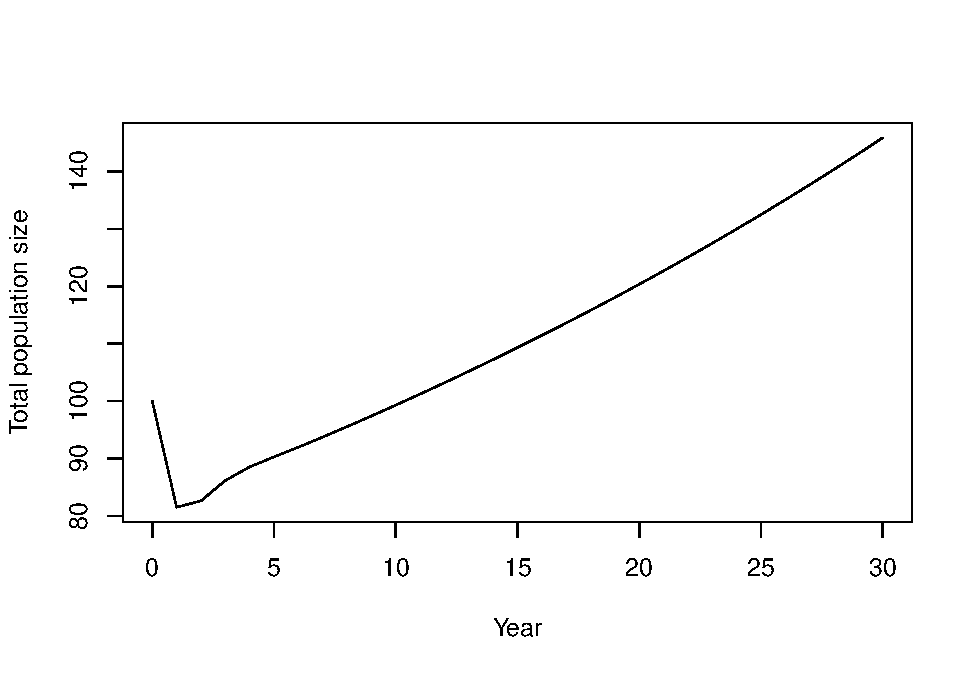
\includegraphics[keepaspectratio]{BB512_files/BB512_files/figure-latex/mpm_deterministic_plots-1.pdf}}

\begin{Shaded}
\begin{Highlighting}[]
\CommentTok{\# Plot stage{-}specific abundances}
\FunctionTok{matplot}\NormalTok{(}
  \DecValTok{0}\SpecialCharTok{:}\NormalTok{years, nmat, }\AttributeTok{type =} \StringTok{"l"}\NormalTok{, }\AttributeTok{lty =} \DecValTok{1}\NormalTok{,}
  \AttributeTok{xlab =} \StringTok{"Year"}\NormalTok{, }\AttributeTok{ylab =} \StringTok{"Abundance"}
\NormalTok{)}
\FunctionTok{legend}\NormalTok{(}\StringTok{"topleft"}\NormalTok{, }\AttributeTok{legend =} \FunctionTok{colnames}\NormalTok{(nmat), }\AttributeTok{lty =} \DecValTok{1}\NormalTok{, }\AttributeTok{bty =} \StringTok{"n"}\NormalTok{)}
\end{Highlighting}
\end{Shaded}

\pandocbounded{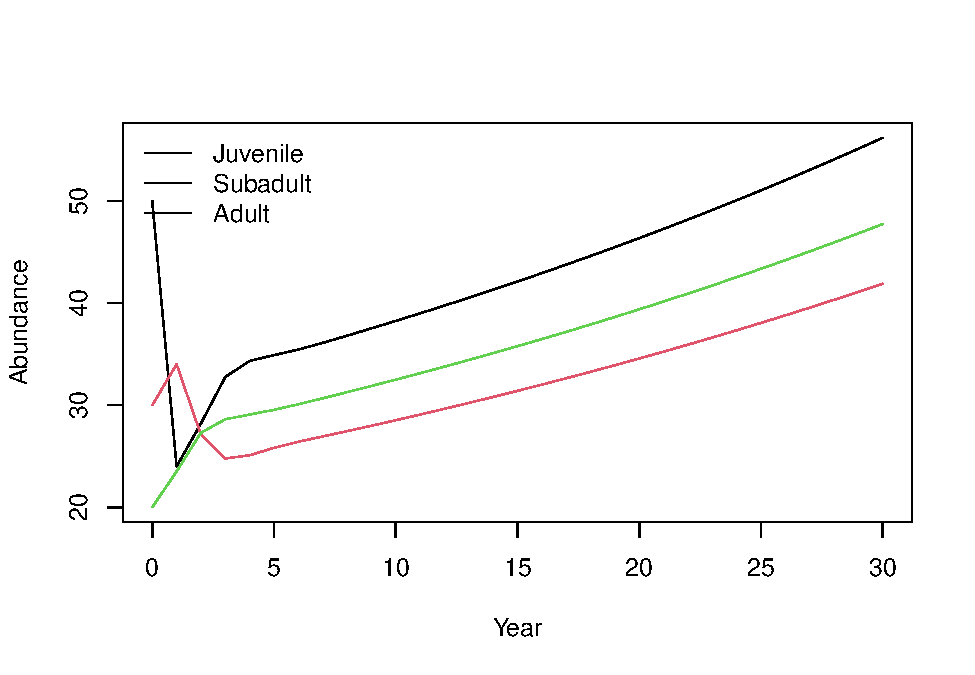
\includegraphics[keepaspectratio]{BB512_files/BB512_files/figure-latex/mpm_deterministic_plots-2.pdf}}

\section{Long-term growth rate (\textbackslash(\textbackslash lambda\textbackslash))}\label{long-term-growth-rate-lambda}

For a constant matrix \textbackslash(\textbackslash mathbf\{A\}\textbackslash), the asymptotic growth rate is the \textbf{dominant eigenvalue} \textbackslash(\textbackslash lambda\textbackslash).

\begin{Shaded}
\begin{Highlighting}[]
\CommentTok{\# Eigenvalues of the projection matrix}
\NormalTok{eig }\OtherTok{\textless{}{-}} \FunctionTok{eigen}\NormalTok{(A)}

\CommentTok{\# Dominant eigenvalue is asymptotic growth rate lambda}
\NormalTok{lambda }\OtherTok{\textless{}{-}} \FunctionTok{Re}\NormalTok{(eig}\SpecialCharTok{$}\NormalTok{values[}\FunctionTok{which.max}\NormalTok{(}\FunctionTok{Re}\NormalTok{(eig}\SpecialCharTok{$}\NormalTok{values))])}
\NormalTok{lambda}
\end{Highlighting}
\end{Shaded}

\begin{verbatim}
## [1] 1.01942
\end{verbatim}

\begin{itemize}
\tightlist
\item
  If \textbackslash(\textbackslash lambda \textgreater{} 1\textbackslash): growth (on average) per time step\\
\item
  If \textbackslash(\textbackslash lambda = 1\textbackslash): stationary\\
\item
  If \textbackslash(\textbackslash lambda \textless{} 1\textbackslash): decline
\end{itemize}

\section{Simulation: adding stochasticity and management actions}\label{simulation-adding-stochasticity-and-management-actions}

Deterministic projection treats the model output as exact expectations. In reality:

\begin{itemize}
\tightlist
\item
  births and deaths vary (demographic stochasticity),
\item
  vital rates vary across years (environmental stochasticity),
\item
  management can intervene (culling, supplementation, etc.).
\end{itemize}

Below is a transparent stochastic simulation that:

\begin{itemize}
\tightlist
\item
  simulates reproduction with Poisson variation,
\item
  simulates survival/transitions with binomial variation,
\item
  allows a simple \textbf{culling} intervention.
\end{itemize}

\subsection{One simulated trajectory (no culling)}\label{one-simulated-trajectory-no-culling}

Here we write the simulation as a sequence of explicit steps.

\begin{enumerate}
\def\labelenumi{\arabic{enumi}.}
\tightlist
\item
  Create an output matrix (\texttt{sim1}) with one row per year and one column per stage.
\item
  Fill row 1 with the initial stage abundances (\texttt{n0}).
\item
  For each year, read the current stage counts (\texttt{J}, \texttt{S}, \texttt{A}).
\item
  Draw the number of births and transitions using random distributions:

  \begin{itemize}
  \tightlist
  \item
    births from adults: Poisson
  \item
    survival/transition events: Binomial
  \end{itemize}
\item
  Write the resulting stage counts into the next row.
\item
  After the loop, plot total abundance through time.
\end{enumerate}

\begin{Shaded}
\begin{Highlighting}[]
\CommentTok{\# Step 1: create a matrix to store the trajectory}
\NormalTok{sim1 }\OtherTok{\textless{}{-}} \FunctionTok{matrix}\NormalTok{(}\DecValTok{0}\DataTypeTok{L}\NormalTok{, }\AttributeTok{nrow =}\NormalTok{ years }\SpecialCharTok{+} \DecValTok{1}\NormalTok{, }\AttributeTok{ncol =} \DecValTok{3}\NormalTok{)}
\FunctionTok{colnames}\NormalTok{(sim1) }\OtherTok{\textless{}{-}} \FunctionTok{c}\NormalTok{(}\StringTok{"Juvenile"}\NormalTok{, }\StringTok{"Subadult"}\NormalTok{, }\StringTok{"Adult"}\NormalTok{)}

\CommentTok{\# Step 2: set the initial population (year 0)}
\NormalTok{sim1[}\DecValTok{1}\NormalTok{, ] }\OtherTok{\textless{}{-}} \FunctionTok{as.integer}\NormalTok{(n0[}\FunctionTok{c}\NormalTok{(}\StringTok{"Juvenile"}\NormalTok{, }\StringTok{"Subadult"}\NormalTok{, }\StringTok{"Adult"}\NormalTok{)])}

\CommentTok{\# Step 3{-}5: update the population one year at a time}
\ControlFlowTok{for}\NormalTok{ (t }\ControlFlowTok{in} \DecValTok{1}\SpecialCharTok{:}\NormalTok{years) \{}
  \CommentTok{\# Current stage abundances at year t}
\NormalTok{  J }\OtherTok{\textless{}{-}}\NormalTok{ sim1[t, }\StringTok{"Juvenile"}\NormalTok{]}
\NormalTok{  S }\OtherTok{\textless{}{-}}\NormalTok{ sim1[t, }\StringTok{"Subadult"}\NormalTok{]}
\NormalTok{  A }\OtherTok{\textless{}{-}}\NormalTok{ sim1[t, }\StringTok{"Adult"}\NormalTok{]}

  \CommentTok{\# Births: each adult contributes recruits stochastically}
\NormalTok{  newJ }\OtherTok{\textless{}{-}} \FunctionTok{rpois}\NormalTok{(}\DecValTok{1}\NormalTok{, }\AttributeTok{lambda =}\NormalTok{ F\_A }\SpecialCharTok{*}\NormalTok{ A)}

  \CommentTok{\# Juvenile {-}\textgreater{} Subadult transition}
\NormalTok{  J\_to\_S }\OtherTok{\textless{}{-}} \FunctionTok{rbinom}\NormalTok{(}\DecValTok{1}\NormalTok{, }\AttributeTok{size =}\NormalTok{ J, }\AttributeTok{prob =}\NormalTok{ G\_J)}

  \CommentTok{\# Subadult transitions: stay subadult or move to adult}
\NormalTok{  S\_stay }\OtherTok{\textless{}{-}} \FunctionTok{rbinom}\NormalTok{(}\DecValTok{1}\NormalTok{, }\AttributeTok{size =}\NormalTok{ S, }\AttributeTok{prob =}\NormalTok{ P\_S)}
\NormalTok{  S\_remaining }\OtherTok{\textless{}{-}}\NormalTok{ S }\SpecialCharTok{{-}}\NormalTok{ S\_stay}
\NormalTok{  p\_grow\_cond }\OtherTok{\textless{}{-}} \ControlFlowTok{if}\NormalTok{ ((}\DecValTok{1} \SpecialCharTok{{-}}\NormalTok{ P\_S) }\SpecialCharTok{\textgreater{}} \DecValTok{0}\NormalTok{) G\_S }\SpecialCharTok{/}\NormalTok{ (}\DecValTok{1} \SpecialCharTok{{-}}\NormalTok{ P\_S) }\ControlFlowTok{else} \DecValTok{0}
\NormalTok{  S\_to\_A }\OtherTok{\textless{}{-}} \FunctionTok{rbinom}\NormalTok{(}\DecValTok{1}\NormalTok{, }\AttributeTok{size =}\NormalTok{ S\_remaining, }\AttributeTok{prob =}\NormalTok{ p\_grow\_cond)}

  \CommentTok{\# Adult survival}
\NormalTok{  A\_surv }\OtherTok{\textless{}{-}} \FunctionTok{rbinom}\NormalTok{(}\DecValTok{1}\NormalTok{, }\AttributeTok{size =}\NormalTok{ A, }\AttributeTok{prob =}\NormalTok{ P\_A)}

  \CommentTok{\# Write next year\textquotesingle{}s abundances}
\NormalTok{  sim1[t }\SpecialCharTok{+} \DecValTok{1}\NormalTok{, }\StringTok{"Juvenile"}\NormalTok{] }\OtherTok{\textless{}{-}}\NormalTok{ newJ}
\NormalTok{  sim1[t }\SpecialCharTok{+} \DecValTok{1}\NormalTok{, }\StringTok{"Subadult"}\NormalTok{] }\OtherTok{\textless{}{-}}\NormalTok{ J\_to\_S }\SpecialCharTok{+}\NormalTok{ S\_stay}
\NormalTok{  sim1[t }\SpecialCharTok{+} \DecValTok{1}\NormalTok{, }\StringTok{"Adult"}\NormalTok{] }\OtherTok{\textless{}{-}}\NormalTok{ S\_to\_A }\SpecialCharTok{+}\NormalTok{ A\_surv}
\NormalTok{\}}

\CommentTok{\# Step 6: plot the total population trajectory}
\FunctionTok{plot}\NormalTok{(}\DecValTok{0}\SpecialCharTok{:}\NormalTok{years, }\FunctionTok{rowSums}\NormalTok{(sim1), }\AttributeTok{type =} \StringTok{"l"}\NormalTok{,}
     \AttributeTok{xlab =} \StringTok{"Year"}\NormalTok{, }\AttributeTok{ylab =} \StringTok{"Total population size (simulated)"}\NormalTok{)}
\end{Highlighting}
\end{Shaded}

\pandocbounded{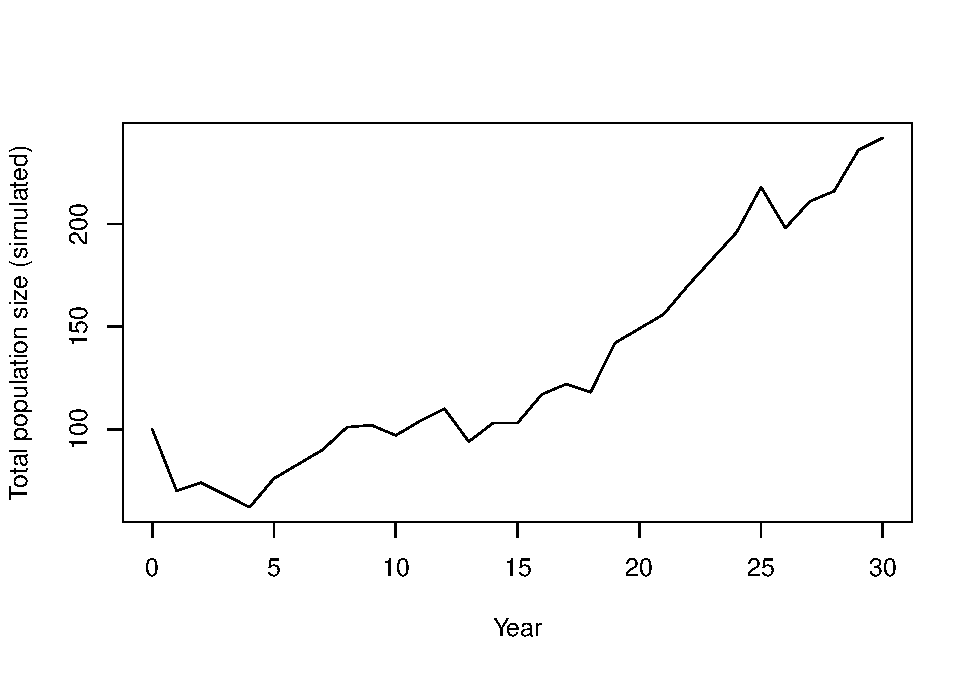
\includegraphics[keepaspectratio]{BB512_files/BB512_files/figure-latex/mpm_sim_no_cull-1.pdf}}

Just after running the simulation, we can calculate the realised \texttt{lambda} for this no-culling trajectory.

\begin{Shaded}
\begin{Highlighting}[]
\NormalTok{tot\_no }\OtherTok{\textless{}{-}} \FunctionTok{rowSums}\NormalTok{(sim1)}
\NormalTok{realised\_lambda\_no }\OtherTok{\textless{}{-}} \ControlFlowTok{if}\NormalTok{ (}\FunctionTok{length}\NormalTok{(tot\_no) }\SpecialCharTok{\textless{}} \DecValTok{2} \SpecialCharTok{||}\NormalTok{ tot\_no[}\DecValTok{1}\NormalTok{] }\SpecialCharTok{\textless{}=} \DecValTok{0}\NormalTok{) \{}
  \ConstantTok{NA\_real\_}
\NormalTok{\} }\ControlFlowTok{else} \ControlFlowTok{if}\NormalTok{ (}\FunctionTok{any}\NormalTok{(tot\_no }\SpecialCharTok{\textless{}=} \DecValTok{0}\NormalTok{)) \{}
  \DecValTok{0}
\NormalTok{\} }\ControlFlowTok{else}\NormalTok{ \{}
  \FunctionTok{exp}\NormalTok{(}\FunctionTok{mean}\NormalTok{(}\FunctionTok{diff}\NormalTok{(}\FunctionTok{log}\NormalTok{(tot\_no))))}
\NormalTok{\}}
\NormalTok{realised\_lambda\_no}
\end{Highlighting}
\end{Shaded}

\begin{verbatim}
## [1] 1.029897
\end{verbatim}

\subsection{Add a culling intervention}\label{add-a-culling-intervention}

Example: remove 5 adults per year starting at year 10.
This section uses the same simulation rules as before, but adds a management step at the start of each year.

What happens:

\begin{enumerate}
\def\labelenumi{\arabic{enumi}.}
\tightlist
\item
  Scenario A (no culling) was simulated in the previous section and stored as \texttt{sim1}.
\item
  We set intervention controls (\texttt{cull\_enabled}, \texttt{cull\_stage}, \texttt{cull\_start\_year}, \texttt{cull\_n}) for Scenario B.
\item
  At each year \texttt{t}, we first read current stage abundances (\texttt{J}, \texttt{S}, \texttt{A}).
\item
  If culling is active and \texttt{t} is at/after the start year, we remove individuals from the target stage.
\item
  We then refresh \texttt{J}, \texttt{S}, \texttt{A} so births and survival are based on the post-cull population.
\item
  After that, demographic updates are exactly the same as in Scenario A.
\item
  Finally, we compare Scenario A and B in one figure and compute realised growth rates.
\end{enumerate}

\begin{Shaded}
\begin{Highlighting}[]
\CommentTok{\# Management settings for the intervention scenario}
\NormalTok{cull\_enabled }\OtherTok{\textless{}{-}} \ConstantTok{TRUE}
\NormalTok{cull\_stage }\OtherTok{\textless{}{-}} \StringTok{"Adult"}
\NormalTok{cull\_start\_year }\OtherTok{\textless{}{-}} \DecValTok{10}
\NormalTok{cull\_n }\OtherTok{\textless{}{-}} \DecValTok{5}

\CommentTok{\# Storage for the culling trajectory}
\NormalTok{sim\_cull }\OtherTok{\textless{}{-}} \FunctionTok{matrix}\NormalTok{(}\DecValTok{0}\DataTypeTok{L}\NormalTok{, }\AttributeTok{nrow =}\NormalTok{ years }\SpecialCharTok{+} \DecValTok{1}\NormalTok{, }\AttributeTok{ncol =} \DecValTok{3}\NormalTok{)}
\FunctionTok{colnames}\NormalTok{(sim\_cull) }\OtherTok{\textless{}{-}} \FunctionTok{c}\NormalTok{(}\StringTok{"Juvenile"}\NormalTok{, }\StringTok{"Subadult"}\NormalTok{, }\StringTok{"Adult"}\NormalTok{)}
\NormalTok{sim\_cull[}\DecValTok{1}\NormalTok{, ] }\OtherTok{\textless{}{-}} \FunctionTok{as.integer}\NormalTok{(n0[}\FunctionTok{c}\NormalTok{(}\StringTok{"Juvenile"}\NormalTok{, }\StringTok{"Subadult"}\NormalTok{, }\StringTok{"Adult"}\NormalTok{)])}

\CommentTok{\# Simulate year by year, applying culling before demographic updates}
\ControlFlowTok{for}\NormalTok{ (t }\ControlFlowTok{in} \DecValTok{1}\SpecialCharTok{:}\NormalTok{years) \{}
  \CommentTok{\# Current stage abundances at year t}
\NormalTok{  J }\OtherTok{\textless{}{-}}\NormalTok{ sim\_cull[t, }\StringTok{"Juvenile"}\NormalTok{]}
\NormalTok{  S }\OtherTok{\textless{}{-}}\NormalTok{ sim\_cull[t, }\StringTok{"Subadult"}\NormalTok{]}
\NormalTok{  A }\OtherTok{\textless{}{-}}\NormalTok{ sim\_cull[t, }\StringTok{"Adult"}\NormalTok{]}

  \CommentTok{\# Apply culling before births/survival if intervention is active}
  \ControlFlowTok{if}\NormalTok{ (cull\_enabled }\SpecialCharTok{\&\&}\NormalTok{ t }\SpecialCharTok{\textgreater{}=}\NormalTok{ cull\_start\_year) \{}
    \CommentTok{\# Never remove more individuals than are currently present}
\NormalTok{    remove\_n }\OtherTok{\textless{}{-}} \FunctionTok{min}\NormalTok{(sim\_cull[t, cull\_stage], }\FunctionTok{as.integer}\NormalTok{(cull\_n))}
\NormalTok{    sim\_cull[t, cull\_stage] }\OtherTok{\textless{}{-}}\NormalTok{ sim\_cull[t, cull\_stage] }\SpecialCharTok{{-}}\NormalTok{ remove\_n}

    \CommentTok{\# Refresh stage counts after culling}
\NormalTok{    J }\OtherTok{\textless{}{-}}\NormalTok{ sim\_cull[t, }\StringTok{"Juvenile"}\NormalTok{]}
\NormalTok{    S }\OtherTok{\textless{}{-}}\NormalTok{ sim\_cull[t, }\StringTok{"Subadult"}\NormalTok{]}
\NormalTok{    A }\OtherTok{\textless{}{-}}\NormalTok{ sim\_cull[t, }\StringTok{"Adult"}\NormalTok{]}
\NormalTok{  \}}

  \CommentTok{\# Demographic updates (same as the no{-}culling simulation)}
\NormalTok{  newJ }\OtherTok{\textless{}{-}} \FunctionTok{rpois}\NormalTok{(}\DecValTok{1}\NormalTok{, }\AttributeTok{lambda =}\NormalTok{ F\_A }\SpecialCharTok{*}\NormalTok{ A)}
\NormalTok{  J\_to\_S }\OtherTok{\textless{}{-}} \FunctionTok{rbinom}\NormalTok{(}\DecValTok{1}\NormalTok{, }\AttributeTok{size =}\NormalTok{ J, }\AttributeTok{prob =}\NormalTok{ G\_J)}
\NormalTok{  S\_stay }\OtherTok{\textless{}{-}} \FunctionTok{rbinom}\NormalTok{(}\DecValTok{1}\NormalTok{, }\AttributeTok{size =}\NormalTok{ S, }\AttributeTok{prob =}\NormalTok{ P\_S)}
\NormalTok{  S\_remaining }\OtherTok{\textless{}{-}}\NormalTok{ S }\SpecialCharTok{{-}}\NormalTok{ S\_stay}
\NormalTok{  p\_grow\_cond }\OtherTok{\textless{}{-}} \ControlFlowTok{if}\NormalTok{ ((}\DecValTok{1} \SpecialCharTok{{-}}\NormalTok{ P\_S) }\SpecialCharTok{\textgreater{}} \DecValTok{0}\NormalTok{) G\_S }\SpecialCharTok{/}\NormalTok{ (}\DecValTok{1} \SpecialCharTok{{-}}\NormalTok{ P\_S) }\ControlFlowTok{else} \DecValTok{0}
\NormalTok{  S\_to\_A }\OtherTok{\textless{}{-}} \FunctionTok{rbinom}\NormalTok{(}\DecValTok{1}\NormalTok{, }\AttributeTok{size =}\NormalTok{ S\_remaining, }\AttributeTok{prob =}\NormalTok{ p\_grow\_cond)}
\NormalTok{  A\_surv }\OtherTok{\textless{}{-}} \FunctionTok{rbinom}\NormalTok{(}\DecValTok{1}\NormalTok{, }\AttributeTok{size =}\NormalTok{ A, }\AttributeTok{prob =}\NormalTok{ P\_A)}

\NormalTok{  sim\_cull[t }\SpecialCharTok{+} \DecValTok{1}\NormalTok{, }\StringTok{"Juvenile"}\NormalTok{] }\OtherTok{\textless{}{-}}\NormalTok{ newJ}
\NormalTok{  sim\_cull[t }\SpecialCharTok{+} \DecValTok{1}\NormalTok{, }\StringTok{"Subadult"}\NormalTok{] }\OtherTok{\textless{}{-}}\NormalTok{ J\_to\_S }\SpecialCharTok{+}\NormalTok{ S\_stay}
\NormalTok{  sim\_cull[t }\SpecialCharTok{+} \DecValTok{1}\NormalTok{, }\StringTok{"Adult"}\NormalTok{] }\OtherTok{\textless{}{-}}\NormalTok{ S\_to\_A }\SpecialCharTok{+}\NormalTok{ A\_surv}
\NormalTok{\}}

\CommentTok{\# Compare trajectories: solid = no culling, dashed = culling}
\FunctionTok{plot}\NormalTok{(}\DecValTok{0}\SpecialCharTok{:}\NormalTok{years, }\FunctionTok{rowSums}\NormalTok{(sim1), }\AttributeTok{type =} \StringTok{"l"}\NormalTok{,}
     \AttributeTok{xlab =} \StringTok{"Year"}\NormalTok{, }\AttributeTok{ylab =} \StringTok{"Total population size"}\NormalTok{,}
     \AttributeTok{ylim =} \FunctionTok{range}\NormalTok{(}\FunctionTok{c}\NormalTok{(}\FunctionTok{rowSums}\NormalTok{(sim1), }\FunctionTok{rowSums}\NormalTok{(sim\_cull))))}
\FunctionTok{lines}\NormalTok{(}\DecValTok{0}\SpecialCharTok{:}\NormalTok{years, }\FunctionTok{rowSums}\NormalTok{(sim\_cull), }\AttributeTok{lty =} \DecValTok{2}\NormalTok{)}
\FunctionTok{legend}\NormalTok{(}\StringTok{"topleft"}\NormalTok{, }\AttributeTok{legend =} \FunctionTok{c}\NormalTok{(}\StringTok{"No culling"}\NormalTok{, }\StringTok{"Culling: 5 adults/year from year 10"}\NormalTok{),}
       \AttributeTok{lty =} \FunctionTok{c}\NormalTok{(}\DecValTok{1}\NormalTok{, }\DecValTok{2}\NormalTok{), }\AttributeTok{bty =} \StringTok{"n"}\NormalTok{)}
\end{Highlighting}
\end{Shaded}

\pandocbounded{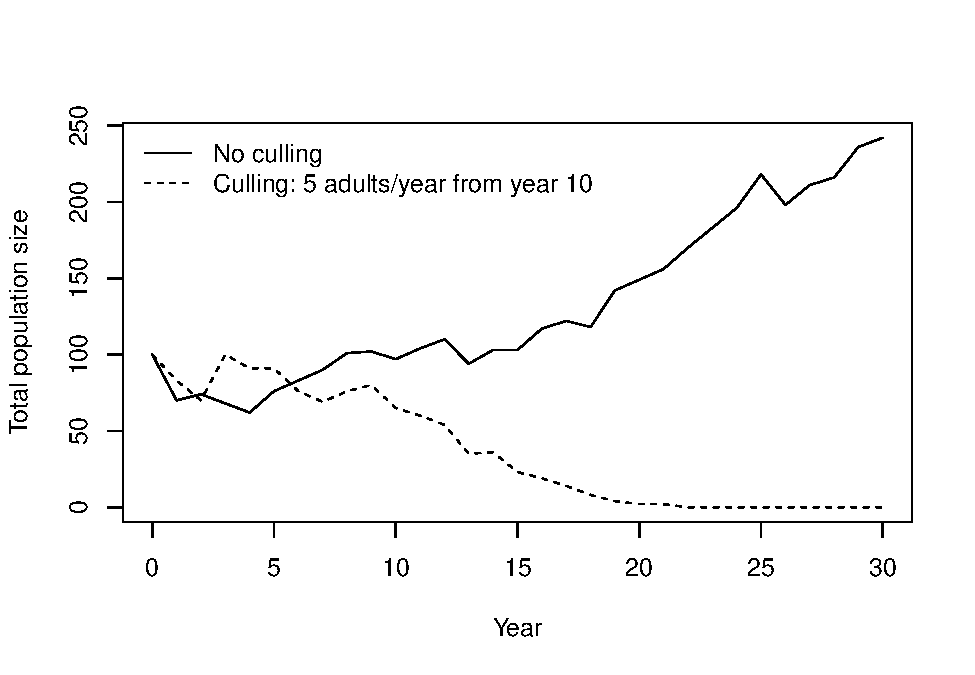
\includegraphics[keepaspectratio]{BB512_files/BB512_files/figure-latex/mpm_sim_with_cull-1.pdf}}

For this single-run summary, realised \texttt{lambda} is the geometric mean of year-to-year total-population growth factors. This is a finite-horizon, trajectory-specific estimate; in many ecology texts, the long-run stochastic growth rate is denoted \textbackslash(\textbackslash lambda\_s\textbackslash) (or \textbackslash(\textbackslash log \textbackslash lambda\_s\textbackslash)), which is related but not identical to a single-run realised value.

Interpretation:

\begin{itemize}
\tightlist
\item
  \texttt{lambda\ \textgreater{}\ 1}: realised growth over the simulated period
\item
  \texttt{0\ \textless{}\ lambda\ \textless{}\ 1}: realised decline
\item
  \texttt{lambda\ =\ 0}: extinction occurred at some point in the simulated period
\item
  \texttt{lambda} should not be negative in this setting
\end{itemize}

\begin{Shaded}
\begin{Highlighting}[]
\CommentTok{\# Realised lambda from each simulated trajectory}
\NormalTok{tot\_no }\OtherTok{\textless{}{-}} \FunctionTok{rowSums}\NormalTok{(sim1)}
\NormalTok{tot\_cu }\OtherTok{\textless{}{-}} \FunctionTok{rowSums}\NormalTok{(sim\_cull)}

\CommentTok{\# Geometric{-}mean per{-}step growth rate over the full horizon.}
\CommentTok{\# If a trajectory hits zero, define realised lambda as 0 (extinction within horizon).}
\NormalTok{realised\_lambda\_no }\OtherTok{\textless{}{-}} \ControlFlowTok{if}\NormalTok{ (}\FunctionTok{length}\NormalTok{(tot\_no) }\SpecialCharTok{\textless{}} \DecValTok{2} \SpecialCharTok{||}\NormalTok{ tot\_no[}\DecValTok{1}\NormalTok{] }\SpecialCharTok{\textless{}=} \DecValTok{0}\NormalTok{) \{}
  \ConstantTok{NA\_real\_}
\NormalTok{\} }\ControlFlowTok{else} \ControlFlowTok{if}\NormalTok{ (}\FunctionTok{any}\NormalTok{(tot\_no }\SpecialCharTok{\textless{}=} \DecValTok{0}\NormalTok{)) \{}
  \DecValTok{0}
\NormalTok{\} }\ControlFlowTok{else}\NormalTok{ \{}
  \FunctionTok{exp}\NormalTok{(}\FunctionTok{mean}\NormalTok{(}\FunctionTok{diff}\NormalTok{(}\FunctionTok{log}\NormalTok{(tot\_no))))}
\NormalTok{\}}

\NormalTok{realised\_lambda\_cu }\OtherTok{\textless{}{-}} \ControlFlowTok{if}\NormalTok{ (}\FunctionTok{length}\NormalTok{(tot\_cu) }\SpecialCharTok{\textless{}} \DecValTok{2} \SpecialCharTok{||}\NormalTok{ tot\_cu[}\DecValTok{1}\NormalTok{] }\SpecialCharTok{\textless{}=} \DecValTok{0}\NormalTok{) \{}
  \ConstantTok{NA\_real\_}
\NormalTok{\} }\ControlFlowTok{else} \ControlFlowTok{if}\NormalTok{ (}\FunctionTok{any}\NormalTok{(tot\_cu }\SpecialCharTok{\textless{}=} \DecValTok{0}\NormalTok{)) \{}
  \DecValTok{0}
\NormalTok{\} }\ControlFlowTok{else}\NormalTok{ \{}
  \FunctionTok{exp}\NormalTok{(}\FunctionTok{mean}\NormalTok{(}\FunctionTok{diff}\NormalTok{(}\FunctionTok{log}\NormalTok{(tot\_cu))))}
\NormalTok{\}}

\FunctionTok{data.frame}\NormalTok{(}
  \AttributeTok{scenario =} \FunctionTok{c}\NormalTok{(}\StringTok{"No culling"}\NormalTok{, }\StringTok{"Culling"}\NormalTok{),}
  \AttributeTok{realised\_lambda =} \FunctionTok{c}\NormalTok{(realised\_lambda\_no, realised\_lambda\_cu)}
\NormalTok{)}
\end{Highlighting}
\end{Shaded}

\begin{verbatim}
##     scenario realised_lambda
## 1 No culling        1.029897
## 2    Culling        0.000000
\end{verbatim}

\subsection{Many replicates (uncertainty bands)}\label{many-replicates-uncertainty-bands}

A single run is one possible realisation. We typically run many replicates and summarise.
In this script, we run two sets of replicates (no culling vs culling), then compute median and 10-90\% intervals for each year.
Note: different studies may use different interval widths (for example, 95\% intervals) depending on purpose and reporting conventions.
To keep the comparison clear, the code is structured as:
1. Scenario A: run all replicates with no culling.
2. Scenario B: run all replicates with culling.
3. Compare Scenario A and B in one graph.

\begin{Shaded}
\begin{Highlighting}[]
\CommentTok{\# Number of Monte Carlo replicates}
\NormalTok{nreps }\OtherTok{\textless{}{-}} \DecValTok{200}

\CommentTok{\# Store total abundance per year for each replicate}
\NormalTok{totals\_no }\OtherTok{\textless{}{-}} \FunctionTok{matrix}\NormalTok{(}\ConstantTok{NA\_real\_}\NormalTok{, }\AttributeTok{nrow =}\NormalTok{ years }\SpecialCharTok{+} \DecValTok{1}\NormalTok{, }\AttributeTok{ncol =}\NormalTok{ nreps)}
\NormalTok{totals\_cull }\OtherTok{\textless{}{-}} \FunctionTok{matrix}\NormalTok{(}\ConstantTok{NA\_real\_}\NormalTok{, }\AttributeTok{nrow =}\NormalTok{ years }\SpecialCharTok{+} \DecValTok{1}\NormalTok{, }\AttributeTok{ncol =}\NormalTok{ nreps)}

\CommentTok{\# Scenario A: run all replicates with no culling}
\ControlFlowTok{for}\NormalTok{ (rep }\ControlFlowTok{in} \DecValTok{1}\SpecialCharTok{:}\NormalTok{nreps) \{}
\NormalTok{  out\_no }\OtherTok{\textless{}{-}} \FunctionTok{matrix}\NormalTok{(}\DecValTok{0}\DataTypeTok{L}\NormalTok{, }\AttributeTok{nrow =}\NormalTok{ years }\SpecialCharTok{+} \DecValTok{1}\NormalTok{, }\AttributeTok{ncol =} \DecValTok{3}\NormalTok{)}
  \FunctionTok{colnames}\NormalTok{(out\_no) }\OtherTok{\textless{}{-}} \FunctionTok{c}\NormalTok{(}\StringTok{"Juvenile"}\NormalTok{, }\StringTok{"Subadult"}\NormalTok{, }\StringTok{"Adult"}\NormalTok{)}
\NormalTok{  out\_no[}\DecValTok{1}\NormalTok{, ] }\OtherTok{\textless{}{-}} \FunctionTok{as.integer}\NormalTok{(n0[}\FunctionTok{c}\NormalTok{(}\StringTok{"Juvenile"}\NormalTok{, }\StringTok{"Subadult"}\NormalTok{, }\StringTok{"Adult"}\NormalTok{)])}

  \ControlFlowTok{for}\NormalTok{ (t }\ControlFlowTok{in} \DecValTok{1}\SpecialCharTok{:}\NormalTok{years) \{}
\NormalTok{    J }\OtherTok{\textless{}{-}}\NormalTok{ out\_no[t, }\StringTok{"Juvenile"}\NormalTok{]}
\NormalTok{    S }\OtherTok{\textless{}{-}}\NormalTok{ out\_no[t, }\StringTok{"Subadult"}\NormalTok{]}
\NormalTok{    A }\OtherTok{\textless{}{-}}\NormalTok{ out\_no[t, }\StringTok{"Adult"}\NormalTok{]}

\NormalTok{    newJ }\OtherTok{\textless{}{-}} \FunctionTok{rpois}\NormalTok{(}\DecValTok{1}\NormalTok{, }\AttributeTok{lambda =}\NormalTok{ F\_A }\SpecialCharTok{*}\NormalTok{ A)}
\NormalTok{    J\_to\_S }\OtherTok{\textless{}{-}} \FunctionTok{rbinom}\NormalTok{(}\DecValTok{1}\NormalTok{, }\AttributeTok{size =}\NormalTok{ J, }\AttributeTok{prob =}\NormalTok{ G\_J)}
\NormalTok{    S\_stay }\OtherTok{\textless{}{-}} \FunctionTok{rbinom}\NormalTok{(}\DecValTok{1}\NormalTok{, }\AttributeTok{size =}\NormalTok{ S, }\AttributeTok{prob =}\NormalTok{ P\_S)}
\NormalTok{    S\_remaining }\OtherTok{\textless{}{-}}\NormalTok{ S }\SpecialCharTok{{-}}\NormalTok{ S\_stay}
\NormalTok{    p\_grow\_cond }\OtherTok{\textless{}{-}} \ControlFlowTok{if}\NormalTok{ ((}\DecValTok{1} \SpecialCharTok{{-}}\NormalTok{ P\_S) }\SpecialCharTok{\textgreater{}} \DecValTok{0}\NormalTok{) G\_S }\SpecialCharTok{/}\NormalTok{ (}\DecValTok{1} \SpecialCharTok{{-}}\NormalTok{ P\_S) }\ControlFlowTok{else} \DecValTok{0}
\NormalTok{    S\_to\_A }\OtherTok{\textless{}{-}} \FunctionTok{rbinom}\NormalTok{(}\DecValTok{1}\NormalTok{, }\AttributeTok{size =}\NormalTok{ S\_remaining, }\AttributeTok{prob =}\NormalTok{ p\_grow\_cond)}
\NormalTok{    A\_surv }\OtherTok{\textless{}{-}} \FunctionTok{rbinom}\NormalTok{(}\DecValTok{1}\NormalTok{, }\AttributeTok{size =}\NormalTok{ A, }\AttributeTok{prob =}\NormalTok{ P\_A)}

\NormalTok{    out\_no[t }\SpecialCharTok{+} \DecValTok{1}\NormalTok{, }\StringTok{"Juvenile"}\NormalTok{] }\OtherTok{\textless{}{-}}\NormalTok{ newJ}
\NormalTok{    out\_no[t }\SpecialCharTok{+} \DecValTok{1}\NormalTok{, }\StringTok{"Subadult"}\NormalTok{] }\OtherTok{\textless{}{-}}\NormalTok{ J\_to\_S }\SpecialCharTok{+}\NormalTok{ S\_stay}
\NormalTok{    out\_no[t }\SpecialCharTok{+} \DecValTok{1}\NormalTok{, }\StringTok{"Adult"}\NormalTok{] }\OtherTok{\textless{}{-}}\NormalTok{ S\_to\_A }\SpecialCharTok{+}\NormalTok{ A\_surv}
\NormalTok{  \}}
\NormalTok{  totals\_no[, rep] }\OtherTok{\textless{}{-}} \FunctionTok{rowSums}\NormalTok{(out\_no)}
\NormalTok{\}}
\end{Highlighting}
\end{Shaded}

\begin{Shaded}
\begin{Highlighting}[]
\CommentTok{\# Scenario B: run all replicates with culling}
\ControlFlowTok{for}\NormalTok{ (rep }\ControlFlowTok{in} \DecValTok{1}\SpecialCharTok{:}\NormalTok{nreps) \{}
\NormalTok{  out\_cu }\OtherTok{\textless{}{-}} \FunctionTok{matrix}\NormalTok{(}\DecValTok{0}\DataTypeTok{L}\NormalTok{, }\AttributeTok{nrow =}\NormalTok{ years }\SpecialCharTok{+} \DecValTok{1}\NormalTok{, }\AttributeTok{ncol =} \DecValTok{3}\NormalTok{)}
  \FunctionTok{colnames}\NormalTok{(out\_cu) }\OtherTok{\textless{}{-}} \FunctionTok{c}\NormalTok{(}\StringTok{"Juvenile"}\NormalTok{, }\StringTok{"Subadult"}\NormalTok{, }\StringTok{"Adult"}\NormalTok{)}
\NormalTok{  out\_cu[}\DecValTok{1}\NormalTok{, ] }\OtherTok{\textless{}{-}} \FunctionTok{as.integer}\NormalTok{(n0[}\FunctionTok{c}\NormalTok{(}\StringTok{"Juvenile"}\NormalTok{, }\StringTok{"Subadult"}\NormalTok{, }\StringTok{"Adult"}\NormalTok{)])}

  \ControlFlowTok{for}\NormalTok{ (t }\ControlFlowTok{in} \DecValTok{1}\SpecialCharTok{:}\NormalTok{years) \{}
\NormalTok{    J }\OtherTok{\textless{}{-}}\NormalTok{ out\_cu[t, }\StringTok{"Juvenile"}\NormalTok{]}
\NormalTok{    S }\OtherTok{\textless{}{-}}\NormalTok{ out\_cu[t, }\StringTok{"Subadult"}\NormalTok{]}
\NormalTok{    A }\OtherTok{\textless{}{-}}\NormalTok{ out\_cu[t, }\StringTok{"Adult"}\NormalTok{]}

    \ControlFlowTok{if}\NormalTok{ (cull\_enabled }\SpecialCharTok{\&\&}\NormalTok{ t }\SpecialCharTok{\textgreater{}=}\NormalTok{ cull\_start\_year) \{}
\NormalTok{      remove\_n }\OtherTok{\textless{}{-}} \FunctionTok{min}\NormalTok{(out\_cu[t, cull\_stage], }\FunctionTok{as.integer}\NormalTok{(cull\_n))}
\NormalTok{      out\_cu[t, cull\_stage] }\OtherTok{\textless{}{-}}\NormalTok{ out\_cu[t, cull\_stage] }\SpecialCharTok{{-}}\NormalTok{ remove\_n}
\NormalTok{      J }\OtherTok{\textless{}{-}}\NormalTok{ out\_cu[t, }\StringTok{"Juvenile"}\NormalTok{]}
\NormalTok{      S }\OtherTok{\textless{}{-}}\NormalTok{ out\_cu[t, }\StringTok{"Subadult"}\NormalTok{]}
\NormalTok{      A }\OtherTok{\textless{}{-}}\NormalTok{ out\_cu[t, }\StringTok{"Adult"}\NormalTok{]}
\NormalTok{    \}}

\NormalTok{    newJ }\OtherTok{\textless{}{-}} \FunctionTok{rpois}\NormalTok{(}\DecValTok{1}\NormalTok{, }\AttributeTok{lambda =}\NormalTok{ F\_A }\SpecialCharTok{*}\NormalTok{ A)}
\NormalTok{    J\_to\_S }\OtherTok{\textless{}{-}} \FunctionTok{rbinom}\NormalTok{(}\DecValTok{1}\NormalTok{, }\AttributeTok{size =}\NormalTok{ J, }\AttributeTok{prob =}\NormalTok{ G\_J)}
\NormalTok{    S\_stay }\OtherTok{\textless{}{-}} \FunctionTok{rbinom}\NormalTok{(}\DecValTok{1}\NormalTok{, }\AttributeTok{size =}\NormalTok{ S, }\AttributeTok{prob =}\NormalTok{ P\_S)}
\NormalTok{    S\_remaining }\OtherTok{\textless{}{-}}\NormalTok{ S }\SpecialCharTok{{-}}\NormalTok{ S\_stay}
\NormalTok{    p\_grow\_cond }\OtherTok{\textless{}{-}} \ControlFlowTok{if}\NormalTok{ ((}\DecValTok{1} \SpecialCharTok{{-}}\NormalTok{ P\_S) }\SpecialCharTok{\textgreater{}} \DecValTok{0}\NormalTok{) G\_S }\SpecialCharTok{/}\NormalTok{ (}\DecValTok{1} \SpecialCharTok{{-}}\NormalTok{ P\_S) }\ControlFlowTok{else} \DecValTok{0}
\NormalTok{    S\_to\_A }\OtherTok{\textless{}{-}} \FunctionTok{rbinom}\NormalTok{(}\DecValTok{1}\NormalTok{, }\AttributeTok{size =}\NormalTok{ S\_remaining, }\AttributeTok{prob =}\NormalTok{ p\_grow\_cond)}
\NormalTok{    A\_surv }\OtherTok{\textless{}{-}} \FunctionTok{rbinom}\NormalTok{(}\DecValTok{1}\NormalTok{, }\AttributeTok{size =}\NormalTok{ A, }\AttributeTok{prob =}\NormalTok{ P\_A)}

\NormalTok{    out\_cu[t }\SpecialCharTok{+} \DecValTok{1}\NormalTok{, }\StringTok{"Juvenile"}\NormalTok{] }\OtherTok{\textless{}{-}}\NormalTok{ newJ}
\NormalTok{    out\_cu[t }\SpecialCharTok{+} \DecValTok{1}\NormalTok{, }\StringTok{"Subadult"}\NormalTok{] }\OtherTok{\textless{}{-}}\NormalTok{ J\_to\_S }\SpecialCharTok{+}\NormalTok{ S\_stay}
\NormalTok{    out\_cu[t }\SpecialCharTok{+} \DecValTok{1}\NormalTok{, }\StringTok{"Adult"}\NormalTok{] }\OtherTok{\textless{}{-}}\NormalTok{ S\_to\_A }\SpecialCharTok{+}\NormalTok{ A\_surv}
\NormalTok{  \}}
\NormalTok{  totals\_cull[, rep] }\OtherTok{\textless{}{-}} \FunctionTok{rowSums}\NormalTok{(out\_cu)}
\NormalTok{\}}

\CommentTok{\# Summarise each year across replicates (median and 10{-}90\% interval)}
\NormalTok{sum\_no }\OtherTok{\textless{}{-}} \FunctionTok{data.frame}\NormalTok{(}
  \AttributeTok{year =} \DecValTok{0}\SpecialCharTok{:}\NormalTok{years,}
  \AttributeTok{median =} \FunctionTok{apply}\NormalTok{(totals\_no, }\DecValTok{1}\NormalTok{, median),}
  \AttributeTok{lo =} \FunctionTok{apply}\NormalTok{(totals\_no, }\DecValTok{1}\NormalTok{, quantile, }\AttributeTok{probs =} \FloatTok{0.1}\NormalTok{),}
  \AttributeTok{hi =} \FunctionTok{apply}\NormalTok{(totals\_no, }\DecValTok{1}\NormalTok{, quantile, }\AttributeTok{probs =} \FloatTok{0.9}\NormalTok{)}
\NormalTok{)}
\NormalTok{sum\_cu }\OtherTok{\textless{}{-}} \FunctionTok{data.frame}\NormalTok{(}
  \AttributeTok{year =} \DecValTok{0}\SpecialCharTok{:}\NormalTok{years,}
  \AttributeTok{median =} \FunctionTok{apply}\NormalTok{(totals\_cull, }\DecValTok{1}\NormalTok{, median),}
  \AttributeTok{lo =} \FunctionTok{apply}\NormalTok{(totals\_cull, }\DecValTok{1}\NormalTok{, quantile, }\AttributeTok{probs =} \FloatTok{0.1}\NormalTok{),}
  \AttributeTok{hi =} \FunctionTok{apply}\NormalTok{(totals\_cull, }\DecValTok{1}\NormalTok{, quantile, }\AttributeTok{probs =} \FloatTok{0.9}\NormalTok{)}
\NormalTok{)}

\CommentTok{\# Scenario A vs Scenario B: compare summaries in one figure}
\FunctionTok{plot}\NormalTok{(sum\_no}\SpecialCharTok{$}\NormalTok{year, sum\_no}\SpecialCharTok{$}\NormalTok{median, }\AttributeTok{type =} \StringTok{"n"}\NormalTok{,}
     \AttributeTok{xlab =} \StringTok{"Year"}\NormalTok{, }\AttributeTok{ylab =} \StringTok{"Total population size"}\NormalTok{,}
     \AttributeTok{ylim =} \FunctionTok{range}\NormalTok{(}\FunctionTok{c}\NormalTok{(sum\_no}\SpecialCharTok{$}\NormalTok{lo, sum\_no}\SpecialCharTok{$}\NormalTok{hi, sum\_cu}\SpecialCharTok{$}\NormalTok{lo, sum\_cu}\SpecialCharTok{$}\NormalTok{hi)))}

\CommentTok{\# Ribbon for no{-}culling uncertainty (10{-}90\%)}
\FunctionTok{polygon}\NormalTok{(}
  \AttributeTok{x =} \FunctionTok{c}\NormalTok{(sum\_no}\SpecialCharTok{$}\NormalTok{year, }\FunctionTok{rev}\NormalTok{(sum\_no}\SpecialCharTok{$}\NormalTok{year)),}
  \AttributeTok{y =} \FunctionTok{c}\NormalTok{(sum\_no}\SpecialCharTok{$}\NormalTok{lo, }\FunctionTok{rev}\NormalTok{(sum\_no}\SpecialCharTok{$}\NormalTok{hi)),}
  \AttributeTok{col =}\NormalTok{ grDevices}\SpecialCharTok{::}\FunctionTok{adjustcolor}\NormalTok{(}\StringTok{"steelblue"}\NormalTok{, }\AttributeTok{alpha.f =} \FloatTok{0.25}\NormalTok{),}
  \AttributeTok{border =} \ConstantTok{NA}
\NormalTok{)}

\CommentTok{\# Ribbon for culling uncertainty (10{-}90\%)}
\FunctionTok{polygon}\NormalTok{(}
  \AttributeTok{x =} \FunctionTok{c}\NormalTok{(sum\_cu}\SpecialCharTok{$}\NormalTok{year, }\FunctionTok{rev}\NormalTok{(sum\_cu}\SpecialCharTok{$}\NormalTok{year)),}
  \AttributeTok{y =} \FunctionTok{c}\NormalTok{(sum\_cu}\SpecialCharTok{$}\NormalTok{lo, }\FunctionTok{rev}\NormalTok{(sum\_cu}\SpecialCharTok{$}\NormalTok{hi)),}
  \AttributeTok{col =}\NormalTok{ grDevices}\SpecialCharTok{::}\FunctionTok{adjustcolor}\NormalTok{(}\StringTok{"firebrick"}\NormalTok{, }\AttributeTok{alpha.f =} \FloatTok{0.25}\NormalTok{),}
  \AttributeTok{border =} \ConstantTok{NA}
\NormalTok{)}

\CommentTok{\# Median trajectories on top of ribbons}
\FunctionTok{lines}\NormalTok{(sum\_no}\SpecialCharTok{$}\NormalTok{year, sum\_no}\SpecialCharTok{$}\NormalTok{median, }\AttributeTok{lwd =} \DecValTok{2}\NormalTok{, }\AttributeTok{col =} \StringTok{"steelblue4"}\NormalTok{)}
\FunctionTok{lines}\NormalTok{(sum\_cu}\SpecialCharTok{$}\NormalTok{year, sum\_cu}\SpecialCharTok{$}\NormalTok{median, }\AttributeTok{lwd =} \DecValTok{2}\NormalTok{, }\AttributeTok{lty =} \DecValTok{2}\NormalTok{, }\AttributeTok{col =} \StringTok{"firebrick4"}\NormalTok{)}

\FunctionTok{legend}\NormalTok{(}\StringTok{"topleft"}\NormalTok{,}
       \AttributeTok{legend =} \FunctionTok{c}\NormalTok{(}\StringTok{"No culling (median)"}\NormalTok{, }\StringTok{"No culling (10{-}90\%)"}\NormalTok{,}
                  \StringTok{"Culling (median)"}\NormalTok{, }\StringTok{"Culling (10{-}90\%)"}\NormalTok{),}
       \AttributeTok{lty =} \FunctionTok{c}\NormalTok{(}\DecValTok{1}\NormalTok{, }\ConstantTok{NA}\NormalTok{, }\DecValTok{2}\NormalTok{, }\ConstantTok{NA}\NormalTok{),}
       \AttributeTok{lwd =} \FunctionTok{c}\NormalTok{(}\DecValTok{2}\NormalTok{, }\ConstantTok{NA}\NormalTok{, }\DecValTok{2}\NormalTok{, }\ConstantTok{NA}\NormalTok{),}
       \AttributeTok{pch =} \FunctionTok{c}\NormalTok{(}\ConstantTok{NA}\NormalTok{, }\DecValTok{15}\NormalTok{, }\ConstantTok{NA}\NormalTok{, }\DecValTok{15}\NormalTok{),}
       \AttributeTok{col =} \FunctionTok{c}\NormalTok{(}\StringTok{"steelblue4"}\NormalTok{, grDevices}\SpecialCharTok{::}\FunctionTok{adjustcolor}\NormalTok{(}\StringTok{"steelblue"}\NormalTok{, }\AttributeTok{alpha.f =} \FloatTok{0.5}\NormalTok{),}
               \StringTok{"firebrick4"}\NormalTok{, grDevices}\SpecialCharTok{::}\FunctionTok{adjustcolor}\NormalTok{(}\StringTok{"firebrick"}\NormalTok{, }\AttributeTok{alpha.f =} \FloatTok{0.5}\NormalTok{)),}
       \AttributeTok{pt.cex =} \FunctionTok{c}\NormalTok{(}\DecValTok{1}\NormalTok{, }\FloatTok{1.5}\NormalTok{, }\DecValTok{1}\NormalTok{, }\FloatTok{1.5}\NormalTok{),}
       \AttributeTok{bty =} \StringTok{"n"}\NormalTok{)}
\end{Highlighting}
\end{Shaded}

\pandocbounded{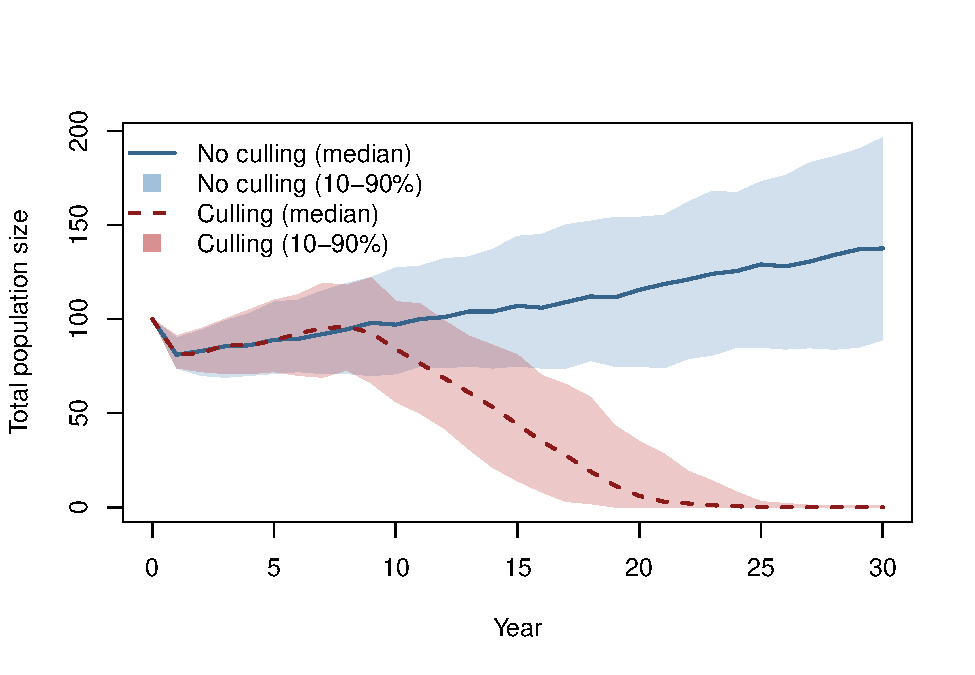
\includegraphics[keepaspectratio]{BB512_files/BB512_files/figure-latex/mpm_sim_reps_cull-1.pdf}}

\section{Student exercises (for a class handout)}\label{student-exercises-for-a-class-handout}

\subsection{Exercise: Projection interval sanity check}\label{exercise-projection-interval-sanity-check}

\begin{enumerate}
\def\labelenumi{\arabic{enumi}.}
\tightlist
\item
  In the tutorial, \textbackslash(\textbackslash Delta t = 1\textbackslash) year. Write one sentence explaining what that means.
\item
  Suppose you wanted \textbackslash(\textbackslash Delta t = 1\textbackslash) month. What changes would you need to make to the interpretation of:

  \begin{itemize}
  \tightlist
  \item
    \textbackslash(P\_A\textbackslash)?
  \item
    \textbackslash(F\_A\textbackslash)?
  \end{itemize}
\item
  Name one real reason you might prefer monthly time steps over yearly ones.
\end{enumerate}

\subsection{Exercise: Change one vital rate and re-run projections}\label{exercise-change-one-vital-rate-and-re-run-projections}

\begin{enumerate}
\def\labelenumi{\arabic{enumi}.}
\tightlist
\item
  Reduce adult survival from \textbackslash(P\_A = 0.80\textbackslash) to \textbackslash(P\_A = 0.70\textbackslash). Recompute:

  \begin{itemize}
  \tightlist
  \item
    the deterministic projection plot,
  \item
    \textbackslash(\textbackslash lambda\textbackslash).
  \end{itemize}
\item
  Does the population grow or decline now? How can you tell?
\end{enumerate}

\subsection{Exercise: Culling as management}\label{exercise-culling-as-management}

\begin{enumerate}
\def\labelenumi{\arabic{enumi}.}
\tightlist
\item
  In the simulation, cull 5 adults per year from year 10. Increase this to 10 adults per year.
\item
  Compare the median population trajectory and the uncertainty bands.
\item
  To identify which stage is most impactful, run the same culling intensity for each stage separately (juveniles, subadults, adults), then compare results. Which stage has the largest effect, and why?
\end{enumerate}

\subsection{Exercise: Contraception treatment (reduced fecundity)}\label{exercise-contraception-treatment-reduced-fecundity}

Design a second management treatment where fecundity is reduced instead of removing individuals.

\begin{enumerate}
\def\labelenumi{\arabic{enumi}.}
\tightlist
\item
  Keep survival/transition rates unchanged, but reduce fecundity after year 10 with a 90\% effective contraceptive treatment (for example, multiply \texttt{F\_A} by 0.1 from year 10 onward).
\item
  Implement this as a time-dependent fecundity value inside the yearly loop (for example, \texttt{F\_A\_t}), and use \texttt{F\_A\_t} in the births step.
\item
  Run replicate simulations for:

  \begin{itemize}
  \tightlist
  \item
    baseline (no treatment),
  \item
    culling treatment,
  \item
    contraception treatment.
  \end{itemize}
\item
  Compare all three scenarios in one figure and discuss which treatment gives the largest reduction in population growth.
\end{enumerate}

\section{Notes and extensions}\label{notes-and-extensions}

\begin{itemize}
\tightlist
\item
  If you include juvenile stasis (juveniles surviving but remaining juveniles), add a \textbackslash(P\_J\textbackslash) term and include it in the matrix and simulation.
\item
  The deterministic matrix model is most useful for \emph{structure} and \emph{long-term behaviour} (\textbackslash(\textbackslash lambda\textbackslash), stable stage structure, elasticities).
\item
  Stochastic simulations are most useful for \emph{short-term variability} and \emph{scenario exploration} (management, uncertainty, risk).
\end{itemize}

\chapter*{Part 3: Population Genetics and Evolution}\label{part-3}
\addcontentsline{toc}{chapter}{Part 3: Population Genetics and Evolution}

This part introduces the genetic mechanisms that shape evolutionary change. You will connect allele frequencies to forces like selection, drift, and heritability.

By the end of Part 3, you should be able to:

\begin{itemize}
\tightlist
\item
  Use Hardy-Weinberg logic to interpret allele and genotype frequencies.
\item
  Simulate allele frequency change under different evolutionary forces.
\item
  Estimate heritability and interpret its evolutionary implications.
\end{itemize}

\chapter{Hardy-Weinberg equilibrium}\label{hardy-weinberg-equilibrium}

Learning outcomes. By the end of this practical you should be able to:

\begin{itemize}
\tightlist
\item
  Explain the difference between alleles and genotypes.
\item
  Calculate expected genotype frequencies from allele frequencies, and allele frequencies from the frequency of a recessive genotype.
\item
  Estimate allele frequencies from observed genotype counts and compare the observed counts with those expected under Hardy-Weinberg equilibrium (HWE).
\item
  List the assumptions of HWE and explain what a departure from HWE might, and might not, tell you.
\end{itemize}

\section{Background}\label{background-12}

Hardy-Weinberg equilibrium is a fundamental concept in population genetics for understanding the genetic dynamics of populations. Named after British mathematician G.H. Hardy and German physician Wilhelm Weinberg, this principle describes the stable genetic proportions in a population under specific conditions of no evolution.

In an idealised population, where mating is random, genetic mutations are absent, natural selection is not acting, and there is no gene flow or genetic drift, the frequencies of alleles and genotypes remain constant across generations.

The Hardy-Weinberg equilibrium provides a baseline against which real populations can be compared, allowing researchers to detect factors that may cause deviations from this equilibrium and, in turn, understand the forces driving evolution and genetic changes within populations.

In this practical we will learn more about HWE and practise solving some HWE-related problems.

The key formulae of the Hardy-Weinberg Equilibrium are:

Equation 1: \(p + q = 1\)

and

Equation 2: \(p^2 + 2pq + q^2 = 1\).

Let's first consider where these equations come from. First, Equation 1.

In a diploid organism, each individual carries two alleles for a particular gene. Let's consider a gene with two alleles, A and a. In a given population:

{\def\LTcaptype{none} % do not increment counter
\begin{longtable}[]{@{}ll@{}}
\toprule\noalign{}
Symbol & Meaning \\
\midrule\noalign{}
\endhead
\bottomrule\noalign{}
\endlastfoot
\(p\) & Frequency of allele A \\
\(q\) & Frequency of allele a \\
\end{longtable}
}

The sum of the frequencies of these two alleles in the population must equal 1, as they are the only two possibilities for this gene, so \(p+q=1\).

Note that dominance affects the \emph{phenotype}, not the allele frequency. A dominant allele can be rare and a recessive allele can be common.

When genotype counts are available, we can calculate allele frequencies directly by counting allele copies:

\[
p = \frac{2n_{AA} + n_{Aa}}{2N}, \qquad
q = \frac{2n_{aa} + n_{Aa}}{2N}.
\]

Here, \(n_{AA}\), \(n_{Aa}\) and \(n_{aa}\) are the numbers of individuals with each genotype, and \(N = n_{AA} + n_{Aa} + n_{aa}\). Each homozygote contributes two copies of the same allele, while each heterozygote contributes one copy of each allele. These calculations do not require HWE. Once we know \(p\) and \(q\), we can calculate the expected genotype counts under HWE as \(Np^2\), \(N(2pq)\) and \(Nq^2\), and compare them with the observed counts.

Equation 1 serves as the foundational stepping stone for Equation 2. In Equation 1, we establish the sum of allele frequencies, \(p\) and \(q\), in the gene pool. This equation sets the stage for the more complex Equation 2, where we translate these allele frequencies into genotype frequencies for the population.

We can derive Equation 2 based on the gene pool and random mating. Let's consider a mating event between two random alleles. The possible combinations of alleles are:

\begin{itemize}
\tightlist
\item
  \(p \times p = p^2\) (AA)
\item
  \(q \times q = q^2\) (aa)
\item
  \(p \times q = pq\) (Aa)
\item
  \(q \times p = pq\) (aA)
\end{itemize}

Notice that we have two \(pq\) terms (Aa and aA). The order of alleles doesn't matter, so they are summed together: \(2pq\).

So, the total probability for all possible combinations is:

\(p^2 + 2pq + q^2\).

This must equal 1 (100\% probability), which gives us Equation 2:

\(p^2 + 2pq + q^2 = 1\).

In these formulae, \(p^2\) is the frequency of the homozygous AA genotype, \(q^2\) is the frequency of the homozygous aa genotype and \(2pq\) is the frequency of the heterozygous Aa genotype. From these equations we can produce the following plot, which shows the expected genotype frequencies at HWE for any allele frequency. HWE can occur at any allele frequency, but once the allele frequency is known, the expected genotype frequencies are fixed by Equation 2. (It is a common misconception that the three genotypes should occur in a 1:2:1 ratio, or that allele frequencies should tend towards 50\% \(p\) and 50\% \(q\).)

Given a small amount of information it is possible to figure out what the allele and genotype frequencies should be \emph{if the population is at HWE}.

If a population is NOT at HWE, that is a signal worth investigating. It may mean that one of the assumptions below is violated, but apparent departures can also arise from genotyping errors or simple chance in a small sample.

\begin{figure}
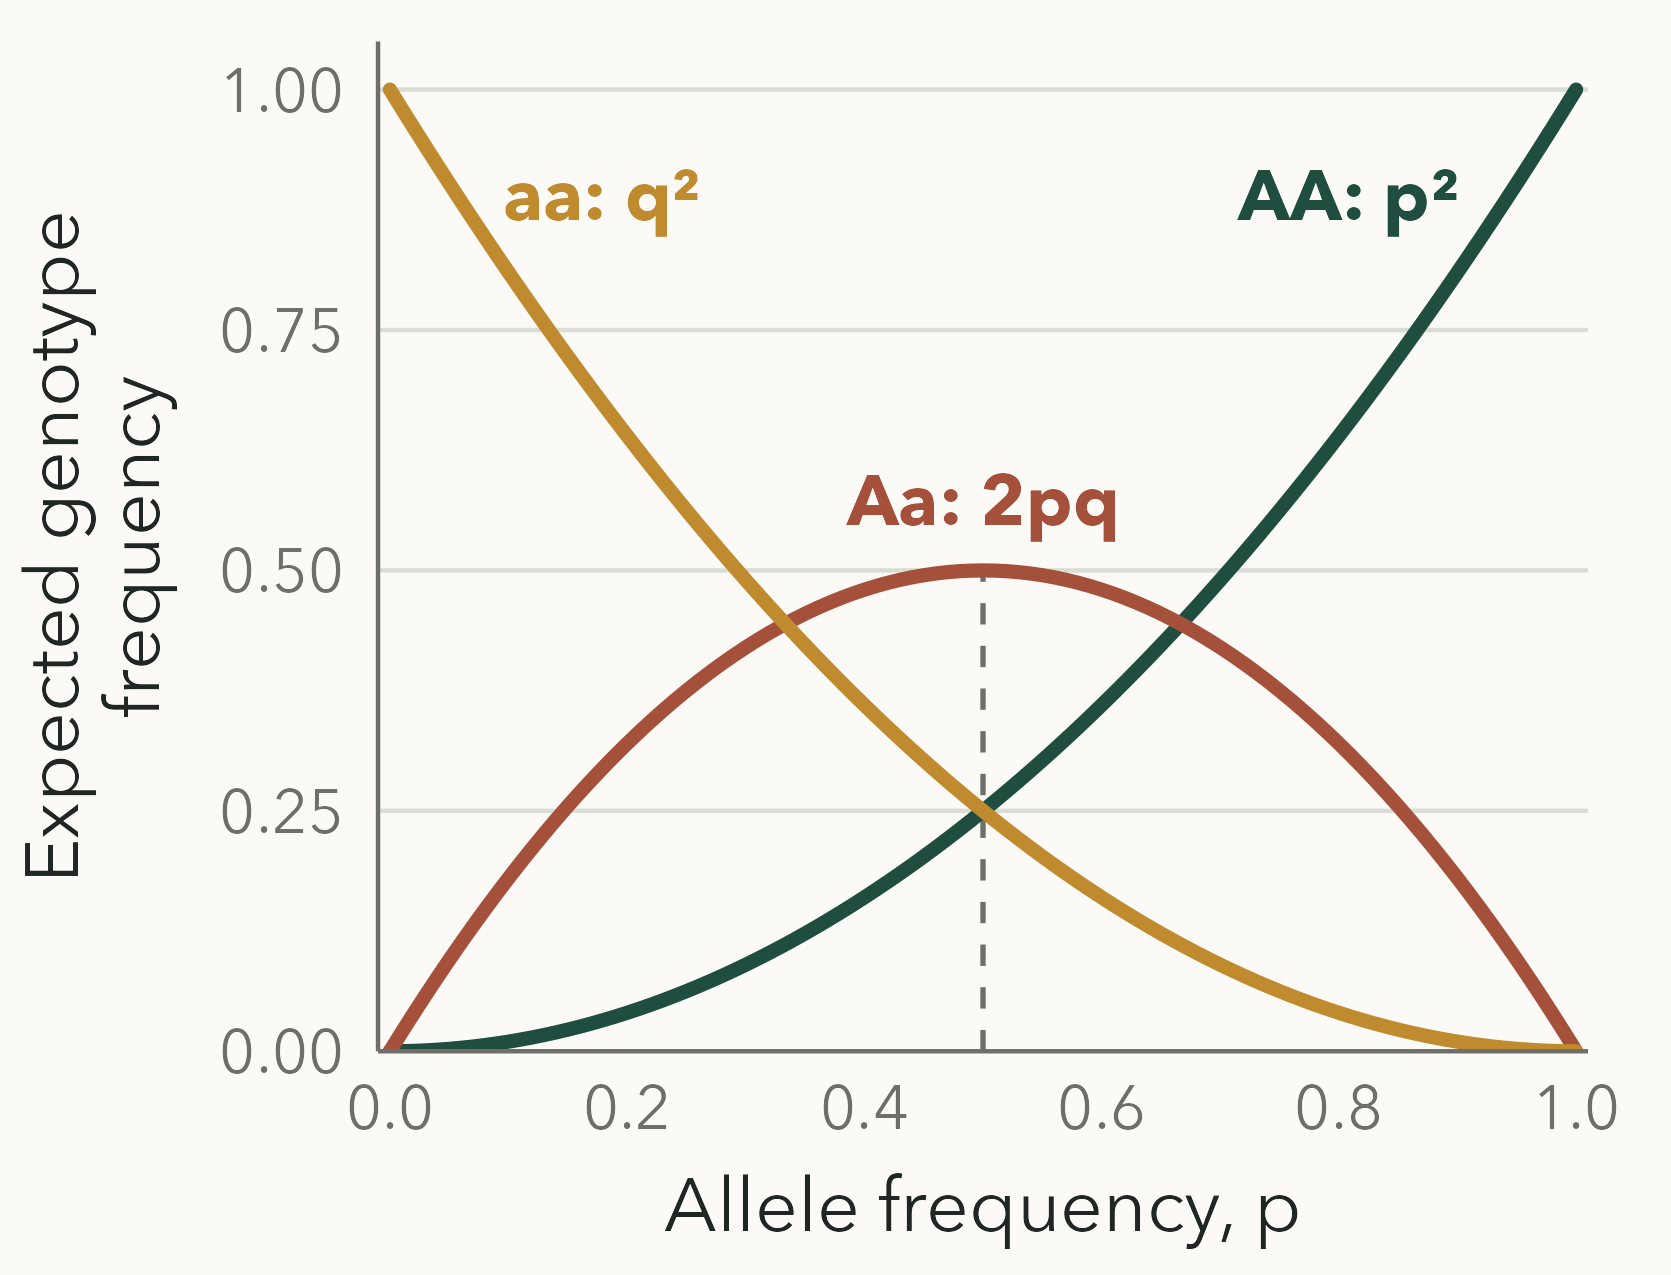
\includegraphics[width=0.7\linewidth]{lecture_figures/hardy_weinberg/output/half/14_genotype_frequencies} \caption{The Hardy-Weinberg Equilibrium. The lines show the expected genotype frequencies at HWE for each allele frequency, p.}\label{fig:hardyweinberg}
\end{figure}

\section{Assumptions of Hardy-Weinberg Equilibrium}\label{assumptions-of-hardy-weinberg-equilibrium}

For a population to be in Hardy-Weinberg Equilibrium, certain assumptions must be met:

\begin{itemize}
\tightlist
\item
  Random mating: There is no preference in mate selection based on genotype.
\item
  No mutation: Alleles do not change into other alleles, so mutation does not alter allele frequencies.
\item
  Very large population size: Random sampling has a negligible effect on allele frequencies (genetic drift).
\item
  No gene flow: Migration does not transfer alleles into or out of the population's breeding gene pool.
\item
  No natural selection: All genotypes in the population have an equal chance of reproductive success.
\end{itemize}

These assumptions do two different jobs. Random mating is what produces the Hardy-Weinberg genotype proportions (\(p^2 : 2pq : q^2\)) in each generation. The other four (no mutation, no drift, no gene flow and no selection) are what keep the allele frequencies themselves constant from one generation to the next.

Any deviation from these assumptions could result in a population that is not in Hardy-Weinberg Equilibrium.

\section{Worked example}\label{worked-example-7}

Unless a problem states otherwise, assume that the population is at HWE. This matters: working back from the frequency of a recessive genotype to an allele frequency (as below) is only valid if the population is at HWE.

Suppose 16\% of individuals have the recessive genotype, aa, so \(q^2 = 0.16\). What proportion of the population would we expect to be heterozygous?

\begin{enumerate}
\def\labelenumi{\arabic{enumi}.}
\tightlist
\item
  Calculate \(q = \sqrt{0.16} = 0.4\).
\item
  Calculate \(p = 1 - q = 0.6\).
\item
  Calculate the heterozygote frequency: \(2pq = 2(0.6)(0.4) = 0.48\).
\end{enumerate}

We therefore expect 48\% of individuals to be heterozygous (Aa), assuming the population is at HWE.

\section{Your task}\label{your-task-13}

Tackle the following problems, using the HWE theory outlined above. Worked solutions are given in Section \ref{solutions-hardy-weinberg-equilibrium}.

\subsection{Problem \#1.}\label{problem-1.}

A population has two alleles, A and a, at a gene of interest. The frequency of allele A is 0.7. Assuming the population is at HWE, calculate the following:

\begin{itemize}
\tightlist
\item
  The frequency of allele a.
\item
  The expected frequencies of the genotypes AA, Aa and aa.
\item
  The frequencies of the two possible phenotypes if A is completely dominant over a.
\end{itemize}

\subsection{Problem \#2.}\label{problem-2.}

Sickle-cell disease is caused by variants of the haemoglobin gene. In this simplified two-allele example, people with two copies of the usual allele (HbA/HbA) do not have sickle-cell disease, but lack the protection against severe malaria associated with sickle-cell trait. People with two copies of the sickle-cell allele (HbS/HbS) have sickle-cell disease: their red blood cells can become rigid and sickle-shaped, causing serious illness. Heterozygous people (HbA/HbS) have sickle-cell \emph{trait}. Most have no symptoms of sickle-cell disease, and they have increased protection against severe malaria. In regions where malaria is common, this can give heterozygotes a survival advantage over either homozygote.

\begin{itemize}
\tightlist
\item
  In a population from a malaria-endemic region, 9\% of babies are born with sickle-cell disease (HbS/HbS). Assuming the population is at HWE at birth, what percentage of babies will be heterozygous (HbA/HbS), and so more resistant to severe malaria?
\end{itemize}

Because of the survival differences described above, genotype frequencies among \emph{adults} in such a population are not expected to stay at HWE. This is why the question asks about babies at birth.

\subsection{Problem \#3.}\label{problem-3.}

You genotype a sample of 200 individuals from a population at a gene with two alleles, A and a. You find 120 AA, 40 Aa and 40 aa individuals. This time, do not assume the population is at HWE: assess whether the observed counts match HWE expectations. A descriptive comparison is sufficient for this exercise; you do not need to perform a formal statistical test.

\begin{itemize}
\tightlist
\item
  Calculate the frequencies of alleles A and a from the genotype counts. (Hint: 200 diploid individuals carry 400 allele copies, and each heterozygote carries one copy of each allele.)
\item
  Calculate the expected number of each genotype if the population were at HWE.
\item
  Compare the observed and expected counts. Is there an excess or a deficit of heterozygotes? Suggest some reasons why a population might show this pattern.
\end{itemize}

\subsection{Problem \#4.}\label{problem-4.}

Within a population of butterflies, brown (B) is completely dominant over white (b), and 40\% of all butterflies are white. Assuming the population is at HWE, calculate the following:

\begin{itemize}
\tightlist
\item
  The percentage of butterflies in the population that are heterozygous.
\item
  The frequency of homozygous dominant individuals.
\item
  \emph{Extension:} Of the brown butterflies, what proportion would you expect to be heterozygous? (Think carefully about what the denominator should be.)
\end{itemize}

\section{Takeaways}\label{takeaways-13}

\begin{itemize}
\tightlist
\item
  Hardy-Weinberg equilibrium provides a baseline for detecting evolutionary forces.
\item
  Allele frequencies (\(p\), \(q\)) determine genotype frequencies (\(p^2\), \(2pq\), \(q^2\)).
\item
  Comparing observed genotype counts with HWE expectations can reveal a departure from HWE. A departure identifies a pattern worth investigating (for example, a violated assumption, genotyping error or chance in a small sample), not its cause.
\end{itemize}

\chapter{The Gene Pool Model}\label{the-gene-pool-model}

\section{Background}\label{background-13}

A central goal in evolutionary biology is to understand variation -- including genetic variation -- and how it changes through time. One important idea is the ``gene pool,'' which contains all the different versions of genes (alleles) within a group of organisms. These alleles influence phenotypic traits and other characteristics. To grasp how populations evolve, we need to understand how allele frequencies change in a population. Over time, genetic diversity changes as the relative numbers of alleles change. Some alleles may be lost from the population while others may become ``fixed'' -- where the allele is the only one left, so every individual in the population carries it.

When no other process is acting, allele frequencies still change by chance. This is \textbf{genetic drift}. The main factor that determines the strength of drift is population size. In small populations, ``sampling error'' means that, just by chance, large changes often occur in allele frequencies. In large populations, dramatic changes are much less likely.

Two related concepts are critical in understanding genetic drift: bottlenecks and founder effects. A \textbf{genetic bottleneck} occurs when a population is dramatically reduced in size, for example by an environmental catastrophe. During a bottleneck, allele frequencies (and genetic diversity) can change dramatically because of sampling effects. A \textbf{founder effect} is a similar scenario, where a small group (a sample from the population) establishes a new population. Because the new population starts from a small sample of the ancestral population, it can have a rather different genetic composition from the ancestral population.

Learning outcomes:

\begin{itemize}
\tightlist
\item
  Greater understanding of evolution via genetic drift (neutral evolution).
\item
  Understanding of genetic bottlenecks and founder effects.
\item
  Understanding the relationship between stochasticity and genetic variation.
\item
  Use of R for exploring biological phenomena.
\end{itemize}

\section{Your task}\label{your-task-14}

In this practical, you will use R to simulate how allele frequencies change in a population over generations. By changing population size, starting frequency and the history of the population, you will see how drift behaves in different situations.

The practical has four parts:

\begin{enumerate}
\def\labelenumi{\arabic{enumi}.}
\tightlist
\item
  \textbf{The gene pool.} Build a gene pool and see that the gene pool in the next generation is a \emph{sample} of the current one.
\item
  \textbf{Drift through time.} Project allele frequency through time and investigate the importance of population size.
\item
  \textbf{Many populations.} Repeat the simulation many times to estimate the probability that an allele is fixed or lost, including for a rare (new) allele.
\item
  \textbf{Bottlenecks and founder effects.} Modify the code to simulate a population that passes through a period of small size, and a new population founded by a few individuals.
\end{enumerate}

\textbf{Before you start, make a prediction.} Imagine two populations, each starting with allele \emph{A} at a frequency of 0.5. One has 20 individuals and the other has 1000. Sketch what you expect the frequency of \emph{A} to look like over 100 generations in each population. Which population do you expect to lose one of its alleles first? Keep your sketch, and compare it with your simulations in Part 2.

\subsection{The model and its assumptions}\label{the-model-and-its-assumptions}

Our model is a simple version of the \textbf{Wright-Fisher model} of population genetics. It assumes:

\begin{itemize}
\tightlist
\item
  a single locus with two alleles, \emph{A} and \emph{a};
\item
  a constant number of diploid individuals, N, so the gene pool contains 2N alleles;
\item
  non-overlapping generations: all adults are replaced by their offspring each generation;
\item
  random mating, so each new allele is a random draw from the parents' gene pool;
\item
  no selection, no mutation and no migration.
\end{itemize}

So the \emph{only} thing that changes allele frequencies is chance. Keep these assumptions in mind: we come back to them at the end.

\section{Part 1: A simple model}\label{part-1-a-simple-model}

We will first aim to get an understanding of what a gene pool is, using a simple model. We will use R to make a gene pool, then look at how allele frequency in the gene pool changes over a single generation.

\subsection{The gene pool}\label{the-gene-pool}

To establish the gene pool we first set the population size. I set this to be reasonably large, at 500 individuals.

\begin{Shaded}
\begin{Highlighting}[]
\NormalTok{pop\_size }\OtherTok{\textless{}{-}} \DecValTok{500}
\end{Highlighting}
\end{Shaded}

There are two alleles (gene variants) per individual: one allele came from the father, and one from the mother.

Therefore, the gene pool contains 2 x N alleles (in this case, 1000 alleles).

\begin{Shaded}
\begin{Highlighting}[]
\NormalTok{pool\_size }\OtherTok{\textless{}{-}}\NormalTok{ pop\_size }\SpecialCharTok{*} \DecValTok{2}
\end{Highlighting}
\end{Shaded}

I now set the initial allele frequency to be 0.5. You can use other values, but 0.5 is best to start with.

\begin{Shaded}
\begin{Highlighting}[]
\NormalTok{initial\_frequency\_A }\OtherTok{\textless{}{-}} \FloatTok{0.5}
\NormalTok{initial\_frequency\_a }\OtherTok{\textless{}{-}} \DecValTok{1} \SpecialCharTok{{-}}\NormalTok{ initial\_frequency\_A}
\end{Highlighting}
\end{Shaded}

We can now calculate the \textbf{number} of \emph{A} and \emph{a} alleles, by multiplying the frequency by the pool size and rounding the result to the closest whole number.

\begin{Shaded}
\begin{Highlighting}[]
\NormalTok{number\_A }\OtherTok{\textless{}{-}} \FunctionTok{round}\NormalTok{(initial\_frequency\_A }\SpecialCharTok{*}\NormalTok{ pool\_size)}
\NormalTok{number\_a }\OtherTok{\textless{}{-}} \FunctionTok{round}\NormalTok{(initial\_frequency\_a }\SpecialCharTok{*}\NormalTok{ pool\_size)}
\end{Highlighting}
\end{Shaded}

Following this, the gene pool can be filled like this.
What we are saying here is ``repeat \texttt{A}, \texttt{number\_A} times, then repeat \texttt{a} \texttt{number\_a} times''.

\begin{Shaded}
\begin{Highlighting}[]
\NormalTok{gene\_pool }\OtherTok{\textless{}{-}} \FunctionTok{c}\NormalTok{(}\FunctionTok{rep}\NormalTok{(}\StringTok{"A"}\NormalTok{, number\_A), }\FunctionTok{rep}\NormalTok{(}\StringTok{"a"}\NormalTok{, number\_a))}
\end{Highlighting}
\end{Shaded}

Output (counts in the initial gene pool):

\begin{verbatim}
## gene_pool
##   a   A 
## 500 500
\end{verbatim}

We can express these numbers as allele frequencies (i.e.~as proportions of the total) by wrapping the \texttt{table} command with \texttt{prop.table} like this:

\begin{Shaded}
\begin{Highlighting}[]
\FunctionTok{prop.table}\NormalTok{(}\FunctionTok{table}\NormalTok{(gene\_pool))}
\end{Highlighting}
\end{Shaded}

\begin{verbatim}
## gene_pool
##   a   A 
## 0.5 0.5
\end{verbatim}

\subsection{Projecting allele frequency over one time step}\label{projecting-allele-frequency-over-one-time-step}

Let's assume the population size remains constant at N = 500.

During the next time step (i.e.~1 generation), the individuals in the population mate with each other randomly. We can use the \texttt{sample} function to simulate this.

This code is saying ``\textbf{sample, from the gene pool, 1000 alleles, with replacement}''. We need to sample \(2 \times\) the population size because each individual contains two alleles. We sample \emph{with replacement} because any allele in the parents' gene pool can be passed on to more than one offspring (or to none).

\begin{Shaded}
\begin{Highlighting}[]
\NormalTok{new\_gene\_pool }\OtherTok{\textless{}{-}} \FunctionTok{sample}\NormalTok{(gene\_pool, }\DecValTok{2} \SpecialCharTok{*}\NormalTok{ pop\_size, }\AttributeTok{replace =} \ConstantTok{TRUE}\NormalTok{)}
\end{Highlighting}
\end{Shaded}

Let's look at the allele frequency in the new gene pool. It should be similar, but probably not exactly the same as the initial gene pool.

\begin{Shaded}
\begin{Highlighting}[]
\FunctionTok{prop.table}\NormalTok{(}\FunctionTok{table}\NormalTok{(new\_gene\_pool))}
\end{Highlighting}
\end{Shaded}

\begin{verbatim}
## new_gene_pool
##     a     A 
## 0.491 0.509
\end{verbatim}

There are still 500 individuals, but the allele frequencies are (probably) not exactly the same as in the initial gene pool. The reason is that the new gene pool is a random sample, not simply a carbon copy.

\textbf{Try to vary the population size and do this several times at small and large population sizes.} You should notice that the frequencies are more similar to the starting frequency, and to each other, when you repeat this for large population sizes than for small population sizes.

\section{Part 2: Simulation of allele frequency through time}\label{part-2-simulation-of-allele-frequency-through-time}

To simulate the passage of time, we need to do this sampling procedure many times.

We can do this using a loop in R. In our loop, we repeat the gene pool sampling process once per generation. Each time we go through the loop, we sample alleles from the \emph{old} gene pool at time \(t\) to create a \emph{new} gene pool for time \(t+1\). Each time through the loop we also calculate the allele frequency of \emph{A}, so we can track how it changes through time.

Let's set up a simulation that runs for 100 generations, starting with a small population of 20 individuals.
You can copy and paste this code, which is a complete gene pool model.

\begin{Shaded}
\begin{Highlighting}[]
\CommentTok{\# Set the population size and number of generations}
\NormalTok{pop\_size }\OtherTok{\textless{}{-}} \DecValTok{20}
\NormalTok{n\_gen }\OtherTok{\textless{}{-}} \DecValTok{100}

\CommentTok{\# Set up an empty vector of length n\_gen to contain results}
\NormalTok{allele\_freq\_A }\OtherTok{\textless{}{-}} \FunctionTok{rep}\NormalTok{(}\ConstantTok{NA}\NormalTok{, n\_gen)}

\CommentTok{\# Put in an initial value for frequency of A}
\NormalTok{allele\_freq\_A[}\DecValTok{1}\NormalTok{] }\OtherTok{\textless{}{-}} \FloatTok{0.5}

\CommentTok{\# Establish the initial gene pool and name it gene\_pool\_time\_n}
\CommentTok{\# This part looks complicated, but it just condenses the code}
\CommentTok{\# from Part 1 into one line.}
\NormalTok{gene\_pool\_time\_n }\OtherTok{\textless{}{-}} \FunctionTok{c}\NormalTok{(}
  \FunctionTok{rep}\NormalTok{(}\StringTok{"A"}\NormalTok{, }\FunctionTok{round}\NormalTok{(}\DecValTok{2} \SpecialCharTok{*}\NormalTok{ allele\_freq\_A[}\DecValTok{1}\NormalTok{] }\SpecialCharTok{*}\NormalTok{ pop\_size)),}
  \FunctionTok{rep}\NormalTok{(}\StringTok{"a"}\NormalTok{, }\FunctionTok{round}\NormalTok{(}\DecValTok{2} \SpecialCharTok{*}\NormalTok{ (}\DecValTok{1} \SpecialCharTok{{-}}\NormalTok{ allele\_freq\_A[}\DecValTok{1}\NormalTok{]) }\SpecialCharTok{*}\NormalTok{ pop\_size))}
\NormalTok{)}

\ControlFlowTok{for}\NormalTok{ (i }\ControlFlowTok{in} \DecValTok{2}\SpecialCharTok{:}\NormalTok{n\_gen) \{}
  \CommentTok{\# Sample 2N alleles, with replacement, to make the next generation}
\NormalTok{  gene\_pool\_time\_n\_plus\_1 }\OtherTok{\textless{}{-}} \FunctionTok{sample}\NormalTok{(gene\_pool\_time\_n,}
\NormalTok{    pop\_size }\SpecialCharTok{*} \DecValTok{2}\NormalTok{,}
    \AttributeTok{replace =} \ConstantTok{TRUE}
\NormalTok{  )}
  \CommentTok{\# Calculate the frequency of A in the new gene pool}
\NormalTok{  gene\_pool\_table }\OtherTok{\textless{}{-}} \FunctionTok{table}\NormalTok{(}\FunctionTok{factor}\NormalTok{(gene\_pool\_time\_n\_plus\_1,}
                                  \AttributeTok{levels =} \FunctionTok{c}\NormalTok{(}\StringTok{"A"}\NormalTok{, }\StringTok{"a"}\NormalTok{)))}
\NormalTok{  allele\_freq\_A[i] }\OtherTok{\textless{}{-}}\NormalTok{ gene\_pool\_table[}\StringTok{"A"}\NormalTok{] }\SpecialCharTok{/} \FunctionTok{sum}\NormalTok{(gene\_pool\_table)}

  \CommentTok{\# Replace the old gene pool with the new one.}
\NormalTok{  gene\_pool\_time\_n }\OtherTok{\textless{}{-}}\NormalTok{ gene\_pool\_time\_n\_plus\_1}
\NormalTok{\}}
\end{Highlighting}
\end{Shaded}

Now we can plot this result (Figure \ref{fig:simulationplot}).

\begin{Shaded}
\begin{Highlighting}[]
\FunctionTok{plot}\NormalTok{(}\DecValTok{1}\SpecialCharTok{:}\NormalTok{n\_gen, allele\_freq\_A, }\AttributeTok{type =} \StringTok{"l"}\NormalTok{,}
     \AttributeTok{xlab =} \StringTok{"Generation"}\NormalTok{,}
     \AttributeTok{ylab =} \StringTok{"Frequency of allele A"}\NormalTok{,}
     \AttributeTok{ylim =} \FunctionTok{c}\NormalTok{(}\DecValTok{0}\NormalTok{, }\DecValTok{1}\NormalTok{))}
\end{Highlighting}
\end{Shaded}

\begin{figure}
\centering
\pandocbounded{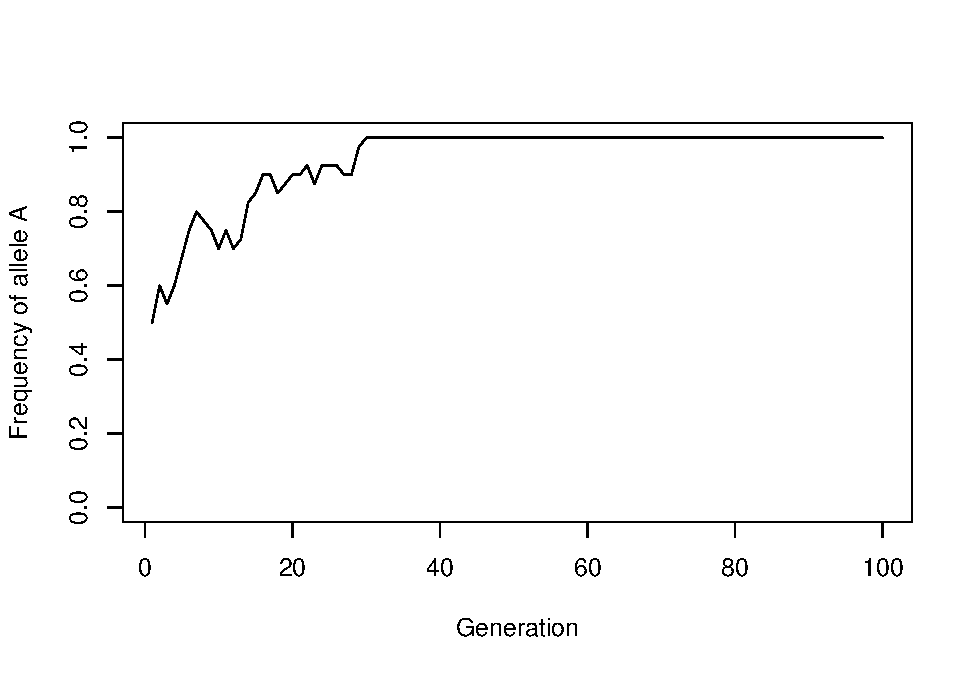
\includegraphics[keepaspectratio,alt={\label{fig:simulationplot}Simulation of allele frequency through time in a population of 20 individuals}]{BB512_files/BB512_files/figure-latex/simulationplot-1.pdf}}
\caption{\label{fig:simulationplot}Simulation of allele frequency through time in a population of 20 individuals}
\end{figure}

Tip: make a new script and paste the code loop along with the plot command so that you can run both together easily.

Run the code several times with \texttt{pop\_size\ \textless{}-\ 20}, then several times with \texttt{pop\_size\ \textless{}-\ 1000}. Compare the results with the prediction you made at the start.

\begin{itemize}
\tightlist
\item
  How does population size affect the variation through time in allele frequencies? Why do you see these patterns?
\item
  With 20 individuals, does \emph{A} always end up fixed (frequency 1), or is it sometimes lost (frequency 0)?
\item
  When the population size is large (say 1000), can you see an allele become fixed within 100 generations? Do you think it could happen if you ran the simulation for much longer? (Try \texttt{n\_gen\ \textless{}-\ 3000}. It may take a little while to run.)
\end{itemize}

\section{Part 3: Many populations}\label{part-3-many-populations}

A single run of the simulation is like watching a single population. To answer questions about \emph{probability} (for example, ``how likely is it that \emph{A} is fixed?'') we need to watch many populations: we run the same simulation many times and count the outcomes.

To make this easy, we first wrap the loop from Part 2 into a \textbf{function}. A function is a reusable piece of code: you give it some inputs (here, population size, number of generations and the starting frequency of \emph{A}), and it returns the frequency of \emph{A} in every generation.

\begin{Shaded}
\begin{Highlighting}[]
\NormalTok{simulate\_gene\_pool }\OtherTok{\textless{}{-}} \ControlFlowTok{function}\NormalTok{(pop\_size, n\_gen, initial\_freq\_A) \{}
\NormalTok{  allele\_freq\_A }\OtherTok{\textless{}{-}} \FunctionTok{rep}\NormalTok{(}\ConstantTok{NA}\NormalTok{, n\_gen)}
\NormalTok{  allele\_freq\_A[}\DecValTok{1}\NormalTok{] }\OtherTok{\textless{}{-}}\NormalTok{ initial\_freq\_A}

\NormalTok{  gene\_pool\_time\_n }\OtherTok{\textless{}{-}} \FunctionTok{c}\NormalTok{(}
    \FunctionTok{rep}\NormalTok{(}\StringTok{"A"}\NormalTok{, }\FunctionTok{round}\NormalTok{(}\DecValTok{2} \SpecialCharTok{*}\NormalTok{ initial\_freq\_A }\SpecialCharTok{*}\NormalTok{ pop\_size)),}
    \FunctionTok{rep}\NormalTok{(}\StringTok{"a"}\NormalTok{, }\FunctionTok{round}\NormalTok{(}\DecValTok{2} \SpecialCharTok{*}\NormalTok{ (}\DecValTok{1} \SpecialCharTok{{-}}\NormalTok{ initial\_freq\_A) }\SpecialCharTok{*}\NormalTok{ pop\_size))}
\NormalTok{  )}

  \ControlFlowTok{for}\NormalTok{ (i }\ControlFlowTok{in} \DecValTok{2}\SpecialCharTok{:}\NormalTok{n\_gen) \{}
\NormalTok{    gene\_pool\_time\_n\_plus\_1 }\OtherTok{\textless{}{-}} \FunctionTok{sample}\NormalTok{(gene\_pool\_time\_n,}
\NormalTok{      pop\_size }\SpecialCharTok{*} \DecValTok{2}\NormalTok{,}
      \AttributeTok{replace =} \ConstantTok{TRUE}
\NormalTok{    )}
\NormalTok{    gene\_pool\_table }\OtherTok{\textless{}{-}} \FunctionTok{table}\NormalTok{(}\FunctionTok{factor}\NormalTok{(gene\_pool\_time\_n\_plus\_1,}
                                    \AttributeTok{levels =} \FunctionTok{c}\NormalTok{(}\StringTok{"A"}\NormalTok{, }\StringTok{"a"}\NormalTok{)))}
\NormalTok{    allele\_freq\_A[i] }\OtherTok{\textless{}{-}}\NormalTok{ gene\_pool\_table[}\StringTok{"A"}\NormalTok{] }\SpecialCharTok{/} \FunctionTok{sum}\NormalTok{(gene\_pool\_table)}
\NormalTok{    gene\_pool\_time\_n }\OtherTok{\textless{}{-}}\NormalTok{ gene\_pool\_time\_n\_plus\_1}
\NormalTok{  \}}
  \FunctionTok{return}\NormalTok{(allele\_freq\_A)}
\NormalTok{\}}
\end{Highlighting}
\end{Shaded}

Now we can use \texttt{replicate} to run the function many times. Here we simulate 20 populations, each of 20 individuals, for 100 generations. The result is a matrix with one row per generation and one column per population. The \texttt{matplot} function plots each column as a separate line (Figure \ref{fig:replicateplot}).

\begin{Shaded}
\begin{Highlighting}[]
\NormalTok{n\_gen }\OtherTok{\textless{}{-}} \DecValTok{100}
\NormalTok{results }\OtherTok{\textless{}{-}} \FunctionTok{replicate}\NormalTok{(}\DecValTok{20}\NormalTok{, }\FunctionTok{simulate\_gene\_pool}\NormalTok{(}\AttributeTok{pop\_size =} \DecValTok{20}\NormalTok{, }\AttributeTok{n\_gen =}\NormalTok{ n\_gen,}
                                            \AttributeTok{initial\_freq\_A =} \FloatTok{0.5}\NormalTok{))}

\FunctionTok{matplot}\NormalTok{(}\DecValTok{1}\SpecialCharTok{:}\NormalTok{n\_gen, results, }\AttributeTok{type =} \StringTok{"l"}\NormalTok{, }\AttributeTok{lty =} \DecValTok{1}\NormalTok{,}
        \AttributeTok{xlab =} \StringTok{"Generation"}\NormalTok{,}
        \AttributeTok{ylab =} \StringTok{"Frequency of allele A"}\NormalTok{,}
        \AttributeTok{ylim =} \FunctionTok{c}\NormalTok{(}\DecValTok{0}\NormalTok{, }\DecValTok{1}\NormalTok{))}
\end{Highlighting}
\end{Shaded}

\begin{figure}
\centering
\pandocbounded{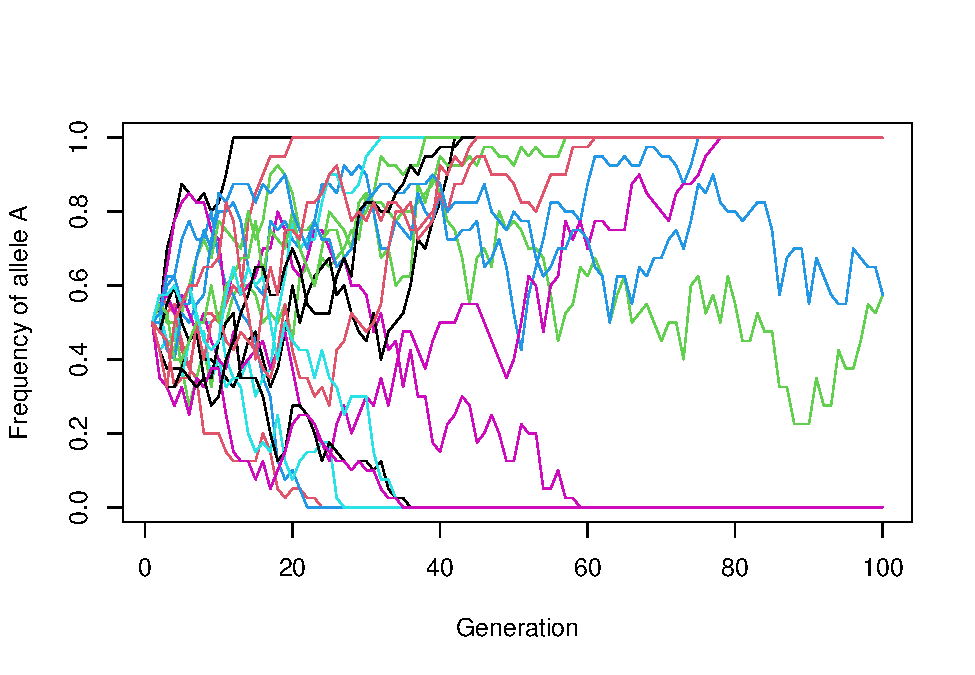
\includegraphics[keepaspectratio,alt={\label{fig:replicateplot}Twenty replicate populations of 20 individuals, each starting with allele A at a frequency of 0.5}]{BB512_files/BB512_files/figure-latex/replicateplot-1.pdf}}
\caption{\label{fig:replicateplot}Twenty replicate populations of 20 individuals, each starting with allele A at a frequency of 0.5}
\end{figure}

We can count the outcomes by looking at the last row of the matrix (the final generation):

\begin{Shaded}
\begin{Highlighting}[]
\NormalTok{final\_freq }\OtherTok{\textless{}{-}}\NormalTok{ results[n\_gen, ]}
\FunctionTok{sum}\NormalTok{(final\_freq }\SpecialCharTok{==} \DecValTok{1}\NormalTok{)   }\CommentTok{\# number of populations where A is fixed}
\end{Highlighting}
\end{Shaded}

\begin{verbatim}
## [1] 11
\end{verbatim}

\begin{Shaded}
\begin{Highlighting}[]
\FunctionTok{sum}\NormalTok{(final\_freq }\SpecialCharTok{==} \DecValTok{0}\NormalTok{)   }\CommentTok{\# number of populations where A is lost}
\end{Highlighting}
\end{Shaded}

\begin{verbatim}
## [1] 7
\end{verbatim}

Use this code to investigate the following questions:

\begin{itemize}
\tightlist
\item
  What proportion of the populations have lost one of their alleles (i.e.~\emph{A} is fixed or lost) by generation 100 when N = 20? When N = 100? When N = 1000?
\item
  Of the populations where one allele was fixed, in what proportion was it \emph{A}? Does this proportion depend on population size? (You may need more than 20 replicates to see this clearly.)
\item
  So what does population size change: \emph{which} allele is fixed, or \emph{how quickly} variation is lost?
\end{itemize}

\subsection{Rare alleles and new mutations}\label{rare-alleles-and-new-mutations}

A brand-new mutation starts as a single copy in the gene pool, so its starting frequency is \(1/(2N)\). Let's see what happens to it. Here we run 200 populations of 20 individuals, each starting with one copy of \emph{A} (frequency \(1/40\)), for 300 generations (long enough for nearly all of them to be fixed or lost).

\begin{Shaded}
\begin{Highlighting}[]
\NormalTok{pop\_size }\OtherTok{\textless{}{-}} \DecValTok{20}
\NormalTok{results\_rare }\OtherTok{\textless{}{-}} \FunctionTok{replicate}\NormalTok{(}\DecValTok{200}\NormalTok{, }\FunctionTok{simulate\_gene\_pool}\NormalTok{(}\AttributeTok{pop\_size =}\NormalTok{ pop\_size, }\AttributeTok{n\_gen =} \DecValTok{300}\NormalTok{,}
                                                  \AttributeTok{initial\_freq\_A =} \DecValTok{1} \SpecialCharTok{/}\NormalTok{ (}\DecValTok{2} \SpecialCharTok{*}\NormalTok{ pop\_size)))}
\NormalTok{final\_freq\_rare }\OtherTok{\textless{}{-}}\NormalTok{ results\_rare[}\DecValTok{300}\NormalTok{, ]}
\FunctionTok{mean}\NormalTok{(final\_freq\_rare }\SpecialCharTok{==} \DecValTok{1}\NormalTok{)   }\CommentTok{\# proportion of populations where A was fixed}
\end{Highlighting}
\end{Shaded}

\begin{verbatim}
## [1] 0.015
\end{verbatim}

\begin{Shaded}
\begin{Highlighting}[]
\FunctionTok{mean}\NormalTok{(final\_freq\_rare }\SpecialCharTok{==} \DecValTok{0}\NormalTok{)   }\CommentTok{\# proportion of populations where A was lost}
\end{Highlighting}
\end{Shaded}

\begin{verbatim}
## [1] 0.985
\end{verbatim}

\begin{itemize}
\tightlist
\item
  Are rare alleles more or less likely to be lost than common ones?
\item
  Compare the proportion of populations where the new allele was fixed with \(1/(2N)\). What does this tell you about the fate of most new mutations?
\item
  Try a few different starting frequencies (e.g.~0.1, 0.25, 0.75). Can you find a simple rule linking the starting frequency of a neutral allele to its probability of fixation?
\end{itemize}

\textbf{Going further: tracking genetic diversity.} In the lecture we measured genetic diversity with expected heterozygosity, \(H_e = 2pq\). Calculate \(H_e\) for each generation of each population (\texttt{2\ *\ results\ *\ (1\ -\ results)}), and plot its average across populations (\texttt{rowMeans}). Theory predicts that drift reduces \(H_e\) by a factor of \(1 - 1/(2N)\) every generation, so that \(H_t = H_0 (1 - 1/(2N))^t\). Add this curve to your plot with \texttt{lines()}. Does your simulation agree with the theory?

\section{Part 4: Bottlenecks and founder effects}\label{part-4-bottlenecks-and-founder-effects}

Next, modify the code to simulate a \textbf{genetic bottleneck}, when a population goes through a period of small population size. Add this code at the \emph{start} of the loop (inside the curly brackets), so that the population size is reset each generation:

\begin{Shaded}
\begin{Highlighting}[]
\ControlFlowTok{if}\NormalTok{ (i }\SpecialCharTok{\%in\%} \DecValTok{30}\SpecialCharTok{:}\DecValTok{50}\NormalTok{) \{}
\NormalTok{  pop\_size }\OtherTok{\textless{}{-}} \DecValTok{10}
\NormalTok{\} }\ControlFlowTok{else}\NormalTok{ \{}
\NormalTok{  pop\_size }\OtherTok{\textless{}{-}} \DecValTok{1000}
\NormalTok{\}}
\end{Highlighting}
\end{Shaded}

This code means, ``\emph{\ldots if the generation is between \texttt{30} and \texttt{50}, make the population size 10, otherwise make the population size 1000}''. In other words, the population goes through a bottleneck of 10 individuals for about 20 generations. You can modify this code to change the length and severity of the bottleneck.

Figure \ref{fig:bottlenecksimulationplot} shows an example of what your plot of a bottleneck simulation might look like. I have added some lines to show where the bottleneck starts and ends. Here is the complete code:

\begin{Shaded}
\begin{Highlighting}[]
\CommentTok{\# Set the starting population size and number of generations}
\NormalTok{pop\_size }\OtherTok{\textless{}{-}} \DecValTok{1000}
\NormalTok{n\_gen }\OtherTok{\textless{}{-}} \DecValTok{100}

\CommentTok{\# Set up an empty vector of length n\_gen to contain results}
\NormalTok{allele\_freq\_A }\OtherTok{\textless{}{-}} \FunctionTok{rep}\NormalTok{(}\ConstantTok{NA}\NormalTok{, n\_gen)}

\CommentTok{\# Put in an initial value for frequency of A}
\NormalTok{allele\_freq\_A[}\DecValTok{1}\NormalTok{] }\OtherTok{\textless{}{-}} \FloatTok{0.5}

\CommentTok{\# Establish the initial gene pool and name it gene\_pool\_time\_n}
\NormalTok{gene\_pool\_time\_n }\OtherTok{\textless{}{-}} \FunctionTok{c}\NormalTok{(}
  \FunctionTok{rep}\NormalTok{(}\StringTok{"A"}\NormalTok{, }\FunctionTok{round}\NormalTok{(}\DecValTok{2} \SpecialCharTok{*}\NormalTok{ allele\_freq\_A[}\DecValTok{1}\NormalTok{] }\SpecialCharTok{*}\NormalTok{ pop\_size)),}
  \FunctionTok{rep}\NormalTok{(}\StringTok{"a"}\NormalTok{, }\FunctionTok{round}\NormalTok{(}\DecValTok{2} \SpecialCharTok{*}\NormalTok{ (}\DecValTok{1} \SpecialCharTok{{-}}\NormalTok{ allele\_freq\_A[}\DecValTok{1}\NormalTok{]) }\SpecialCharTok{*}\NormalTok{ pop\_size))}
\NormalTok{)}

\ControlFlowTok{for}\NormalTok{ (i }\ControlFlowTok{in} \DecValTok{2}\SpecialCharTok{:}\NormalTok{n\_gen) \{}
  \CommentTok{\# Set the population size for this generation}
  \ControlFlowTok{if}\NormalTok{ (i }\SpecialCharTok{\%in\%} \DecValTok{30}\SpecialCharTok{:}\DecValTok{50}\NormalTok{) \{}
\NormalTok{    pop\_size }\OtherTok{\textless{}{-}} \DecValTok{10}
\NormalTok{  \} }\ControlFlowTok{else}\NormalTok{ \{}
\NormalTok{    pop\_size }\OtherTok{\textless{}{-}} \DecValTok{1000}
\NormalTok{  \}}
\NormalTok{  gene\_pool\_time\_n\_plus\_1 }\OtherTok{\textless{}{-}} \FunctionTok{sample}\NormalTok{(gene\_pool\_time\_n,}
\NormalTok{    pop\_size }\SpecialCharTok{*} \DecValTok{2}\NormalTok{,}
    \AttributeTok{replace =} \ConstantTok{TRUE}
\NormalTok{  )}
\NormalTok{  gene\_pool\_table }\OtherTok{\textless{}{-}} \FunctionTok{table}\NormalTok{(}\FunctionTok{factor}\NormalTok{(gene\_pool\_time\_n\_plus\_1,}
                                  \AttributeTok{levels =} \FunctionTok{c}\NormalTok{(}\StringTok{"A"}\NormalTok{, }\StringTok{"a"}\NormalTok{)))}
\NormalTok{  allele\_freq\_A[i] }\OtherTok{\textless{}{-}}\NormalTok{ gene\_pool\_table[}\StringTok{"A"}\NormalTok{] }\SpecialCharTok{/} \FunctionTok{sum}\NormalTok{(gene\_pool\_table)}

  \CommentTok{\# Replace the old gene pool with the new one.}
\NormalTok{  gene\_pool\_time\_n }\OtherTok{\textless{}{-}}\NormalTok{ gene\_pool\_time\_n\_plus\_1}
\NormalTok{\}}
\FunctionTok{plot}\NormalTok{(}\DecValTok{1}\SpecialCharTok{:}\NormalTok{n\_gen, allele\_freq\_A, }\AttributeTok{type =} \StringTok{"l"}\NormalTok{,}
     \AttributeTok{xlab =} \StringTok{"Generation"}\NormalTok{,}
     \AttributeTok{ylab =} \StringTok{"Frequency of allele A"}\NormalTok{,}
     \AttributeTok{ylim =} \FunctionTok{c}\NormalTok{(}\DecValTok{0}\NormalTok{, }\DecValTok{1}\NormalTok{))}
\FunctionTok{abline}\NormalTok{(}\AttributeTok{v =} \DecValTok{30}\NormalTok{, }\AttributeTok{col =} \StringTok{"red"}\NormalTok{, }\AttributeTok{lty =} \DecValTok{3}\NormalTok{)}
\FunctionTok{abline}\NormalTok{(}\AttributeTok{v =} \DecValTok{50}\NormalTok{, }\AttributeTok{col =} \StringTok{"red"}\NormalTok{, }\AttributeTok{lty =} \DecValTok{3}\NormalTok{)}
\FunctionTok{text}\NormalTok{(}\DecValTok{40}\NormalTok{, }\FloatTok{0.95}\NormalTok{, }\StringTok{"bottleneck"}\NormalTok{, }\AttributeTok{col =} \StringTok{"red"}\NormalTok{)}
\end{Highlighting}
\end{Shaded}

\begin{figure}
\centering
\pandocbounded{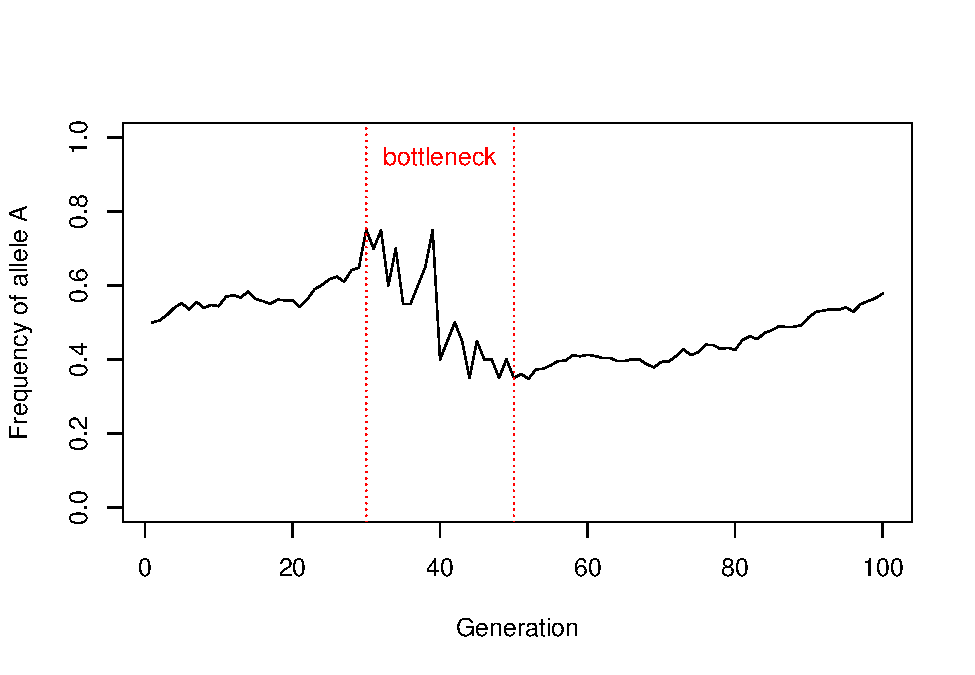
\includegraphics[keepaspectratio,alt={\label{fig:bottlenecksimulationplot}Simulation of a genetic bottleneck: 1000 individuals, falling to 10 individuals in generations 30 to 50}]{BB512_files/BB512_files/figure-latex/bottlenecksimulationplot-1.pdf}}
\caption{\label{fig:bottlenecksimulationplot}Simulation of a genetic bottleneck: 1000 individuals, falling to 10 individuals in generations 30 to 50}
\end{figure}

Run the bottleneck simulation several times, and answer the following questions:

\begin{itemize}
\tightlist
\item
  How does a genetic bottleneck influence the genetic composition of the population?
\item
  How might a genetic bottleneck affect the probability that one allele is fixed and the other lost?
\item
  What happens to allele frequency \emph{after} the bottleneck, when the population is large again? Does the population ``recover'' its original allele frequency?
\item
  Does the severity of the bottleneck (i.e.~its length and the population size during it) matter?
\end{itemize}

\subsection{Founder effects}\label{founder-effects}

A founder effect is like a bottleneck at the very start of a new population. To simulate it, take a large source population (1000 individuals, frequency of \emph{A} = 0.5) and found a new population from just 10 individuals (20 alleles) drawn at random from it. Repeat this 50 times, as if 50 islands were each colonised by a different group of 10 founders:

\begin{Shaded}
\begin{Highlighting}[]
\NormalTok{source\_pool }\OtherTok{\textless{}{-}} \FunctionTok{c}\NormalTok{(}\FunctionTok{rep}\NormalTok{(}\StringTok{"A"}\NormalTok{, }\DecValTok{1000}\NormalTok{), }\FunctionTok{rep}\NormalTok{(}\StringTok{"a"}\NormalTok{, }\DecValTok{1000}\NormalTok{))}

\NormalTok{founder\_freq\_A }\OtherTok{\textless{}{-}} \FunctionTok{replicate}\NormalTok{(}\DecValTok{50}\NormalTok{, \{}
\NormalTok{  founders }\OtherTok{\textless{}{-}} \FunctionTok{sample}\NormalTok{(source\_pool, }\DecValTok{2} \SpecialCharTok{*} \DecValTok{10}\NormalTok{, }\AttributeTok{replace =} \ConstantTok{FALSE}\NormalTok{)}
  \FunctionTok{mean}\NormalTok{(founders }\SpecialCharTok{==} \StringTok{"A"}\NormalTok{)}
\NormalTok{\})}

\FunctionTok{hist}\NormalTok{(founder\_freq\_A, }\AttributeTok{breaks =} \FunctionTok{seq}\NormalTok{(}\DecValTok{0}\NormalTok{, }\DecValTok{1}\NormalTok{, }\AttributeTok{by =} \FloatTok{0.05}\NormalTok{),}
     \AttributeTok{xlab =} \StringTok{"Frequency of allele A in the founded population"}\NormalTok{,}
     \AttributeTok{main =} \StringTok{""}\NormalTok{)}
\FunctionTok{abline}\NormalTok{(}\AttributeTok{v =} \FloatTok{0.5}\NormalTok{, }\AttributeTok{col =} \StringTok{"red"}\NormalTok{, }\AttributeTok{lty =} \DecValTok{3}\NormalTok{)}
\end{Highlighting}
\end{Shaded}

\begin{figure}
\centering
\pandocbounded{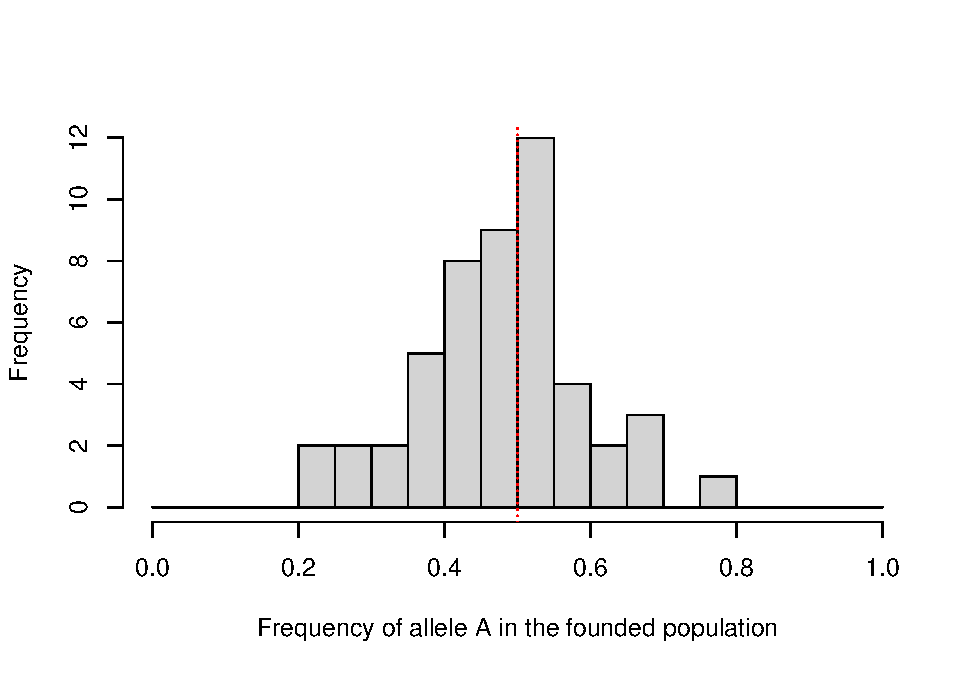
\includegraphics[keepaspectratio,alt={\label{fig:foundereffect}Frequency of allele A in 50 new populations, each founded by 10 individuals from a source population where the frequency of A is 0.5}]{BB512_files/BB512_files/figure-latex/foundereffect-1.pdf}}
\caption{\label{fig:foundereffect}Frequency of allele A in 50 new populations, each founded by 10 individuals from a source population where the frequency of A is 0.5}
\end{figure}

\begin{itemize}
\tightlist
\item
  How different are the new populations from the source population, and from each other?
\item
  How would this change with 50 founders instead of 10?
\item
  Optional: use \texttt{simulate\_gene\_pool()} with \texttt{initial\_freq\_A} set to one of these founder frequencies to follow a founded population forward in time.
\end{itemize}

\section{Conclusions}\label{conclusions}

You should now have a good idea of what a gene pool model is, the importance of population size, the concept of sampling from a population, and how bottlenecks and founder effects change genetic composition.

Let's finish with some more general questions:

\begin{itemize}
\tightlist
\item
  What are the limitations of this simulation? Look back at the list of assumptions in ``The model and its assumptions''. Which real-world processes and complexities are missing?
\item
  Why is genetic diversity important to a population, for example in a conservation context?
\item
  Can you think of real-life scenarios where understanding gene pool dynamics would be valuable, such as in conservation biology or medical genetics?
\end{itemize}

\section{Takeaways}\label{takeaways-14}

\begin{itemize}
\tightlist
\item
  Genetic drift is stronger in small populations because sampling error is larger.
\item
  Drift does not favour either allele: a neutral allele's probability of fixation equals its starting frequency. Population size changes how \emph{quickly} variation is lost.
\item
  Most new mutations (starting at \(1/(2N)\)) are lost by chance.
\item
  Bottlenecks and founder effects can rapidly reshape allele frequencies, and the change persists after the population becomes large again.
\end{itemize}

\textbf{Challenge:} Can you think of a way to simulate the genetics of a population that is steadily shrinking through time? Try it.

\chapter{Neutral or Adaptive Evolution in Humans: What Drives Evolution of Our Traits?}\label{neutral-or-adaptive-evolution-in-humans-what-drives-evolution-of-our-traits}

\section{Background}\label{background-14}

Understanding the role of natural selection and genetic drift in human traits requires a look at several key aspects:

\begin{itemize}
\tightlist
\item
  Heritable variation: a trait can only evolve (by drift or by selection) if individuals differ in it \emph{and} some of those differences are inherited.
\item
  Selection vs drift: selection acts when variation in a trait is correlated with variation in survival or reproduction. Drift is chance change in allele frequencies, and it acts in every finite population.
\item
  Role of environment: the environment can change the strength, and even the direction, of selection on a trait.
\end{itemize}

\textbf{First ask: is the variation heritable?} Some traits vary a lot but are hardly inherited at all. For example, the fine texture of the iris and the detailed ridge patterns (minutiae) of fingerprints differ even between identical twins: they are mostly the result of chance events during development. Variation like this cannot evolve by drift or by selection, because it is not passed on.

\textbf{Neutral and adaptive evolution are two ends of a continuum.} In the lecture on genetic drift we defined neutral evolution. Suppose a trait varies, individuals vary in reproductive success, and the trait is inherited, \emph{but} the trait is not (or only very weakly) correlated with reproductive success. The trait still evolves, but by chance: this is neutral evolution, caused by genetic drift. When the correlation between the trait and reproductive success is strong, we get adaptive evolution, caused by natural selection. Most traits lie somewhere in between.

Population size also decides where a trait sits on this continuum. Drift acts on the alleles that affect a trait, and its strength per generation is about \(1/(2N_e)\), where \(N_e\) is the effective population size. Selection on those alleles is effective only when the selective advantage, \(s\), is clearly larger than roughly \(1/(2N_e)\). So weak selection that is effective in a large population can be swamped by drift in a small one. Whether a trait evolves ``neutrally'' therefore depends on population size as well as on the environment.

When selection is moderate or strong, a trait tends to be held close to some optimal value (stabilising selection) or to change in a consistent direction (directional selection): adaptive evolution. When selection is weak or absent, the alleles that affect the trait change in frequency at random, and the trait drifts: neutral evolution. Both require heritable variation to begin with: if there is little heritable variation, the trait will not respond much even if selection is strong.

Finally, the strength of selection depends on the environment. A trait may be important in some environments but not others, and may be selected for in one environment but against in another. For example, the skin pigment melanin protects against intense ultraviolet (UV) radiation, including UV damage to the vitamin folate, so darker skin is favoured where UV is intense. Where UV is weak, lighter skin allows more vitamin D to be made in the skin (Jablonski \& Chaplin 2010, \emph{PNAS}). Ancient DNA shows that some of the main light-skin alleles became common in Europe only within roughly the last 8,000 years (Mathieson et al.~2015, \emph{Nature}). Exactly which selective pressures mattered most, and when, is still debated.

The objective of this exercise is to develop an intuitive understanding of the effect of selection and genetic drift on traits.

\begin{figure}

{\centering 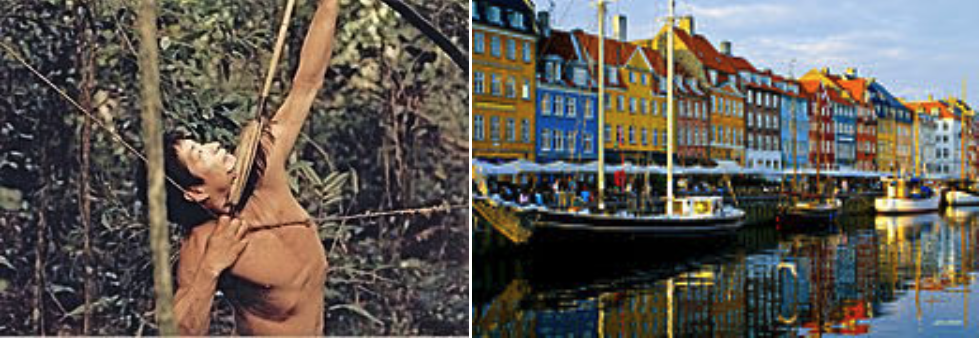
\includegraphics[width=0.5\linewidth]{images/huntergathererDK} 

}

\caption{Two present-day human environments: a forest where people hunt and gather (left) and a modern city, Copenhagen (right). Both photographs show people living today: all living human populations are equally evolved, and all are still subject to natural selection. How would selection on each trait differ between these environments?}\label{fig:huntergatherer}
\end{figure}

Learning outcomes:

\begin{itemize}
\tightlist
\item
  Decide whether a trait can evolve at all, by asking whether its variation is heritable.
\item
  Place traits on the continuum from neutral evolution (genetic drift) to adaptive evolution (natural selection), and justify each placement with evidence or reasoning.
\item
  Explain how the environment (foraging societies vs modern industrialised countries such as Denmark) and population size change the strength of selection on a trait.
\item
  Predict which differences between human populations gene flow would erase, and which local selection could maintain.
\item
  Use correct scientific terminology when arguing for your categorisation in a group.
\end{itemize}

\section{Key idea}\label{key-idea}

Traits like resistance to infectious disease are likely to face strong selection in environments where the disease is common. Heritable variation with little or no effect on survival or reproduction (for example, many DNA differences at synonymous sites, which do not change the protein) is more likely to change by drift.

\section{Evidence cards: some well-studied human cases}\label{evidence-cards-some-well-studied-human-cases}

These five cases have strong genetic evidence. Use them as reference points when you place the other traits.

\textbf{Lactase persistence (digesting milk sugar as an adult).} This is caused by variants near the \emph{LCT} gene that keep the lactase enzyme switched on in adults. \emph{Different} variants have arisen and spread in Europe, East Africa and the Middle East, in populations that keep milk-producing animals (Tishkoff et al.~2007, \emph{Nature Genetics}). They carry some of the strongest signals of recent selection in the human genome. Ancient DNA shows that the main European variant was rare until the last few thousand years. Why selection was so strong is still debated: milk drinking alone may not explain it, and famine and disease may have intensified it (Evershed et al.~2022, \emph{Nature}).

\textbf{EDAR V370A.} This is a single amino-acid change in the \emph{EDAR} gene, common in East Asia and the Americas. It affects hair thickness, sweat gland density and tooth shape, and it shows a strong signal of past selection (Kamberov et al.~2013, \emph{Cell}). Which of these traits (if any) was the target of selection is not known.

\textbf{Malaria resistance: HbS and Duffy-null.} People heterozygous for the sickle-cell allele (HbS) are protected against severe \emph{Plasmodium falciparum} malaria: heterozygote advantage, as in the Hardy-Weinberg practical. The Duffy-null allele protects against \emph{Plasmodium vivax} malaria. It is close to fixation in much of sub-Saharan Africa but rare elsewhere, a pattern that suggests strong local selection (Hamblin \& Di Rienzo 2000, \emph{American Journal of Human Genetics}).

\textbf{ABO blood groups.} The A and B alleles are very old: the polymorphism is shared with other primates, which suggests that selection has \emph{maintained} variation for millions of years (balancing selection), probably through infectious diseases (Ségurel et al.~2012, \emph{PNAS}).

\textbf{Earwax type (wet or dry), \emph{ABCC11}.} A single DNA change determines dry earwax (Yoshiura et al.~2006, \emph{Nature Genetics}). The dry allele is common in East Asia and rare in Europe and Africa. There is a signal of selection (Ohashi et al.~2011, \emph{Molecular Biology and Evolution}), but the trait it acted on (perhaps sweat and body odour) is uncertain. This is a good example of a case where the honest answer is ``we don't fully know''.

\section{Your task (35 minutes)}\label{your-task-35-minutes}

You are given a list of traits for humans (below). In small groups:

\begin{enumerate}
\def\labelenumi{\arabic{enumi}.}
\tightlist
\item
  Write the traits on PostIt notes, and read the evidence cards above (5 minutes).
\item
  Discuss and categorise the traits based on the strength of natural selection in foraging (hunter-gatherer) societies, like those in which most of human evolution took place (10 minutes).
\item
  Repeat the exercise for modern industrialised societies like Denmark (10 minutes). In Denmark today, most people survive to adulthood, so ask how each trait might affect the \emph{number of children} people have: selection still acts, but now mainly through differences in reproduction rather than survival.
\item
  \textbf{Gene flow between populations} (10 minutes). Human populations exchange migrants, and gene flow pulls their allele frequencies together. In the lecture on migration and gene flow we saw that very few migrants (about one per generation) are enough to stop drift making populations very different, but that local selection can keep populations different if it is strong compared with the migration rate (\(s\) larger than \(m\)). For each trait, ask:

  \begin{itemize}
  \tightlist
  \item
    Does the trait differ between human populations living in different environments?
  \item
    Would gene flow erase those differences (as expected for neutral traits), or could local selection hold them apart? Skin pigmentation and UV, lactase persistence and dairying, and HbS and malaria are good places to start.
  \item
    Remember that most human genetic variation is found \emph{within} populations rather than between them.
  \end{itemize}
\end{enumerate}

For steps 2 and 3, order the traits from those likely influenced by \textbf{GENETIC DRIFT} to those evolving through \textbf{ADAPTIVE EVOLUTION} via \textbf{NATURAL SELECTION}. For each trait, start with the question ``is the variation heritable?''.

\subsection{The traits}\label{the-traits}

{\def\LTcaptype{none} % do not increment counter
\begin{longtable}[]{@{}
  >{\raggedright\arraybackslash}p{(\linewidth - 2\tabcolsep) * \real{0.2613}}
  >{\raggedright\arraybackslash}p{(\linewidth - 2\tabcolsep) * \real{0.7387}}@{}}
\toprule\noalign{}
\begin{minipage}[b]{\linewidth}\raggedright
Trait
\end{minipage} & \begin{minipage}[b]{\linewidth}\raggedright
Description
\end{minipage} \\
\midrule\noalign{}
\endhead
\bottomrule\noalign{}
\endlastfoot
Metabolic efficiency & How effectively your body converts food into energy. \\
Amount of body hair & The density and length of hair covering your body. \\
Singing ability & Skill and aptitude for musical vocalisation. \\
Intelligence & Cognitive abilities including problem solving and learning (read the note below). \\
Eye colour & The colour of the iris (brown, green, blue and so on). \\
Earwax type & Wet or dry earwax (see the evidence cards). \\
Sperm motility & The movement and swimming of sperm. \\
Muscle strength & Physical power and force exerted by muscles. \\
Face symmetry & The balance and proportionality of facial features. \\
Running speed & How fast an individual can run. \\
Height & Physical stature, from base to top. \\
Birth canal (pelvic) shape & The shape of the bony opening through which a baby is born. \\
Resistance to bubonic plague & Immunity or resilience against bubonic plague. \\
Sense of smell & The ability to detect and identify odours. \\
Resistance to common cold & Immunity or resilience against the common cold. \\
Eyesight acuity & Sharpness of vision. \\
\end{longtable}
}

\textbf{A note on the intelligence trait.} Discuss only how selection might act on differences \emph{between individuals within} a population. Do not compare or rank human populations. A trait can be highly heritable within each of two groups, and yet the difference between the groups can be entirely environmental: heritability measured within a group says nothing about the causes of differences between groups (Neal, ``Polygenic Inheritance and Quantitative Genetics'', and the lecture on polygenic inheritance and quantitative genetics). The history of eugenics, which tried to ``improve'' human populations by stopping some people from having children, shows why this matters. It was ethically indefensible and, as the lecture on haploid and zygotic selection shows, genetically ineffective.

\section{Discussion (10 minutes)}\label{discussion-10-minutes}

After the exercise, discuss as a class:

\begin{itemize}
\tightlist
\item
  Were there any traits that were categorised differently between the two types of societies? Why?
\item
  Which traits did you decide had little or no heritable variation, and so could not evolve by drift or by selection?
\item
  Which differences between human populations would gene flow erase, and which are maintained by local selection?
\item
  Did the exercise challenge any preconceived notions you had about trait evolution?
\item
  Can you think of any other traits that would be interesting to add to this exercise?
\end{itemize}

\section{Takeaways}\label{takeaways-15}

\begin{itemize}
\tightlist
\item
  A trait can only evolve if its variation is heritable.
\item
  Neutral and adaptive evolution are two ends of a continuum: where a trait sits depends on how strongly it affects survival or reproduction, and on population size (\(s\) compared with \(1/(2N_e)\)).
\item
  Selection strength depends on environment and context, not just on the trait itself, and different environments can reverse which traits are favoured.
\item
  Humans are still evolving: in industrialised societies, selection acts mainly through differences in the number of children.
\item
  Gene flow erases neutral differences between populations, but local selection can maintain differences in traits such as skin pigmentation.
\end{itemize}

\chapter{Heritability from a linear regression}\label{heritability-from-a-linear-regression}

\section{Background}\label{background-15}

Heritability measures how much of the variation in a trait \textbf{within a population} is due to additive genetic differences between individuals. It is a proportion, between 0 and 1, and it tells us how closely offspring resemble their parents. Heritability matters in plant and animal breeding, in medicine and in conservation, because it determines how fast a trait can respond to selection.

Narrow-sense heritability is a ratio of two variances: the additive genetic variance divided by the total phenotypic variance.

\(h^2 = \frac{V_A}{V_P}\)

Only the additive part of the genetic variance counts, because parents pass on alleles, not whole genotypes. Effects that depend on particular combinations of alleles (dominance and interactions between genes) are broken up every generation, so they do not make offspring resemble their parents in a predictable way.

A heritability close to 1 means that most of the variation among individuals is additive genetic, so offspring closely resemble their parents. A heritability close to 0 means that parents' trait values tell us little about their offspring's: the variation is mostly due to the environment, to chance, or to non-additive genetic effects.

Heritability is not a fixed property of a trait. It belongs to a particular population in a particular environment, because it changes whenever either variance changes:

\begin{itemize}
\tightlist
\item
  \textbf{More environmental variation} (a patchier habitat, more variable weather or food) increases \(V_P\) and so lowers \(h^2\), even if \(V_A\) is unchanged.
\item
  \textbf{Selection} removes unfavourable alleles and so reduces \(V_A\). A trait under strong, persistent selection can end up with low heritability.
\item
  \textbf{Genetic architecture} (how many genes affect the trait, and how large their effects are) differs between traits and species.
\end{itemize}

We can estimate heritability from the resemblance between parents and offspring. If we plot the mean value of the offspring in each family against the \textbf{mid-parent value} (the mean of the two parents), the slope of the regression line estimates \(h^2\). If you only know one parent, the slope estimates \(h^2/2\), because each parent passes on only half of its alleles. This is the method used in the lecture for East's tobacco plants and for Darwin's finches.

\textbf{Reference}

\href{https://www.nature.com/scitable/topicpage/estimating-trait-heritability-46889/}{Wray, N. \& Visscher, P. (2008) Estimating trait heritability. Nature Education 1(1):29}

Learning Outcomes:

\begin{itemize}
\tightlist
\item
  Estimate narrow-sense heritability, with its uncertainty, from a mid-parent--offspring regression in R.
\item
  Use heritability and phenotypic variance to estimate additive genetic variance, and explain why heritability can differ between populations.
\item
  Evaluate the assumptions behind regression estimates of heritability.
\end{itemize}

\section{Before you start: predict}\label{before-you-start-predict-2}

Imagine plotting offspring wing length against mid-parent wing length.

\begin{itemize}
\tightlist
\item
  What slope would you expect if offspring were, on average, exactly like their parents?
\item
  What slope would you expect if offspring were no more like their own parents than like any other bird in the population?
\item
  What does a slope between these two tell you?
\end{itemize}

Write down your answers, then check them against your results at the end.

\section{Your Task}\label{your-task-15}

\subsection{Estimating heritability (15 minutes)}\label{estimating-heritability-15-minutes}

You are provided with two datasets for wing length (mm) in a small songbird. Each row is one family: \texttt{Midparent\_value} is the mean wing length of the two parents, and \texttt{Offspring\_value} is the wing length of one of their offspring, measured as an adult. Each dataset contains 100 families.

\href{https://www.dropbox.com/scl/fi/8oe1can46pshxojw1p29m/heritability_pop1.csv?rlkey=ssg6ymzr85gkrzw9e1y63ghzu&dl=0}{Data set 1}

\href{https://www.dropbox.com/scl/fi/yoy0x7kczvlr1eku5057m/heritability_pop2.csv?rlkey=30hta1di8v6w93ghbhq09dlbm&dl=0}{Data set 2}

\begin{enumerate}
\def\labelenumi{\arabic{enumi})}
\tightlist
\item
  Download the first data set and import it into R (RStudio). The starter code assumes you have saved it in a folder called \texttt{data} inside your project; change the path if you saved it somewhere else.
\item
  Plot the data, with mid-parent value on the x-axis and offspring value on the y-axis.
\item
  Fit a linear regression model of the form \texttt{y\ \textasciitilde{}\ x}.
\item
  Look at the slope of the relationship: this is your estimate of the heritability. Use \texttt{confint()} to find its 95\% confidence interval.
\end{enumerate}

Starter code in R:

\begin{Shaded}
\begin{Highlighting}[]
\NormalTok{pop\_1 }\OtherTok{\textless{}{-}} \FunctionTok{read.csv}\NormalTok{(}\StringTok{"data/Heritability\_Pop1.csv"}\NormalTok{)}
\FunctionTok{plot}\NormalTok{(pop\_1}\SpecialCharTok{$}\NormalTok{Midparent\_value, pop\_1}\SpecialCharTok{$}\NormalTok{Offspring\_value,}
     \AttributeTok{xlab =} \StringTok{"Mid{-}parent wing length (mm)"}\NormalTok{, }\AttributeTok{ylab =} \StringTok{"Offspring wing length (mm)"}\NormalTok{)}
\NormalTok{mod1 }\OtherTok{\textless{}{-}} \FunctionTok{lm}\NormalTok{(Offspring\_value }\SpecialCharTok{\textasciitilde{}}\NormalTok{ Midparent\_value, }\AttributeTok{data =}\NormalTok{ pop\_1)}
\FunctionTok{abline}\NormalTok{(mod1, }\AttributeTok{col =} \StringTok{"red"}\NormalTok{)}
\FunctionTok{summary}\NormalTok{(mod1)}
\FunctionTok{coef}\NormalTok{(mod1)[}\DecValTok{2}\NormalTok{]     }\CommentTok{\# slope = heritability estimate}
\FunctionTok{confint}\NormalTok{(mod1)[}\DecValTok{2}\NormalTok{, ] }\CommentTok{\# 95\% confidence interval for the slope}
\end{Highlighting}
\end{Shaded}

\textbf{Questions}

\begin{itemize}
\tightlist
\item
  What is your estimate of \(h^2\), and how precise is it?
\item
  What does this heritability tell us about the variation in wing length in this population? What does it \emph{not} tell us about any one bird?
\item
  What else might explain the remaining variation?
\item
  Calculate \(V_P\) as the variance of the offspring values (\texttt{var(pop\_1\$Offspring\_value)}). Why should we not use the variance of the mid-parent values for this? Then calculate the additive genetic variance, \(V_A = h^2 \times V_P\).
\item
  Imagine a breeder selects parents whose mean wing length is 2 mm above the population mean. Use the breeder's equation, \(R = h^2 S\), to predict the change in mean wing length in the next generation.
\end{itemize}

\subsection{Comparative Analysis (10 minutes)}\label{comparative-analysis-10-minutes}

Now analyse the second data set. It is for the same trait in the same species, but from a different population living in a different environment. Repeat steps 1 to 4, and calculate \(V_P\) and \(V_A\) for this population too.

\textbf{Questions}

\begin{itemize}
\tightlist
\item
  How does the heritability compare with population 1? Do the two confidence intervals overlap?
\item
  Compare \(V_P\) and \(V_A\) between the two populations. Which variance component differs, and what does that suggest about the cause of the difference in heritability?
\item
  Can you suggest environmental differences between the two populations that could explain this?
\item
  For the same selection differential (\(S\) = 2 mm), which population would respond faster to selection?
\item
  Can you think of any real-world applications where understanding heritability would be important?
\end{itemize}

\subsection{Assumptions (10 minutes)}\label{assumptions-10-minutes}

Estimating heritability from a mid-parent--offspring regression assumes the following.

\begin{itemize}
\tightlist
\item
  \textbf{Additive genetic effects:} the slope estimates the additive genetic variance only. Dominance and interactions between genes do not make offspring resemble parents, and the method does not account for genotype-by-environment interactions.
\item
  \textbf{No shared environment:} parents and offspring do not resemble each other for non-genetic reasons. If they share a territory, food supply or parental care, the heritability will be overestimated. Cross-fostering experiments (swapping eggs or chicks between nests) break this link.
\item
  \textbf{Correct parentage:} the measured parents are the genetic parents. In many birds, some chicks are sired by a male other than the social father (extra-pair paternity), which makes the heritability look lower than it is.
\item
  \textbf{Linearity:} the relationship between parent and offspring trait values is a straight line.
\item
  \textbf{Measurement accuracy:} measurement error in the parents' values makes the slope shallower, so heritability is underestimated; error in the offspring values makes the estimate less precise.
\item
  \textbf{Random mating:} mates do not choose each other on the basis of the trait (no assortative mating).
\item
  \textbf{Representative sample:} the families measured are a random sample of the population. If only some birds are sampled (for example, only those that survived a harsh winter), selection on the trait can bias the estimate.
\item
  \textbf{Independence:} each family contributes one data point. Using the same parents in several families, or several offspring from one family as separate data points, violates this.
\end{itemize}

\textbf{Question}

\begin{itemize}
\tightlist
\item
  For each assumption, how might it be violated in a wild bird population, and would that make the heritability estimate too high or too low?
\end{itemize}

\section{Takeaways}\label{takeaways-16}

\begin{itemize}
\tightlist
\item
  The slope of offspring on mid-parent estimates narrow-sense heritability, \(h^2 = V_A/V_P\); report it with its uncertainty.
\item
  Heritability belongs to a population in an environment: two populations with the same additive genetic variance can have very different heritabilities if their environments differ.
\item
  High heritability does not mean a trait is fixed or unaffected by the environment.
\end{itemize}

\chapter*{Part 4: Interactions Between Species and Community Structure}\label{part-4}
\addcontentsline{toc}{chapter}{Part 4: Interactions Between Species and Community Structure}

This part explores how species interactions shape population and community dynamics, using competition and predator-prey models.

By the end of Part 4, you should be able to:

\begin{itemize}
\tightlist
\item
  Interpret competition and predator-prey dynamics from model outputs.
\item
  Compare continuous- and discrete-time interaction models.
\item
  Reason about stability and equilibrium in multi-species systems.
\end{itemize}

\chapter{Lotka-Volterra competition}\label{lotka-volterra-competition}

The Lotka-Volterra competition model is a foundational tool in ecology for understanding interspecific competition, or competition between different species for shared resources such as food, space, and nesting sites. It examines how population sizes evolve in a shared environment by considering factors like interaction strength and environmental carrying capacities.

A key principle derived from this model is ``competitive exclusion'', which posits that two species with identical ecological roles can't coexist indefinitely. Eventually, one species will outcompete and exclude the other from the ecosystem.

The model also explores the role of both inter- and intra-specific competition. It identifies conditions for species coexistence, influenced by parameters like competition coefficients and carrying capacities. These insights are vital for understanding community structure, species interactions, and ecological stability.

In a two-species system there are four possible outcomes:

\begin{enumerate}
\def\labelenumi{\arabic{enumi}.}
\tightlist
\item
  \emph{Predictable Exclusion of Species 1 by Species 2:} Species 2 outcompetes and excludes species 1 from the environment.
\item
  \emph{Predictable Exclusion of Species 2 by Species 1:} Species 1 outcompetes and excludes species 2 from the environment.
\item
  \emph{Exclusion Dependent on Initial Densities:} Depending on the starting numbers of each species, either one could exclude the other.
\item
  \emph{Stable Coexistence:} Both species may reach a stable equilibrium where they coexist without one excluding the other.
\end{enumerate}

The model suggests that stable coexistence is possible if each species limits its own population growth more than it affects the other species. Overlapping niches could lead to competitive exclusion, influenced by their competition coefficients and carrying capacities.

Learning outcomes:

\begin{itemize}
\tightlist
\item
  Competence in constructing an Excel-based population model.
\item
  Understanding how the Lotka-Volterra competition model works.
\item
  Understanding the competition coefficients. These are called \(\alpha\) and \(\beta\) in the Neal textbook, and \(\alpha_{12}\) and \(\alpha_{21}\) in the PDF here.
\end{itemize}

\section{Key idea}\label{key-idea-1}

Whether a coefficient is bigger or smaller than 1 does not decide the outcome on its own. What matters is how each competition coefficient compares with the ratio of the carrying capacities. The easiest way to see this is to ask whether each species can invade when it is rare and the other species is sitting at its carrying capacity.

\begin{itemize}
\tightlist
\item
  Species 1 can invade a population of species 2 at \(K_2\) if \(K_1 > \alpha_{12} K_2\), i.e.~if \(\alpha_{12} < K_1/K_2\).
\item
  Species 2 can invade a population of species 1 at \(K_1\) if \(K_2 > \alpha_{21} K_1\), i.e.~if \(\alpha_{21} < K_2/K_1\).
\end{itemize}

{\def\LTcaptype{none} % do not increment counter
\begin{longtable}[]{@{}
  >{\raggedright\arraybackslash}p{(\linewidth - 4\tabcolsep) * \real{0.3333}}
  >{\raggedright\arraybackslash}p{(\linewidth - 4\tabcolsep) * \real{0.3333}}
  >{\raggedright\arraybackslash}p{(\linewidth - 4\tabcolsep) * \real{0.3333}}@{}}
\toprule\noalign{}
\begin{minipage}[b]{\linewidth}\raggedright
Species 1 can invade?
\end{minipage} & \begin{minipage}[b]{\linewidth}\raggedright
Species 2 can invade?
\end{minipage} & \begin{minipage}[b]{\linewidth}\raggedright
Outcome
\end{minipage} \\
\midrule\noalign{}
\endhead
\bottomrule\noalign{}
\endlastfoot
Yes & No & Species 1 excludes species 2 \\
No & Yes & Species 2 excludes species 1 \\
Yes & Yes & Stable coexistence \\
No & No & Exclusion, but which species wins depends on the starting densities \\
\end{longtable}
}

On the isocline graph, the same conditions appear as a comparison of the intercepts: \(K_1\) and \(K_1/\alpha_{12}\) for species 1, and \(K_2\) and \(K_2/\alpha_{21}\) for species 2.

For example, with \(K_1 = 3000\), \(\alpha_{12} = 1.25\), \(K_2 = 1000\) and \(\alpha_{21} = 0.5\), species 2 has the stronger per capita effect (\(\alpha_{12} > 1\)), yet species 1 wins: species 1 can invade (\(1.25 < 3000/1000 = 3\)) but species 2 cannot (\(0.5 > 1000/3000 = 0.33\)).

\section{Your task}\label{your-task-16}

In this class (over TWO sessions) you will be working from a PDF available \href{https://www.dropbox.com/s/oukr39oq0rsn8il/9.\%20Interspecific\%20Competition\%20and\%20Competitive\%20Exclusion.pdf?dl=1}{here} to make a model exploring this idea.

This PDF walks you through the creation of an Excel spreadsheet exploring interspecific competition and competitive exclusion using the Lotka-Volterra model.

\begin{itemize}
\tightlist
\item
  Create the Excel spreadsheet by following the instructions in the PDF
\end{itemize}

\textbf{Note on the PDF:} the labels added to Figure 5 have the subscripts the wrong way round. The correct isocline intercepts are \(K_1\) and \(K_1/\alpha_{12}\) for species 1, and \(K_2\) and \(K_2/\alpha_{21}\) for species 2 (as in the PDF text and the Key idea above).

\begin{itemize}
\tightlist
\item
  Use the Lotka-Volterra model you have created to answer the questions at the end of the PDF.
\end{itemize}

\subsection{The questions}\label{the-questions}

\begin{enumerate}
\def\labelenumi{\arabic{enumi}.}
\tightlist
\item
  What parameter values will cause species 1 to exclude species 2 from the habitat? What do these values mean in ecological terms?
\item
  What parameter values will reverse this outcome? What do these values mean in ecological terms?
\item
  What parameter values will allow the two species to coexist indefinitely and stably? What do these values mean in ecological terms?
\item
  Are there parameter values under which the outcome depends on initial population sizes or rates of population growth? What do these values mean in ecological terms?
\end{enumerate}

\section{Takeaways}\label{takeaways-17}

\begin{itemize}
\tightlist
\item
  Competition outcomes depend on relative self-limitation vs.~interspecific effects.
\item
  The competition coefficients \(\alpha_{12}\) and \(\alpha_{21}\) encode how much one species suppresses the other.
\item
  Coexistence occurs when each species limits itself more than it limits the other, in the scaled sense that \(\alpha_{12} < K_1/K_2\) and \(\alpha_{21} < K_2/K_1\) (each species can invade when rare). Comparing a coefficient with 1 is not enough when the carrying capacities differ.
\end{itemize}

\chapter{Lotka-Volterra predator-prey dynamics}\label{lotka-volterra-predator-prey-dynamics}

\section{Background}\label{background-16}

The Lotka-Volterra predator-prey model (Lotka 1925; Volterra 1926) is a fundamental concept in ecological dynamics, used to study the dynamics between predator and prey populations. Rosenzweig and MacArthur (1963) later extended this basic model to incorporate prey carrying capacity and predator functional response. The model assumes that the predator's population growth is directly influenced by the availability of its prey, while the prey's population growth is affected by predation pressure. As predator numbers increase, the prey population declines, which, in turn, leads to a decrease in predator numbers due to reduced food availability. This cyclical pattern continues as predator and prey populations oscillate over time.

The Lotka-Volterra predator-prey model gives us a framework for understanding the dynamics of species interactions.

In this class you will build and explore a Lotka-Volterra predator-prey model in Excel to gain insight into the ecology of interacting predators and prey.

Learning outcomes:

\begin{itemize}
\tightlist
\item
  Competence in constructing an Excel-based population model.
\item
  Understanding how the Lotka-Volterra predator-prey model works, and how it is visualised.
\end{itemize}

\section{Key idea}\label{key-idea-2}

The two isoclines (the lines where prey or predator numbers stop changing) are set by different parameters: the prey isocline by the prey's growth rate and the predator's attack rate, the predator isocline by the predator's death rate and how efficiently it turns prey into offspring. Changing a parameter moves an isocline, and so moves the equilibrium point where they cross. Whether the populations then cycle more or less widely depends on how far the starting numbers are from that new equilibrium.

\textbf{Important: the spreadsheet is a discrete-time model}

In the lecture, the Lotka-Volterra model is written in continuous time (dH/dt, dP/dt). In that model the populations cycle for ever: the cycles neither grow nor shrink (they are \emph{neutrally stable}), and their size depends only on the starting numbers.

The spreadsheet instead updates the populations once per time step (N(t+1) = N(t) + change over one step), like the discrete logistic model in \emph{Deeper into logistic growth}. Because each step uses the population sizes at the start of the step, the model always reacts a little too late, and the oscillations \textbf{grow} until one or both populations crash. This is a property of the discrete-time version (a time lag), not of predator-prey interactions in general.

Keep this in mind when you answer the questions below, especially question 6. You can compare the two versions in the R chapters \href{continuous-time-lotka-volterra-predator-prey-model-in-r.html}{Continuous-time Lotka-Volterra predator-prey model in R} and \href{discrete-time-lotka-volterra-predator-prey-model-in-r.html}{Discrete-time Lotka-Volterra predator-prey model in R}.

\section{Your task}\label{your-task-17}

Follow the PDF worksheet (\href{https://www.dropbox.com/s/bhwoe161wp9p6hp/10.\%20Predator-prey\%20dynamics.pdf?dl=1}{here}), which guides you to build and explore a Lotka-Volterra predator-prey model in Excel. The model has parameters for the prey and for the predator, and you will explore how these parameters influence the dynamics of the populations.

The worksheet is divided into four parts. We will mainly \textbf{focus on Part 1} - the basic model - in the class.

After completing the Excel sheet, try to answer the following questions:

\begin{enumerate}
\def\labelenumi{\arabic{enumi}.}
\tightlist
\item
  Does a larger prey population growth rate (R) increase or decrease the stability of the predator-prey interaction?
\item
  What happens if the predators starve more quickly? Less quickly?
\item
  What happens if the predator is more efficient at converting prey into offspring? Less efficient?
\item
  What happens if the predator is better at finding prey? Worse?
\item
  Is the behaviour of the model sensitive to starting populations? Begin with populations near the point where the isoclines cross, and move slowly farther out.
\item
  What is the ultimate outcome of the predator-prey interaction in the spreadsheet, regardless of parameter values? Is this outcome caused by the biology or by the model being discrete-time (see the box above)? How does this compare to real predator and prey populations? What factors not included in the model may explain the differences between model predictions and reality?
\end{enumerate}

\section{Optional extras}\label{optional-extras}

Part 2 modifies the basic model to include a refuge for the prey, part 3 adds a carrying capacity for the prey, and part 4 adds carrying capacities for both prey and predator. Feel free to continue to work on these if there is time, and if you are interested. Part 3 is particularly worth trying: prey self-limitation turns the expanding oscillations into damped ones that settle at an equilibrium.

\section{R-version}\label{r-version}

Two R versions are available: a \href{continuous-time-lotka-volterra-predator-prey-model-in-r.html}{continuous-time version} (the model in the lecture) and a \href{discrete-time-lotka-volterra-predator-prey-model-in-r.html}{discrete-time version} (the same model as this spreadsheet).

\subsection{References}\label{references}

Lotka, A. J. 1925. \emph{Elements of Physical Biology}. Williams \& Wilkins.

Volterra, V. 1926. Variazioni e fluttuazioni del numero d'individui in specie animali conviventi. \emph{Memorie della Reale Accademia Nazionale dei Lincei} 2: 31--113.

Rosenzweig, M. L. and R. H. MacArthur. 1963. Graphical representation and stability conditions of predator-prey interactions. \emph{American Naturalist} 97: 209--223.

\section{Takeaways}\label{takeaways-18}

\begin{itemize}
\tightlist
\item
  Predator-prey feedbacks can generate oscillations without external forcing.
\item
  Parameter changes move the isoclines and the equilibrium; in the continuous model the size of the cycles is set by the starting numbers.
\item
  The spreadsheet's growing oscillations come from its discrete time steps; the continuous model gives neutrally stable cycles.
\item
  Simple models highlight mechanisms but omit real-world constraints.
\end{itemize}

\chapter{Continuous-time Lotka-Volterra Predator-Prey Model in R}\label{continuous-time-lotka-volterra-predator-prey-model-in-r}

\section{Background}\label{background-17}

The Lotka-Volterra model describes the interaction between predators and prey. This document demonstrates how to program the continuous-time version of the model in R. Then, by varying the parameters you can explore its features, and visualise the dynamics of predator and prey populations over time.

Learning outcomes:

\begin{itemize}
\tightlist
\item
  Use of R to investigate an ecological model.
\item
  Understanding how the Lotka-Volterra predator-prey model works, and how it is visualised.
\end{itemize}

\section{What you should see}\label{what-you-should-see}

With the default parameters, you should see:

\begin{itemize}
\tightlist
\item
  repeating oscillations in predator and prey abundances through time, with the predator peaks following the prey peaks
\item
  a closed orbit in the phase plane around the coexistence equilibrium (the same loop is traced again and again)
\item
  straight-line isoclines (ZNGIs) whose intersection is the coexistence equilibrium
\end{itemize}

This is the same model as the Excel spreadsheet and the \href{discrete-time-lotka-volterra-predator-prey-model-in-r.html}{discrete-time R chapter}, with the same parameter values, but solved in continuous time. Comparing the three shows which behaviour belongs to the biology and which to the time steps.

\section{Your task}\label{your-task-18}

In R/RStudio, you will create an R script that programs the continuous time version of the Lotka-Volterra model. You will then use this model to investigate how the model works and how varying the parameters affects the system.

\subsection{Step 0: Create a new script}\label{step-0-create-a-new-script}

\begin{itemize}
\tightlist
\item
  Open RStudio and create a new script (File \textgreater{} New File \textgreater{} R Script).
\item
  Save it with a useful name (File \textgreater{} Save).
\item
  Type or copy/paste the following code, step-by-step, into the Script.
\item
  Run the code, or parts of it, selecting the parts you want to run and clicking ``Run''.
\end{itemize}

\subsection{Step 1: Load Necessary Libraries}\label{step-1-load-necessary-libraries}

We will use the \texttt{deSolve} package to solve the system of differential equations numerically. Note that you may need to install the package first using the command \texttt{install.packages("deSolve")}.

\begin{Shaded}
\begin{Highlighting}[]
\FunctionTok{library}\NormalTok{(deSolve)}
\end{Highlighting}
\end{Shaded}

\subsection{Step 2: Define the Model}\label{step-2-define-the-model}

The system of equations is defined as follows:

\begin{itemize}
\tightlist
\item
  Victim (prey) population growth: \(\frac{dV}{dt} = RV - aVC\)
\item
  Consumer (predator) population growth: \(\frac{dC}{dt} = afVC - qC\)
\end{itemize}

The function below implements these equations in R.

\begin{Shaded}
\begin{Highlighting}[]
\NormalTok{predator\_prey\_model }\OtherTok{\textless{}{-}} \ControlFlowTok{function}\NormalTok{(t, state, parameters) \{}
  \FunctionTok{with}\NormalTok{(}\FunctionTok{as.list}\NormalTok{(}\FunctionTok{c}\NormalTok{(state, parameters)), \{}
\NormalTok{    dV }\OtherTok{\textless{}{-}}\NormalTok{ R }\SpecialCharTok{*}\NormalTok{ V }\SpecialCharTok{{-}}\NormalTok{ a }\SpecialCharTok{*}\NormalTok{ V }\SpecialCharTok{*}\NormalTok{ C  }\CommentTok{\# Victim (prey) growth equation}
\NormalTok{    dC }\OtherTok{\textless{}{-}}\NormalTok{ a }\SpecialCharTok{*}\NormalTok{ f }\SpecialCharTok{*}\NormalTok{ V }\SpecialCharTok{*}\NormalTok{ C }\SpecialCharTok{{-}}\NormalTok{ q }\SpecialCharTok{*}\NormalTok{ C  }\CommentTok{\# Consumer (predator) growth equation}
    
    \FunctionTok{list}\NormalTok{(}\FunctionTok{c}\NormalTok{(dV, dC))}
\NormalTok{  \})}
\NormalTok{\}}
\end{Highlighting}
\end{Shaded}

\subsection{Step 3: Set Parameters and Initial Conditions}\label{step-3-set-parameters-and-initial-conditions}

We set the parameters and initial conditions for the model. I use the same nomenclature as the PDF from the \href{https://jonesor.github.io/BB512_Book/lotka-volterra-predator-prey-dynamics.html}{Excel exercise}, and the same values. The parameters are as follows: \emph{R} is the victim population growth rate, \emph{a} is the attack rate of the predator, \emph{f} is the conversion efficiency of the predator and \emph{q} is the predator starvation (death) rate. Here \emph{R} is an instantaneous rate (Neal's \emph{r}), because the model is in continuous time.

The Neal textbook (chapter \emph{Predator-Prey Interactions}) writes the same model as \(dH/dt = rH - aHP\) and \(dP/dt = cHP - dP\). The translation is: \(V = H\) (prey), \(C = P\) (predators), \(R = r\), \(a = a\), \(a \cdot f = c\) and \(q = d\).

\begin{Shaded}
\begin{Highlighting}[]
\NormalTok{parameters }\OtherTok{\textless{}{-}} \FunctionTok{c}\NormalTok{(}\AttributeTok{R =} \FloatTok{0.25}\NormalTok{, }\CommentTok{\# Victim (prey) growth rate}
                \AttributeTok{a =} \FloatTok{0.01}\NormalTok{, }\CommentTok{\# Attack rate}
                \AttributeTok{f =} \FloatTok{0.008}\NormalTok{, }\CommentTok{\# Conversion efficiency}
                \AttributeTok{q =} \FloatTok{0.1}\NormalTok{)  }\CommentTok{\# Predator death rate}

\NormalTok{initial\_state }\OtherTok{\textless{}{-}} \FunctionTok{c}\NormalTok{(}\AttributeTok{V =} \DecValTok{1000}\NormalTok{,  }\CommentTok{\# Initial victim population}
                   \AttributeTok{C =} \DecValTok{20}\NormalTok{)   }\CommentTok{\# Initial consumer population}
\end{Highlighting}
\end{Shaded}

\subsection{Step 4: Simulate the Model}\label{step-4-simulate-the-model}

We simulate the model over a specified time period and store the results.

\begin{Shaded}
\begin{Highlighting}[]
\NormalTok{time }\OtherTok{\textless{}{-}} \FunctionTok{seq}\NormalTok{(}\DecValTok{0}\NormalTok{, }\DecValTok{200}\NormalTok{, }\AttributeTok{by =} \FloatTok{0.1}\NormalTok{)  }\CommentTok{\# Time sequence}
\NormalTok{output }\OtherTok{\textless{}{-}} \FunctionTok{ode}\NormalTok{(}\AttributeTok{y =}\NormalTok{ initial\_state, }\AttributeTok{times =}\NormalTok{ time, }\AttributeTok{func =}\NormalTok{ predator\_prey\_model, }\AttributeTok{parms =}\NormalTok{ parameters)}
\NormalTok{output\_df }\OtherTok{\textless{}{-}} \FunctionTok{as.data.frame}\NormalTok{(output)}
\end{Highlighting}
\end{Shaded}

\subsection{Step 5: Visualise the Dynamics}\label{step-5-visualise-the-dynamics}

How does the size of the two populations change through time? You should see that the \textbf{amplitude} and \textbf{period} change as the parameters change.

\begin{itemize}
\tightlist
\item
  \textbf{Amplitude}: Half the difference between a population's peak and trough. It shows how much the population fluctuates.
\item
  \textbf{Period}: The time it takes for a population to complete one full cycle of oscillation. i.e.~the peak-to-peak distance. It indicates the speed of the population cycles.
\end{itemize}

\subsubsection{Population Dynamics Over Time}\label{population-dynamics-over-time}

The plot below shows the changes in consumer and victim populations over time.

\begin{Shaded}
\begin{Highlighting}[]
\CommentTok{\# Make room in the right{-}hand margin for the second axis label}
\FunctionTok{par}\NormalTok{(}\AttributeTok{mar =} \FunctionTok{c}\NormalTok{(}\DecValTok{5}\NormalTok{, }\DecValTok{4}\NormalTok{, }\DecValTok{4}\NormalTok{, }\DecValTok{5}\NormalTok{))}

\CommentTok{\# Plot victim population on the primary y{-}axis}
\FunctionTok{plot}\NormalTok{(output\_df}\SpecialCharTok{$}\NormalTok{time, output\_df}\SpecialCharTok{$}\NormalTok{V, }\AttributeTok{type =} \StringTok{"l"}\NormalTok{, }\AttributeTok{col =} \StringTok{"blue"}\NormalTok{, }\AttributeTok{lwd =} \DecValTok{2}\NormalTok{, }
     \AttributeTok{ylab =} \StringTok{"Victim Population (V)"}\NormalTok{, }\AttributeTok{xlab =} \StringTok{"Time"}\NormalTok{, }\AttributeTok{main =} \StringTok{"Predator{-}Prey Dynamics"}\NormalTok{)}

\CommentTok{\# Add consumer population on a secondary y{-}axis}
\FunctionTok{par}\NormalTok{(}\AttributeTok{new =} \ConstantTok{TRUE}\NormalTok{)}
\FunctionTok{plot}\NormalTok{(output\_df}\SpecialCharTok{$}\NormalTok{time, output\_df}\SpecialCharTok{$}\NormalTok{C, }\AttributeTok{type =} \StringTok{"l"}\NormalTok{, }\AttributeTok{col =} \StringTok{"red"}\NormalTok{, }\AttributeTok{lwd =} \DecValTok{2}\NormalTok{, }
     \AttributeTok{axes =} \ConstantTok{FALSE}\NormalTok{, }\AttributeTok{xlab =} \StringTok{""}\NormalTok{, }\AttributeTok{ylab =} \StringTok{""}\NormalTok{)}
\FunctionTok{axis}\NormalTok{(}\AttributeTok{side =} \DecValTok{4}\NormalTok{, }\AttributeTok{col =} \StringTok{"red"}\NormalTok{, }\AttributeTok{col.axis =} \StringTok{"red"}\NormalTok{)}
\FunctionTok{mtext}\NormalTok{(}\StringTok{"Consumer Population (C)"}\NormalTok{, }\AttributeTok{side =} \DecValTok{4}\NormalTok{, }\AttributeTok{line =} \DecValTok{3}\NormalTok{, }\AttributeTok{col =} \StringTok{"red"}\NormalTok{)}

\CommentTok{\# Add legend}
\FunctionTok{legend}\NormalTok{(}\StringTok{"topright"}\NormalTok{, }\AttributeTok{legend =} \FunctionTok{c}\NormalTok{(}\StringTok{"Victim (V)"}\NormalTok{, }\StringTok{"Consumer (C)"}\NormalTok{), }
       \AttributeTok{col =} \FunctionTok{c}\NormalTok{(}\StringTok{"blue"}\NormalTok{, }\StringTok{"red"}\NormalTok{), }\AttributeTok{lwd =} \DecValTok{2}\NormalTok{)}
\end{Highlighting}
\end{Shaded}

\pandocbounded{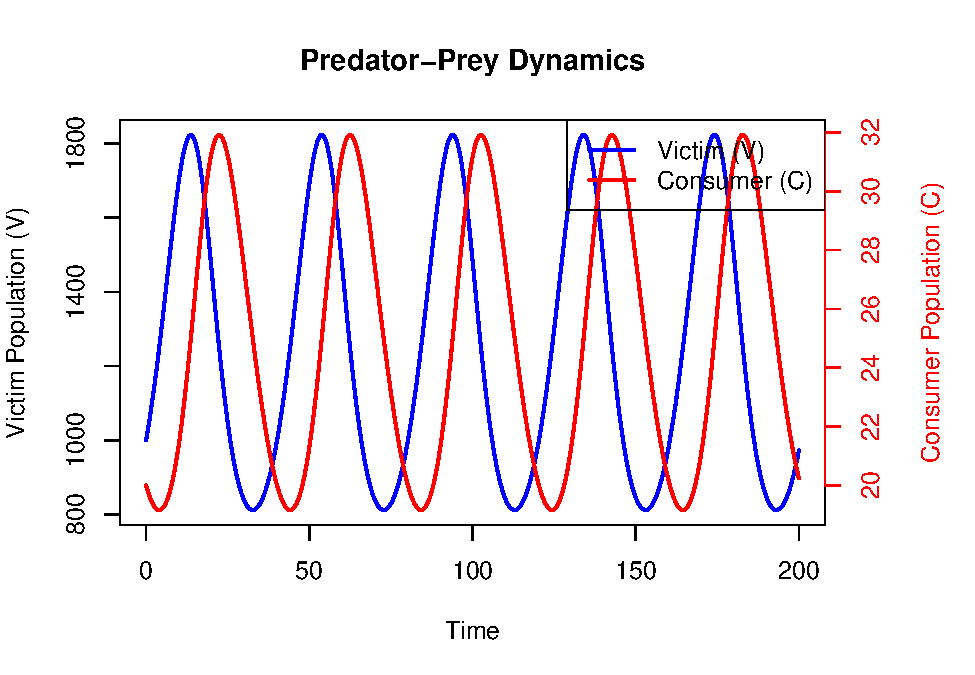
\includegraphics[keepaspectratio]{BB512_files/BB512_files/figure-latex/population-dynamics-1.pdf}}

\subsubsection{Phase Plot with ZNGIs}\label{phase-plot-with-zngis}

The phase plot shows the relationship between victim and consumer populations. Zero Net Growth Isoclines (ZNGIs) indicate where the growth rate of each population is zero.

\begin{Shaded}
\begin{Highlighting}[]
\FunctionTok{plot}\NormalTok{(output\_df}\SpecialCharTok{$}\NormalTok{V, output\_df}\SpecialCharTok{$}\NormalTok{C, }\AttributeTok{type =} \StringTok{"l"}\NormalTok{, }\AttributeTok{col =} \StringTok{"purple"}\NormalTok{, }\AttributeTok{lwd =} \DecValTok{2}\NormalTok{, }
     \AttributeTok{xlab =} \StringTok{"Victim (V)"}\NormalTok{, }\AttributeTok{ylab =} \StringTok{"Consumer (C)"}\NormalTok{, }
     \AttributeTok{main =} \StringTok{"Predator{-}Prey Dynamics with ZNGIs"}\NormalTok{)}

\CommentTok{\# Consumer ZNGI: dC/dt = 0 when V = q / (a * f) (a vertical line)}
\FunctionTok{abline}\NormalTok{(}\AttributeTok{v =}\NormalTok{ parameters[}\StringTok{"q"}\NormalTok{] }\SpecialCharTok{/}\NormalTok{ (parameters[}\StringTok{"a"}\NormalTok{] }\SpecialCharTok{*}\NormalTok{ parameters[}\StringTok{"f"}\NormalTok{]), }\AttributeTok{col =} \StringTok{"red"}\NormalTok{,}
       \AttributeTok{lwd =} \DecValTok{2}\NormalTok{, }\AttributeTok{lty =} \DecValTok{2}\NormalTok{)}
\CommentTok{\# Victim ZNGI: dV/dt = 0 when C = R / a (a horizontal line)}
\FunctionTok{abline}\NormalTok{(}\AttributeTok{h =}\NormalTok{ parameters[}\StringTok{"R"}\NormalTok{] }\SpecialCharTok{/}\NormalTok{ parameters[}\StringTok{"a"}\NormalTok{], }\AttributeTok{col =} \StringTok{"blue"}\NormalTok{, }\AttributeTok{lwd =} \DecValTok{2}\NormalTok{, }\AttributeTok{lty =} \DecValTok{2}\NormalTok{)}

\CommentTok{\# Add point for initial population sizes}
\FunctionTok{points}\NormalTok{(output\_df}\SpecialCharTok{$}\NormalTok{V[}\DecValTok{1}\NormalTok{], output\_df}\SpecialCharTok{$}\NormalTok{C[}\DecValTok{1}\NormalTok{], }\AttributeTok{pch =} \DecValTok{19}\NormalTok{, }\AttributeTok{col =} \StringTok{"black"}\NormalTok{, }\AttributeTok{cex =} \FloatTok{1.5}\NormalTok{)}

\CommentTok{\# Add an arrow to the end of the line}
\FunctionTok{arrows}\NormalTok{(}\AttributeTok{x0 =}\NormalTok{ output\_df}\SpecialCharTok{$}\NormalTok{V[}\FunctionTok{nrow}\NormalTok{(output\_df) }\SpecialCharTok{{-}} \DecValTok{1}\NormalTok{], }
       \AttributeTok{y0 =}\NormalTok{ output\_df}\SpecialCharTok{$}\NormalTok{C[}\FunctionTok{nrow}\NormalTok{(output\_df) }\SpecialCharTok{{-}} \DecValTok{1}\NormalTok{], }
       \AttributeTok{x1 =}\NormalTok{ output\_df}\SpecialCharTok{$}\NormalTok{V[}\FunctionTok{nrow}\NormalTok{(output\_df)], }
       \AttributeTok{y1 =}\NormalTok{ output\_df}\SpecialCharTok{$}\NormalTok{C[}\FunctionTok{nrow}\NormalTok{(output\_df)], }
       \AttributeTok{col =} \StringTok{"purple"}\NormalTok{, }\AttributeTok{length =} \FloatTok{0.1}\NormalTok{, }\AttributeTok{lwd =} \DecValTok{2}\NormalTok{)}
\end{Highlighting}
\end{Shaded}

\pandocbounded{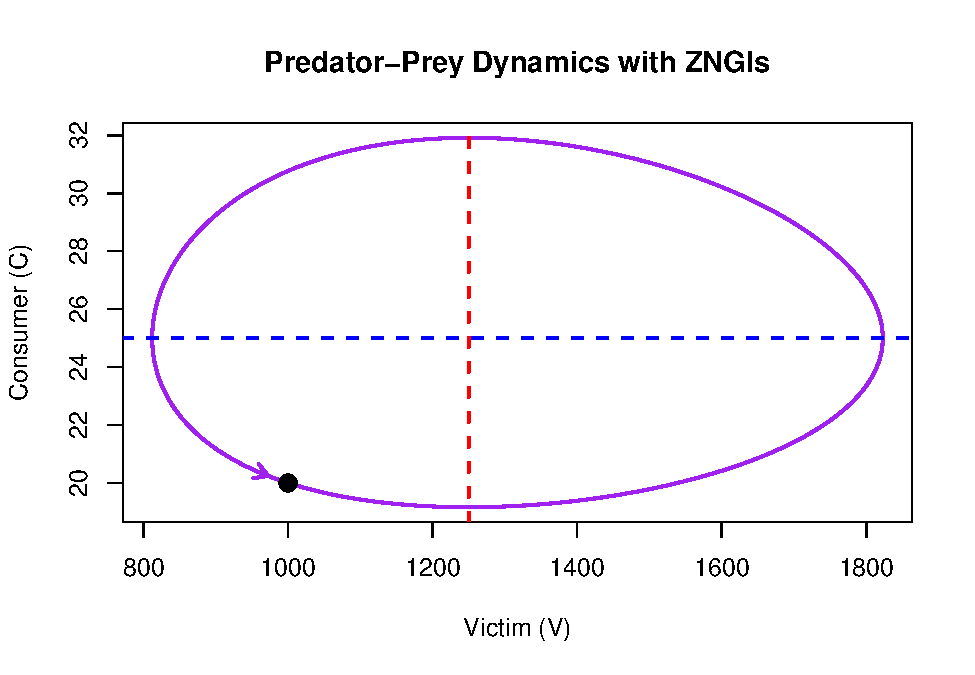
\includegraphics[keepaspectratio]{BB512_files/BB512_files/figure-latex/phase-plot-1.pdf}}

\subsection{Questions}\label{questions-11}

Before you change anything, write down a prediction for each question (a sentence or a quick sketch), then run the code to check it.

\textbf{1. Oscillations}

\begin{itemize}
\tightlist
\item
  Run the simulation with the default parameters. Describe how the two populations change through time. Which peaks first, prey or predators, and why?
\item
  In the phase plot, which way does the orbit go round (clockwise or anticlockwise)? Explain the direction using the four regions marked out by the isoclines.
\end{itemize}

\textbf{2. Neutral stability and starting numbers}

\begin{itemize}
\tightlist
\item
  \emph{Predict:} what will happen if you start exactly at the equilibrium, \(V = 1250\), \(C = 25\)? And just next to it, at \(V = 1300\), \(C = 25\)?
\item
  Now try starting values further away, e.g.~\(V = 2000, C = 20\) and \(V = 1000, C = 40\). What happens to the \emph{amplitude} and the \emph{period}? Do the oscillations grow, shrink or stay the same over time?
\end{itemize}

\textbf{3. Equilibrium and time-averages}

\begin{itemize}
\tightlist
\item
  Calculate the equilibrium for the default parameters, using
  \[
  V^* = \frac{q}{a \cdot f}, \quad C^* = \frac{R}{a}.
  \]
\item
  The populations never settle at these values. Instead, compare them with the \emph{average} population sizes over the simulation: \texttt{mean(output\_df\$V)} and \texttt{mean(output\_df\$C)}. What do you find?
\end{itemize}

\textbf{4. Moving the isoclines}

\begin{itemize}
\tightlist
\item
  \emph{Predict} which isocline (prey or predator) moves, and in which direction, if you double each of \(R\), \(a\), \(f\) and \(q\) in turn. Check your predictions on the phase plot.
\item
  A pesticide kills both prey and predators: it lowers \(R\) and raises \(q\). Try \(R = 0.2\) and \(q = 0.12\). What happens to the \emph{average} numbers of prey and predators? Is this what you would have guessed? (This is Volterra's principle; see Neal's \emph{Predator-Prey Interactions}.)
\end{itemize}

\textbf{5. Extinction and reality}

\begin{itemize}
\tightlist
\item
  Start far from the equilibrium, at \(V = 1000\), \(C = 100\). What are the smallest prey and predator numbers reached? Can either population reach exactly zero in this model? What would happen to a real population at these numbers?
\item
  Which assumptions of the model are unrealistic? Which real-world factors might stop the cycles continuing for ever?
\end{itemize}

\subsection{Conclusion}\label{conclusion}

This document demonstrates how to implement and explore the Lotka-Volterra predator-prey model in continuous time using R. By varying parameters and initial conditions, you can investigate how predator-prey dynamics are influenced by ecological factors. Notice that, unlike the discrete-time model (which has an implicit time lag of one time step and gives oscillations of increasing amplitude that end in extinction), the continuous-time model gives \emph{neutrally stable} cycles: they neither grow nor shrink, and their size depends on the starting populations. To see the discrete-time version, take a look at the Excel exercise (\href{https://jonesor.github.io/BB512_Book/lotka-volterra-predator-prey-dynamics.html}{here}) or the R exercise \href{discrete-time-lotka-volterra-predator-prey-model-in-r.html}{here}.

The main findings of the continuous time model are as follows:

\begin{enumerate}
\def\labelenumi{\arabic{enumi}.}
\item
  \textbf{Oscillatory Dynamics}: Predator and prey populations exhibit cyclical oscillations. The prey population increases when predator numbers are low, while the predator population grows when prey is abundant, so predator peaks follow prey peaks.
\item
  \textbf{Neutral Stability}: The oscillations are neutrally stable. They persist indefinitely without damping or amplification, and each pair of starting numbers gives its own orbit: the further from equilibrium you start, the larger the cycles. In the model neither population can ever reach exactly zero, but large orbits can take a population down to a fraction of one individual (for example, starting at \(V = 1000\), \(C = 100\) the predators fall to about 2 and the prey to about 8; with \(q = 1\) the predators fall to about 0.01). In a real population that would mean extinction.
\item
  \textbf{Equilibrium Points}: There are two equilibria:

  \begin{itemize}
  \tightlist
  \item
    The trivial equilibrium, where both predator and prey populations are zero.
  \item
    The coexistence equilibrium, \(V^* = q/(af)\) and \(C^* = R/a\). The populations cycle around it rather than settling at it, but the average population sizes over a cycle equal the equilibrium values.
  \end{itemize}
\item
  \textbf{Parameter Dependence}: The parameters set the position of the isoclines, and so the equilibrium: \(R\) and \(a\) move the prey isocline, \(q\), \(a\) and \(f\) move the predator isocline. The \emph{amplitude} of the cycles is set by how far the starting numbers are from the equilibrium. For small cycles the \emph{period} is approximately \(2\pi/\sqrt{Rq}\) (about 40 time units with the default parameters); large cycles take longer.
\item
  \textbf{Phase Plane Behaviour}: Predator and prey populations follow closed orbits in the phase plane around the coexistence equilibrium, anticlockwise when prey are on the x-axis, under the assumption that the system remains undisturbed.
\end{enumerate}

\section{Takeaways}\label{takeaways-19}

\begin{itemize}
\tightlist
\item
  Continuous-time predator-prey models generate sustained, neutrally stable cycles: their size is set by the starting numbers, not by the parameters alone.
\item
  Equilibria and isoclines help explain why cycles form and how parameters shift them; the average population sizes over a cycle equal the equilibrium.
\item
  Real ecosystems add damping, delays, and noise that change these dynamics.
\end{itemize}

\chapter{Discrete-time Lotka-Volterra Predator-Prey Model in R}\label{discrete-time-lotka-volterra-predator-prey-model-in-r}

Learning outcomes:

\begin{itemize}
\tightlist
\item
  Implement and explore a discrete-time predator-prey model in R.
\item
  Understand how time steps introduce delays and affect stability.
\item
  Compare discrete-time dynamics to continuous-time dynamics.
\end{itemize}

\section{Key idea}\label{key-idea-3}

With \(\Delta t = 1\), the phase plane typically shows expanding spirals, reflecting instability introduced by discrete time steps.

\section{Introduction}\label{introduction-1}

The Lotka-Volterra model describes the interaction between predators and prey. This document demonstrates how to program the discrete-time version of the model in R, explore its features, and visualise the dynamics of predator and prey populations over time. The time step (\(\Delta t\)) can be adjusted to explore the impact of a time delay in the system. In ecological systems, time delays can represent biological processes such as the time it takes for predators to respond to changes in prey density, for prey populations to recover after predation. If \(\Delta t\) is set to 1, this model is equivalent to a year-by-year model (as we have fitted in Excel in class), where the impact of predators on prey has a 1 year lag. i.e.~the growth of predators, depends on the availability of prey 1 year ago and the growth of prey depends on the amount of predators 1 year ago.

There are two ways to think about \(\Delta t\). With \(\Delta t = 1\) this is a model of populations that really do change in steps (e.g.~one breeding season per year). With \(\Delta t\) very small, nothing biological has changed: we are simply calculating the continuous-time model more accurately, in many small steps. The parameters and the starting numbers are the same as in the Excel spreadsheet and the \href{continuous-time-lotka-volterra-predator-prey-model-in-r.html}{continuous-time R chapter}.

\section{Step 1: Define the Model}\label{step-1-define-the-model}

The discrete-time equations are as follows:

\begin{itemize}
\item
  Victim (prey) population growth:\\
  \(V_{t+1} = V_t + \Delta t \cdot (R \cdot V_t - a \cdot C_t \cdot V_t)\)
\item
  Consumer (predator) population growth:\\
  \(C_{t+1} = C_t + \Delta t \cdot (a \cdot f \cdot V_t \cdot C_t - q \cdot C_t)\)
\end{itemize}

Note that, when \(\Delta t = 1\), the model is as follows:

\begin{itemize}
\item
  Victim (prey) population growth:\\
  \(V_{t+1} = V_t + R \cdot V_t - a \cdot C_t \cdot V_t\)
\item
  Consumer (predator) population growth:\\
  \(C_{t+1} = C_t + a \cdot f \cdot V_t \cdot C_t - q \cdot C_t\)
\end{itemize}

Compare these to Equations 1 and 2 in the Excel exercise PDF.

The function below implements these equations in R.

\begin{Shaded}
\begin{Highlighting}[]
\NormalTok{discrete\_predator\_prey\_model }\OtherTok{\textless{}{-}} \ControlFlowTok{function}\NormalTok{(time\_steps, dt, initial\_state, parameters) \{}
  \CommentTok{\# Initialise vectors to store populations}
\NormalTok{  time\_steps }\OtherTok{\textless{}{-}} \FunctionTok{round}\NormalTok{(time\_steps)}
\NormalTok{  V }\OtherTok{\textless{}{-}} \FunctionTok{numeric}\NormalTok{(time\_steps }\SpecialCharTok{+} \DecValTok{1}\NormalTok{)}
\NormalTok{  C }\OtherTok{\textless{}{-}} \FunctionTok{numeric}\NormalTok{(time\_steps }\SpecialCharTok{+} \DecValTok{1}\NormalTok{)}
\NormalTok{  time }\OtherTok{\textless{}{-}} \FunctionTok{seq}\NormalTok{(}\DecValTok{0}\NormalTok{, time\_steps }\SpecialCharTok{*}\NormalTok{ dt, }\AttributeTok{by =}\NormalTok{ dt)}
  
  \CommentTok{\# Set initial populations}
\NormalTok{  V[}\DecValTok{1}\NormalTok{] }\OtherTok{\textless{}{-}}\NormalTok{ initial\_state[}\StringTok{"V"}\NormalTok{]}
\NormalTok{  C[}\DecValTok{1}\NormalTok{] }\OtherTok{\textless{}{-}}\NormalTok{ initial\_state[}\StringTok{"C"}\NormalTok{]}
  
  \CommentTok{\# Extract parameters}
\NormalTok{  R }\OtherTok{\textless{}{-}}\NormalTok{ parameters[}\StringTok{"R"}\NormalTok{]}
\NormalTok{  a }\OtherTok{\textless{}{-}}\NormalTok{ parameters[}\StringTok{"a"}\NormalTok{]}
\NormalTok{  f }\OtherTok{\textless{}{-}}\NormalTok{ parameters[}\StringTok{"f"}\NormalTok{]}
\NormalTok{  q }\OtherTok{\textless{}{-}}\NormalTok{ parameters[}\StringTok{"q"}\NormalTok{]}
  
  \CommentTok{\# Loop through time steps to calculate populations}
  \ControlFlowTok{for}\NormalTok{ (t }\ControlFlowTok{in} \DecValTok{1}\SpecialCharTok{:}\NormalTok{time\_steps) \{}
    \CommentTok{\# max(0, ...) stops populations going negative (like IF() in Excel)}
\NormalTok{    V[t }\SpecialCharTok{+} \DecValTok{1}\NormalTok{] }\OtherTok{\textless{}{-}} \FunctionTok{max}\NormalTok{(}\DecValTok{0}\NormalTok{, V[t] }\SpecialCharTok{+}\NormalTok{ dt }\SpecialCharTok{*}\NormalTok{ (R }\SpecialCharTok{*}\NormalTok{ V[t] }\SpecialCharTok{{-}}\NormalTok{ a }\SpecialCharTok{*}\NormalTok{ V[t] }\SpecialCharTok{*}\NormalTok{ C[t]))}
\NormalTok{    C[t }\SpecialCharTok{+} \DecValTok{1}\NormalTok{] }\OtherTok{\textless{}{-}} \FunctionTok{max}\NormalTok{(}\DecValTok{0}\NormalTok{, C[t] }\SpecialCharTok{+}\NormalTok{ dt }\SpecialCharTok{*}\NormalTok{ (a }\SpecialCharTok{*}\NormalTok{ f }\SpecialCharTok{*}\NormalTok{ V[t] }\SpecialCharTok{*}\NormalTok{ C[t] }\SpecialCharTok{{-}}\NormalTok{ q }\SpecialCharTok{*}\NormalTok{ C[t]))}
\NormalTok{  \}}
  
  \CommentTok{\# Combine results into a data frame}
  \FunctionTok{data.frame}\NormalTok{(}\AttributeTok{time =}\NormalTok{ time, }\AttributeTok{V =}\NormalTok{ V, }\AttributeTok{C =}\NormalTok{ C)}
\NormalTok{\}}
\end{Highlighting}
\end{Shaded}

\section{Step 2: Set Parameters and Initial Conditions}\label{step-2-set-parameters-and-initial-conditions}

We set the parameters, initial conditions, the total time to simulate (\texttt{total\_time}) and the time step (\(\Delta t\)). The number of steps is calculated from these, so that changing \(\Delta t\) always covers the same total time and the runs can be compared fairly.

\begin{Shaded}
\begin{Highlighting}[]
\NormalTok{parameters }\OtherTok{\textless{}{-}} \FunctionTok{c}\NormalTok{(}\AttributeTok{R =} \FloatTok{0.25}\NormalTok{,  }\CommentTok{\# Victim (prey) growth rate}
                \AttributeTok{a =} \FloatTok{0.01}\NormalTok{,  }\CommentTok{\# Attack rate}
                \AttributeTok{f =} \FloatTok{0.008}\NormalTok{, }\CommentTok{\# Conversion efficiency}
                \AttributeTok{q =} \FloatTok{0.1}\NormalTok{)   }\CommentTok{\# Consumer (predator) death rate}

\NormalTok{initial\_state }\OtherTok{\textless{}{-}} \FunctionTok{c}\NormalTok{(}\AttributeTok{V =} \DecValTok{1000}\NormalTok{,  }\CommentTok{\# Initial victim population}
                   \AttributeTok{C =} \DecValTok{20}\NormalTok{)    }\CommentTok{\# Initial consumer population}

\NormalTok{total\_time }\OtherTok{\textless{}{-}} \DecValTok{300}             \CommentTok{\# Total time to simulate}
\NormalTok{dt }\OtherTok{\textless{}{-}} \DecValTok{1}                       \CommentTok{\# Time step (dt), 1 = a standard discrete model}
\NormalTok{time\_steps }\OtherTok{\textless{}{-}}\NormalTok{ total\_time }\SpecialCharTok{/}\NormalTok{ dt }\CommentTok{\# Number of time steps needed to cover total\_time}
\end{Highlighting}
\end{Shaded}

\section{Step 3: Simulate the Model}\label{step-3-simulate-the-model}

We simulate the model for the specified parameters and time steps.

\begin{Shaded}
\begin{Highlighting}[]
\NormalTok{output\_df }\OtherTok{\textless{}{-}} \FunctionTok{discrete\_predator\_prey\_model}\NormalTok{(}\AttributeTok{time\_steps =}\NormalTok{ time\_steps, }\AttributeTok{dt =}\NormalTok{ dt, }
                                          \AttributeTok{initial\_state =}\NormalTok{ initial\_state, }
                                          \AttributeTok{parameters =}\NormalTok{ parameters)}
\end{Highlighting}
\end{Shaded}

\section{Step 4: Visualise the Dynamics}\label{step-4-visualise-the-dynamics}

\subsection{Population Dynamics Over Time}\label{population-dynamics-over-time-1}

The plot below shows the changes in consumer and victim populations over time.

\begin{Shaded}
\begin{Highlighting}[]
\CommentTok{\# Make room in the right{-}hand margin for the second axis label}
\FunctionTok{par}\NormalTok{(}\AttributeTok{mar =} \FunctionTok{c}\NormalTok{(}\DecValTok{5}\NormalTok{, }\DecValTok{4}\NormalTok{, }\DecValTok{4}\NormalTok{, }\DecValTok{5}\NormalTok{))}

\CommentTok{\# Plot victim population on the primary y{-}axis}
\FunctionTok{plot}\NormalTok{(output\_df}\SpecialCharTok{$}\NormalTok{time, output\_df}\SpecialCharTok{$}\NormalTok{V, }\AttributeTok{type =} \StringTok{"l"}\NormalTok{, }\AttributeTok{col =} \StringTok{"blue"}\NormalTok{, }\AttributeTok{lwd =} \DecValTok{2}\NormalTok{, }
     \AttributeTok{ylab =} \StringTok{"Victim Population (V)"}\NormalTok{, }\AttributeTok{xlab =} \StringTok{"Time"}\NormalTok{, }\AttributeTok{main =} \StringTok{"Discrete Predator{-}Prey Dynamics"}\NormalTok{)}

\CommentTok{\# Add consumer population on a secondary y{-}axis}
\FunctionTok{par}\NormalTok{(}\AttributeTok{new =} \ConstantTok{TRUE}\NormalTok{)}
\FunctionTok{plot}\NormalTok{(output\_df}\SpecialCharTok{$}\NormalTok{time, output\_df}\SpecialCharTok{$}\NormalTok{C, }\AttributeTok{type =} \StringTok{"l"}\NormalTok{, }\AttributeTok{col =} \StringTok{"red"}\NormalTok{, }\AttributeTok{lwd =} \DecValTok{2}\NormalTok{, }
     \AttributeTok{axes =} \ConstantTok{FALSE}\NormalTok{, }\AttributeTok{xlab =} \StringTok{""}\NormalTok{, }\AttributeTok{ylab =} \StringTok{""}\NormalTok{)}
\FunctionTok{axis}\NormalTok{(}\AttributeTok{side =} \DecValTok{4}\NormalTok{, }\AttributeTok{col =} \StringTok{"red"}\NormalTok{, }\AttributeTok{col.axis =} \StringTok{"red"}\NormalTok{)}
\FunctionTok{mtext}\NormalTok{(}\StringTok{"Consumer Population (C)"}\NormalTok{, }\AttributeTok{side =} \DecValTok{4}\NormalTok{, }\AttributeTok{line =} \DecValTok{3}\NormalTok{, }\AttributeTok{col =} \StringTok{"red"}\NormalTok{)}

\CommentTok{\# Add legend}
\FunctionTok{legend}\NormalTok{(}\StringTok{"topright"}\NormalTok{, }\AttributeTok{legend =} \FunctionTok{c}\NormalTok{(}\StringTok{"Victim (V)"}\NormalTok{, }\StringTok{"Consumer (C)"}\NormalTok{), }
       \AttributeTok{col =} \FunctionTok{c}\NormalTok{(}\StringTok{"blue"}\NormalTok{, }\StringTok{"red"}\NormalTok{), }\AttributeTok{lwd =} \DecValTok{2}\NormalTok{)}
\end{Highlighting}
\end{Shaded}

\pandocbounded{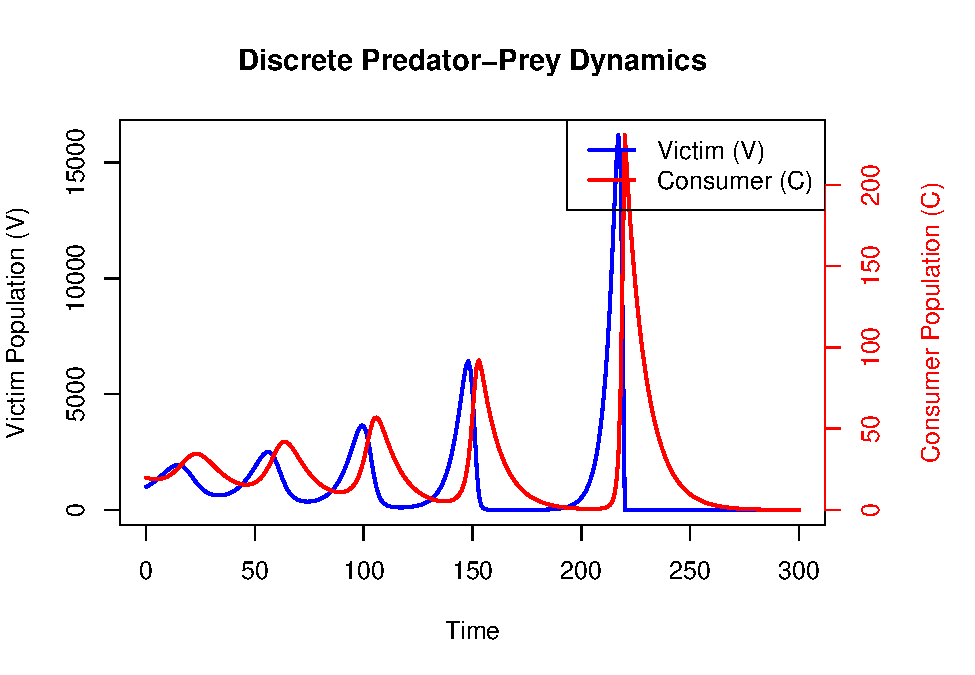
\includegraphics[keepaspectratio]{BB512_files/BB512_files/figure-latex/DT-population-dynamics-1.pdf}}

\subsection{Phase Plot with ZNGIs}\label{phase-plot-with-zngis-1}

The phase plot shows the relationship between victim and consumer populations.

\begin{Shaded}
\begin{Highlighting}[]
\DocumentationTok{\#\#\# Phase Plot with ZNGIs, Initial Point, and Arrow}
\FunctionTok{plot}\NormalTok{(output\_df}\SpecialCharTok{$}\NormalTok{V, }
\NormalTok{     output\_df}\SpecialCharTok{$}\NormalTok{C, }
     \AttributeTok{type =} \StringTok{"l"}\NormalTok{, }
     \AttributeTok{col =} \StringTok{"purple"}\NormalTok{, }
     \AttributeTok{lwd =} \DecValTok{2}\NormalTok{, }
     \AttributeTok{xlab =} \StringTok{"Victim (V)"}\NormalTok{, }\AttributeTok{ylab =} \StringTok{"Consumer (C)"}\NormalTok{, }
     \AttributeTok{main =} \StringTok{"Discrete Predator{-}Prey Dynamics with ZNGIs"}\NormalTok{)}

\CommentTok{\# Add Consumer ZNGI: no change in C when V = q / (a * f) (a vertical line)}
\FunctionTok{abline}\NormalTok{(}\AttributeTok{v =}\NormalTok{ parameters[}\StringTok{"q"}\NormalTok{] }\SpecialCharTok{/}\NormalTok{ (parameters[}\StringTok{"a"}\NormalTok{] }\SpecialCharTok{*}\NormalTok{ parameters[}\StringTok{"f"}\NormalTok{]),}
       \AttributeTok{col =} \StringTok{"red"}\NormalTok{, }\AttributeTok{lwd =} \DecValTok{2}\NormalTok{, }\AttributeTok{lty =} \DecValTok{2}\NormalTok{)}

\CommentTok{\# Add Victim ZNGI: no change in V when C = R / a (a horizontal line)}
\FunctionTok{abline}\NormalTok{(}\AttributeTok{h =}\NormalTok{ parameters[}\StringTok{"R"}\NormalTok{] }\SpecialCharTok{/}\NormalTok{ parameters[}\StringTok{"a"}\NormalTok{], }\AttributeTok{col =} \StringTok{"blue"}\NormalTok{, }\AttributeTok{lwd =} \DecValTok{2}\NormalTok{, }\AttributeTok{lty =} \DecValTok{2}\NormalTok{)}

\CommentTok{\# Add point for initial population sizes}
\FunctionTok{points}\NormalTok{(output\_df}\SpecialCharTok{$}\NormalTok{V[}\DecValTok{1}\NormalTok{], output\_df}\SpecialCharTok{$}\NormalTok{C[}\DecValTok{1}\NormalTok{], }\AttributeTok{pch =} \DecValTok{19}\NormalTok{, }\AttributeTok{col =} \StringTok{"black"}\NormalTok{, }\AttributeTok{cex =} \FloatTok{1.5}\NormalTok{)}

\CommentTok{\# Add an arrow to the end of the line}
\FunctionTok{arrows}\NormalTok{(}\AttributeTok{x0 =}\NormalTok{ output\_df}\SpecialCharTok{$}\NormalTok{V[}\FunctionTok{nrow}\NormalTok{(output\_df) }\SpecialCharTok{{-}} \DecValTok{1}\NormalTok{], }
       \AttributeTok{y0 =}\NormalTok{ output\_df}\SpecialCharTok{$}\NormalTok{C[}\FunctionTok{nrow}\NormalTok{(output\_df) }\SpecialCharTok{{-}} \DecValTok{1}\NormalTok{], }
       \AttributeTok{x1 =}\NormalTok{ output\_df}\SpecialCharTok{$}\NormalTok{V[}\FunctionTok{nrow}\NormalTok{(output\_df)], }
       \AttributeTok{y1 =}\NormalTok{ output\_df}\SpecialCharTok{$}\NormalTok{C[}\FunctionTok{nrow}\NormalTok{(output\_df)], }
       \AttributeTok{col =} \StringTok{"purple"}\NormalTok{, }\AttributeTok{length =} \FloatTok{0.1}\NormalTok{, }\AttributeTok{lwd =} \DecValTok{2}\NormalTok{)}
\end{Highlighting}
\end{Shaded}

\pandocbounded{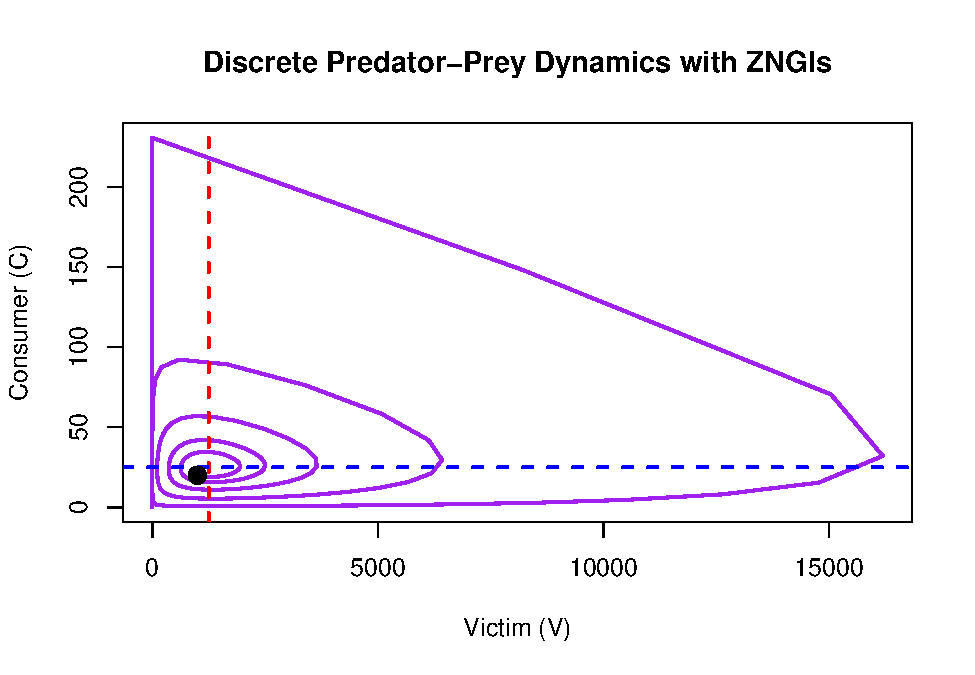
\includegraphics[keepaspectratio]{BB512_files/BB512_files/figure-latex/DT-phase-plot-1.pdf}}

\section{Your task}\label{your-task-19}

Before each run, predict what you will see (sketch the phase plot), then check.

\begin{itemize}
\tightlist
\item
  Run the model with the default settings (\(\Delta t = 1\), \texttt{total\_time\ =\ 300}). How does the phase plot differ from the closed orbit in the continuous-time chapter? When does the first population hit zero? Find it with \texttt{output\_df\$time{[}which(output\_df\$C\ ==\ 0\ \textbar{}\ output\_df\$V\ ==\ 0){[}1{]}{]}}.
\item
  Decrease \(\Delta t\) to 0.1 (keep \texttt{total\_time\ =\ 300}; the number of steps is recalculated for you, so re-run the parameter chunk as well as the simulation) and compare the phase plane behaviour to \(\Delta t = 1\). Then try \(\Delta t = 0.01\).
\item
  Increase \(\Delta t\) to 2 and observe whether extinction happens faster.
\item
  Change \(R\) or \(q\) (e.g.~double one of them) with \(\Delta t = 1\). Does the spiral grow faster or slower? Now double \(a\) or \(f\) instead. Which parameters control how quickly the spiral grows? (Careful: changing \(a\) or \(f\) also moves the equilibrium, so the default start is then nearer to or further from it. Compare how fast the spiral widens, not only when it ends.)
\end{itemize}

\section{Conclusion}\label{conclusion-1}

This document demonstrates how to implement and explore the discrete-time Lotka-Volterra predator-prey model. By adjusting the time step (\(\Delta t\)) and other parameters, you can investigate how predator-prey dynamics are influenced by ecological factors. With the default settings (\(\Delta t = 1\)), the time lag of one step makes the phase plot spiral outwards: the cycles grow until the prey are wiped out (they hit zero at \(t = 220\)), after which the predators starve and dwindle towards zero. Smaller time steps make the spiral grow more slowly, and with \(\Delta t = 0.01\) the orbit is almost closed, like the continuous-time model. Larger time steps make it grow faster: with \(\Delta t = 2\) the prey hit zero at \(t = 142\). Contrast this with the perpetual (neutrally stable) oscillations you get with the continuous-time model.

\section{Takeaways}\label{takeaways-20}

\begin{itemize}
\tightlist
\item
  Discrete time steps destabilise the predator-prey cycles of the continuous-time model: the populations react one step too late, so each cycle overshoots a little more than the last.
\item
  Each time step, the distance from the equilibrium grows by a factor of about \(\sqrt{1 + \Delta t^2 R q}\). This depends on the prey growth rate, the predator death rate and the step length, but not on the attack rate or conversion efficiency. With the default values it is about 1.012 per step (roughly 1 \% per step).
\item
  Smaller \(\Delta t\) values bring the discrete model closer to the continuous-time behaviour.
\end{itemize}

\chapter*{Part 5: Animal behaviour, altruism and sexual selection}\label{part-5}
\addcontentsline{toc}{chapter}{Part 5: Animal behaviour, altruism and sexual selection}

This part uses game theory and behavioral models to explore how selection shapes strategies like aggression, cooperation, and mating behavior.

By the end of Part 5, you should be able to:

\begin{itemize}
\tightlist
\item
  Explain how payoffs influence behavioral strategies.
\item
  Use game-theoretic reasoning to interpret conflicts and cooperation.
\item
  Connect behavioral models to evolutionary outcomes.
\end{itemize}

\chapter{Game theory: Hawks and doves}\label{game-theory-hawks-and-doves}

\section{Background}\label{background-18}

Game theory analyses interactions in which the payoff of a choice depends on what others choose. Maynard Smith and Price (1973) brought it into biology as \emph{evolutionary} game theory, which does not assume that animals are rational. Instead, each individual follows a strategy, strategies are heritable, and payoffs are measured in fitness, so strategies that earn more spread through the population. One particularly fascinating example is the Hawk and Dove game. Representing two distinct strategies, the Hawk embodies aggression and assertiveness, always seeking to escalate conflicts and dominate opponents. On the other hand, the Dove adopts a more peaceful and conciliatory approach, aiming to avoid confrontations and achieve cooperative outcomes.

By studying the Hawk and Dove strategies we can gain insights into understanding the delicate balance between competition and cooperation, shedding light on the dynamics of conflicts and the evolution of cooperative behaviour in both the natural world and human societies.

The simple model unravels the intricacies of strategic decision-making, with profound implications across various fields, from biology and social sciences to economics and politics.

In this activity, you play the role of the strategies: you will play the hawk and dove game with a single partner and then with multiple partners to observe the hypothetical costs and benefits of antagonistic or cooperative behaviour, respectively. The whole class enters results into one shared, live spreadsheet as you play, so we can watch the class-wide patterns emerge on screen in real time, round by round, instead of waiting until after class to see what happened.

Learning outcomes:

\begin{itemize}
\tightlist
\item
  Understanding of the fundamental concepts of game theory and its application in analysing strategic interactions in competitive environments.
\item
  Ability to apply game theory concepts to real-world contexts in biology, or politics.
\item
  Appreciation of how simple models can be used to address complex biological or political decision making.
\item
  Practice generating a testable prediction from a simple model \emph{before} collecting data, then checking it against real, live class results.
\end{itemize}

\section{Worked example}\label{worked-example-8}

\subsection{Inputs}\label{inputs-6}

\begin{itemize}
\tightlist
\item
  Benefit: \(B = 4\)
\item
  Cost: \(C = 3\)
\end{itemize}

\subsection{Steps}\label{steps-6}

\begin{enumerate}
\def\labelenumi{\arabic{enumi}.}
\tightlist
\item
  Compute Hawk-Hawk payoff: \((B-C)/2\).
\item
  Compute Hawk-Dove payoff to Hawk: \(B\) (and 0 to Dove).
\item
  Compute Dove-Dove payoff: \(B/2\) to each player.
\end{enumerate}

\subsection{Output and interpretation}\label{output-and-interpretation-6}

Hawk-Hawk gives \(0.5\) each, Hawk-Dove gives \texttt{4} to Hawk and \texttt{0} to Dove, and Dove-Dove gives \texttt{2} each.

\textbf{Link to the lecture: when does a mix of Hawks and Doves evolve?}

The class game uses the lecture's payoff matrix with the display cost set to zero (\(D = 0\)). This is also the matrix in Neal's chapter ``Animal Behaviour, Altruism and Limiting Aggression'', where Dove-Dove pays \(B/2 - D\).

\begin{itemize}
\tightlist
\item
  If \(B > C\) (as today, \(B = 4\), \(C = 3\)), Hawk earns more than Dove whatever the opponent plays, so in a one-off encounter the evolutionarily stable strategy (ESS) is pure Hawk.
\item
  If \(C > B\), neither pure strategy is stable. The ESS is a mix, with Hawks at frequency \(p^* = B/C\), where Hawks and Doves earn the same on average. For example, with \(B = 4\) and \(C = 8\), \(p^* = 0.5\). (With a display cost, as in the lecture's worked example, \(p^* = (B/2 + D)/(C/2 + D)\), which gives 7/12.)
\end{itemize}

\section{Your task}\label{your-task-20}

Before the activity starts, review the cost-benefit payoff table below to understand how to score the game.

\section{The payoff table}\label{the-payoff-table}

The general payoff table looks like this (payoff to \textbf{Player 1}):

{\def\LTcaptype{none} % do not increment counter
\begin{longtable}[]{@{}lrr@{}}
\toprule\noalign{}
Player 1 ~Player 2 & Hawk & Dove \\
\midrule\noalign{}
\endhead
\bottomrule\noalign{}
\endlastfoot
Hawk & \((B-C)/2\) & \(B\) \\
Dove & \(0\) & \(B/2\) \\
\end{longtable}
}

You can determine the benefit by looking at the left column and choosing the row corresponding to the card you played. The box that corresponds to your partner's choice is in the top row. For this game, B equals four (4), and C equals three (3). So depending on the cards played, player one (i.e., you) would gain a score of two (2), four (4), zero (0), or one-half (0.5). Like this:

{\def\LTcaptype{none} % do not increment counter
\begin{longtable}[]{@{}lrr@{}}
\toprule\noalign{}
Player 1 ~Player 2 & Hawk & Dove \\
\midrule\noalign{}
\endhead
\bottomrule\noalign{}
\endlastfoot
Hawk & 0.5 & 4 \\
Dove & 0 & 2 \\
\end{longtable}
}

\subsection{What does theory predict?}\label{what-does-theory-predict}

Before you play, work through this with your partner.

Because B (4) is bigger than C (3), Hawk beats Dove \emph{no matter what your opponent plays}: against a Dove you get 4 (vs.~2 for playing Dove yourself), and against a Hawk you still get 0.5 (vs.~0 for playing Dove). So in a single, anonymous encounter, Hawk is the dominant strategy: theory predicts everyone should end up playing Hawk.

But notice that mutual Hawk-Hawk (0.5 each) is \emph{worse for both of you} than mutual Dove-Dove (2 each). That means this game has the same structure as the famous Prisoner's Dilemma, with Hawk playing the role of ``Defect''. One twist: if you and your partner take turns (Hawk/Dove one round, Dove/Hawk the next), you each average (4 + 0)/2 = 2 per round, exactly as much as mutual Dove-Dove. So with these payoffs, taking turns is just as good a way to ``cooperate''.

\begin{itemize}
\tightlist
\item
  \textbf{Prediction for Game Two} (a new partner every round, i.e.~effectively a series of one-off encounters): theory says Hawk should dominate and pay off best.
\item
  \textbf{Prediction for Game One} (the \emph{same} partner, 15 times in a row): think about what happens if you play Hawk against your partner. Might they retaliate next round? If you get stuck trading Hawk-Hawk for the rest of the game, is that better or worse than settling into mutual Dove-Dove? Could you and your partner do as well as mutual Dove in another way? Write down what you think will happen to the \emph{frequency of Hawk play} and to \emph{mean payoff per round} as the 15 rounds go on, before you start.
\item
  \textbf{Prediction for round 15:} you both know the game ends after round 15, so there is no next round in which to be punished. What do you expect people to play in the last round?
\end{itemize}

Keep your predictions: we'll come back to them once the live results are in.

\subsection{Hypotheses}\label{hypotheses}

Building on the predictions above, the experimental hypothesis for this exercise is that, compared with changing partners (Game Two), playing a repeated partner (Game One) leads to:

\begin{enumerate}
\def\labelenumi{\arabic{enumi}.}
\tightlist
\item
  a \emph{lower frequency of Hawk play} (overall, and declining over the 15 rounds), and
\item
  a \emph{higher mean payoff per player per round}, because pairs avoid costly Hawk-Hawk encounters.
\end{enumerate}

The null hypothesis is that neither the frequency of Hawk play nor the mean payoff per player differs between the repeated-partner and changing-partner games.

Note what we are \emph{not} testing: whether the more hawkish player in a pair earns more. Within any single round Hawk always earns more than Dove (0.5 \textgreater{} 0 against a Hawk, 4 \textgreater{} 2 against a Dove), so the more hawkish player in a pair always ends up with at least as high a total. What repeated play can change is how your partner responds, and so how much \emph{both} of you earn.

\subsection{Instructor setup (before class)}\label{instructor-setup-before-class}

\emph{(Read this section if you are running the session; students can skip ahead to ``How today's data collection works''.)}

To let the whole class see results build up live, set up one shared spreadsheet before class instead of the old per-round Google Form:

\begin{enumerate}
\def\labelenumi{\arabic{enumi}.}
\tightlist
\item
  Duplicate the ``Hawk-Dove Live Results'' spreadsheet template (keep one copy per year; reuse and re-share it each time you teach the course). It needs two data tabs and one dashboard tab:

  \begin{itemize}
  \tightlist
  \item
    \textbf{Game1\_Data}: one row per pair, pre-filled with \texttt{Pair\ ID} = 1, 2, 3, \ldots{} (enough rows for \texttt{number\ of\ students\ /\ 2}). For each of the 15 rounds, two entry columns (\texttt{R1\_P1}, \texttt{R1\_P2}, \texttt{R2\_P1}, \texttt{R2\_P2}, \ldots{} using \texttt{H}/\texttt{D}), plus a formula-computed benefit column per round and a \texttt{Total\_P1\_benefit} / \texttt{Total\_P2\_benefit} column, so students never have to do the arithmetic themselves. Keep \texttt{B} and \texttt{C} in two named cells that the benefit formulas refer to, so you can change the payoffs in future years without editing every formula.
  \item
    \textbf{Game2\_Data}: one row per student, pre-filled with \texttt{Player\ ID} = 1, 2, 3, \ldots{} up to the class size. For each of the 15 rounds, two entry columns (\texttt{R1\_self}, \texttt{R1\_opponent}, \ldots), the same formula-computed per-round and total benefit columns.
  \item
    \textbf{Live\_Dashboard}: charts wired to the data tabs: a line chart of ``\% Hawk played, by round'' for each game, and a scatter chart of ``mean hawkishness vs.~total benefit'' per pair/player for each game (these are the same two charts reproduced from archived data in the \hyperref[results-of-the-hawk-dove-games]{Results of the hawk-dove games} chapter after class).
  \end{itemize}
\item
  Set sharing so students can edit without individually logging in (e.g.~``anyone with the link can edit''), and share the link at the start of class (projected, or via itsLearning).
\item
  Assign Pair IDs (Game 1) and Player IDs (Game 2) before class (e.g.~by seat number or an attendance list) rather than letting students choose their own names or team labels. This is what lets everyone's data line up automatically and avoids the messy name-matching problems free-text team names caused in past years.
\item
  Project the \textbf{Live\_Dashboard} tab throughout the activity.
\item
  After class, keep the spreadsheet (or an exported copy) as this year's archived dataset for the Results chapter.
\end{enumerate}

\subsection{How today's data collection works}\label{how-todays-data-collection-works}

Instead of filling in a new form after every round, the whole class shares \textbf{one live spreadsheet}, projected on the screen as you play:

\begin{itemize}
\tightlist
\item
  You'll be given a \textbf{Pair ID} (Game 1) or a \textbf{Player ID} (Game 2): use it to find your row. Don't invent your own label; the ID is what lets the spreadsheet combine everyone's results automatically.
\item
  You only ever type into your own row.
\item
  Enter cards as single letters: \texttt{H} for Hawk, \texttt{D} for Dove. The spreadsheet calculates the benefit for you from the payoff table, so there's no arithmetic to do mid-game.
\item
  Watch the projected screen: two live charts update automatically as the class enters data, so you can see the round-by-round pattern emerge as you play (see ``Watching the results live'' below).
\end{itemize}

\subsection{GAME ONE: repeated partner}\label{game-one-repeated-partner}

\begin{enumerate}
\def\labelenumi{\arabic{enumi}.}
\tightlist
\item
  Find your assigned partner and note your shared \textbf{Pair ID}.
\item
  Collect a set of two game cards (Hawk and Dove), one each.
\item
  Agree who is recorded as ``Player 1'' and who is ``Player 2'' for your pair (it doesn't affect scoring).
\item
  Conceal your cards. When the instructor gives the signal (``reveal!''), simultaneously show either card to your partner.
\item
  Agree on which card each of you showed, then enter both (\texttt{H}/\texttt{D}) into your pair's row for that round (one phone or laptop per pair is enough).
\item
  Repeat for 15 rounds, waiting for the instructor's signal each time. Try to strategise how to get the best benefit from every round, but don't communicate your strategy with your partner beyond the cards themselves.
\item
  At the end, check your row: the spreadsheet shows each player's total benefit across all 15 rounds. Divide by 15 to get your mean payoff per round, and compare it with the class average and, later, with Game Two. (Do not just ask who ``won'' within your pair: the more hawkish player always does, for the reason given under Hypotheses.)
\end{enumerate}

\textbf{No wifi?} Jot your results on paper first (round, your card, partner's card) and enter them all at once at the end; the live chart will simply catch up when you do.

\subsection{GAME TWO: changing partners every round}\label{game-two-changing-partners-every-round}

To swap partners quickly with a large class, use a \textbf{rotating circle}: half the class forms an inner circle facing outward, the other half forms an outer circle facing inward, so everyone starts facing one partner.

\begin{enumerate}
\def\labelenumi{\arabic{enumi}.}
\tightlist
\item
  Find your assigned \textbf{Player ID} and starting position in the circle.
\item
  Play a round exactly as in Game One: conceal your card, reveal on the instructor's signal, agree on both cards played.
\item
  Enter your own card and your opponent's card (\texttt{H}/\texttt{D}) into your row for that round.
\item
  When the instructor calls ``rotate'', everyone in the \textbf{outer circle} shifts one position to their left. You now face a new partner for the next round.
\item
  Repeat for 15 rounds. Because you rotate through the circle, you meet a new person every round without any time lost searching for a free partner.
\end{enumerate}

A double circle gives each person (class size / 2) different partners, so 15 distinct partners needs \textbf{at least 30 students}. With a smaller class, either play only (class size / 2) rounds, or carry on and note that some partners will be met twice (and discuss whether that matters).

\subsection{Watching the results live}\label{watching-the-results-live}

As you play, two charts update automatically on the projected screen:

\begin{itemize}
\tightlist
\item
  \textbf{\% playing Hawk, by round}: lets you see whether hawkish play increases, decreases, or stays flat as the rounds go by.
\item
  \textbf{Total benefit vs.~mean hawkishness}, one point per pair/player: lets you see, once the game finishes, whether being more hawkish or more dovish paid off better.
\end{itemize}

We'll pause after each game to look at these together before moving on to the next part.

\section{Summarise and discuss results}\label{summarise-and-discuss-results}

Before looking at the final numbers, revisit the predictions you wrote down earlier.

\begin{itemize}
\tightlist
\item
  Did the \% Hawk trend in Game One and Game Two match what you predicted?
\item
  Did the total-benefit-vs-hawkishness pattern support the one-shot theory prediction (Hawk pays off best), or the repeated-game reciprocity argument (Dove pays off best when you keep meeting the same partner)?
\item
  Which game, if either, better matches what you'd expect from a species whose individuals encounter each other only once versus a species that lives in small, stable social groups?
\item
  Did you or your partner take turns (Hawk/Dove, then Dove/Hawk)? What happened in round 15?
\item
  Discuss as a class what would likely happen if you increased or decreased the relative value of the benefit (B) compared with the cost (C): would that change which strategy dominates in a one-off encounter? (Hint: see the box above on \(p^* = B/C\).)
\end{itemize}

The full analysis of the actual class data, including how the live charts you just watched connect to the underlying theory, is worked through in detail in the \hyperref[results-of-the-hawk-dove-games]{Results of the hawk-dove games} chapter.

\section{Acknowledgement}\label{acknowledgement}

This exercise is taken from \url{https://www.jove.com/science-education/10611/group-behaviour}

\section{Takeaways}\label{takeaways-21}

\begin{itemize}
\tightlist
\item
  With B \textgreater{} C, a single anonymous encounter is won by playing Hawk, but repeated encounters with the same partner change the incentives, because mutual Hawk-Hawk is worse for both players than mutual Dove-Dove.
\item
  Collecting and displaying data live, as a class, makes it possible to test a theoretical prediction in real time rather than waiting until after the session.
\item
  Game outcomes depend on the structure of the interaction (one-off vs.~repeated), not just on the payoffs themselves.
\item
  When the cost of fighting exceeds the value of the resource (C \textgreater{} B), the ESS is a mix of Hawks and Doves, with Hawk frequency p* = B/C.
\end{itemize}

\subsection{Optional: running a live dashboard in R}\label{optional-running-a-live-dashboard-in-r}

If you're comfortable with R, you can draw the ``\% playing Hawk, by round'' chart yourself from the shared spreadsheet using the \texttt{googlesheets4} package, instead of (or alongside) the spreadsheet's own charts. This is optional: the built-in spreadsheet charts are enough to run the session. The code assumes the column names in the instructor setup above (\texttt{R1\_P1}, \texttt{R1\_P2}, \ldots{} for Game 1).

\begin{Shaded}
\begin{Highlighting}[]
\FunctionTok{library}\NormalTok{(googlesheets4)}
\FunctionTok{library}\NormalTok{(dplyr)}
\FunctionTok{library}\NormalTok{(tidyr)}
\FunctionTok{library}\NormalTok{(ggplot2)}

\CommentTok{\# A publicly{-}editable sheet can be read without signing in:}
\FunctionTok{gs4\_deauth}\NormalTok{()}
\NormalTok{sheet\_url }\OtherTok{\textless{}{-}} \StringTok{"PASTE\_THIS\_YEAR\textquotesingle{}S\_LIVE\_SHEET\_URL\_HERE"}

\CommentTok{\# Re{-}run from here every 10{-}15 seconds during class to refresh the chart.}
\NormalTok{game1 }\OtherTok{\textless{}{-}} \FunctionTok{read\_sheet}\NormalTok{(sheet\_url, }\AttributeTok{sheet =} \StringTok{"Game1\_Data"}\NormalTok{)}

\CommentTok{\# One row per pair, round and player, with the card played (H or D)}
\NormalTok{game1\_long }\OtherTok{\textless{}{-}}\NormalTok{ game1 }\SpecialCharTok{\%\textgreater{}\%}
  \FunctionTok{select}\NormalTok{(}\FunctionTok{matches}\NormalTok{(}\StringTok{"\^{}R[0{-}9]+\_P[12]$"}\NormalTok{)) }\SpecialCharTok{\%\textgreater{}\%}
  \FunctionTok{pivot\_longer}\NormalTok{(}\FunctionTok{everything}\NormalTok{(),}
               \AttributeTok{names\_to =} \FunctionTok{c}\NormalTok{(}\StringTok{"round"}\NormalTok{, }\StringTok{"player"}\NormalTok{),}
               \AttributeTok{names\_pattern =} \StringTok{"R([0{-}9]+)\_(P[12])"}\NormalTok{,}
               \AttributeTok{values\_to =} \StringTok{"card"}\NormalTok{) }\SpecialCharTok{\%\textgreater{}\%}
  \FunctionTok{filter}\NormalTok{(card }\SpecialCharTok{\%in\%} \FunctionTok{c}\NormalTok{(}\StringTok{"H"}\NormalTok{, }\StringTok{"D"}\NormalTok{)) }\SpecialCharTok{\%\textgreater{}\%}
  \FunctionTok{mutate}\NormalTok{(}\AttributeTok{round =} \FunctionTok{as.numeric}\NormalTok{(round))}

\NormalTok{hawk\_by\_round }\OtherTok{\textless{}{-}}\NormalTok{ game1\_long }\SpecialCharTok{\%\textgreater{}\%}
  \FunctionTok{group\_by}\NormalTok{(round) }\SpecialCharTok{\%\textgreater{}\%}
  \FunctionTok{summarise}\NormalTok{(}\AttributeTok{percent\_hawk =} \DecValTok{100} \SpecialCharTok{*} \FunctionTok{mean}\NormalTok{(card }\SpecialCharTok{==} \StringTok{"H"}\NormalTok{))}

\FunctionTok{ggplot}\NormalTok{(hawk\_by\_round, }\FunctionTok{aes}\NormalTok{(}\AttributeTok{x =}\NormalTok{ round, }\AttributeTok{y =}\NormalTok{ percent\_hawk)) }\SpecialCharTok{+}
  \FunctionTok{geom\_point}\NormalTok{() }\SpecialCharTok{+}
  \FunctionTok{geom\_line}\NormalTok{() }\SpecialCharTok{+}
  \FunctionTok{ylim}\NormalTok{(}\DecValTok{0}\NormalTok{, }\DecValTok{100}\NormalTok{) }\SpecialCharTok{+}
  \FunctionTok{xlab}\NormalTok{(}\StringTok{"Round"}\NormalTok{) }\SpecialCharTok{+}
  \FunctionTok{ylab}\NormalTok{(}\StringTok{"\% playing Hawk"}\NormalTok{)}
\end{Highlighting}
\end{Shaded}

\chapter*{Part 6: Solutions/answers}\label{part-6}
\addcontentsline{toc}{chapter}{Part 6: Solutions/answers}

This part provides model answers and worked solutions. Use it to check your reasoning after attempting the tasks.

By the end of Part 6, you should be able to:

\begin{itemize}
\tightlist
\item
  Compare your work to model solutions.
\item
  Diagnose mistakes in reasoning or calculation.
\item
  Reflect on alternative interpretations when results differ.
\end{itemize}

\chapter{Solutions and ``take-home'' messages}\label{solutions-and-take-home-messages}

In this section you will find the solutions and/or main take home messages of the practical exercises used in this course.

\section{How to use this section}\label{how-to-use-this-section}

Use these solutions to check your reasoning after you attempt the tasks. If your answer differs, focus on the logic rather than the final number.

\section{Solutions: The blind watchmaker}\label{solutions-the-blind-watchmaker}

\begin{itemize}
\tightlist
\item
  \emph{Predictions and the default run}
\end{itemize}

With selection on, one example run using Dawkins' 28-character phrase and 27 possible characters reached the target at generation 66. The number varies between runs: in 5,000 simulated runs the median was 98 generations, and 90\% of runs finished between about 60 and 166 generations. Compare this with single-step selection, where you would expect to need about \(27^{28} \approx 10^{40}\) attempts.

\begin{itemize}
\tightlist
\item
  \emph{What happens if selection is turned OFF?}
\end{itemize}

Each generation is then a completely new random guess (single-step selection), and nothing is kept from one generation to the next. The output stays random nonsense. The chance of hitting the whole phrase in any one generation is \((1/27)^{28} \approx 8 \times 10^{-41}\), so in practice it never happens.

\begin{itemize}
\tightlist
\item
  \emph{Does the number of generations affect whether the target phrase is reached?}
\end{itemize}

Yes. With 100 generations, only about half of runs (about 52\%) reach this phrase; with 200 generations almost all do (about 99\%). The last letters to be fixed are the slow part: each wrong letter has only a 1 in 27 chance of being right in any one generation.

\begin{itemize}
\tightlist
\item
  \emph{Does the speed of reaching the target phrase depend on the length of the phrase?}
\end{itemize}

Yes, but much less than you might expect. Longer phrases take more generations, because there are more letters that all have to be fixed, but the increase is small: ``I LOVE SCIENCE'' (14 characters) takes a median of about 81 generations, the 28-character weasel phrase about 98, and the 53-character ``WITH YOUR FEET ON THE AIR AND YOUR HEAD ON THE GROUND'' about 117. With single-step selection, every extra character makes success 27 times less likely.

\begin{itemize}
\tightlist
\item
  \emph{How does this simulation differ from real natural selection?}
\end{itemize}

\begin{enumerate}
\def\labelenumi{\arabic{enumi}.}
\tightlist
\item
  Natural selection has no long-term goal or target. Here, every phrase is judged by how close it is to a fixed target that is decided in advance. In nature, individuals are ``judged'' only by how well they survive and reproduce in their current environment.
\item
  The intermediate phrases have no use of their own: ``METHINKS IT IS LIKE A WXASEL'' is only better because it is closer to the target. In evolution, every intermediate form (for example, each stage in the evolution of an eye) must itself work well enough to survive and reproduce.
\item
  The simulation judges each letter separately, with perfect knowledge of the right answer, and a correct letter can never be lost again. There is no population, no reproduction and no inheritance. Real selection acts on whole organisms in a population, and favourable variants can still be lost by chance.
\end{enumerate}

The important lesson still holds: random variation combined with cumulative selection can produce outcomes that would be impossible by chance alone.

\section{Solutions: Bug hunt camouflage}\label{solutions-bug-hunt-camouflage}

\begin{itemize}
\tightlist
\item
  \emph{Predictions}
\end{itemize}

Typical good predictions: the average colour will move towards the background colour; it will take longer to catch 10 bugs as time goes on; after switching background, catching will suddenly become easy again, and the bugs will then start to evolve towards the new background. Students who predicted that individual bugs would change colour have met a key misconception (see the genotype question below).

\begin{itemize}
\tightlist
\item
  \emph{What happens to the average colour of the bug population with time as you hunt? Was your prediction correct?}
\end{itemize}

The colour evolves to become more similar to the background colour because you (the hunter) find it harder to find these better-camouflaged individuals.

\begin{itemize}
\tightlist
\item
  \emph{What happens to your hunting efficiency? Use your measurements.}
\end{itemize}

Your hunting efficiency tends to decrease with time because the bugs are evolving to be harder to see. They are evolving camouflaged colours. In your measurements, the time to catch 10 bugs should increase over the first two minutes, drop sharply when you switch background (the bugs are suddenly conspicuous), and then increase again as the bugs adapt to the new background. The exact times differ between students, because each of you is a different predator, but the pattern should be the same.

\begin{itemize}
\tightlist
\item
  \emph{Would you say that the bug population becomes worse or better adapted to their environment?}
\end{itemize}

The population becomes better-adapted to their environment with time.

\begin{itemize}
\tightlist
\item
  \emph{Can you explain how this happens?}
\end{itemize}

You (the hunter) kill the most obvious bugs first (i.e.~those with contrasting colours to the background). These are the individuals that are not well-adapted to the environment. The survivors have offspring that are similar to them, while the ones you kill leave no offspring. So as time goes on, the population becomes dominated by individuals that are well-camouflaged.

\begin{itemize}
\tightlist
\item
  \emph{After simulating in one environment (e.g.~poppy field) for a few minutes, pause then switch to another environment. Are the bugs now well- or poorly-adapted to their environment?}
\end{itemize}

Changing the environment means that the individuals are now poorly-adapted to their environment. This is because the individuals now find themselves in an environment that they did not evolve in. Their evolved camouflage does not work so well in a new environment.

\begin{itemize}
\tightlist
\item
  \emph{Do the genotypes of individuals change (e.g.~with individual age)?}
\end{itemize}

No, individuals' genotypes are fixed. The change in the population occurs because of selection of individuals to reproduce. Better-adapted individuals are more likely to reproduce.

\begin{itemize}
\tightlist
\item
  \emph{Increasing the ``max-mutation-step'' makes bug offspring less like their parents. How do you think this will influence the speed of adaptation of the bugs?}
\end{itemize}

Increasing the amount of variation in offspring will tend to speed up adaptation. However, there are limits: too much variation can cause maladaptation of offspring. For example, if a parent is well-adapted (perfectly camouflaged), too much variation in offspring could lead to some offspring being poorly-camouflaged and therefore vulnerable to predation.

\begin{itemize}
\tightlist
\item
  \emph{Where do you see each of the four conditions in the model? Where does new variation come from?}
\end{itemize}

\begin{enumerate}
\def\labelenumi{\arabic{enumi}.}
\tightlist
\item
  \textbf{Individuals vary in a trait:} the bugs differ in colour.
\item
  \textbf{Individuals vary in reproductive success:} bugs that you catch leave no more offspring; survivors may be chosen to reproduce.
\item
  \textbf{The trait affects reproductive success:} colours that contrast with the background are caught first, so they are less likely to survive and reproduce.
\item
  \textbf{The trait is inherited:} offspring get their colour genes from their parent.
\end{enumerate}

New variation comes from mutation: each offspring's colour genes can differ slightly from its parent's (the ``max-mutation-step'' slider). Mutation is not one of the four conditions; it supplies the variation that condition 1 needs.

\begin{itemize}
\tightlist
\item
  \emph{Newborn bugs start very small. Could this let some bugs escape for reasons that have nothing to do with their colour? How might that affect the results?}
\end{itemize}

Yes. A newborn bug is hard to see because it is small, whatever its colour, so for a short time it escapes for a reason that has nothing to do with camouflage. This adds chance to who survives and weakens selection on colour slightly. It does not stop camouflage evolving, because every bug is small only briefly and colour still matters once it has grown.

\begin{itemize}
\tightlist
\item
  \emph{How does this model differ from a real predator--prey system? Give at least two differences.}
\end{itemize}

Possible answers: there is only one predator, and it does not evolve (although you do learn!); reproduction is asexual, with one parent and no recombination; the population size is fixed, so there is no population growth or decline; bugs do not move or choose where to rest; the only selection is predation on colour, whereas real prey face many other pressures (temperature, food, mates); generations overlap in an unusual way, because one offspring is born each time a bug is caught.

\begin{itemize}
\tightlist
\item
  \emph{Optional extension: gene flow and local adaptation}
\end{itemize}

With a small ``offspring-distance'', offspring stay close to their parents, so bugs in each patch of background are mostly the descendants of bugs that survived in that patch: each patch can evolve its own matching colour (local adaptation). With a large ``offspring-distance'', offspring are scattered across the whole background. This is like frequent gene flow between populations: well-camouflaged colours from one patch keep arriving in patches where they stand out, so local adaptation is weaker or absent. Whether gene flow swamps local adaptation depends on how much movement there is compared with the strength of selection.

\section{Solutions: Geometric growth}\label{solutions-geometric-growth}

You can find the completed Excel file \href{https://www.dropbox.com/s/sfxu1lbrxyqt462/GeometricGrowth\%20-\%20complete.xlsx?dl=1}{here}.

Take home messages:

\begin{itemize}
\tightlist
\item
  The rate of exponential/geometric growth depends on the population growth rate.
\item
  Lambda (\(\lambda\)) values \(<1\) lead to a exponential \emph{decrease}, while values \(>1\) lead to exponential growth. A \(\lambda\) of 1 indicates no change.
\item
  Exponential growth is unlimited. This is unrealistic because very soon competition (what Darwin called ``The struggle for existence'') will soon take effect as the population runs out of space or resources. Nevertheless, the model is useful and realistic for some limited situations (e.g.~early population growth for new invaders)
\item
  Growth trajectories can be plotted on the \emph{natural scale} or on a \emph{log scale}. Exponential growth (or decline) plotted on a log scale is a straight line. This could be useful to infer biological processes (or the lack of them). For example, exponential growth in population size indicates that there are no forces currently limiting the population (e.g.~predators/competition/management actions).
\item
  The slope of the population growth on the natural log scale can tell you what \(\lambda\) is. The ``opposite'' of \emph{ln} is \emph{exp}, so you can ask Excel to calculate \texttt{=EXP(slope)}.
\end{itemize}

Answers to the task:

\begin{itemize}
\tightlist
\item
  \textbf{Steps 1-2:} with \(N_0 = 10\) and \(\lambda = 1.1\), the population reaches 16.1 at \(t = 5\) and 67.3 at \(t = 20\). Plotted against time, N curves upwards ever more steeply.
\item
  \textbf{Steps 3-4:} plotting ln(N) against time turns the curve into a straight line. A constant \emph{proportional} increase each time step becomes a constant \emph{absolute} increase on the log scale.
\item
  \textbf{Step 5:} with \(\lambda = 1.2\) the curve rises faster (steeper straight line on the log plot); with \(\lambda = 0.8\) the population declines towards zero (straight line sloping downwards on the log plot); with \(\lambda = 1\) the population stays at 10 (flat line). \(\lambda = 1\) is the boundary between growth and decline: the population exactly replaces itself each time step (\(R_m = 0\)).
\item
  \textbf{Step 6:} the trendline slope is 0.0953 = ln(1.1), and \texttt{=EXP(0.0953)} returns 1.1, the \(\lambda\) you used. The slopes for \(\lambda\) = 0.8, 1 and 1.2 are -0.223, 0 and 0.182. If you get a different slope, check that you fitted the trendline to the \texttt{logN} (natural log) column, not to N on a logarithmic axis.
\item
  \textbf{Geometric series:} \(N_5 = 10 \times 1.1^5 = 16.1\), the same as the spreadsheet. After 900 generations, \(N_{900} = 10 \times 1.1^{900} \approx 1.8 \times 10^{38}\). That is absurdly large (far more individuals than there are atoms in a human body, around \(10^{27}\)), which shows why unlimited geometric growth cannot continue for long in reality.
\end{itemize}

Answers to the questions:

\begin{itemize}
\tightlist
\item
  \textbf{Constant growth rate:} the population is multiplied by the same factor each time step, so it grows by the same \emph{proportion} each step and by ever-larger \emph{numbers}. For example, with \(\lambda = 1.1\) the population grows by 10\% each step: from 10 to 11 in the first step, but from 61.2 to 67.3 between steps 19 and 20. It also doubles at a constant interval: \(\ln 2 / \ln 1.1 \approx 7.3\) time steps.
\item
  \textbf{Why unrealistic:} it assumes unlimited resources and space, no density dependence (competition, predation or disease do not increase as the population grows), and a constant \(\lambda\) every year (no environmental variation). Real populations eventually run out of resources and growth slows.
\item
  \textbf{Where it might be suitable:} the early stages of growth when a population is small relative to its resources, e.g.~an invasive species newly arrived in a suitable habitat, a population recovering after a crash or after protection (e.g.~some seal or raptor populations), or bacteria in fresh culture medium.
\item
  \textbf{Decline of 25\% per year:} this means \(\lambda = 0.75\), so \(N_4 = 800 \times 0.75^4 = 253.1\), i.e.~about 253 individuals.
\end{itemize}

\section{Solutions: Estimating Population Growth Rate}\label{solutions-estimating-population-growth-rate}

You can find the completed Excel file \href{https://www.dropbox.com/scl/fi/sxvtkuwxs0mn9ohgwh0ot/EstimatingGrowth_completed.xlsx?rlkey=lzefpmqt3ishxze4weoy9nz65&dl=1}{here}.

\begin{enumerate}
\def\labelenumi{\arabic{enumi}.}
\tightlist
\item
  What does the log-transformed plot of population size over time tell you about the population's growth trend? Does the population grow exponentially?
\end{enumerate}

\begin{itemize}
\tightlist
\item
  The log-transformed plot should show a straight line if the population is growing exponentially, because the natural logarithm of an exponentially growing population will linearise the exponential curve. The slope of this line represents the natural log of the population growth rate \(log(\lambda)\). If the line has a positive slope, it indicates the population is growing; if it's flat, the population is stable; and if it's negative, the population is shrinking.
\item
  In this exercise, assuming \(\lambda > 1\), the population is indeed growing exponentially, which will be reflected by a positively sloped line in the log-transformed plot.
\end{itemize}

\begin{enumerate}
\def\labelenumi{\arabic{enumi}.}
\setcounter{enumi}{1}
\tightlist
\item
  What is the estimated population growth rate (\(\lambda\)) based on your regression analysis?
\end{enumerate}

\begin{itemize}
\tightlist
\item
  From the linear regression performed on the log-transformed data, the slope of the line corresponds to \(log(\lambda)\). To find \(\lambda\), exponentiate the slope: \(\lambda = e^{\text{slope}}\).
\item
  With the data provided, the slope of the regression of ln(N) on year is about 0.070 (0.0696), so \(\lambda = e^{0.0696} \approx 1.07\). The population grows by about 7\% per year. (Small differences in the third decimal place are fine; they come from rounding in the trendline label.)
\item
  In fact, the data were simulated with an average \(\lambda\) of 1.09, with random year-to-year variation in \(\lambda\) and measurement error in the counts. Our estimate is lower than 1.09 for two reasons: year-to-year variation in \(\lambda\) lowers long-run growth (growth follows the geometric mean of \(\lambda\), which is smaller than the arithmetic mean), and with only 25 years of noisy counts the estimate has considerable sampling error. This is a useful reminder that an estimate from real data is never exactly the ``true'' value.
\end{itemize}

\begin{enumerate}
\def\labelenumi{\arabic{enumi}.}
\setcounter{enumi}{2}
\tightlist
\item
  What assumptions does this model make? Discuss any potential real-world factors that might affect the accuracy of your estimate for \(\lambda\).
\end{enumerate}

\begin{itemize}
\item
  The model assumes a constant growth rate over time. It does not account for environmental changes, resource limitations, or carrying capacity (which would lead to logistic rather than exponential growth).
\item
  The model also assumes no immigration, emigration, or catastrophic events that might disrupt the population trend.
\item
  \textbf{Environmental variability}: In reality, populations experience fluctuations due to weather, food availability, disease, and other stochastic factors, which can cause growth rates to change over time.
\item
  \textbf{Density dependence}: As populations grow larger, they may face resource limitations or increased competition, leading to a slowdown in growth, which would not be captured by a simple geometric model.
\item
  \textbf{Measurement errors}: In practice, the measurement of population sizes may not be precise, as discussed earlier with the introduction of noise. These errors can lead to inaccuracies in estimating \(\lambda\).
\end{itemize}

\section{Solutions: Stochastic population growth}\label{solutions-stochastic-population-growth}

You can find the completed Excel file \href{https://www.dropbox.com/s/baao06vi0c0quns/StochasticPopulationGrowth-complete.xlsx?dl=1}{here}.

Take home messages:

\begin{itemize}
\tightlist
\item
  Population growth rates are unlikely to be constant through time.
\item
  Environmental stochasticity will cause changes through time in vital rates (birth/death) which will influence \(\lambda\) (and \(r_m\)).
\item
  We can model environmental stochasticity using a distribution of population growth rates instead of a single deterministic value.
\item
  We then can randomly draw growth rate values from this distribution for each time-step in a population projection.
\item
  The ``spread'' or uncertainty in the population size at a future time point depends on (i) the spread (variance) of the distribution and (ii) the amount of time elapsed.
\item
  We can repeatedly simulate a population projection (e.g.~in R, or more laboriously in Excel) to get a feel for the likely fate of a population. E.g. ``what percent of the projections show extinction within 50 years?''.
\item
  We can use this relatively simple and ``unrealistic'' model to nevertheless get an intuition about general trends in population dynamics and extinction risk.
\item
  Extinction probability increases as (i) initial population size decreases; (ii) variance increases; (iii) growth rates decrease; (iv) the time frame increases.
\end{itemize}

\section{Solutions: Basic logistic population growth}\label{solutions-basic-logistic-population-growth}

You were asked to use the Excel sheet to explore the logistic growth model by changing its parameters and examining the two graphs.

\subsection{Graph 1: Population size through time}\label{graph-1-population-size-through-time-1}

\textbf{Step 1} (default settings: \texttt{Initial\ N} = 10, \(r_m\) = 0.8, \(K\) = 200). The maximum population size is the carrying capacity, \(K = 200\). The population grows quickly at first and then slows as it approaches \(K\), giving an S-shaped (sigmoidal) curve. It reaches about 99\% of \(K\) after around 9 time steps.

\textbf{Step 2} (\(K\) = 300). The maximum population size increases to 300, but the time taken to approach it stays roughly the same (around 10 time steps). \(K\) sets \emph{where} the population ends up. It does not change \emph{how fast} it gets there.

\textbf{Step 3} (\(r_m\) = 0.4). The population grows more slowly and takes roughly twice as long to approach \(K\) (around 18 time steps rather than 9). The time taken to approach \(K\) is related to \(r_m\): as you increase \(r_m\) this time decreases, and halving \(r_m\) roughly doubles it.

\textbf{Step 4} (\(r_m\) = 1.8). The population \emph{overshoots} the carrying capacity (to about 218), then oscillates around \(K\) with damped oscillations that gradually converge on \(K\). It is a common misconception that \(K\) is the maximum population size. When \(r_m\) is markedly greater than 1, the population grows so fast that it can exceed \(K\).

This means that if a population has even a moderate population growth rate and density dependence, it can fluctuate in numbers without any extrinsic factor (like weather) acting.

\textbf{Step 5} (higher \(r_m\)). As you increase \(r_m\), the nature of the oscillations changes. In fact, this is predictable:

\begin{itemize}
\tightlist
\item
  \(r_m < 1\): the population approaches \(K\) smoothly.
\item
  \(1 < r_m < 2\): damped oscillations of decreasing amplitude around \(K\).
\item
  \(2 < r_m < 2.57\): stable cyclic oscillations around \(K\) (stable limit cycles). The population first bounces between two values (a 2-point cycle, e.g.~\(r_m\) = 2.1 or 2.4), then between four values (a 4-point cycle, e.g.~\(r_m\) = 2.5), and so on.
\item
  \(r_m > 2.57\): the population fluctuates chaotically, with no repeating pattern (e.g.~\(r_m\) = 2.8, 2.9 or 3.0).
\item
  \(r_m\) above about 3: the population overshoots so far that the next time step gives \(N \leq 0\), i.e.~extinction. In the spreadsheet this shows up as negative population sizes, which are a mathematical artefact of the model.
\end{itemize}

So yes, there is a limit to how high \(r_m\) can be.

\textbf{Step 6} (sensitivity). When \(r_m\) is high (\(> 2.57\)) the dynamics are chaotic, and the population becomes extremely hard (in practice impossible) to predict. Changing \(r_m\) from 2.8 to 2.81, or changing the initial population size by 1, produces trajectories that soon become completely different. Because a change this small could simply be measurement error, this would cause big problems for a population manager.

Many pest species and diseases have very high population growth rates, for example locusts or measles. This is one reason why it is hard to predict when the next pest or disease outbreak will happen.

Chaos is not the same as randomness. The model contains no random element: run it again with exactly the same parameters and you get exactly the same trajectory. The unpredictability comes from extreme sensitivity to the starting conditions and parameter values.

\subsection{Graph 2: Per capita growth rate vs.~population size}\label{graph-2-per-capita-growth-rate-vs.-population-size-1}

\textbf{Step 1.} The per capita growth rate declines linearly as population size increases. It crosses the x-axis (population size) at \(K\) (here, 200) and crosses the y-axis at \(r_m\) (here, 0.8).

\textbf{Step 2} (\(K\) = 300). The x-axis intercept moves to 300. The y-axis intercept stays at \(r_m\), so the line becomes shallower. The line always crosses the x-axis at \(K\), whatever the growth rate.

\textbf{Step 3} (\(r_m\) = 1.8). The y-axis intercept rises to 1.8 and the line becomes steeper, but it still crosses the x-axis at \(K\) = 200.

\textbf{Step 4.} The two parameters control the two intercepts: \(r_m\) sets the y-axis intercept (the per capita growth rate of a very small population) and \(K\) sets the x-axis intercept (the population size at which per capita growth is zero). The slope of the line is \(-r_m/K\).

\subsection{Reflection}\label{reflection}

\textbf{Step 5.} The two graphs are different views of the same model. As the population in Graph 1 approaches \(K\), the per capita growth rate in Graph 2 approaches zero, so population growth slows and levels off. When \(N\) is above \(K\), the per capita growth rate is negative and the population shrinks.

For exponential growth, the per capita growth rate does not depend on population size, so the equivalent of Graph 2 would be a horizontal line at \(r_m\). Graph 1 would show unlimited, ever-accelerating (J-shaped) growth with no levelling off.

\section{Solutions: Deeper into logistic growth}\label{solutions-deeper-into-logistic-growth}

\subsection{Relationship between Logistic and Exponential growth equations}\label{relationship-between-logistic-and-exponential-growth-equations}

The logistic growth equation simplifies to become the exponential growth equation if you set \(K\) to be infinite (\(\infty\)). The simplification goes like this:

\begin{enumerate}
\def\labelenumi{\arabic{enumi}.}
\tightlist
\item
  \(\frac{dN}{dt}=r_m N\left(1-\frac{N}{K}\right)\)
\item
  \(\frac{dN}{dt}=r_m N\left(1-\frac{N}{\infty}\right)\)
\item
  \(\frac{dN}{dt}=r_m N\left(1-0\right)\)
\item
  \(\frac{dN}{dt}=r_m N \times 1\)
\item
  \(\frac{dN}{dt}=r_m N\)
\end{enumerate}

This simplification also works with the discrete version of the equation used in the Excel workbook, \(N_{t+1}=N_{t}+r_{m} N_{t}\left(1-\frac{N_{t}}{K}\right)\), which becomes \(N_{t+1}=N_{t}+r_{m} N_{t}\).

The discrete version uses the same \(r_m\) but applies it once per whole time step. It is therefore an approximation of the continuous model: a small population is multiplied by \(1 + r_m\) each time step rather than by \(\lambda = e^{r_m}\). The approximation is good for small \(r_m\) and poor for large \(r_m\). This is why the discrete logistic model can overshoot \(K\), oscillate and become chaotic at high \(r_m\), while the continuous logistic model always approaches \(K\) smoothly.

\subsection{\texorpdfstring{Task 1: Type of dynamics depends on \(r_m\)}{Task 1: Type of dynamics depends on r\_m}}\label{task-1-type-of-dynamics-depends-on-r_m}

As you increase \(r_m\), the dynamics of the population change. At low \(r_m\) (\(< 1\), e.g.~0.8) population size (\(N\)) simply converges smoothly on the carrying capacity, \(K\). As \(r_m\) increases (\(1 < r_m < 2\), e.g.~1.2 or 1.8) you will see damped oscillations, whereby \(N\) overshoots \(K\) and then oscillates and converges to \(K\). Then (\(2 < r_m < 2.57\), e.g.~2.4) you will see stable cycles where the population size oscillates \emph{around} \(K\) indefinitely. The cycles can be simple 2-point cycles (where \(N\) bounces between two values), or more complex, with \(N\) bouncing between 4 points (or more). Above \(r_m \approx 2.57\) (e.g.~2.7) the dynamics are chaotic: they never repeat and are unpredictable in practice. The critical values of \(r_m\) that define the type of dynamics are fixed: if we know \(r_m\) we can predict the type of dynamics.

The type of dynamics depends only on \(r_m\), not on \(K\) or starting population size (\(N_0\)) (as long as \(0 < N_0 < K\)).

\subsection{Task 2: Per capita growth rate vs.~population size (Figure 2)}\label{task-2-per-capita-growth-rate-vs.-population-size-figure-2}

The line crosses the x-axis at \(K\) and the y-axis at \(r_m\). The y-intercept is the per capita growth rate of a very small population, which is the maximum per capita growth rate \(r_m\). The x-intercept is the population size at which per capita growth is zero, which is the carrying capacity \(K\). The slope of the line is \(-r_m/K\). Increasing \(r_m\) raises the y-intercept and makes the line steeper. Increasing \(K\) moves the x-intercept to the right and makes the line shallower.

For \(r_m = 1.5\) and \(K = 250\), your sketch should be a straight line falling from 1.5 on the y-axis to 250 on the x-axis.

Having some information about the parameters therefore allows you to sketch the dynamics. Conversely, if you have a graph showing aspects of the population dynamics, you can work out the parameters of the logistic equation.

\subsection{Task 3: Population growth rate vs.~population size (Figure 3)}\label{task-3-population-growth-rate-vs.-population-size-figure-3}

The population growth rate is zero (\(dN/dt = 0\)) at \(N = 0\) and at \(N = K\). At \(N = 0\) there are no individuals to reproduce. At \(N = K\) the per capita growth rate is zero (Figure 2), so births balance deaths. Between these two points \(dN/dt\) is positive, and above \(K\) it is negative (the population shrinks).

The curve is a parabola because \(dN/dt\) is the population size multiplied by the per capita growth rate: \(dN/dt = N \times r_m\left(1 - \frac{N}{K}\right) = r_m N - \frac{r_m}{K}N^2\). When \(N\) is small there are few individuals, so growth is slow even though each individual reproduces quickly. When \(N\) is close to \(K\) there are many individuals, but each reproduces slowly. Growth is fastest in between, at exactly \(N = K/2\), where \(dN/dt = r_m K/4\). Changing \(K\) moves the peak (always to \(K/2\)). Changing \(r_m\) changes the height of the peak, but not its position.

The peak of this curve is the \emph{maximum sustainable yield} (MSY): the largest number of individuals that could be harvested each time step without the population declining. For \(r_m = 0.8\) and \(K = 200\), MSY = \(0.8 \times 200/4 = 40\) individuals per time step, achieved by holding the population at \(N = 100\). Harvesting at exactly MSY is risky because \(r_m\) and \(K\) are only estimates and vary between years. If the true MSY is lower than estimated, or the population falls below \(K/2\), the harvest exceeds what the population can replace and the population declines further.

\subsection{Task 4: Comparison with exponential growth}\label{task-4-comparison-with-exponential-growth}

For exponential growth, population size is unlimited and will grow exponentially if \(r_m > 0\) (or \(\lambda > 1\)). Logistic growth always shows some kind of limit (smooth convergence, damped oscillation, cycles or chaos), as the population size is attracted to \(K\) in some way.

The equivalent figures for exponential growth are:

\begin{itemize}
\tightlist
\item
  \textbf{Fig 1} (\(N\) vs.~\(t\)): a J-shaped curve that accelerates without levelling off.
\item
  \textbf{Fig 2} (per capita growth rate vs.~\(N\)): a horizontal line at \(r_m\). The per capita growth rate is constant and unaffected by \(N\), unlike the negative slope of the logistic model.
\item
  \textbf{Fig 3} (\(dN/dt\) vs.~\(N\)): a straight line through the origin with slope \(r_m\). The more individuals there are, the faster the population grows, unlike the logistic parabola.
\end{itemize}

\subsection{Task 5: Time lag}\label{task-5-time-lag}

Time-lagged density dependence results in oscillations. With the default \(r_m = 0.6\), the ordinary logistic model converges smoothly on \(K\). With a 1-step lag, the population overshoots \(K\) and then shows damped oscillations. At \(r_m\) above about 1 (e.g.~1.2), the oscillations become sustained cycles. This happens because the population responds to its density one time step ago. It keeps growing after it has passed \(K\), and keeps declining after it has fallen below \(K\).

Therefore, if we see oscillations in population dynamics, they could be due to a high \(r_m\) value or to lagged density dependence. Time lags make populations harder to predict and manage, because the population's response to a change (e.g.~a harvest or a cull) is delayed.

\subsection{\texorpdfstring{\(N_{t+1}\) vs.~\(N_t\)}{N\_\{t+1\} vs.~N\_t}}\label{n_t1-vs.-n_t}

Because \(N_{t+1} = N_t + dN/dt\), a plot of \(N_{t+1}\) against \(N_t\) is also a parabola: it is the Figure 3 parabola with the line \(N_{t+1} = N_t\) added to it. It passes through the origin and crosses the line \(N_{t+1} = N_t\) at \(N_t = 0\) and \(N_t = K\). These are the equilibria, where \(dN/dt = 0\) and the population does not change from one time step to the next. How steeply the parabola crosses the line at \(K\) depends on \(r_m\). This slope determines whether the population approaches \(K\) smoothly, oscillates, or behaves chaotically.

\subsection{Chaotic dynamics}\label{chaotic-dynamics}

Chaotic dynamics are deterministic in the sense that if you have the same initial conditions you will get the same results (dynamics). However, small changes in any parameters (\(N_0\), \(K\), or \(r_m\)) will lead to very different dynamics. In that sense, because of measurement error, the population dynamics would be very hard to predict in practice.

\section{Solutions: Life tables and survivorship types}\label{solutions-life-tables-and-survivorship-types}

The take home messages for this exercise are that life tables are a rich source of information on the life history of a population or species. From a simple accounting of survivors and fertility at each age we can obtain information about the ``shape'' of the survivorship trajectory: do most deaths happen early or late? Is mortality risk constant with age? We can also calculate measures including life expectancy, \textbf{generation time}, \(R_0\) and population growth rate. You should know what these measures mean.

\textbf{Life table.} For the cohort in the \emph{Life table} sheet:

\begin{itemize}
\tightlist
\item
  \(R_0 = \sum l_x m_x = 4.06\) daughters per female, so the population is growing.
\item
  \(T = \sum x l_x m_x / R_0 = 15.35/4.06 = 3.78\) years.
\item
  \(r \approx \ln(R_0)/T = \ln(4.06)/3.78 = 0.37\) per year (\(\lambda = e^r \approx 1.45\)). The exact value from the Euler--Lotka equation is \(r = 0.41\) (\(\lambda = 1.50\)): \(\ln(R_0)/T\) slightly underestimates \(r\) when generations overlap.
\item
  Life expectancy at birth is \(e_0 = 3.76\) years. It rises to \(e_1 = 4.14\) years: once the risky first year is survived, an individual can expect to live longer than a newborn.
\item
  \(p_x\) and \(q_x\) for each age, e.g.~\(p_2 = 254/298 = 0.852\) and \(q_2 = 0.148\); \(q_9 = 0.88\) (only 5 of 43 nine-year-olds survive to age 10).
\end{itemize}

\textbf{Declining force of selection.} Adding one daughter at age \(x\) raises \(R_0\) by exactly \(l_x\): by 0.70 (17\%) at age 1, 0.60 (15\%) at age 2, 0.13 (3\%) at age 8 and 0.01 (0.2\%) at age 10. The effect falls with age because fewer and fewer females survive to use the extra reproduction. (The approximate \(r = \ln(R_0)/T\) behaves oddly here: it actually \emph{falls} slightly when a daughter is added at ages 7 to 10, because \(T\) increases more than \(\ln(R_0)\). The exact \(r\) always increases, by 40\% at age 1 but by less than 1\% from age 7 onwards. This is why we use \(R_0\) for the experiment.)

\textbf{Survivorship curves.} Population 1 is Type I (\(q_x\) rises with age, from 0.02 to over 0.6); Population 2 is close to Type II (\(q_x\) stays roughly between 0.25 and 0.4, so \(\ln(l_x)\) falls in a nearly straight line); Population 3 is Type III (\(q_x\) falls from 0.73 in the first year to about 0.1 in old age).

You should understand the relationship between mortality risk and survivorship curve. In other words, you should be able to describe, or do a rough sketch of mortality risk with age, if you have a survivorship curve (or vice versa).

The completed Excel spreadsheet is \href{https://www.dropbox.com/scl/fi/tsvfeezeiz7z6j7b9jrju/Life_Tables_Exercise_Complete.xlsx?rlkey=ius84aakppl11oqvdw5ksnlyp&dl=1}{here}.

\section{Solutions: Matrix population modelling}\label{solutions-matrix-population-modelling}

The main take home messages for this class are that you should:
(1) understand, and be able to draw or interpret life cycle diagram;
(2) be able to (roughly) parameterise a model shown in the life cycle diagram;
(3) be able to write out a matrix model (the square of numbers) for a given life cycle diagram (and \emph{vice versa}).
(4) understand how population projection works, and to therefore interpret a figure or description showing a population projection.
(5) understand what an elasticity matrix tells us (it tells us the relative importance of the transitions for population growth)
(6) understand the logic of \emph{in silico} experiments (changing the matrix and comparing \(\lambda\)) to investigate management options.

\subsection{Model answers for the matrix modelling practical}\label{model-answers-for-the-matrix-modelling-practical}

\textbf{Does the starting population matter?} The early (transient) dynamics depend strongly on the starting population structure, and the lines may zigzag or even decline temporarily. Eventually the lines become parallel and straight on the log scale, with the same slope as before. The slope is the same because the long-term growth rate (\(\lambda\)) depends only on the matrix, not on the starting population. The gaps between the lines are also the same, because the stage proportions converge to the same stable stage distribution. Starting structure affects the short term, but not the long-term growth rate or structure (given constant vital rates).

\textbf{Question 1.} On a log scale, straight lines mean the population is growing (or shrinking) exponentially at a constant rate, i.e.~the growth rate has stabilised at \(\lambda\) once the transient phase has passed.

\textbf{Question 2.} Elasticity measures the proportional sensitivity of \(\lambda\) to small proportional changes in each vital rate. It identifies which transitions have the greatest influence on population growth. If adult survival has the highest elasticity, conservation might focus on protecting adults (e.g.~habitat protection, reducing human-induced mortality). If juvenile survival has a high elasticity, efforts might target juveniles (e.g.~habitat restoration or predator control). Managers can then allocate limited resources to where they are likely to matter most, bearing in mind that high elasticity does not mean a rate is easy to change in practice.

\textbf{Question 3.} Key assumptions include: constant vital rates; a constant (stable) environment; a closed population with no immigration or emigration; and no density dependence (vital rates do not depend on population size). Several of these are shared with the exponential/geometric growth models.

\section{Solutions: How many eggs should a bird lay?}\label{solutions-how-many-eggs-should-a-bird-lay}

You can find a completed Excel spreadsheet \href{https://www.dropbox.com/scl/fi/c6f1j0g8yoqx2c5o8m98k/How_Many_Eggs_Answers.xlsx?rlkey=ru8jhmcfaxa33ijqgqo6etpu5&dl=0}{here}.

The expected numbers of surviving chicks for clutches of 1 to 10 eggs are 0.9, 1.7, 2.46, \textbf{2.8}, 2.5, 1.8, 1.54, 1.2, 0.9 and 0.5, so the optimum is \textbf{4 eggs}. Laying 10 eggs gives only 0.5 surviving chicks on average.

The take-home message is that the trade-off between number of eggs and juvenile survival leads to an optimum number of eggs required to maximise reproductive success (i.e.~number of surviving chicks).

You can move this optimum if the trade-off is changed. For example, if you increase survival of the chicks from larger clutches, then the optimum number of eggs will increase.

This fact reminds us that the environment (e.g.~predation risk and resource abundance) will be an important factor in determining the evolution of life history parameters (like average number of babies).

\emph{1. What is Lack's hypothesis? Does the big bird's optimum support it?}

Lack's hypothesis is that clutch size evolves to the number from which, on average, the most young survive. For the big bird that is 4 eggs (4 × 0.70 = 2.8 surviving chicks). If big birds usually lay 4 eggs, these data support Lack's hypothesis.

\emph{2. A good food year.}

Survival in clutches of 5 or more rises by 0.2, so the expected numbers of surviving chicks for 4 to 8 eggs become 2.8, \textbf{3.5}, 3.0, 2.94 and 2.8. The optimum rises to \textbf{5 eggs}. When food is plentiful, chicks in larger broods are fed better and survive better, so larger clutches pay. Many birds do lay more eggs in good years or rich habitats.

\emph{3. A cost to the parents.}

Parent survival is 0.72, 0.64, 0.56, 0.48 and 0.40 for 1 to 5 eggs, so the expected number of breeding seasons is 3.57, 2.78, 2.27, 1.92 and 1.67. Multiplying by the surviving chicks per season gives lifetime totals of 3.21, 4.72, \textbf{5.59}, 5.38 and 4.17. The optimum falls from 4 eggs to \textbf{3 eggs}.

Lack counted the young raised in a single season. Once the cost to the parents' future breeding is included, the best clutch is smaller than the one that produces the most surviving young in one season. This is the argument behind the kestrel brood manipulations in the lecture: parents given extra chicks paid for them later.

\emph{4. Egg number versus egg size.}

You would need a second relationship, describing how the size of an egg (or offspring) affects its chance of survival, and a fixed amount of resources to divide among the eggs, so that more eggs means smaller eggs. The best combination is the one that maximises the number of surviving offspring (Smith \& Fretwell 1974).

\section{Solutions: Trade-offs and the force of selection}\label{solutions-trade-offs-and-the-force-of-selection}

\emph{Simulate this by adding 1 to fertility (mx) at age 1 (the benefit), but setting Survival to 0 in the age-25 row, so that all die before age 25 (the cost). What is the fitness of this strategy?}

Fitness (R0) would be 50.76 (compared to 49.81).

\emph{By setting survival to 0 at other ages, determine how many years of life could be lost before this cost is no longer worth bearing. Is this surprising?}

You could ``kill'' the species at 18 (so that nobody reaches age 18), losing 8 years of life (ages 18 to 25), before the new strategy of a small increase in fertility at the expense of years of life at the end of life becomes unfavourable. In other words, a cost of losing 8 yrs of life is worth bearing if the benefit is an extra baby in year 1. With death at 18, \(R_0\) = 49.87, still just above 49.81; with death at 17 it falls to 49.59.

\emph{Now reset everything (mx =10; survival = 0.8). Recall what fitness was when you added 1 to mx at age 1 (R0=50.811).
If, instead of adding to mx at age 1 you were to increase mx at age 25, how much would you need to increase it to reach this figure?}

At age 25 you would need to increase Fertility from 10 to 222 to reach the same level of improvement in fitness as increasing Fertility from 10 to 11 at age 1.

\emph{What about at age 20?} 10 to 80
\emph{Age 15?} 10 to 33
\emph{Age 10?} 10 to 18
\emph{Age 5?} 10 to 13

\emph{What do you notice?}

You should notice that changes made at younger ages have a bigger effect than those at older ages. The plot below shows the increase in fertility that would be required to raise fitness (\(R_0\)) from 49.81 to 50.81 at ages 1 to 25 (the figures you estimated above). Adding \(\Delta m\) offspring at age \(x\) adds \(l_x \Delta m\) to \(R_0\), so the extra fertility needed is exactly \(1/l_x\): 2.4, 7.5, 22.7, 69.4 and 211.8 at ages 5, 10, 15, 20 and 25 (the figures above are rounded up). You only need to change fertility a little at young ages, but you would need to make BIG changes at older ages.

\begin{figure}
\centering
\pandocbounded{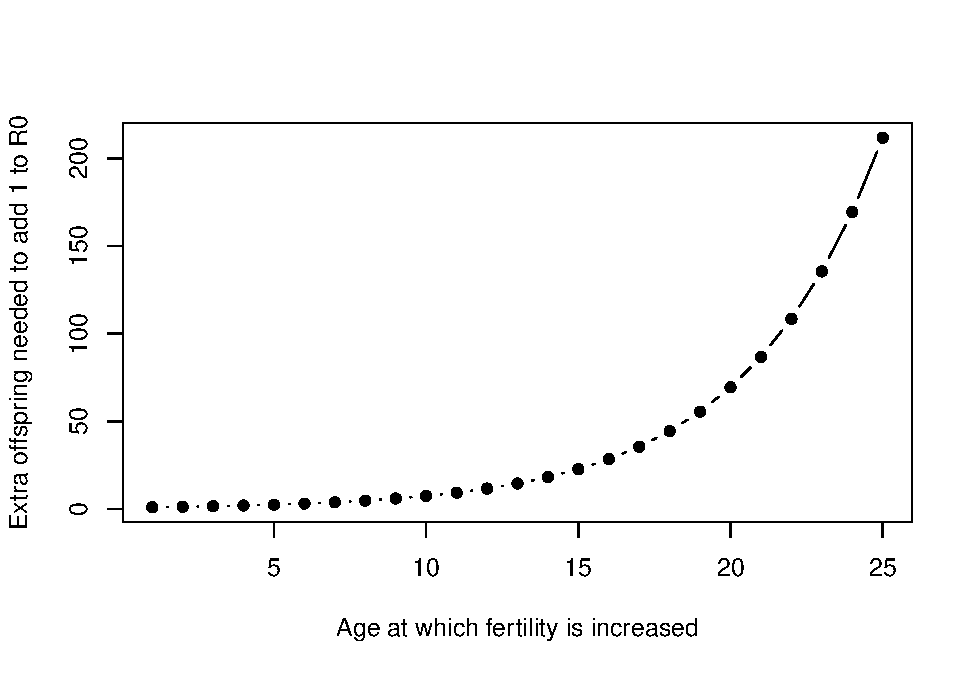
\includegraphics[keepaspectratio,alt={\label{fig:forceselectionplot}Extra offspring needed at each age to raise R0 by 1, when annual survival is 0.8.}]{BB512_files/BB512_files/figure-latex/forceselectionplot-1.pdf}}
\caption{\label{fig:forceselectionplot}Extra offspring needed at each age to raise R0 by 1, when annual survival is 0.8.}
\end{figure}

\emph{Reset everything again (mx =10; survival = 0.8). Set mx from age 15 onwards to be 0. Now alter survival rate after this point (at ages 15-25). What happens to fitness?}

You should notice that any changes you make to survival AFTER reproduction has been completed will have no effect on fitness. In other words evolution ``doesn't care about you'' after you have finished with reproduction.

This is only true for an individual's \emph{own} offspring. If older individuals help their relatives to survive and reproduce, survival after reproduction can still raise their inclusive fitness: see the grandmother hypothesis and killer whales in the lecture.

\emph{Questions}

\begin{itemize}
\tightlist
\item
  \emph{The declining force of selection.} A change in survival or reproduction at age \(x\) only affects the individuals still alive at that age, so its effect on fitness shrinks as survivorship (\(l_x\)) falls and as less of the lifetime's reproduction remains. Selection therefore acts strongly on early life and weakly on late life. Early reproduction, and genes with early benefits and late costs, are favoured, and senescence can evolve.
\item
  \emph{Age-related disease in humans.} Many diseases of old age (e.g.~many cancers, heart disease, dementia) have their main effects after most reproduction has happened, so selection against them is weak. Harmful mutations with late effects can build up (mutation accumulation), and some genes that cause late disease may have been favoured for their early benefits (antagonistic pleiotropy).
\item
  \emph{Predation risk.} Where predation is high, an individual is unlikely to survive to old age whatever it invests in its body, so resources spent on maintenance and repair are less valuable. Selection should favour putting more into early reproduction and less into maintenance.
\item
  \emph{Survival after reproduction.} Older individuals can raise inclusive fitness by helping relatives. Post-reproductive killer whale females lead their groups to salmon when food is scarce, and in humans, grandmothers can improve their grandchildren's survival (the grandmother hypothesis).
\end{itemize}

\section{Solutions: Hardy-Weinberg equilibrium}\label{solutions-hardy-weinberg-equilibrium}

Answers to the Hardy-Weinberg questions.

Remember the basic formulas:
\(p^2 + 2pq + q^2 = 1\) and \(p + q = 1\)

\(p\) = frequency of allele A (the dominant allele in these problems)

\(q\) = frequency of allele a (the recessive allele)

\(p^2\) = frequency of homozygous AA individuals

\(q^2\) = frequency of homozygous aa individuals

\(2pq\) = frequency of heterozygous Aa individuals

\subsection{Problem 1}\label{problem-1}

The frequency of allele \emph{a}: Since \(p + q = 1\) and \(p = 0.7\), \(q = 1 - 0.7 = 0.3\).

The expected genotype frequencies:

\begin{itemize}
\tightlist
\item
  \emph{AA} = \(p^2 = 0.7 \times 0.7 = 0.49\) (49\%)
\item
  \emph{Aa} = \(2pq = 2 \times 0.7 \times 0.3 = 0.42\) (42\%)
\item
  \emph{aa} = \(q^2 = 0.3 \times 0.3 = 0.09\) (9\%)
\end{itemize}

Check: \(0.49 + 0.42 + 0.09 = 1\).

The phenotype frequencies if \emph{A} is completely dominant over \emph{a}: Both \emph{AA} and \emph{Aa} individuals show the dominant phenotype, so its frequency is \(0.49 + 0.42 = 0.91\) (91\%). Only \emph{aa} individuals show the recessive phenotype, so its frequency is 0.09 (9\%). Notice that the heterozygotes cannot be told apart from the \emph{AA} homozygotes by looking at them.

\subsection{Problem 2}\label{problem-2}

9\% = 0.09 = HbS/HbS = \(q^2\). To find \(q\), take the square root of 0.09 to get 0.3. Since \(p = 1 - 0.3\), \(p\) must equal 0.7. \(2pq = 2 \times 0.7 \times 0.3 = 0.42\), so 42\% of babies are expected to be heterozygous (HbA/HbS) at birth.

Among adults this figure would usually be higher, and the HbS/HbS frequency lower, because heterozygotes survive better than either homozygote. That is selection acting on the genotypes after birth, which is why we applied HWE at birth.

\subsection{Problem 3}\label{problem-3}

The allele frequencies: 200 diploid individuals carry 400 allele copies. Each \emph{AA} individual carries two copies of \emph{A} and each \emph{Aa} individual carries one, so the number of \emph{A} copies is \(2 \times 120 + 40 = 280\).

\(p = 280 / 400 = 0.7\), and \(q = 1 - 0.7 = 0.3\). (Check: the number of \emph{a} copies is \(2 \times 40 + 40 = 120\), and \(120 / 400 = 0.3\).)

The expected counts under HWE are the expected frequencies multiplied by the sample size, 200:

{\def\LTcaptype{none} % do not increment counter
\begin{longtable}[]{@{}lll@{}}
\toprule\noalign{}
Genotype & Observed & Expected under HWE \\
\midrule\noalign{}
\endhead
\bottomrule\noalign{}
\endlastfoot
\emph{AA} & 120 & \(0.49 \times 200 = 98\) \\
\emph{Aa} & 40 & \(0.42 \times 200 = 84\) \\
\emph{aa} & 40 & \(0.09 \times 200 = 18\) \\
\end{longtable}
}

Comparison: there are far fewer heterozygotes than expected (40 observed against 84 expected), and more of both homozygotes than expected. This is a heterozygote deficit.

Possible explanations include inbreeding or other non-random mating, the sample combining two or more partly separated subpopulations (the Wahlund effect), selection against heterozygotes, or genotyping errors (for example, heterozygotes being misread as homozygotes). With a deficit this large it is unlikely to be chance alone, but a formal statistical test would be needed to confirm that. The comparison tells us there is a pattern to investigate, not which of these causes is responsible.

\subsection{Problem 4}\label{problem-4}

The first thing you'll need to do is obtain \(p\) and \(q\). So, since white is recessive (i.e.~\emph{bb}), and 40\% of the butterflies are white, then \emph{bb} = \(q^2\) = 0.4.
To determine \(q\), which is the frequency of the recessive allele in the population, take the square root of \(q^2\) which is 0.632. So, \(q = 0.63\). Since \(p + q = 1\), then \(p\) must be \(1 - 0.63 = 0.37\).

Now then, to answer our questions. First, what is the percentage of butterflies in the population that are heterozygous? Well, that would be \(2pq\) so the answer is \(2 \times 0.37\times 0.63 = 0.47\). Second, what is the frequency of homozygous dominant individuals? That would be \(p^2\) or \(0.37^2 = 0.14\).

\emph{Extension:} Brown butterflies are those with genotype \emph{BB} or \emph{Bb}, so they make up \(1 - 0.4 = 0.6\) of the population (check: \(0.14 + 0.47 \approx 0.6\)). Of these, the heterozygotes are \(0.47 / 0.60 \approx 0.78\), so about 78\% of brown butterflies are expected to be heterozygous. Note the difference between this and the 47\% heterozygotes in the population as a whole: here the denominator is only the brown butterflies.

\section{Solutions: Gene pool model}\label{solutions-gene-pool-model}

\subsection{Part 2: Drift through time}\label{part-2-drift-through-time}

\begin{enumerate}
\def\labelenumi{\arabic{enumi}.}
\tightlist
\item
  \textbf{How does population size affect the variation through time in allele frequencies? Why do you see these patterns?}

  \begin{itemize}
  \tightlist
  \item
    Each generation is a random sample of 2N alleles from the previous gene pool. The smaller the sample, the larger the sampling error, so allele frequencies fluctuate much more in small populations. With N = 20 the frequency of \emph{A} wanders widely and usually hits 0 or 1 within 100 generations; with N = 1000 it stays close to 0.5 over the same period.
  \end{itemize}
\item
  \textbf{With 20 individuals, does \emph{A} always end up fixed, or is it sometimes lost?}

  \begin{itemize}
  \tightlist
  \item
    Both happen, roughly equally often. Drift has no direction: starting from 0.5, \emph{A} is fixed in about half of the populations and lost in the other half.
  \end{itemize}
\item
  \textbf{When the population size is large (say 1000), can you see an allele become fixed within 100 generations? Could it happen if you ran the simulation for much longer?}

  \begin{itemize}
  \tightlist
  \item
    Not within 100 generations: in large populations drift is slow. But yes, given enough time an allele is eventually fixed even in a large population. Starting from p = 0.5, the expected time until one allele is fixed is about \(2.8N\) generations (more precisely \(-4N[p \ln p + q \ln q]\)), i.e.~around 55 generations for N = 20 and around 2,800 generations for N = 1000. With \texttt{n\_gen\ \textless{}-\ 3000} you will see fixation in some runs but not all.
  \end{itemize}
\end{enumerate}

\subsection{Part 3: Many populations}\label{part-3-many-populations-1}

\begin{enumerate}
\def\labelenumi{\arabic{enumi}.}
\tightlist
\item
  \textbf{What proportion of the populations have lost one of their alleles by generation 100 for N = 20, 100 and 1000?}

  \begin{itemize}
  \tightlist
  \item
    Roughly 90\% for N = 20, around 10 to 15\% for N = 100, and essentially none for N = 1000 (exact numbers will vary between runs).
  \end{itemize}
\item
  \textbf{Of the populations where one allele was fixed, in what proportion was it \emph{A}? Does this depend on population size?}

  \begin{itemize}
  \tightlist
  \item
    About half, at every population size. Starting from a frequency of 0.5, \emph{A} and \emph{a} have equal chances of being fixed.
  \end{itemize}
\item
  \textbf{So what does population size change: which allele is fixed, or how quickly variation is lost?}

  \begin{itemize}
  \tightlist
  \item
    How quickly. For a neutral allele, the probability of fixation equals its starting frequency whatever the population size. Population size determines the \emph{speed} of drift: small populations lose variation quickly, large populations slowly.
  \end{itemize}
\item
  \textbf{Are rare alleles more or less likely to be lost than common ones?}

  \begin{itemize}
  \tightlist
  \item
    More likely. A neutral allele at frequency \(p\) is eventually fixed with probability \(p\) and lost with probability \(1 - p\). So an allele at 0.1 is lost 90\% of the time, and an allele at 0.75 is lost only 25\% of the time.
  \end{itemize}
\item
  \textbf{Compare the proportion of populations where the new allele was fixed with \(1/(2N)\). What does this tell you about the fate of most new mutations?}

  \begin{itemize}
  \tightlist
  \item
    With N = 20, a single new copy starts at \(1/40 = 0.025\), and roughly 2 to 3\% of populations end up fixed for it (with 200 replicates you might see anywhere from about 1\% to 5\%). This matches \(1/(2N)\). Most new neutral mutations, about 39 out of 40 here and 1,999 out of 2,000 in a population of 1000, are lost by chance, usually within a few generations. This is the ``Model 1'' result from the lecture.
  \end{itemize}
\item
  \textbf{Can you find a simple rule linking starting frequency to probability of fixation?}

  \begin{itemize}
  \tightlist
  \item
    The probability of fixation of a neutral allele equals its starting frequency.
  \end{itemize}
\item
  \textbf{Going further: does the simulated decline in \(H_e\) agree with \(H_t = H_0 (1 - 1/(2N))^t\)?}

  \begin{itemize}
  \tightlist
  \item
    Yes. Averaged over many populations, \(H_e\) declines smoothly and follows the theoretical curve closely (with N = 20, it falls by about 2.5\% per generation, from 0.5 to about 0.04 after 100 generations). Individual populations are noisy, which is why the average is needed. Note that \(H_e\) declines in every case, even though the average allele frequency across populations stays at about 0.5: drift removes variation \emph{within} populations while creating differences \emph{between} them.
  \end{itemize}
\end{enumerate}

\subsection{Part 4: Bottlenecks and founder effects}\label{part-4-bottlenecks-and-founder-effects-1}

\begin{enumerate}
\def\labelenumi{\arabic{enumi}.}
\tightlist
\item
  \textbf{How does a genetic bottleneck influence the genetic composition of the population?}

  \begin{itemize}
  \tightlist
  \item
    During the bottleneck the population is small, so drift is strong and allele frequencies can change a lot in a few generations. One allele may be lost altogether. The genetic composition after the bottleneck is therefore often quite different from that before it, and genetic diversity is usually reduced.
  \end{itemize}
\item
  \textbf{How might a genetic bottleneck affect the probability that one allele is fixed and the other lost?}

  \begin{itemize}
  \tightlist
  \item
    It greatly increases it. With 10 individuals for about 20 generations, roughly half of all runs lose one allele during the bottleneck, whereas in a constant population of 1000 this essentially never happens within 100 generations. Which allele is fixed is still a matter of chance.
  \end{itemize}
\item
  \textbf{What happens to allele frequency after the bottleneck? Does the population ``recover'' its original allele frequency?}

  \begin{itemize}
  \tightlist
  \item
    No.~Once the population is large again, drift is weak, so the frequency stays close to wherever the bottleneck left it. Nothing pulls it back to 0.5. If an allele was lost, it cannot return without mutation or migration. The effects of a bottleneck persist long after the population has recovered in size.
  \end{itemize}
\item
  \textbf{Does the severity of the bottleneck (i.e.~length and population size) matter?}

  \begin{itemize}
  \tightlist
  \item
    Yes. Smaller and longer bottlenecks cause larger changes and a higher chance of losing an allele. Each generation of the bottleneck multiplies heterozygosity by \(1 - 1/(2N)\), so 20 generations at N = 10 leaves about \((1 - 1/20)^{20} \approx 0.36\) of the original heterozygosity, whereas 20 generations at N = 100 leaves about 0.90.
  \end{itemize}
\item
  \textbf{Founder effects: how different are the new populations from the source population, and from each other? How would this change with 50 founders?}

  \begin{itemize}
  \tightlist
  \item
    Although the source population has a frequency of 0.5, the founded populations typically range from about 0.3 to 0.7, and some are further off. They also differ from each other. The spread reflects sampling only 20 alleles (standard deviation about \(\sqrt{0.5 \times 0.5 / 20} \approx 0.11\)). With 50 founders (100 alleles), the spread is smaller (standard deviation about 0.05), so the new populations resemble the source population more closely.
  \end{itemize}
\end{enumerate}

\subsection{Conclusions}\label{conclusions-1}

\begin{enumerate}
\def\labelenumi{\arabic{enumi}.}
\tightlist
\item
  \textbf{What are the limitations of this simulation?}

  \begin{itemize}
  \tightlist
  \item
    The model makes the assumptions listed at the start, and each is a limitation:

    \begin{itemize}
    \tightlist
    \item
      \textbf{No selection:} in reality, some alleles affect survival or reproduction.
    \item
      \textbf{No mutation:} new alleles never arise, so variation can only be lost. In real populations, mutation replenishes variation (mutation-drift balance).
    \item
      \textbf{No migration:} real populations exchange genes, which can restore lost alleles and counteract drift.
    \item
      \textbf{Random mating:} real populations may show inbreeding or assortative mating.
    \item
      \textbf{Constant population size and non-overlapping generations:} real populations fluctuate in size and have overlapping generations, and not all individuals breed. The relevant population size for drift (the \emph{effective} population size) is usually much smaller than the census size.
    \item
      \textbf{One locus with two alleles:} real genomes have many loci, many with more than two alleles, and linked loci are not independent.
    \end{itemize}
  \end{itemize}
\item
  \textbf{Why is genetic diversity important to a population, for example in a conservation context?}

  \begin{itemize}
  \tightlist
  \item
    Genetic diversity is crucial for the adaptability and survival of a population. In a conservation context:

    \begin{itemize}
    \tightlist
    \item
      \textbf{Resilience to diseases:} a genetically diverse population is less likely to be wiped out by a single disease, as some individuals might have resistance.
    \item
      \textbf{Adaptation to changing environments:} diversity provides the variation that selection needs if conditions change.
    \item
      \textbf{Reduced inbreeding:} high genetic diversity reduces the chance that individuals inherit two copies of harmful recessive alleles, which lowers fitness (inbreeding depression).
    \item
      \textbf{Long-term survival:} small populations lose diversity through drift, which is why conservation programmes try to keep populations large and connected.
    \end{itemize}
  \end{itemize}
\item
  \textbf{Can you think of real-life scenarios where understanding gene pool dynamics would be valuable?}

  \begin{itemize}
  \tightlist
  \item
    \textbf{Conservation biology:} managing captive breeding and reintroductions to retain genetic diversity, or moving individuals between isolated populations (``genetic rescue'').
  \item
    \textbf{Medical genetics:} founder effects explain why some genetic disorders are unusually common in particular populations descended from small founding groups.
  \item
    \textbf{Agriculture:} maintaining diversity in crop and livestock breeding programmes.
  \end{itemize}
\item
  \textbf{Challenge: how could you simulate a population that is steadily shrinking through time?}

  \begin{itemize}
  \tightlist
  \item
    Inside the loop, set the population size as a function of the generation number before sampling, for example \texttt{pop\_size\ \textless{}-\ round(1000\ *\ 0.95\^{}(i\ -\ 1))} for a 5\% decline per generation, or \texttt{pop\_size\ \textless{}-\ max(10,\ 1000\ -\ 10\ *\ i)} for a linear decline to a floor of 10. As the population shrinks, drift becomes stronger and the frequency of \emph{A} fluctuates more and more until one allele is fixed.
  \end{itemize}
\end{enumerate}

\section{Solutions: Neutral or adaptive evolution in humans}\label{solutions-neutral-or-adaptive-evolution-in-humans}

There is no single correct ordering: groups can defend different placements. What matters is the reasoning. A good answer for each trait goes through three questions:

\begin{enumerate}
\def\labelenumi{\arabic{enumi}.}
\tightlist
\item
  \textbf{Is the variation heritable?} If not, the trait cannot evolve by drift \emph{or} by selection.
\item
  \textbf{How strongly does the trait affect survival or reproduction, in this environment?} Strong effects put the trait at the selection end of the continuum; weak or no effects put it at the drift end.
\item
  \textbf{Is the population large enough for that selection to beat drift?} Selection is effective only when \(s\) is clearly larger than about \(1/(2N_e)\).
\end{enumerate}

The take-home message is that whether a trait evolves adaptively or neutrally depends on the environment (and on population size), not just on the trait. A useful comparison is antibiotic resistance in bacteria. With antibiotics, resistance genes are strongly selected \emph{for}. Without antibiotics they are not neutral: resistance usually has a fitness cost, so it is usually selected \emph{against} (which is why resistance can decline when an antibiotic is used less, although compensatory mutations can reduce the cost). The environment can change both the strength and the direction of selection.

Humans are still evolving. In industrialised societies such as Denmark, almost everyone survives to adulthood, so selection now acts mainly through differences in the number of children people have (and the age at which they have them), rather than through survival. Studies of modern populations have measured selection on traits such as height, age at first birth and cholesterol in exactly this way (e.g.~Byars et al.~2010, \emph{PNAS}; Sanjak et al.~2018, \emph{PNAS}).

\subsection{Suggested placements}\label{suggested-placements}

{\def\LTcaptype{none} % do not increment counter
\begin{longtable}[]{@{}
  >{\raggedright\arraybackslash}p{(\linewidth - 8\tabcolsep) * \real{0.2000}}
  >{\raggedright\arraybackslash}p{(\linewidth - 8\tabcolsep) * \real{0.2000}}
  >{\raggedright\arraybackslash}p{(\linewidth - 8\tabcolsep) * \real{0.2000}}
  >{\raggedright\arraybackslash}p{(\linewidth - 8\tabcolsep) * \real{0.2000}}
  >{\raggedright\arraybackslash}p{(\linewidth - 8\tabcolsep) * \real{0.2000}}@{}}
\toprule\noalign{}
\begin{minipage}[b]{\linewidth}\raggedright
Trait
\end{minipage} & \begin{minipage}[b]{\linewidth}\raggedright
Heritable variation?
\end{minipage} & \begin{minipage}[b]{\linewidth}\raggedright
As foragers
\end{minipage} & \begin{minipage}[b]{\linewidth}\raggedright
In Denmark today
\end{minipage} & \begin{minipage}[b]{\linewidth}\raggedright
Where on the drift-selection continuum, and why
\end{minipage} \\
\midrule\noalign{}
\endhead
\bottomrule\noalign{}
\endlastfoot
Metabolic efficiency & Yes, partly & Probably important: food was often scarce, so efficient use of energy aided survival and reproduction & Weak, possibly reversed: food is abundant, and very efficient storage may contribute to obesity and type 2 diabetes & Towards selection as foragers; weaker today. \emph{Debatable}: the ``thrifty gene'' idea has weak direct genetic support \\
Amount of body hair & Yes & Probably weak (temperature regulation, parasites, mate choice are all suggested) & Weak, apart from possible mate choice & Probably near the drift end, with some selection (e.g.~sexual selection). \emph{Debatable} \\
Singing ability & Partly & Unknown; possibly sexual selection or social bonding & Weak & Near the drift end, but sexual selection is possible. \emph{Debatable} \\
Intelligence & Yes, within populations (variation among individuals) & Probably important for problem solving and social life & Unclear: in modern data, educational attainment is weakly associated with having \emph{fewer} children & Somewhere in the middle; the direction of selection may differ between environments. Within-population heritability says nothing about differences between groups (see the note in the practical) \\
Eye colour & Yes, strongly (mainly \emph{OCA2}/\emph{HERC2}) & Probably weak, except perhaps through mate choice & Weak & Blue eyes rose quickly in Europe, which suggests some selection (on pigmentation in general, or sexual selection), but drift and ``hitch-hiking'' with selected pigmentation alleles are possible. \emph{Debatable} \\
Earwax type (\emph{ABCC11}) & Yes, simple (one DNA change) & Unknown; a selection signal exists, perhaps linked to sweat or body odour & Weak & Some evidence of past selection, target uncertain (see evidence card). \emph{Debatable} \\
Sperm motility & Partly & Strong: affects fertilisation directly & Still selected, but assisted reproduction reduces selection for some couples & Towards selection: tightly linked to reproduction \\
Muscle strength & Partly & Probably important for hunting, carrying and fighting & Weak & Towards selection as foragers; nearer the drift end today \\
Face symmetry & Weakly; much is developmental noise & Possibly via mate choice, as a cue of health & Weak & Mostly not heritable, so it can evolve little by either process \\
Running speed & Partly & Probably important for hunting and escaping danger & Weak & Towards selection as foragers; nearer the drift end today \\
Height & Yes, highly heritable (many genes) & Probably selected, but the optimum depends on environment & Modern studies detect weak selection, mainly through number of children, with differences between the sexes (e.g.~Stulp et al.~2015, \emph{Proc. R. Soc. B}) & In the middle: weak but measurable selection \\
Birth canal (pelvic) shape & Yes & Stabilising selection: the canal must allow birth of a big-brained baby while still allowing efficient walking & Weaker: caesarean section reduces the cost of a mismatch & Selection keeps the shape within limits, but much of the variation between populations fits drift during serial founder effects as humans spread out of Africa (Betti \& Manica 2018, \emph{Proc. R. Soc. B}; see the drift lecture). A good example of both acting together \\
Resistance to bubonic plague & Yes, partly (immune genes) & Weak: plague is a disease of dense agricultural and urban societies, not of small foraging groups & Weak: plague is rare and treatable & Strongly selected in medieval Europe during the Black Death (Klunk et al.~2022, \emph{Nature}, immune genes such as \emph{ERAP2}), not in foragers and not today. A clear example of environment-dependent selection \\
Sense of smell & Yes (hundreds of olfactory receptor genes) & Probably important for finding food and avoiding danger & Weak & Many human olfactory receptor genes have become non-functional, which is consistent with relaxed selection followed by drift. Near the drift end today \\
Resistance to common cold & Partly & Weak: rarely fatal & Weak & Near the drift end: colds rarely affect survival or number of children \\
Eyesight acuity & Partly & Probably important for hunting and gathering & Weak: glasses correct poor vision & Towards selection as foragers; near the drift end today \\
\end{longtable}
}

Examples of traits that \textbf{cannot} evolve much because their variation is mostly not heritable: the fine texture of the iris, the detailed ridge minutiae of fingerprints (these differ between identical twins), and much of the variation in face symmetry.

\subsection{Gene flow between populations}\label{gene-flow-between-populations}

\begin{itemize}
\tightlist
\item
  Differences that gene flow would erase: neutral variation (most DNA differences, and traits close to the drift end of the continuum). Very few migrants per generation are enough to prevent large neutral differences between populations, which is one reason why most human genetic variation is found \emph{within} populations rather than between them.
\item
  Differences that local selection can maintain against gene flow: traits where the selection coefficient is large compared with the migration rate. Examples are skin pigmentation (UV intensity differs with latitude), lactase persistence (dairying history), and HbS and Duffy-null (malaria). These traits vary between populations much more than most neutral markers do.
\end{itemize}

\subsection{Discussion questions}\label{discussion-questions}

\begin{itemize}
\tightlist
\item
  \textbf{Traits categorised differently between the two societies.} Muscle strength, running speed, eyesight acuity and metabolic efficiency were probably more strongly selected in foraging societies than in Denmark today. Others (e.g.~plague resistance) were strongly selected only in particular historical environments. In both settings, though, selection still acts, especially through the number of children.
\item
  \textbf{Traits with little heritable variation.} Iris texture, fingerprint detail and much of face symmetry: they can vary a lot but cannot evolve much by either process.
\item
  \textbf{Gene flow vs local selection.} See above.
\item
  \textbf{Preconceived notions.} Common ones are that ``evolution has stopped in humans'' (it has not), that ``every trait is an adaptation'' (many traits drift, and some barely vary heritably), and that ``drift only matters in tiny populations'' (it acts in every finite population; it dominates whenever \(s\) is small compared with \(1/(2N_e)\)).
\item
  \textbf{Other traits to add.} Lactase persistence, skin pigmentation, blood groups, alcohol flush reaction, ability to taste bitter compounds (\emph{TAS2R38}), and wisdom teeth are all good candidates with some genetic evidence.
\end{itemize}

\section{Solutions: Heritability}\label{solutions-heritability}

\emph{Predictions.} If offspring were on average exactly like their parents, the slope would be 1 (\(h^2 = 1\)). If offspring were no more like their own parents than like any other bird, the line would be flat (slope 0, \(h^2 = 0\)). A slope in between means that offspring resemble their parents partly: on average, they lie part of the way between their parents' value and the population mean (``regression towards the mean'').

After downloading the file, you can read in the data like this (or use the ``Import Dataset'' wizard in RStudio):

\begin{Shaded}
\begin{Highlighting}[]
\NormalTok{pop\_1 }\OtherTok{\textless{}{-}} \FunctionTok{read.csv}\NormalTok{(}\StringTok{"data/Heritability\_Pop1.csv"}\NormalTok{)}
\end{Highlighting}
\end{Shaded}

Plot the data and fit the model as follows.

\begin{Shaded}
\begin{Highlighting}[]
\CommentTok{\# Plot the relationship}
\FunctionTok{plot}\NormalTok{(pop\_1}\SpecialCharTok{$}\NormalTok{Midparent\_value, pop\_1}\SpecialCharTok{$}\NormalTok{Offspring\_value,}
     \AttributeTok{xlab =} \StringTok{"Mid{-}parent wing length (mm)"}\NormalTok{,}
     \AttributeTok{ylab =} \StringTok{"Offspring wing length (mm)"}\NormalTok{)}

\CommentTok{\# Fit the linear regression model}
\NormalTok{mod1 }\OtherTok{\textless{}{-}} \FunctionTok{lm}\NormalTok{(Offspring\_value }\SpecialCharTok{\textasciitilde{}}\NormalTok{ Midparent\_value, }\AttributeTok{data =}\NormalTok{ pop\_1)}

\CommentTok{\# Add the regression line to the plot}
\FunctionTok{abline}\NormalTok{(mod1, }\AttributeTok{col =} \StringTok{"red"}\NormalTok{)}
\end{Highlighting}
\end{Shaded}

\pandocbounded{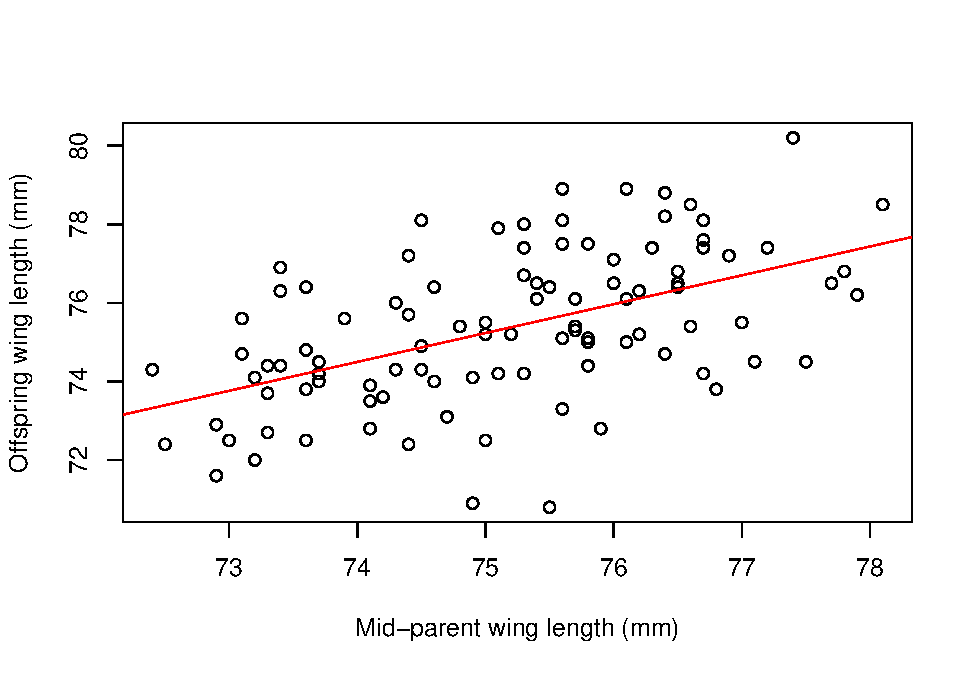
\includegraphics[keepaspectratio]{BB512_files/BB512_files/figure-latex/plotheritability-1.pdf}}

\begin{Shaded}
\begin{Highlighting}[]
\CommentTok{\# Summarise the model, and get the 95\% confidence interval of the slope}
\FunctionTok{summary}\NormalTok{(mod1)}
\end{Highlighting}
\end{Shaded}

\begin{verbatim}
## 
## Call:
## lm(formula = Offspring_value ~ Midparent_value, data = pop_1)
## 
## Residuals:
##     Min      1Q  Median      3Q     Max 
## -4.7982 -1.0608  0.0486  1.1242  3.2360 
## 
## Coefficients:
##                 Estimate Std. Error t value Pr(>|t|)    
## (Intercept)      20.1633     9.1736   2.198   0.0303 *  
## Midparent_value   0.7342     0.1220   6.018 3.06e-08 ***
## ---
## Signif. codes:  0 '***' 0.001 '**' 0.01 '*' 0.05 '.' 0.1 ' ' 1
## 
## Residual standard error: 1.663 on 98 degrees of freedom
## Multiple R-squared:  0.2699, Adjusted R-squared:  0.2624 
## F-statistic: 36.22 on 1 and 98 DF,  p-value: 3.059e-08
\end{verbatim}

\begin{Shaded}
\begin{Highlighting}[]
\FunctionTok{confint}\NormalTok{(mod1)[}\DecValTok{2}\NormalTok{, ]}
\end{Highlighting}
\end{Shaded}

\begin{verbatim}
##     2.5 %    97.5 % 
## 0.4921315 0.9763443
\end{verbatim}

\emph{What is your estimate of \(h^2\), and how precise is it?}

The heritability is the slope of the relationship: 0.73, with a 95\% confidence interval of 0.49 to 0.98. This is a high heritability. (The data were simulated with a true value of 0.70.)

\emph{What does this heritability tell us about the variation in wing length in this population? What does it not tell us about any one bird?}

About 73\% of the variation in wing length among birds in this population is due to additive genetic differences between them. It does not mean that 73\% of any one bird's wing length ``comes from its genes'': heritability describes variation in a population, not individuals. It also applies only to this population in this environment.

\emph{What else might explain the remaining variation?}

The remaining 27\% or so is due to differences in the environment that the birds grew up in (for example food supply, brood size, weather during the nestling period, parasites), to chance events during development, to measurement error, and to any non-additive genetic effects (dominance and interactions between genes).

\emph{Calculate \(V_P\) and \(V_A\).}

\begin{Shaded}
\begin{Highlighting}[]
\NormalTok{VP\_1 }\OtherTok{\textless{}{-}} \FunctionTok{var}\NormalTok{(pop\_1}\SpecialCharTok{$}\NormalTok{Offspring\_value)}
\NormalTok{VA\_1 }\OtherTok{\textless{}{-}} \FunctionTok{coef}\NormalTok{(mod1)[}\DecValTok{2}\NormalTok{] }\SpecialCharTok{*}\NormalTok{ VP\_1}
\NormalTok{VP\_1}
\end{Highlighting}
\end{Shaded}

\begin{verbatim}
## [1] 3.7496
\end{verbatim}

\begin{Shaded}
\begin{Highlighting}[]
\NormalTok{VA\_1}
\end{Highlighting}
\end{Shaded}

\begin{verbatim}
## Midparent_value 
##        2.753098
\end{verbatim}

\(V_P\) = 3.75 mm² and \(V_A = h^2 \times V_P\) = 0.73 × 3.75 = 2.75 mm². We use the offspring values for \(V_P\) because each offspring value is a single bird's phenotype. Each mid-parent value is the mean of two birds, and averaging two independent values halves the variance, so \texttt{var(pop\_1\$Midparent\_value)} (here 1.88 mm²) is only about half of \(V_P\).

\emph{Predict the response to selection with \(S\) = 2 mm.}

\(R = h^2 S\) = 0.73 × 2 = 1.47 mm: the mean wing length of the next generation should increase by about 1.5 mm.

The graph for the second population looks like this:

\begin{Shaded}
\begin{Highlighting}[]
\NormalTok{pop\_2 }\OtherTok{\textless{}{-}} \FunctionTok{read.csv}\NormalTok{(}\FunctionTok{file.path}\NormalTok{(pathToDirectory, }\StringTok{"heritability\_pop2.csv"}\NormalTok{))}
\FunctionTok{plot}\NormalTok{(pop\_2}\SpecialCharTok{$}\NormalTok{Midparent\_value, pop\_2}\SpecialCharTok{$}\NormalTok{Offspring\_value,}
     \AttributeTok{xlab =} \StringTok{"Mid{-}parent wing length (mm)"}\NormalTok{,}
     \AttributeTok{ylab =} \StringTok{"Offspring wing length (mm)"}\NormalTok{)}

\NormalTok{mod2 }\OtherTok{\textless{}{-}} \FunctionTok{lm}\NormalTok{(Offspring\_value }\SpecialCharTok{\textasciitilde{}}\NormalTok{ Midparent\_value, }\AttributeTok{data =}\NormalTok{ pop\_2)}
\FunctionTok{abline}\NormalTok{(mod2, }\AttributeTok{col =} \StringTok{"red"}\NormalTok{)}
\end{Highlighting}
\end{Shaded}

\pandocbounded{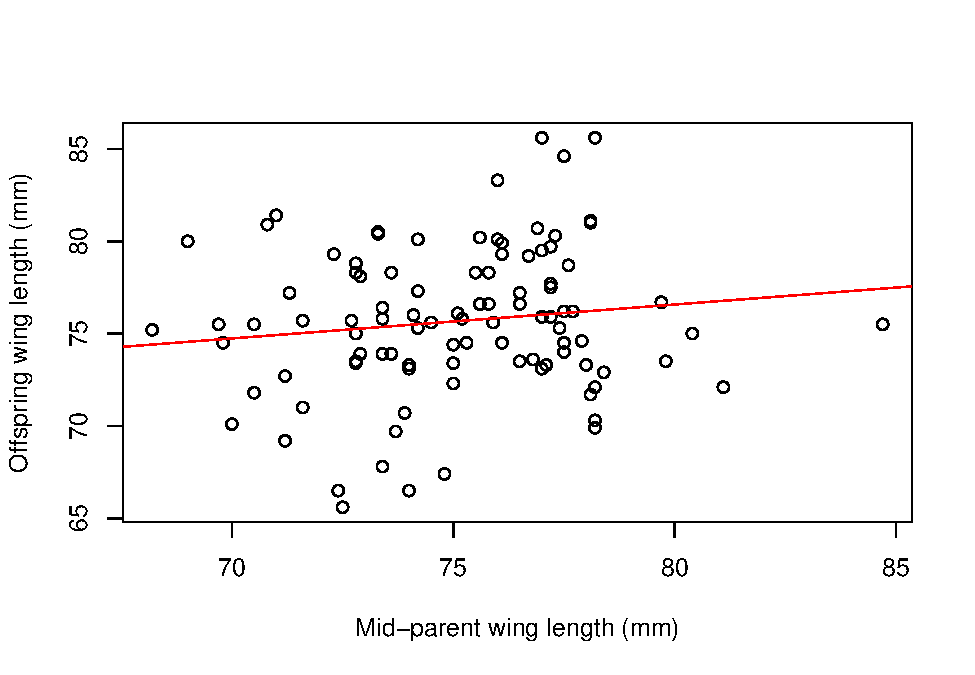
\includegraphics[keepaspectratio]{BB512_files/BB512_files/figure-latex/plotparentoffspring-1.pdf}}

\begin{Shaded}
\begin{Highlighting}[]
\FunctionTok{summary}\NormalTok{(mod2)}
\end{Highlighting}
\end{Shaded}

\begin{verbatim}
## 
## Call:
## lm(formula = Offspring_value ~ Midparent_value, data = pop_2)
## 
## Residuals:
##     Min      1Q  Median      3Q     Max 
## -9.5957 -2.3746  0.0433  2.8487  9.5781 
## 
## Coefficients:
##                 Estimate Std. Error t value Pr(>|t|)    
## (Intercept)      61.8846    10.4816   5.904 5.11e-08 ***
## Midparent_value   0.1836     0.1394   1.317    0.191    
## ---
## Signif. codes:  0 '***' 0.001 '**' 0.01 '*' 0.05 '.' 0.1 ' ' 1
## 
## Residual standard error: 3.969 on 98 degrees of freedom
## Multiple R-squared:  0.01738,    Adjusted R-squared:  0.007357 
## F-statistic: 1.734 on 1 and 98 DF,  p-value: 0.191
\end{verbatim}

\begin{Shaded}
\begin{Highlighting}[]
\FunctionTok{confint}\NormalTok{(mod2)[}\DecValTok{2}\NormalTok{, ]}
\end{Highlighting}
\end{Shaded}

\begin{verbatim}
##      2.5 %     97.5 % 
## -0.0931097  0.4603131
\end{verbatim}

\begin{Shaded}
\begin{Highlighting}[]
\NormalTok{VP\_2 }\OtherTok{\textless{}{-}} \FunctionTok{var}\NormalTok{(pop\_2}\SpecialCharTok{$}\NormalTok{Offspring\_value)}
\NormalTok{VA\_2 }\OtherTok{\textless{}{-}} \FunctionTok{coef}\NormalTok{(mod2)[}\DecValTok{2}\NormalTok{] }\SpecialCharTok{*}\NormalTok{ VP\_2}
\NormalTok{VP\_2}
\end{Highlighting}
\end{Shaded}

\begin{verbatim}
## [1] 15.8679
\end{verbatim}

\begin{Shaded}
\begin{Highlighting}[]
\NormalTok{VA\_2}
\end{Highlighting}
\end{Shaded}

\begin{verbatim}
## Midparent_value 
##        2.913374
\end{verbatim}

\emph{How does the heritability compare with population 1? Do the two confidence intervals overlap?}

For this population the heritability is 0.18 (95\% confidence interval -0.09 to 0.46), much lower than in population 1 (0.73). The two confidence intervals only just fail to overlap, and the interval for population 2 includes zero. (The true values used in the simulation were 0.18 and 0.70.) Note how wide both intervals are, even with 100 families: heritability is hard to estimate precisely, and estimates from a few dozen families are very uncertain. Report the uncertainty, not just the slope.

\emph{Compare \(V_P\) and \(V_A\) between the populations.}

{\def\LTcaptype{none} % do not increment counter
\begin{longtable}[]{@{}lll@{}}
\toprule\noalign{}
& Population 1 & Population 2 \\
\midrule\noalign{}
\endhead
\bottomrule\noalign{}
\endlastfoot
\(h^2\) & 0.73 & 0.18 \\
\(V_P\) (mm²) & 3.75 & 15.87 \\
\(V_A\) (mm²) & 2.75 & 2.91 \\
\(V_P - V_A\) (mm²) & 1.00 & 12.95 \\
\end{longtable}
}

The additive genetic variance is about the same in both populations (both data sets were simulated with \(V_A\) = 2.8 mm²). What differs is the phenotypic variance: population 2 is about four times as variable, and almost all of the extra variance is non-genetic. So heritability is lower in population 2 not because it has less genetic variation, but because its environment is more variable. This is why heritability is a property of a population in an environment, not of a trait.

\emph{Can you suggest environmental differences that could explain this?}

Anything that makes the conditions in which chicks grow up more variable in population 2 would do it. For example:

\begin{itemize}
\tightlist
\item
  \textbf{Food supply:} in a patchy habitat, some territories are rich and others poor, so chicks in different nests get very different amounts of food.
\item
  \textbf{Weather:} cold, wet spells during the nestling period reduce growth in some broods but not others, especially if breeding is spread over a long season.
\item
  \textbf{Brood size and competition:} chicks in large broods get less food each.
\item
  \textbf{Parasites and disease:} infection during growth reduces final size in some individuals.
\end{itemize}

In each case \(V_E\) increases, so \(V_P\) increases and \(h^2 = V_A/V_P\) falls, even though \(V_A\) is unchanged.

\emph{For the same selection differential, which population would respond faster to selection?}

Population 1. With \(S\) = 2 mm, \(R\) = 0.73 × 2 = 1.47 mm in population 1 but only 0.18 × 2 = 0.37 mm in population 2. In population 2, most of the difference between the selected parents and the rest of the population is environmental, and is not passed on.

\emph{Can you think of any real-world applications where understanding heritability would be important?}

\begin{itemize}
\tightlist
\item
  Agriculture: plant and animal breeding programmes use heritability to predict how fast yield, disease resistance or growth rate will respond to selection.
\item
  Conservation biology: the heritability of traits linked to survival and reproduction (for example breeding time, or tolerance of heat) indicates how fast a population might adapt to environmental change.
\item
  Fisheries and hunting: harvesting the largest individuals is a form of selection; heritability predicts how fast body size or age at maturity will evolve in response (compare the bighorn sheep example from the lecture).
\item
  Medicine: heritability estimates indicate how much of the variation in a disease risk is genetic, which guides the search for the genes involved (but a heritable condition can still be prevented or treated by changing the environment).
\end{itemize}

\emph{Violation of assumptions}

\begin{itemize}
\tightlist
\item
  \textbf{Additive genetic effects:} dominance and interactions between genes are not passed on predictably, so the slope estimates only the additive part; genotype-by-environment interactions mean that the estimate applies only to the environment studied.
\item
  \textbf{No shared environment:} if parents and offspring share a good or a poor territory, they resemble each other for non-genetic reasons, and \(h^2\) is overestimated. Cross-fostering removes this bias.
\item
  \textbf{Correct parentage:} extra-pair paternity means that some chicks are not the offspring of their social father, which weakens the resemblance and underestimates \(h^2\).
\item
  \textbf{Linearity:} if the relationship is curved (for example because of dominance, or because extreme parents produce offspring that do poorly), a straight line is a poor summary.
\item
  \textbf{Measurement accuracy:} errors in measuring the parents make the slope shallower (heritability is underestimated); errors in the offspring add noise and widen the confidence interval.
\item
  \textbf{Random mating:} if birds choose mates of similar size (assortative mating), the mid-parent values vary more than under random mating, and the simple regression no longer estimates \(h^2\) exactly.
\item
  \textbf{Representative sample:} if only some birds are measured, for example only those that survived a harsh winter (selection on wing length), the sample is biased.
\item
  \textbf{Independence:} if the same parent appears in several families, or several chicks from one nest are entered as separate points, the data points are not independent and the confidence interval will be too narrow.
\end{itemize}

\section{Solutions: Lotka-Volterra competition}\label{solutions-lotka-volterra-competition}

You can find a completed Excel spreadsheet \href{https://www.dropbox.com/s/q1qoqxhnm82uugw/9.\%20LV\%20Competition.xlsx?dl=1}{here}.

The answers to the questions are \href{https://www.dropbox.com/s/oz2c10bmyf8t7s6/9.\%20Answers\%20to\%20questions.pdf?dl=1}{here}.

The general conditions are in Neal, \emph{Interspecific Competition} (Lotka-Volterra competition section). Note that in the textbook, \(\alpha_{12}\) is written as \(\alpha\) and \(\alpha_{21}\) is written as \(\beta\).

The simplest way to understand the four outcomes is to ask whether each species can invade when it is rare and the other species is at its carrying capacity:

\begin{itemize}
\tightlist
\item
  When species 2 is at \(K_2\), a rare species 1 experiences crowding equivalent to \(\alpha_{12} K_2\) of its own individuals. It can grow if this is less than its own carrying capacity: \(\alpha_{12} K_2 < K_1\), or \(\alpha_{12} < K_1/K_2\).
\item
  In the same way, a rare species 2 can grow when species 1 is at \(K_1\) if \(\alpha_{21} K_1 < K_2\), or \(\alpha_{21} < K_2/K_1\).
\end{itemize}

{\def\LTcaptype{none} % do not increment counter
\begin{longtable}[]{@{}
  >{\raggedright\arraybackslash}p{(\linewidth - 4\tabcolsep) * \real{0.3333}}
  >{\raggedright\arraybackslash}p{(\linewidth - 4\tabcolsep) * \real{0.3333}}
  >{\raggedright\arraybackslash}p{(\linewidth - 4\tabcolsep) * \real{0.3333}}@{}}
\toprule\noalign{}
\begin{minipage}[b]{\linewidth}\raggedright
Species 1 can invade?
\end{minipage} & \begin{minipage}[b]{\linewidth}\raggedright
Species 2 can invade?
\end{minipage} & \begin{minipage}[b]{\linewidth}\raggedright
Outcome (question)
\end{minipage} \\
\midrule\noalign{}
\endhead
\bottomrule\noalign{}
\endlastfoot
Yes & No & Species 1 excludes species 2 (Q1) \\
No & Yes & Species 2 excludes species 1 (Q2) \\
Yes & Yes & Stable coexistence (Q3) \\
No & No & Either species can win, depending on the starting densities (Q4) \\
\end{longtable}
}

In ecological terms, coexistence requires that each species limits its own growth more than it limits its competitor's, once you allow for differences in carrying capacity. If the two species have similar carrying capacities, this means \(\alpha_{12} < 1\) and \(\alpha_{21} < 1\): each individual competes more strongly with members of its own species than with the other species, for example because the two species partly use different resources (niche differences).

Note that comparing a coefficient with 1 is not enough when the carrying capacities differ. In the answer to Q1, species 1 wins even though \(\alpha_{12} = 1.25 > 1\), because its carrying capacity is three times larger (\(K_1 = 3000\), \(K_2 = 1000\)).

\section{Solutions: Lotka-Volterra predator-prey dynamics}\label{solutions-lotka-volterra-predator-prey-dynamics}

You can find a completed Excel spreadsheet \href{https://www.dropbox.com/s/wet7brtgxywdqi5/10.\%20Pred-PreyDynamics.xlsx?dl=1}{here}.

The answers to the questions are \href{https://www.dropbox.com/s/mt43nvqu7cjif69/10.\%20Answers\%20to\%20Pred-Prey\%20exercise.pdf?dl=1}{here}.

\section{Solutions: Continuous-time Lotka-Volterra predator-prey model in R}\label{solutions-continuous-time-lotka-volterra-predator-prey-model-in-r}

All numbers below come from the chapter code with the default parameters (\(R = 0.25\), \(a = 0.01\), \(f = 0.008\), \(q = 0.1\)), start \(V = 1000\), \(C = 20\), run to time 200, unless stated otherwise.

\textbf{1. Oscillations}

\begin{itemize}
\tightlist
\item
  Both populations cycle regularly and for ever. The prey peak first (at \(t \approx 13.7, 53.8, 93.9, \ldots\)) and the predators peak about a quarter of a cycle later (\(t \approx 22.4, 62.5, 102.6, \ldots\)). Prey increase while predators are scarce; predators then increase because food is plentiful; the larger predator population pushes the prey down; the predators then starve and decline, and the cycle repeats.
\item
  With prey on the x-axis the orbit runs \textbf{anticlockwise}. Below the prey isocline (\(C < R/a = 25\)) prey increase (move right); above it they decrease (move left). To the right of the predator isocline (\(V > q/(af) = 1250\)) predators increase (move up); to the left they decrease (move down). Following these arrows round the four regions gives right, up, left, down: anticlockwise.
\end{itemize}

\textbf{2. Neutral stability and starting numbers}

\begin{itemize}
\tightlist
\item
  Starting exactly at \(V = 1250\), \(C = 25\) nothing changes: this is the equilibrium. Starting just next to it (\(V = 1300\), \(C = 25\)) gives a very small cycle (prey 1201 to 1300, predators 24.4 to 25.6), which does not grow or shrink.
\item
  Further away, the cycles are bigger: from \(V = 2000\), \(C = 20\) the prey range is 632 to 2180; from \(V = 1000\), \(C = 40\) it is 475 to 2601 (predators 14 to 41). In every case the size of the cycle stays the same for the whole run: the oscillations neither grow nor die away. This is \textbf{neutral stability}: the model has no tendency to return to the equilibrium or to move away from it, so the size of the cycles is set entirely by where you start.
\item
  The period changes a little with the size of the cycle: about 39.7 time units for the tiny cycle, about 40 at the default start, about 40.5 to 41.5 for the larger ones. For small cycles the period is \(2\pi/\sqrt{Rq} = 2\pi/\sqrt{0.025} \approx 39.7\).
\end{itemize}

\textbf{3. Equilibrium and time-averages}

\begin{itemize}
\tightlist
\item
  \(V^* = q/(af) = 0.1/(0.01 \times 0.008) = 1250\) and \(C^* = R/a = 0.25/0.01 = 25\).
\item
  The populations never settle there, but \texttt{mean(output\_df\$V)} = 1250.6 and \texttt{mean(output\_df\$C)} = 25.01: the \textbf{averages over the cycles equal the equilibrium} (the small difference is because the run does not end at the end of a complete cycle).
\end{itemize}

\textbf{4. Moving the isoclines}

\begin{itemize}
\tightlist
\item
  Doubling \(R\) (to 0.5) raises the prey isocline to \(C = 50\) (more predators are needed to stop the prey growing). Doubling \(a\) (to 0.02) lowers the prey isocline to \(C = 12.5\) \emph{and} moves the predator isocline left to \(V = 625\). Doubling \(f\) (to 0.016) moves only the predator isocline, to \(V = 625\). Doubling \(q\) (to 0.2) moves the predator isocline right, to \(V = 2500\). Because the starting point (1000, 20) is now a different distance from the new equilibrium, the cycles also change size.
\item
  With \(R = 0.2\) and \(q = 0.12\) the equilibrium moves to \(V^* = 1500\), \(C^* = 20\). The run gives average prey 1511 and average predators 19.95. So killing both species \textbf{increases the average number of prey} and decreases the average number of predators. This is Volterra's principle: an indiscriminate mortality factor (pesticide, fishing) can benefit the prey because it hits their predators.
\end{itemize}

\textbf{5. Extinction and reality}

\begin{itemize}
\tightlist
\item
  From \(V = 1000\), \(C = 100\) the predators fall to about 2.0 and the prey to about 8. In the model neither population can ever reach exactly zero (the growth rates are proportional to population size, so the populations approach zero but never reach it). In a real population, a handful of individuals, or a fraction of one, means extinction, and chance events (demographic stochasticity) would make it very likely.
\item
  Unrealistic assumptions include: prey grow exponentially without predators (no carrying capacity); each predator eats in proportion to prey density without limit (no handling time or satiation, i.e.~a Type I functional response); predator death rate is constant; no time lags, no refuges, no other prey or predators; individuals meet at random; populations are large enough to treat as continuous. Prey carrying capacity, predator satiation, refuges, alternative prey, spatial structure and environmental noise will all change the cycles: some damp them, others destabilise them, so real cycles are rarely neutrally stable.
\end{itemize}

\section{Solutions: Discrete-time Lotka-Volterra predator-prey model in R}\label{solutions-discrete-time-lotka-volterra-predator-prey-model-in-r}

All numbers below come from the chapter code with the default parameters (\(R = 0.25\), \(a = 0.01\), \(f = 0.008\), \(q = 0.1\)), start \(V = 1000\), \(C = 20\) and \texttt{total\_time\ =\ 300}. The model is deterministic, so you should get exactly these numbers.

\begin{itemize}
\tightlist
\item
  \textbf{Default run (\(\Delta t = 1\)).} Instead of a closed loop, the phase plot spirals \textbf{outwards}: each cycle is a little larger than the one before. By the last cycle the prey reach about 16,000 and the predators about 230. The prey hit zero at \(t = 220\); after that the predators have nothing to eat and dwindle towards zero (about 0.05 by \(t = 300\)). The populations ``react one step too late'': the change over each step is calculated from the numbers at the start of the step, so the prey keep growing for a whole step after predators have become numerous enough to stop them, and so on round the cycle.
\item
  \textbf{Smaller time steps.} With \(\Delta t = 0.1\) the spiral still grows, but much more slowly: over 300 time units the prey stay between about 670 and 2120 and neither population goes extinct. With \(\Delta t = 0.01\) the orbit is almost closed (prey up to about 1850), very close to the continuous-time model (prey 812 to 1823). Small time steps are just a more accurate way of calculating the continuous model.
\item
  \textbf{Larger time step.} With \(\Delta t = 2\) the spiral grows faster and the prey hit zero earlier, at \(t = 142\).
\item
  \textbf{Which parameters control the spiral?} \(R\) and \(q\). Doubling \(R\) (to 0.5) brings the prey crash forward from \(t = 220\) to \(t = 64\); doubling \(q\) (to 0.2) brings it forward to \(t = 58\). Doubling \(a\) or \(f\) also changes the time of the crash from the default start (\(t = 175\) and \(t = 154\)), but only because the equilibrium moves and the start is then a different distance from it. If you start the same relative distance from the equilibrium (e.g.~at 80 \% of \(V^*\) and \(C^*\)), doubling \(a\) or \(f\) makes no difference (crash at \(t = 220\), as with the defaults), while doubling \(R\) (\(t = 79\)) or \(q\) (\(t = 132\)) still speeds it up.
\item
  \textbf{Why.} Near the equilibrium, each step multiplies the distance from the equilibrium by about \(\sqrt{1 + \Delta t^2 R q}\). With the defaults this is \(\sqrt{1 + 0.025} \approx 1.012\), about 1 \% growth per step. The factor contains \(R\), \(q\) and \(\Delta t\) but not \(a\) or \(f\), and it is always bigger than 1, so the discrete model always spirals out eventually; it gets closer to 1 (no growth, as in the continuous model) as \(\Delta t\) gets smaller.
\end{itemize}

\section{Solutions: Game theory: Hawks and doves}\label{solutions-game-theory-hawks-and-doves}

Your own class results will differ from year to year. A worked analysis of real class data (2022) is in the \hyperref[results-of-the-hawk-dove-games]{Results of the hawk-dove games} chapter.

\begin{itemize}
\tightlist
\item
  \emph{Predictions before playing}
\end{itemize}

Game Two (new partner every round): with B = 4 and C = 3, Hawk earns more than Dove whatever the opponent plays (4 \textgreater{} 2 against a Dove, 0.5 \textgreater{} 0 against a Hawk), so theory predicts mostly Hawk play, and that more hawkish players earn more.

Game One (same partner for 15 rounds): a good prediction is that Hawk play will be less common than in Game Two, and that pairs who settle into mutual Dove (2 each per round) will earn far more than pairs stuck in mutual Hawk (0.5 each per round). Taking turns (Hawk/Dove, then Dove/Hawk) also averages 2 per round each, so it is just as good as mutual Dove with these payoffs. In round 15 there is no future round in which to be punished, so theory predicts more Hawk play in the last round. (In practice people often keep cooperating; in the 2022 class, Hawk play in round 15 was no higher than average.)

\begin{itemize}
\tightlist
\item
  \emph{Did the \% Hawk trend in Game One and Game Two match what you predicted?}
\end{itemize}

Compare your class's charts with your predictions. In the 2022 class, neither game showed a trend in Hawk play across rounds (p = 0.9 for Game 1 and 0.72 for Game 2), and Hawk play was only slightly lower in Game 1 (0.62 vs 0.69 per player; not significant). A flat line does not mean nothing happened: many pairs settle on a pattern within the first few rounds and then keep to it.

\begin{itemize}
\tightlist
\item
  \emph{Did the total-benefit-vs-hawkishness pattern support the one-shot theory prediction (Hawk pays off best), or the repeated-game reciprocity argument (Dove pays off best when you keep meeting the same partner)?}
\end{itemize}

Both, depending on the game and on how you look at it.

\begin{itemize}
\item
  Within a pair in Game 1, the more hawkish player \emph{always} earns at least as much as their partner, because Hawk earns more than Dove in every round against the same opponent. So comparing partners always favours Hawk.
\item
  Across pairs in Game 1, more hawkish \emph{pairs} earn less: escalation provokes escalation, and both players end up with 0.5 per round instead of 2. This supports the reciprocity argument (2022 class: pair mean payoff fell by about 2 per round from an all-Dove to an all-Hawk pair).
\item
  In Game 2, more hawkish individuals earned more (2022 class: slope 1.21 per round, p = 0.006), as the one-shot theory predicts.
\item
  \emph{Which game, if either, better matches what you'd expect from a species whose individuals encounter each other only once versus a species that lives in small, stable social groups?}
\end{itemize}

Game 2 is like a species in which individuals rarely meet the same opponent twice: the one-shot logic applies, and selection should favour Hawk when B \textgreater{} C. Game 1 is like a small, stable social group in which the same individuals meet repeatedly: restraint can pay because escalation is answered in later encounters (reciprocity, the ``shadow of the future''). Being able to recognise individuals and remember past encounters is required for this.

\begin{itemize}
\tightlist
\item
  \emph{Did you or your partner take turns? What happened in round 15?}
\end{itemize}

Taking turns gives each player (4 + 0)/2 = 2 per round, exactly the same as mutual Dove, so it is a perfectly good way to cooperate in this game. (With Neal's payoffs, which include a display cost, taking turns is actually better than mutual Dove.) In round 15, a player who has cooperated so far gains by switching to Hawk (4 instead of 2) because the partner cannot retaliate. If your class showed a jump in Hawk play in the last round, that is the end-game effect; if not, people cooperated beyond what strict theory predicts.

\begin{itemize}
\tightlist
\item
  \emph{What would happen if you increased or decreased the value of the benefit (B) relative to the cost (C)? Would that change which strategy dominates in a one-off encounter?}
\end{itemize}

Yes. Let p be the frequency of Hawks in the population (with no display cost, D = 0). The average payoffs are:

\begin{itemize}
\tightlist
\item
  Hawk: \(p\frac{B-C}{2} + (1-p)B\)
\item
  Dove: \((1-p)\frac{B}{2}\)
\end{itemize}

If B \textgreater{} C (as in the class game), Hawk always earns more than Dove, so Hawk is the ESS: a population of Hawks cannot be invaded by Doves. Making B larger relative to C only strengthens this.

If C \textgreater{} B, Hawks do well when rare (they beat the Doves) but badly when common (they keep meeting and injuring each other), and Doves do the opposite. Neither pure strategy is stable. Setting the two payoffs equal and solving gives the mixed ESS:

\[p^* = \frac{B}{C}\]

Worked example: B = 4, C = 8. Then \(p^* = 4/8 = 0.5\). Check: Hawk earns \(0.5 \times (4-8)/2 + 0.5 \times 4 = -1 + 2 = 1\); Dove earns \(0.5 \times 4/2 = 1\). The payoffs are equal, so neither strategy can do better by becoming more common. If Hawks were more common than 0.5, Doves would earn more and increase, and vice versa.

The more costly fighting is relative to the prize, the fewer Hawks there are at equilibrium (with B = 4: C = 5 gives \(p^* = 0.8\), C = 8 gives 0.5, C = 16 gives 0.25). Neal's version, which includes a cost of display D for Doves, gives \(p^* = (B/2 + D)/(C/2 + D)\); with B = 50, C = 100 and D = 10 this is 7/12, the example used in the lecture.

Note that the ESS is not the best outcome for the group: at the mixed ESS with B = 4, C = 8, everyone earns 1 per encounter, whereas a population of Doves would earn 2 each. A population of Doves cannot resist invasion by Hawks.

Take-home messages:

\begin{itemize}
\tightlist
\item
  In a one-off contest with B \textgreater{} C, Hawk is the ESS, even though everyone would do better as Doves.
\item
  When C \textgreater{} B, the ESS is a mix of Hawks and Doves with Hawk frequency p* = B/C.
\item
  Repeated interaction with the same partner changes the incentives: escalation is answered in kind, so restraint can pay.
\end{itemize}

\section{Solutions: The legend of Ambalappuzha}\label{solutions-the-legend-of-ambalappuzha}

You can find the completed Excel file \href{https://www.dropbox.com/s/ybe5qhmfltuhoyv/RiceOnAChessboard_completed.xlsx?dl=1}{here}.

Take home messages:

\begin{itemize}
\tightlist
\item
  Exponential/geometric growth is extremely powerful and can very quickly lead to very large numbers.
\end{itemize}

\section{Solutions: From population biology to fitness}\label{solutions-from-population-biology-to-fitness}

The matrix model with a trade off (increased juvenile survival, but reduced old adult survival) looks like this.

\begin{verbatim}
A3 <- matrix(c(0.00, 4.00, 2.00,
               0.11, 0.80, 0.00,
               0.00, 0.10, 0.20),
            byrow = TRUE, nrow = 3)

eigs(A3)$lambda
\end{verbatim}

We can compare the \(\lambda\) value from this model to the original one to ask ourselves whether the large cost is worth paying for the small benefit. It turns out that it is. You can then ask how MUCH cost would be worth bearing, by repeating the exercise and slowly reducing old-adult survival until you reach the original \(\lambda\) value.

You should find that the cost can be huge, and still worth bearing. In fact, you could reduce old adult survival to 0 and it is still worth doing! You can even reduce old-age adult reproduction without much effect on fitness.

HOWEVER, changes to prime age adults are much more important. You can only reduce survival to about 0.76 (from 0.8) before the cost is not worth bearing (population growth rate falls below that of the first baseline model).

Thus, old-age costs are ``worth it'' while prime age costs are much more important. This finding is central to the evolution of senescence and life span, which we will cover later in the course.

Cobweb diagrams and bifurcation plots offer another way of visualising dynamics of populations (see the article about Chaos, by Mathiopoulos).

\chapter{Results of the hawk-dove games}\label{results-of-the-hawk-dove-games}

This section summarises class outcomes for Game 1 (same partner) and Game 2 (changing partners). Use it to compare with your own observations and results.

These results are from the 2022 class, who played both games.

\section{Game 1: the same partner for 15 rounds}\label{game-1-the-same-partner-for-15-rounds}

The average hawkishness in Game 1 (the proportion of rounds in which Hawk was played) was 0.62 (averaged over players), but players differed.

\pandocbounded{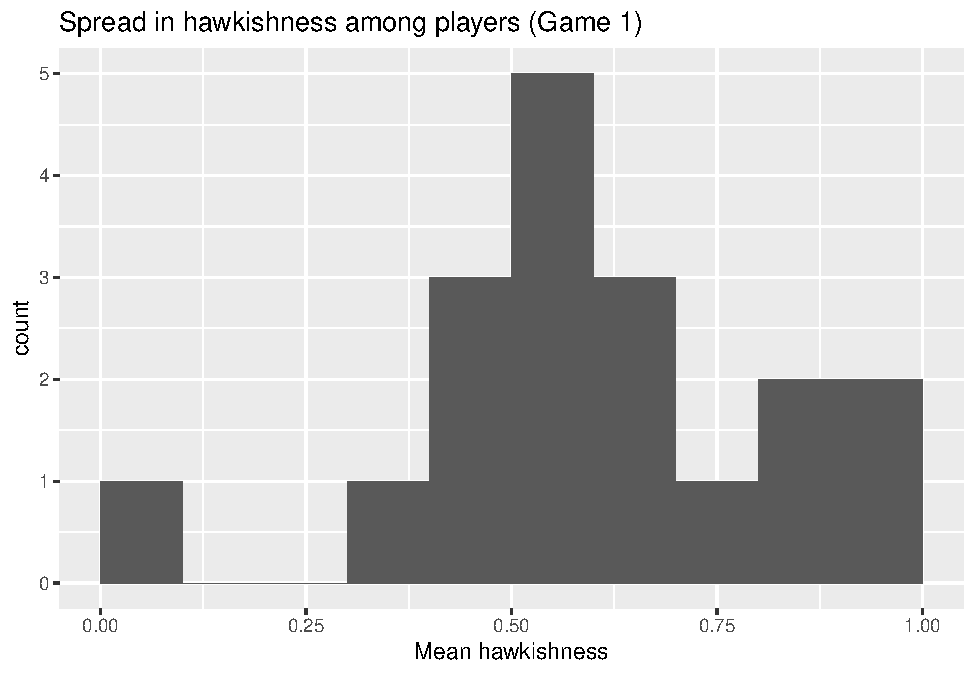
\includegraphics[keepaspectratio]{BB512_files/BB512_files/figure-latex/hawkdoveresults3-1.pdf}}

Is this more spread than we would expect by chance? The lecture showed that a mixed ESS can be reached in two ways: a mixture of pure Hawks and pure Doves, or every individual playing Hawk with the same probability. If every player had played Hawk with the same probability (0.62) in each of their 15 rounds, chance alone would give a standard deviation in hawkishness among players of about 0.13. The observed standard deviation is 0.22, so these players really did differ in strategy: some were consistently hawkish, others consistently dovish.

Did the level of hawkishness change as the game went on?

\pandocbounded{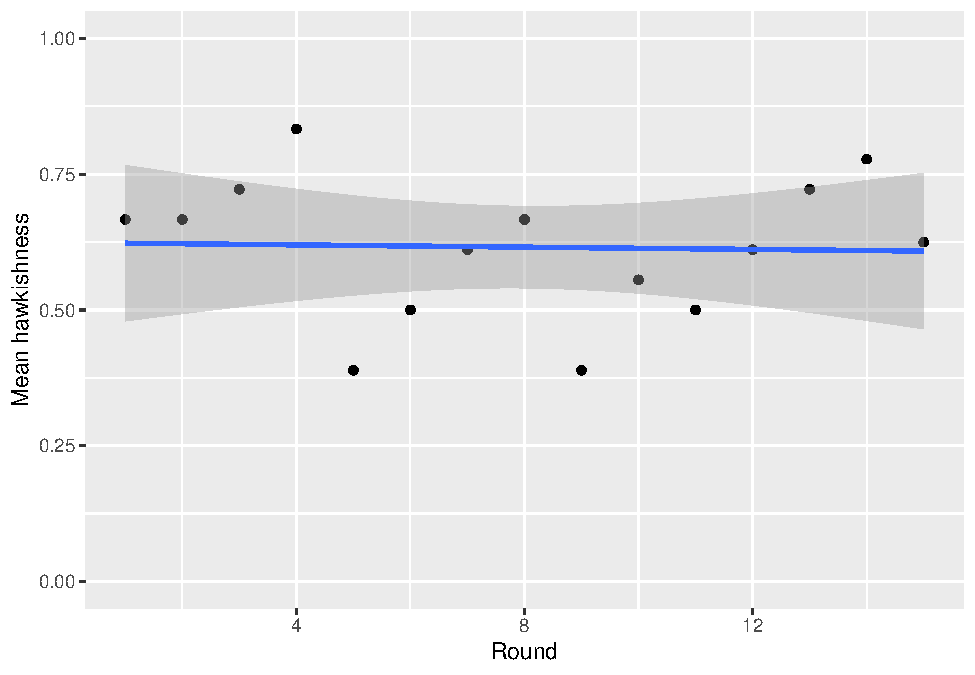
\includegraphics[keepaspectratio]{BB512_files/BB512_files/figure-latex/hawkdoveresults5-1.pdf}}

No: there is no detectable trend across the 15 rounds (p = 0.9). Nor was there a jump in Hawk play in the final round (round 15: 0.62), even though there was no next round in which to be punished.

\subsection{Does being hawkish pay with a fixed partner?}\label{does-being-hawkish-pay-with-a-fixed-partner}

With the payoffs used in this game (B = 4, C = 3), a \emph{single, anonymous} encounter has a simple answer. Because B \textgreater{} C, Hawk beats Dove regardless of what your opponent plays (Hawk-vs-Dove gives 4 \textgreater{} 2 for Dove-vs-Dove, and Hawk-vs-Hawk gives 0.5 \textgreater{} 0 for Dove-vs-Hawk), so the one-shot ESS here is pure Hawk, not an intermediate mix. (The stable mix of Hawks and Doves, with Hawk frequency p* = B/C, only arises when the cost of fighting, C, exceeds the value of the resource, B: the opposite of the situation here. With B \textgreater{} C, the payoff ranking Hawk-vs-Dove \textgreater{} Dove-vs-Dove \textgreater{} Hawk-vs-Hawk \textgreater{} Dove-vs-Hawk has the same structure as the classic Prisoner's Dilemma, with Hawk playing the role of ``Defect''.)

This has an important consequence: \textbf{within a pair, the more hawkish player always earns at least as much as their partner}, because in every round Hawk earns more than Dove against the same opponent. So asking ``who won in each pair?'' always favours Hawk. The interesting question for Game 1 is a different one: do pairs that play Hawk a lot end up worse off, \emph{both of them}, than pairs that hold back?

To answer it, we look at each pair as a unit: the pair's mean hawkishness (both players' cards) against the pair's mean payoff per player per round.

\pandocbounded{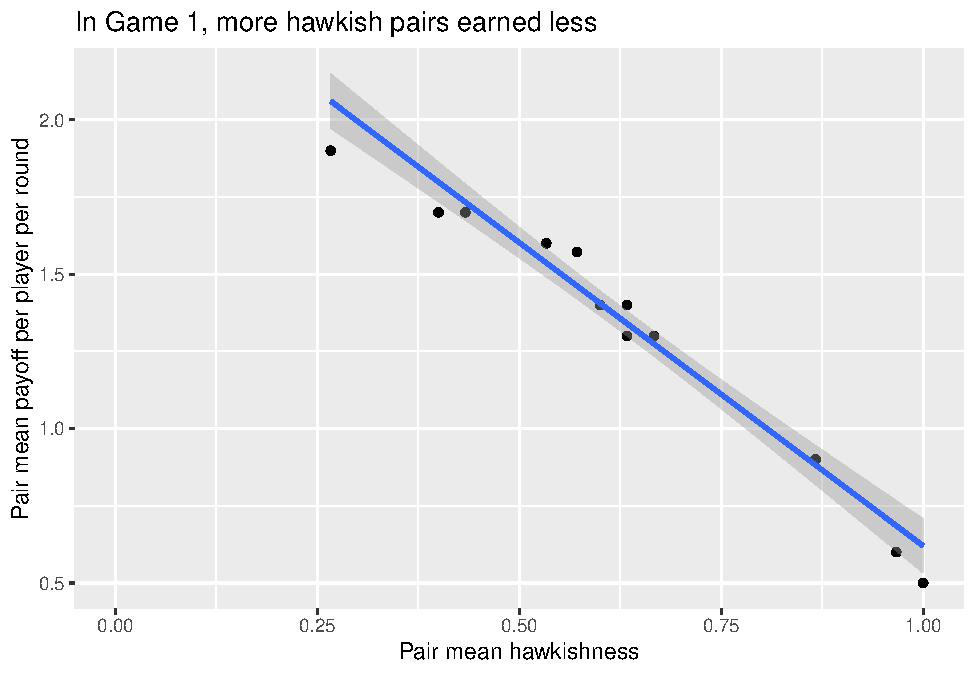
\includegraphics[keepaspectratio]{BB512_files/BB512_files/figure-latex/hawkdoveresults6-1.pdf}}

The relationship is strongly negative (slope -1.96 per round): pairs that escalated a lot got stuck in Hawk-Hawk rounds worth only 0.5 each, while pairs that held back earned close to the 2 per round of mutual Dove. (The data file records players rather than pair IDs, so most pairs appear twice in this plot, once from each partner's records, and the two points usually lie on top of each other. Because of this duplication we do not quote a p-value.)

That is the pattern expected if hawkishness provokes hawkishness: with a fixed partner, playing Hawk does not make you lose to your partner, but it lowers what \emph{both} of you earn.

\textbf{Reciprocity in repeated games}

This idea is not covered in the lecture, but it explains why repeated play can change the outcome.

When you meet the same partner again and again, what you do now affects how they treat you later. This is sometimes called the \emph{shadow of the future}. A simple strategy that does well in repeated Prisoner's Dilemma games is \textbf{tit-for-tat}: cooperate (Dove) in the first round, then copy whatever your partner did in the previous round. Tit-for-tat is never the first to escalate, punishes escalation immediately, and forgives as soon as the partner returns to Dove (Axelrod \& Hamilton 1981, \emph{Science} 211: 1390-1396).

Two caveats. First, in a game of known, fixed length, defecting (Hawk) in the last round always pays, because there is no future to protect, so cooperation is not guaranteed in theory (in practice people often cooperate anyway). Second, with the class payoffs, taking turns (Hawk/Dove, then Dove/Hawk) pays exactly as well as mutual Dove, 2 per round each, so there is more than one way to cooperate.

\section{Game 2: a new partner every round}\label{game-2-a-new-partner-every-round}

The students were asked to compete against a new opponent every round. The idea was that this would make it much harder to learn your opponent's strategy, and harder to come to an agreement that reduces aggression.

The average hawkishness in Game 2 was 0.69, a little higher than in Game 1 (0.62).

\pandocbounded{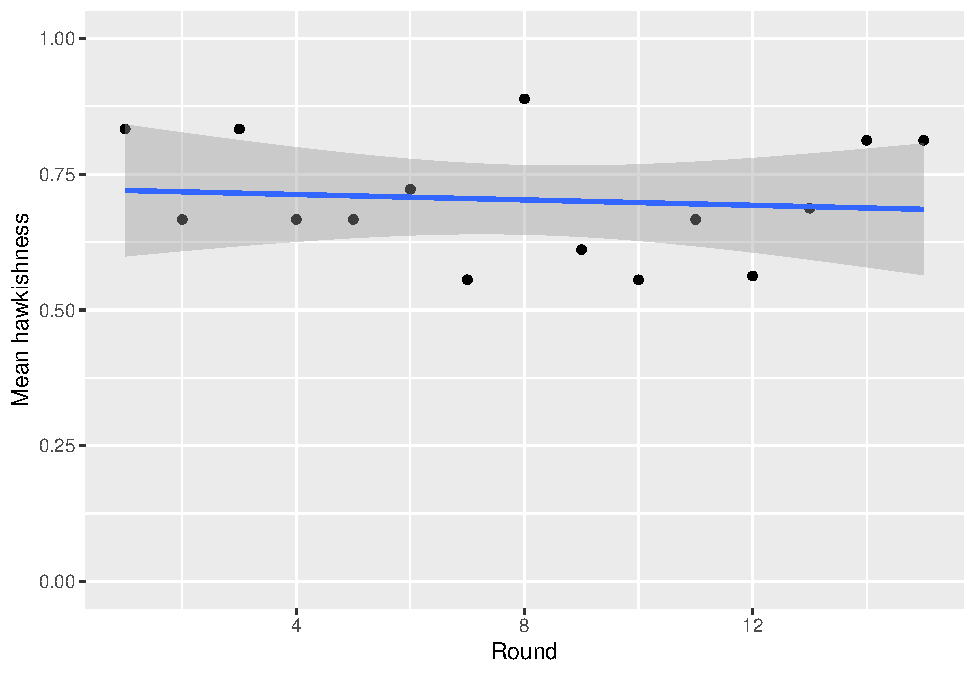
\includegraphics[keepaspectratio]{BB512_files/BB512_files/figure-latex/hawkdoveresults9-1.pdf}}

Again, hawkishness did not change systematically over the game (p = 0.72).

Finally, we can look at what the best strategy is in Game 2. Here each point is one player, and we use the mean payoff per round, because a few players missed some rounds.

\pandocbounded{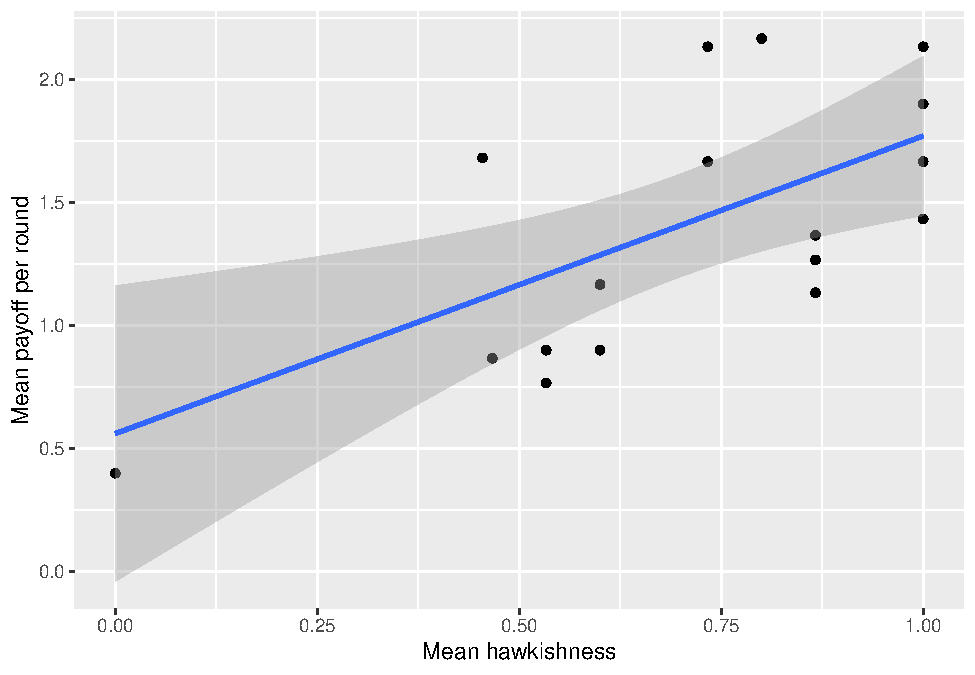
\includegraphics[keepaspectratio]{BB512_files/BB512_files/figure-latex/hawkdoveresults10-1.pdf}}

The best strategy has changed: now the more hawkish players earned more (slope 1.21 per round, p = 0.006).

This matches the one-shot theoretical prediction much better than Game 1 did. In Game 2 you faced a new partner every round, so there was no opportunity to build reciprocity, and no way to be ``punished'' for playing Hawk against the same individual again. With no repeated interaction, no ``shadow of the future'', the game reduces to the simple one-shot logic, and since B \textgreater{} C, Hawk pays off best.

In this setting we might expect natural selection to drive towards the evolution of more aggressive individuals.

\section{Comparing the two games}\label{comparing-the-two-games}

Our hypothesis was that, compared with Game 2, players in Game 1 would play Hawk less often and earn more per round. In this class, hawkishness was slightly lower in Game 1 (0.62 vs 0.69 per player; p = 0.34), but mean payoff per round was \emph{not} higher (1.25 vs 1.4; p = 0.36). Neither difference is statistically significant, so with one class of 18 players we cannot reject the null hypothesis. Remember too that Game 2 was always played after Game 1, so any difference between the games could also reflect learning or fatigue.

What did differ clearly between the games was \emph{which} strategy paid: within Game 1, pairs that held back did best, while within Game 2, individual Hawks did best.

Put together, the two games illustrate a general result from game theory: repeated interaction with the same partner can favour restraint even in a game where Hawk wins any single encounter, while anonymous, one-off interactions favour the individually dominant strategy. This is one reason why reputation, memory, and repeated encounters matter so much for the evolution of cooperation, both in nature and in human societies.

Think about what this means in terms of human cooperation and conflict avoidance.

Can you see the value of understanding your opponent/competitor?

\chapter*{Part 7: Appendix - extras}\label{part-7}
\addcontentsline{toc}{chapter}{Part 7: Appendix - extras}

\chapter{Exponential growth in detail}\label{exponential-growth-in-detail}

One of the foundational concepts in population dynamics is the exponential growth model. This model is a simplified representation of how populations grow when resources are not limiting. While it's rare for populations to experience uninhibited growth for extended periods, understanding this basic model is crucial for understanding more complex dynamics that include factors like resource limitations, predation, and disease.

In this chapter, we will explore the mathematical framework that describes exponential growth in both discrete and continuous time settings. We will introduce key parameters such as the per-capita birth rate, death rate, and intrinsic rate of increase. We will also demonstrate how to apply these models using R programming, offering a practical dimension to these theoretical concepts.

Learning outcomes:

\begin{itemize}
\tightlist
\item
  Understand the fundamental equations that underpin exponential growth in populations.
\item
  Differentiate between discrete and continuous time models.
\item
  Interpret the role and significance of various parameters in exponential growth models.
\item
  Use R programming to analyse exponential growth scenarios with real data.
\end{itemize}

\subsection{Nomenclature}\label{nomenclature}

{\def\LTcaptype{none} % do not increment counter
\begin{longtable}[]{@{}
  >{\raggedright\arraybackslash}p{(\linewidth - 4\tabcolsep) * \real{0.2571}}
  >{\raggedright\arraybackslash}p{(\linewidth - 4\tabcolsep) * \real{0.2857}}
  >{\raggedright\arraybackslash}p{(\linewidth - 4\tabcolsep) * \real{0.4571}}@{}}
\toprule\noalign{}
\begin{minipage}[b]{\linewidth}\raggedright
Symbol
\end{minipage} & \begin{minipage}[b]{\linewidth}\raggedright
Meaning
\end{minipage} & \begin{minipage}[b]{\linewidth}\raggedright
Alternatives
\end{minipage} \\
\midrule\noalign{}
\endhead
\bottomrule\noalign{}
\endlastfoot
\(R\) & Per capita rate of increase, per capita population growth rate (discrete time) & \(R_m\) (Neal), \(r_d\) (Gotelli) \\
\(r\) & Intrinsic rate of increase (continuous time) & \(r_m\) (Neal). From a life table, \(r \approx \ln(R_0)/T\), which Neal calls \(r_c\), the capacity for increase \\
\(\lambda\) & Population growth rate, population multiplication rate & \\
\(R_0\) & Net reproductive rate: the expected number of female offspring per female, per generation (\(\sum l_x m_x\)) & Not the same as the ``basic reproduction number'' of epidemiology, which uses the same symbol \\
\end{longtable}
}

\section{Discrete time model}\label{discrete-time-model}

We'll first look at \emph{discrete} population growth, which is the population growth that is considered to grow over distinct time steps (e.g., 1 year intervals). This is also called \textbf{Geometric Population Growth}.

A population at time \(t\) has size \(N\): \(N_t\).

After one time interval, there will be some births (\(B\)), and some deaths (\(D\)). Births will have the effect of increasing the population size at time \(t+1\) while deaths will decrease population size. The population at the next time step (\(N_{t+1}\)) is thus:

\textbf{eqn. 1.} \(N_{t+1} = N_t + B - D\)

We can think about the birth/death processes on a per-individual basis, and use per-capita birth rate (\(b\)) and per-capita death rate (\(d\)). We can think of \(b\) as the average number of offspring produced by an individual during the time interval starting at \(N_t\) and ending at \(N_{t+1}\). Similarly, \(d\) is the probability that an individual alive at \(N_t\) will die at some point during the interval.

The \textbf{total} number of births within a time interval depends on the number of individuals there are at the start of the interval (\(N_t\)), and the total number of births in the population during the time interval is \(bN_t\). Similarly, the total number of deaths is \(dN_t\). Thus:

\textbf{eqn. 2.} \(N_{t+1} = N_t + bN_t - dN_t\).

This equation can be simplified to:

\textbf{eqn. 3.} \(N_{t+1} = N_t + (b-d)N_t\).

Furthermore, because the expression \((b-d)\) is important, we can give it its own symbol, \(R\). \(R\) is called the \emph{per capita rate of increase} or the \emph{intrinsic rate of increase}. (Note that the nomenclature varies depending on the book/paper! In other places this is called \(r_d\), or \(R_m\)).

So we now have:

\textbf{eqn. 4.} \(N_{t+1} = N_t + RN_t\).

Or, if we are only interested in the \textbf{change} in population size:

\textbf{eqn. 5.} \(\frac{\Delta N}{\Delta t} = RN_t\).

Equation 4 can be simplified again, by factoring out the \(N_t\) on the right hand side:

\textbf{eqn. 6.} \(N_{t+1} = (R + 1)N_t\).

The quantity \((R+1)\) is given its own symbol: \(\lambda\), the \textbf{population multiplication rate} (also known as the ``finite rate of increase'').

\textbf{eqn. 7.} \(N_{t+1} = \lambda N_t\).

By rearranging this equation (eqn. 7) we can see that \(\lambda\) is simply the ratio of population size at time \(t+1\) and \(t\):

\textbf{eqn. 8.} \(\lambda = N_{t+1}/N_t\).

It follows, therefore, that when the population is neither growing nor declining (when \(N_{t+1}=N_t\)), \(\lambda = 1\) (and when \(R\) = 0).

\subsection{Calculating N for any future time point}\label{calculating-n-for-any-future-time-point}

Assuming the population growth rate remains constant, we can calculate the population at any time in the future.

As a starting point, consider equation 7: \(N_{t+1} = \lambda N_t\).

If we want to calculate \(N_{t+2}\), we would need to plug in \(N_{t+1}\) instead of \(N_t\): \(N_{t+2} = \lambda N_{t+1}\),

and, since we know that \(N_{t+1} = \lambda N_t\),: \(N_{t+2} = \lambda   \lambda N_t\).

Similarly, if we wanted to calculate \(N_{t+2}\), we'd end up with: \(N_{t+3} = \lambda \lambda \lambda N_t\).

This can be simplified by raising \(\lambda\) to a suitable power, and using the starting population at time = 0, \(N_0\):

\textbf{eqn. 9.} \(N_{t} = \lambda ^tN_0\).

This should be familiar to those of you that did (or remember!) the concept of geometric series which was covered in MM554 Mathematics for Biology.

\subsection{Applying the model}\label{applying-the-model}

If we plot exponential growth on a log scale we can see that it is straight line. For example, in the plot below I show the sequence for a population with a starting population of 1 and a \(\lambda\) (population multiplication rate) of 1.2 (i.e., the population increases by 20\% each year). In (A) the time series is plotted on the natural scale while in (B) it is plotted on the log scale.

\begin{Shaded}
\begin{Highlighting}[]
\CommentTok{\# Load required libraries}
\FunctionTok{require}\NormalTok{(tidyverse)}

\CommentTok{\# Set initial population and lambda}
\NormalTok{startPop }\OtherTok{\textless{}{-}} \DecValTok{1}
\NormalTok{lambda }\OtherTok{\textless{}{-}} \FloatTok{1.2}

\CommentTok{\# Create a data frame with time and corresponding population}
\NormalTok{df1 }\OtherTok{\textless{}{-}} \FunctionTok{data.frame}\NormalTok{(}\AttributeTok{time =} \DecValTok{0}\SpecialCharTok{:}\DecValTok{20}\NormalTok{) }\SpecialCharTok{\%\textgreater{}\%} 
  \FunctionTok{mutate}\NormalTok{(}\AttributeTok{N =}\NormalTok{ lambda}\SpecialCharTok{\^{}}\NormalTok{time }\SpecialCharTok{*}\NormalTok{ startPop)}
\end{Highlighting}
\end{Shaded}

\begin{Shaded}
\begin{Highlighting}[]
\CommentTok{\# Plotting the data}
\FunctionTok{par}\NormalTok{(}\AttributeTok{mfrow=}\FunctionTok{c}\NormalTok{(}\DecValTok{1}\NormalTok{,}\DecValTok{2}\NormalTok{))}

\CommentTok{\# Plot on natural scale}
\FunctionTok{plot}\NormalTok{(df1}\SpecialCharTok{$}\NormalTok{time, df1}\SpecialCharTok{$}\NormalTok{N, }\AttributeTok{type =} \StringTok{"b"}\NormalTok{, }\AttributeTok{xlab =} \StringTok{"time"}\NormalTok{, }\AttributeTok{ylab =} \StringTok{"N"}\NormalTok{)}
\FunctionTok{title}\NormalTok{(}\StringTok{"A"}\NormalTok{)}

\CommentTok{\# Plot on log scale}
\FunctionTok{plot}\NormalTok{(df1}\SpecialCharTok{$}\NormalTok{time, }\FunctionTok{log}\NormalTok{(df1}\SpecialCharTok{$}\NormalTok{N), }\AttributeTok{type =} \StringTok{"b"}\NormalTok{, }\AttributeTok{xlab =} \StringTok{"time"}\NormalTok{, }\AttributeTok{ylab =} \StringTok{"log(N)"}\NormalTok{)}
\FunctionTok{title}\NormalTok{(}\StringTok{"B"}\NormalTok{)}
\end{Highlighting}
\end{Shaded}

\pandocbounded{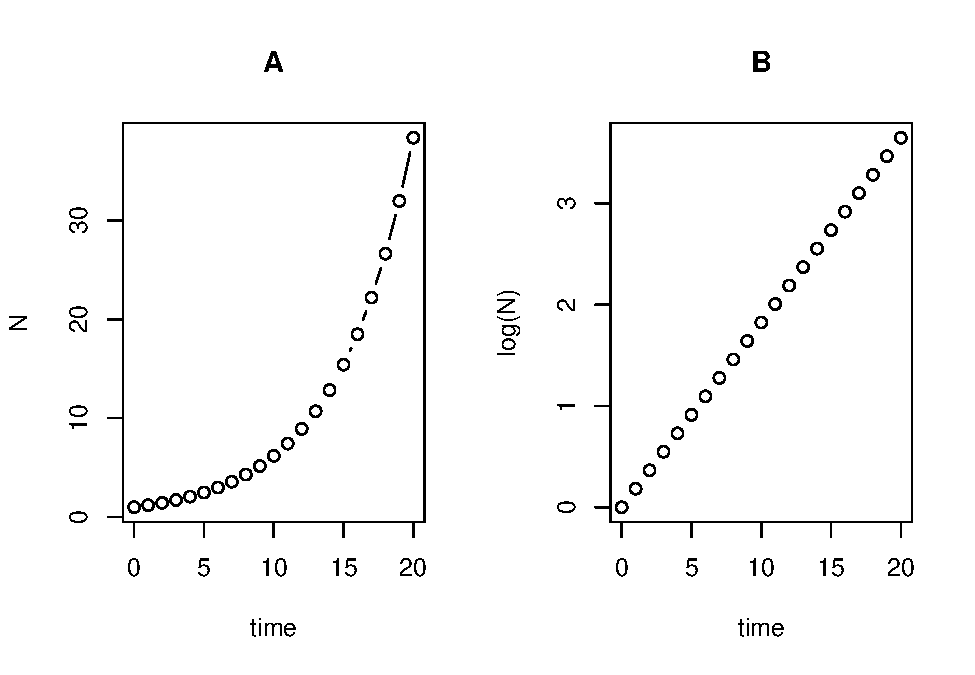
\includegraphics[keepaspectratio]{BB512_files/BB512_files/figure-latex/unnamed-chunk-44-1.pdf}}

In fact, we can linearise the relationship by log transforming both sides of equation 9:

\(\ln{N_t} = \ln(\lambda ^tN_0)\),

which can be re-written as:

\(\ln{N_t} =  \ln(\lambda )t + \ln(N_0)\).

This looks familiar. Indeed, the equation of a straight line (\(y = ax + b\)) maps onto this. In this equation, the slope \(a\) is equivalent to \(\ln(\lambda )\) and the intercept (\(b\)) is equivalent to \(\ln(N_0)\).

This is very convenient because now we can use simple regression methods to estimate \(\ln(\lambda)\) (the slope) of the relationship, and therefore the value of \(\lambda\) (or \(R\), which is \(\lambda -1\)).

\section{Real-World Application: Breeding Pairs of Merlin (Falco columbarius)}\label{real-world-application-breeding-pairs-of-merlin-falco-columbarius}

To bring these mathematical concepts to life, let's consider an example from the Neal textbook that focuses on the population of breeding pairs of Merlin, a species of small falcon. The data spans from 1970 to 1982 and shows the following population sizes (breeding pairs): \texttt{1,1,2,4,2,3,5,6,7,10,12,14,16}

This is not much data, so we can simply put it into R manually, and plot it, like this:

\begin{Shaded}
\begin{Highlighting}[]
\NormalTok{df1 }\OtherTok{\textless{}{-}} \FunctionTok{data.frame}\NormalTok{(}\AttributeTok{year =} \DecValTok{1970}\SpecialCharTok{:}\DecValTok{1982}\NormalTok{, }
                  \AttributeTok{N =} \FunctionTok{c}\NormalTok{(}\DecValTok{1}\NormalTok{,}\DecValTok{1}\NormalTok{,}\DecValTok{2}\NormalTok{,}\DecValTok{4}\NormalTok{,}\DecValTok{2}\NormalTok{,}\DecValTok{3}\NormalTok{,}\DecValTok{5}\NormalTok{,}\DecValTok{6}\NormalTok{,}\DecValTok{7}\NormalTok{,}\DecValTok{10}\NormalTok{,}\DecValTok{12}\NormalTok{,}\DecValTok{14}\NormalTok{,}\DecValTok{16}\NormalTok{))}
\FunctionTok{plot}\NormalTok{(df1}\SpecialCharTok{$}\NormalTok{year,df1}\SpecialCharTok{$}\NormalTok{N, }\AttributeTok{type =} \StringTok{"b"}\NormalTok{)}
\end{Highlighting}
\end{Shaded}

\pandocbounded{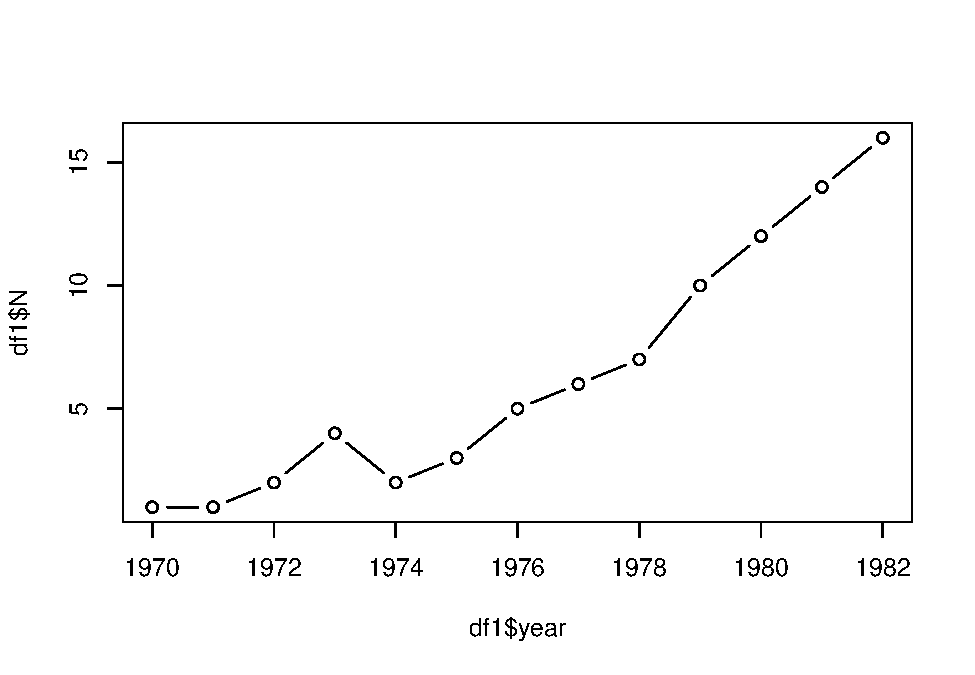
\includegraphics[keepaspectratio]{BB512_files/BB512_files/figure-latex/plotnewproj-1.pdf}}

\subsection{Observations and Context}\label{observations-and-context}

It is clear from the graph that the number of breeding pairs is increasing over the years, albeit with some fluctuations. These fluctuations could be due to various factors such as changes in food availability, predation, or human activity. However, the general trend suggests growth.

\subsection{Applying the Exponential Growth Model}\label{applying-the-exponential-growth-model}

To analyse this data, we'll use the exponential growth model. We'll plot the data on a log scale and fit a regression model:

\begin{Shaded}
\begin{Highlighting}[]
\NormalTok{df1}\SpecialCharTok{$}\NormalTok{logN }\OtherTok{\textless{}{-}} \FunctionTok{log}\NormalTok{(df1}\SpecialCharTok{$}\NormalTok{N)}
\FunctionTok{plot}\NormalTok{(df1}\SpecialCharTok{$}\NormalTok{year,df1}\SpecialCharTok{$}\NormalTok{logN)}

\NormalTok{mod1 }\OtherTok{\textless{}{-}} \FunctionTok{lm}\NormalTok{(logN}\SpecialCharTok{\textasciitilde{}}\NormalTok{year,}\AttributeTok{data =}\NormalTok{ df1)}
\FunctionTok{abline}\NormalTok{(mod1)}
\end{Highlighting}
\end{Shaded}

\pandocbounded{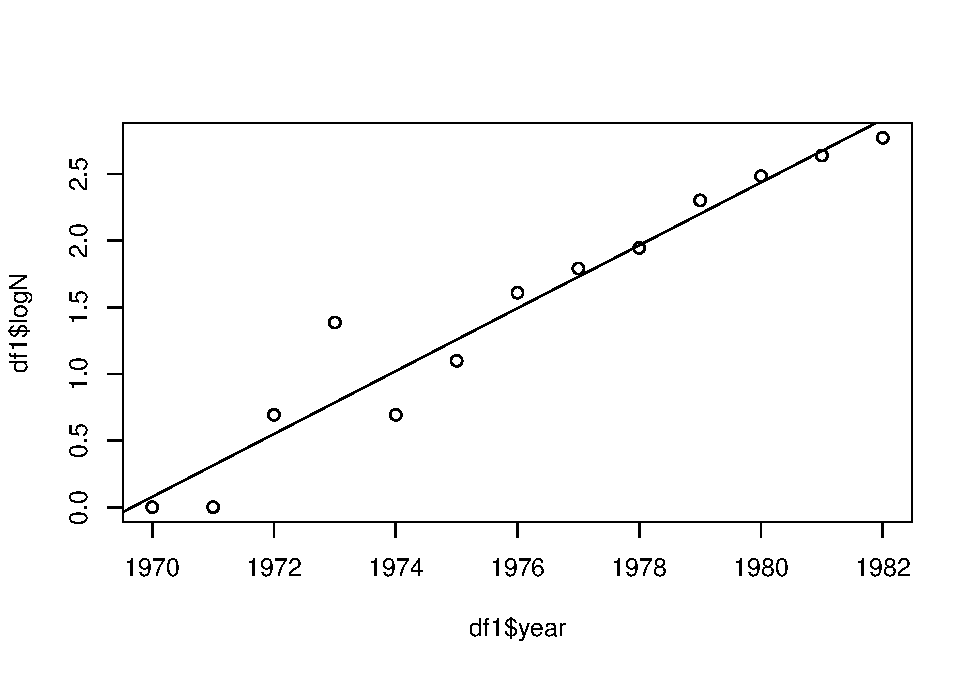
\includegraphics[keepaspectratio]{BB512_files/BB512_files/figure-latex/plotproj2-1.pdf}}

Model summary output:

\begin{verbatim}
## 
## Call:
## lm(formula = logN ~ year, data = df1)
## 
## Residuals:
##      Min       1Q   Median       3Q      Max 
## -0.32858 -0.13684 -0.01967  0.10104  0.60054 
## 
## Coefficients:
##               Estimate Std. Error t value Pr(>|t|)    
## (Intercept) -464.77072   36.12270  -12.87 5.66e-08 ***
## year           0.23596    0.01828   12.91 5.48e-08 ***
## ---
## Signif. codes:  0 '***' 0.001 '**' 0.01 '*' 0.05 '.' 0.1 ' ' 1
## 
## Residual standard error: 0.2466 on 11 degrees of freedom
## Multiple R-squared:  0.9381, Adjusted R-squared:  0.9324 
## F-statistic: 166.6 on 1 and 11 DF,  p-value: 5.478e-08
\end{verbatim}

Interpretation

The summary of the model indicates that the slope of the relationship between year and logN is 0.2359637. This slope is \(\ln(\lambda)\), so the population multiplication rate (\(\lambda\)) is \(e^{\text{slope}}\) = 1.266, the intrinsic rate of increase (\(r\)) is the slope itself = 0.236, and the per capita rate of increase (\(R = \lambda - 1\)) is 0.266.

This suggests that the number of breeding pairs is indeed growing exponentially over the time period studied, with a specific rate of increase. Understanding this rate is crucial for conservation efforts, because it provides insights into the population's resilience, its demands on the ecosystem, and how it might respond to future changes in environmental conditions or conservation policies.

\section{Continuous time model}\label{continuous-time-model}

In contrast to the discrete time model, the continuous time model allows us to understand population growth without the constraint of clear time intervals. This is particularly useful for studying populations that don't have breeding seasons or for those that experience continuous births and deaths (e.g.~bacteria, humans).

The starting point for the continuous time model is the intrinsic rate of increase, \(r\). This is defined as: \(r = ln(\lambda)\) which is the same as saying \(r = ln(N_{t+1}/N_t)\)

We say that \(r = ln(\lambda)\) ``r is the natural log of lambda''.

Here, \(\lambda\) is the population multiplication rate, as discussed in the discrete time model section. The natural logarithm of \(\lambda\) gives us \(r\), which can be interpreted as the rate of population growth per unit time when resources are unlimited.

To back-transform from a natural log, we use the exponential. Therefore, \(\lambda = e^r\): ``lambda is the exponential of r''.

This allows us to relate \(\lambda\) and \(r\) directly. From the discrete model (above), we know that \(\lambda = 1 + R\), so:

\(1+R = e^r\)

\(R = e^r - 1\)

\subsection{Zero population growth}\label{zero-population-growth}

When the population is steady with zero growth, \(r = 0\) and \(\lambda  = 1\). It's important to note that the relationship \(\lambda = r + 1\) only holds true when the population is not growing or shrinking. This is a special case and should not be generalised. Do not make the common mistake to think that \(\lambda\) is simply \(r + 1\)!

\chapter{The legend of Ambalappuzha}\label{the-legend-of-ambalappuzha}

Exponential growth is a powerful concept. To help us grasp it better let's use an ancient Indian chess legend as an example.

\textbf{Learning outcomes}

\begin{itemize}
\tightlist
\item
  Use of Excel formulae for mathematical modelling.
\item
  Understanding the multiplicative process of exponential/geometric growth.
\end{itemize}

\begin{center}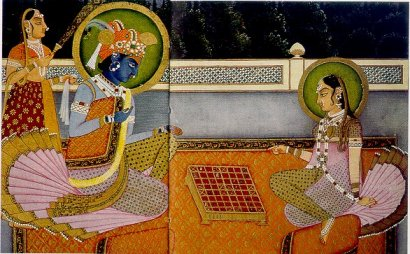
\includegraphics[width=0.5\linewidth]{images/Radha-Krishna_chess} \end{center}

According to legend, Lord Krishna once appeared in the form of a wise man in the court of the king and challenged him to a game of chess. The king was a chess enthusiast and naturally accepted the invitation.

The king asked the wise man to choose a prize in case he won. The old man told the king that he had few material needs and that all he wished was a few grains of rice.

He added that the amount of rice itself should be determined using the chessboard in the following manner: one grain of rice would be placed in the first square, two grains in the second square, four in the third square, and so on. Every square would have double the number of grains of its predecessor.

Upon hearing this, the king was unhappy, since the man requested only a few grains of rice instead of any of the other riches of the kingdom, which the king would have been happy to donate (he was a generous guy). He requested the old man to add other items to his prize, but the man declined.

So the game of chess started and, needless to say, the king lost the game so it was soon time to pay the old man his prize. As he started adding grains of rice to the chessboard, the king soon realised the true nature of the wise man's demand. The royal granary soon ran out of rice and the king realised that even if he provided all the rice in his kingdom and even the whole of India, he would never be able to fulfil the promised reward. He was distraught that he could not fulfil his promise!

Seeing the king upset, the wise man appeared to the king in his true form, that of Lord Krishna. He told the king that he did not have to pay the debt immediately but could pay him over time. The king would serve rice in the temple freely to the pilgrims every day until the debt was paid off. And that is why the Ambalappuzha Temple in India still serves rice pudding (palpayasam) to pilgrims -- the debt is still being paid off.

Use the Excel sheet \href{https://www.dropbox.com/s/nf81t0hzz34vyzk/RiceOnAChessboard.xlsx?dl=1}{RiceOnAChessboard.xlsx} to calculate the quantity of rice that the king owed.

A grain of rice weighs 25mg, what weight of rice did the king owe in total, in kg?

\section{Animals/plants, not grains of rice}\label{animalsplants-not-grains-of-rice}

Imagine that instead of rice, we were talking about population growth---e.g.~bacteria or rabbits---reproducing every time-step.

\subsection{Quick exercise (optional)}\label{quick-exercise-optional}

We have \textasciitilde100 breeding pairs of great tits (musvit) in woodland around SDU. Each female lays \textasciitilde6 eggs per year with an assumed 50:50 sex ratio.

\begin{itemize}
\tightlist
\item
  \textbf{If survival were 100\%}, how many females would there be after 5 years?
\item
  \textbf{Now relax that assumption:} allow realistic survival and recruitment. How do your answers change?
\end{itemize}

\subsection{Discussion prompts}\label{discussion-prompts}

\begin{itemize}
\tightlist
\item
  \textbf{Is the simple doubling model realistic?}

  \begin{itemize}
  \tightlist
  \item
    Why / why not?
  \end{itemize}
\item
  \textbf{Key processes to consider:}

  \begin{itemize}
  \tightlist
  \item
    Survival \textless{} 100\%; age/stage-specific survival and fecundity
  \item
    Density dependence (resources, territories, disease, predation)
  \item
    Carrying capacity and feedbacks on reproduction/survival
  \end{itemize}
\item
  \textbf{Variation over time and space:}

  \begin{itemize}
  \tightlist
  \item
    Stochasticity (good/bad years), seasonality, environmental drivers
  \item
    Dispersal, immigration/emigration
  \end{itemize}
\item
  \textbf{Model structure:}

  \begin{itemize}
  \tightlist
  \item
    Age/stage structure (e.g.~juvenile vs adult), sex ratio, mating system
  \item
    Time-step choice (daily/weekly/annual) and what processes occur within a step
  \end{itemize}
\end{itemize}

\section{Optional: Try these calculations in R}\label{optional-try-these-calculations-in-r}

You can do this kind of calculation easily in \emph{R}. Try this.

\begin{Shaded}
\begin{Highlighting}[]
\NormalTok{myData }\OtherTok{\textless{}{-}} \FunctionTok{data.frame}\NormalTok{(}\AttributeTok{Squares =} \DecValTok{1}\SpecialCharTok{:}\DecValTok{64}\NormalTok{,}\AttributeTok{nRice =} \ConstantTok{NA}\NormalTok{)}
\NormalTok{myData}\SpecialCharTok{$}\NormalTok{nRice[}\DecValTok{1}\NormalTok{] }\OtherTok{\textless{}{-}} \DecValTok{1} 

\ControlFlowTok{for}\NormalTok{ (i }\ControlFlowTok{in} \DecValTok{2}\SpecialCharTok{:}\DecValTok{64}\NormalTok{)\{}
\NormalTok{  myData}\SpecialCharTok{$}\NormalTok{nRice[i] }\OtherTok{\textless{}{-}}\NormalTok{ myData}\SpecialCharTok{$}\NormalTok{nRice[i}\DecValTok{{-}1}\NormalTok{]}\SpecialCharTok{*}\DecValTok{2}
\NormalTok{\}}
\end{Highlighting}
\end{Shaded}

Now we can look at the top and bottom of the 64 row data frame like this:

\begin{Shaded}
\begin{Highlighting}[]
\FunctionTok{head}\NormalTok{(myData)}
\end{Highlighting}
\end{Shaded}

\begin{verbatim}
##   Squares nRice
## 1       1     1
## 2       2     2
## 3       3     4
## 4       4     8
## 5       5    16
## 6       6    32
\end{verbatim}

\begin{Shaded}
\begin{Highlighting}[]
\FunctionTok{tail}\NormalTok{(myData)}
\end{Highlighting}
\end{Shaded}

\begin{verbatim}
##    Squares        nRice
## 59      59 2.882304e+17
## 60      60 5.764608e+17
## 61      61 1.152922e+18
## 62      62 2.305843e+18
## 63      63 4.611686e+18
## 64      64 9.223372e+18
\end{verbatim}

Output preview:

\begin{verbatim}
##   Squares nRice
## 1       1     1
## 2       2     2
## 3       3     4
## 4       4     8
## 5       5    16
## 6       6    32
\end{verbatim}

\begin{verbatim}
##    Squares        nRice
## 59      59 2.882304e+17
## 60      60 5.764608e+17
## 61      61 1.152922e+18
## 62      62 2.305843e+18
## 63      63 4.611686e+18
## 64      64 9.223372e+18
\end{verbatim}

And we can sum up the total number of grains of rice on the 64 squares of the board like this:

\begin{Shaded}
\begin{Highlighting}[]
\FunctionTok{sum}\NormalTok{(myData}\SpecialCharTok{$}\NormalTok{nRice)}
\end{Highlighting}
\end{Shaded}

\begin{verbatim}
## [1] 1.844674e+19
\end{verbatim}

Output:

\begin{verbatim}
## [1] 1.844674e+19
\end{verbatim}

To put that \emph{HUGE} number in context, if a grain of rice weighs 25mg (0.000025kg), then we'd have 461,168,601,842,739 kg. That's 461 Gigatonnes, or roughly 8-900 times the yearly global rice production!

\chapter{From population biology to fitness}\label{from-population-biology-to-fitness}

The purpose of this practical is to draw clear links between the first part of the course (population biology) and the second part of the course (evolution).

Learning outcomes:

\begin{itemize}
\tightlist
\item
  Understanding the relationship between population growth and the concept of fitness.
\item
  Understanding the concept of an evolutionary trade-off.
\end{itemize}

We will focus on the concept of \textbf{fitness}.

Fitness is a slippery concept, but it is widely accepted that it is closely related to population growth rate. In this class you will explore this concept using some mathematical modelling.

This practical uses RStudio (R). It is similar to the previous exercise on matrix population models, but ask for help if you get stuck!

\section{\texorpdfstring{An \emph{in silico} experiment}{An in silico experiment}}\label{an-in-silico-experiment}

As you learned in the classes on age- and stage-structured population dynamics, differences in survival and reproduction can be modelled using matrix population models (MPMs). These models can be simple or complex, and can be thought of as mathematical descriptions of the life history of the species (or population) in a particular environment.

Earlier in the course you will have played with construction and analyses of these models by creating MPMs for species with different life histories such as high juvenile survival, or low juvenile survival etc.

We will first need to load the \texttt{popdemo} package like this. Note that if you have not installed this package you should first install it with the command \texttt{install.packages("popdemo")}.

Let's set up our baseline model. This model describes a population of some mammal species which we have divided into 3 stages: juvenile, adult and senescent (old).

You can ``read'' the matrix by looking at the columns and rows: a value in the column \textbf{3} and row \textbf{1} tells you the ``transition'' \textbf{from} stage 3 \textbf{to} stage 1. In this case, it is saying that an individual in the adult age class produces an average of 4 babies, and one from the senescent age class produces 2 babies. Juveniles have a probability of 0.1 (10\% chance) to survive to adulthood (and they reach maturity in 1 year, so there is no ``stasis'' where they can remain being juveniles). Adults can survive in 2 ways, they can survive and remain as adults (probability = 0.8) or they can survive and transition to being in the senescent age class (probability = 0.1). Therefore, the total survival probability is 0.9. Senescent adults survive less well (probability = 0.4).

We can project a population like this:

Take a look at \texttt{pr}, the projected population. This gives you the total population size, and below that the population sizes in each stage.

\begin{verbatim}
## 1 deterministic population projection over 8 time intervals.
## 
## [1] 18.00000 32.70000 31.18000 37.51200 42.93080 50.15272 58.36605 68.04116
## [9] 79.29730
\end{verbatim}

You can access the population sizes of the different stages using \texttt{vec(pr)}.

\begin{verbatim}
##             S1       S2       S3
##  [1,] 10.00000  5.00000 3.000000
##  [2,] 26.00000  5.00000 1.700000
##  [3,] 23.40000  6.60000 1.180000
##  [4,] 28.76000  7.62000 1.132000
##  [5,] 32.74400  8.97200 1.214800
##  [6,] 38.31760 10.45200 1.383120
##  [7,] 44.57424 12.19336 1.598448
##  [8,] 51.97034 14.21211 1.858715
##  [9,] 60.56588 16.56672 2.164697
\end{verbatim}

Let's plot this\ldots{} Check out how, after a ``transient'' period, there is exponential growth in all stages of the population. The population is growing steadily with a fixed population growth rate (\(\lambda\)).

\pandocbounded{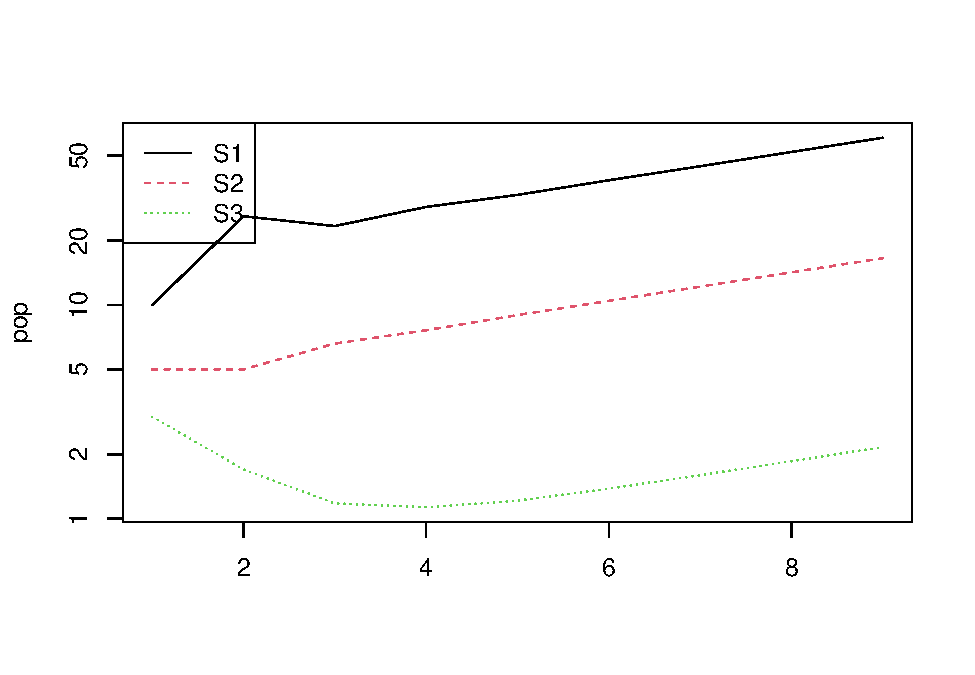
\includegraphics[keepaspectratio]{BB512_files/BB512_files/figure-latex/unnamed-chunk-56-1.pdf}}

You can see that the population is increasing and we can calculate the precise population growth rate (\(\lambda\)) like this:

\begin{verbatim}
## [1] 1.165587
\end{verbatim}

Thus, the population is growing at 16.56\% per year.

So where does evolution come in?

\section{The link to fitness}\label{the-link-to-fitness}

In this population consider that suddenly a mutation arises in an individual parent that causes it to give more care to their offspring. For example, maybe they provide milk with a higher fat content, or build a safer nest. Whatever the mechanism, let's assume that it results in a small increase in juvenile survival.

We can simulate this by increasing the juvenile survival in the matrix model from 0.10 to 0.11.

What effect does that have on population growth rate?

\begin{verbatim}
## [1] 1.192317
\end{verbatim}

The small increase in juvenile survival has resulted in a small increase in population growth rate, from 16.56\% to 19.23\% per year.

If you consider that the original population now consists of two genotypes -- ``ordinary'' and ``caring'' -- what do you think will happen to the percentage of the two genotypes through time?

You can be sure that the proportion of the caring genotype will grow faster than the ordinary genotype. It is the FITTER genotype.

\section{Introducing a trade-off}\label{introducing-a-trade-off}

It is common that apparently beneficial behaviours or innovations come at a cost. In evolutionary biology these are called \textbf{trade-offs}.

Let's explore such a trade-off now and see how it might affect fitness.

We'll stick with the same example above, but we'll introduce a new genotype that has a trade-off between juvenile survival and old-adult survival.

The benefit is clear: a change in adult behaviour or physiology increases juvenile survival a little bit.
But such changes often come with a cost: The new genotype allocates extra resources to babies but this exhausts the adults causing older adults to have very small survival probability.

Is this new genotype viable? In other words, is the fitness of the genotype greater than that of the original genotype? If so, the new genotype will come to dominate the population.

Modify the matrix to reduce old adult survival to, say 0.05 (5\% survival) and re-calculate the population growth rate.

Is this ``trade-off genotype'' fitter than the original one? i.e.~is the small benefit worth the large cost?

Try doing the same thing for the prime-age adults. How much can you reduce survival before the cost is not worth bearing?

\chapter{From plain English to a matrix model}\label{from-plain-english-to-a-matrix-model}

\section{Background}\label{background-19}

This activity is designed for quick in-class practice translating a verbal life-history description into a matrix population model. It connects directly to the workflow in \texttt{2\_07\_matrixModels.Rmd}.

Learning outcomes:

\begin{itemize}
\tightlist
\item
  Convert a verbal life-history description into a matrix population model.
\item
  Build and interpret a simple projection from initial stage abundances.
\end{itemize}

\section{Worked example}\label{worked-example-9}

\subsection{Inputs}\label{inputs-7}

Suppose juveniles do not reproduce, each adult contributes 2 offspring per year that survive to be counted as juveniles at the next census, juvenile survival is 0.4, and adult survival is 0.7. A simple stage matrix would be:

\subsection{Steps}\label{steps-7}

\begin{enumerate}
\def\labelenumi{\arabic{enumi}.}
\tightlist
\item
  Put fecundity terms in the top row (when all newborns enter stage 1). A fecundity term is the number of offspring counted at the \emph{next} census per individual now, so it must include any survival needed to get there (see the fecundity box in the chapter ``Matrix population modelling''). If a description gives you the number of babies born, multiply by the survival needed to reach the next count.
\item
  Put survival/transition terms in the subdiagonal/diagonal entries.
\item
  Assemble the matrix in row = stage at \(t+1\), column = stage at \(t\) form.
\end{enumerate}

\subsection{Output and interpretation}\label{output-and-interpretation-7}

\[
A =
\begin{bmatrix}
0 & 2 \\
0.4 & 0.7
\end{bmatrix}
\]

The key idea is to map each biological statement to a matrix entry: fecundity goes in the top row, survival and stage transitions go on the sub-diagonal or main diagonal.

\section{Your task}\label{your-task-21}

Use the red-tailed hawk life history description in \texttt{supplemental/Exercise\_Plain\_English\_To\_Matrix\_Model\_2018.txt}.

\begin{enumerate}
\def\labelenumi{\arabic{enumi}.}
\tightlist
\item
  Draw a 3-stage life cycle diagram (hatchling, juvenile, adult).
\item
  Translate the verbal description into a 3x3 projection matrix. State any assumptions you make about the juvenile stasis and transition rates.
\item
  Use the initial population sizes given (1000 hatchlings, 150 juveniles, 5 adults) and project the population for 20 time steps.
\item
  Calculate the dominant eigenvalue and interpret whether the population grows or declines.
\item
  Compare your approach with the workflow in \texttt{2\_07\_matrixModels.Rmd}.
\end{enumerate}

\section{Takeaways}\label{takeaways-22}

\begin{itemize}
\tightlist
\item
  Verbal life-history descriptions can be translated directly into matrix entries with clear assumptions.
\item
  Simple projections reveal whether the implied population is growing or declining.
\end{itemize}

\chapter{Continuous traits from discrete genes}\label{continuous-traits-from-discrete-genes}

\section{Background}\label{background-20}

This activity uses a fast classroom simulation to show how many small genetic effects can generate a continuous, approximately normal trait distribution. It connects to the heritability workflow in \texttt{3\_04\_Heritability.Rmd}.

Learning outcomes:

\begin{itemize}
\tightlist
\item
  Explain how additive genetic effects create continuous trait variation.
\item
  Compare a classroom simulation with a simple R simulation.
\end{itemize}

\section{Worked example}\label{worked-example-10}

\subsection{Inputs}\label{inputs-8}

\begin{itemize}
\tightlist
\item
  Baseline trait value: \texttt{35}
\item
  Number of genes: \texttt{25}
\item
  Each gene contributes \texttt{1} unit when ON
\end{itemize}

\subsection{Steps}\label{steps-8}

\begin{enumerate}
\def\labelenumi{\arabic{enumi}.}
\tightlist
\item
  Compute expected number of ON genes under 50:50 ON/OFF: \texttt{25\ *\ 0.5\ =\ 12.5}.
\item
  Add expected genetic contribution to baseline.
\end{enumerate}

\subsection{Output and interpretation}\label{output-and-interpretation-8}

Expected trait value is \texttt{35\ +\ 12.5\ =\ 47.5}. Individual values vary around this because each gene is ON or OFF stochastically.

\section{Your task}\label{your-task-22}

Use the intuition exercise in \texttt{supplemental/Quantitative\_Genetics/Continuous\_Traits\_From\_Discrete\_Genes.docx} and the spreadsheet in \texttt{supplemental/Quantitative\_Genetics/Continuous\_Traits\_From\_Discrete\_Genes.xlsx}.

\begin{enumerate}
\def\labelenumi{\arabic{enumi}.}
\tightlist
\item
  In class, treat each student as a gene that can be ON (1) or OFF (0). Choose a baseline trait value of 35, and add 1 for each ON gene. Record the trait value for at least 30 individuals.
\item
  Plot a quick histogram of the observed trait values. Describe the shape.
\item
  Now simulate the same process in R for 100 individuals and 25 genes. Compare your histogram to the classroom version.
\item
  Relate the outcome to the concept of additive genetic variance in \texttt{3\_04\_Heritability.Rmd}.
\end{enumerate}

\begin{Shaded}
\begin{Highlighting}[]
\NormalTok{baseline }\OtherTok{\textless{}{-}} \DecValTok{35}
\NormalTok{n\_genes }\OtherTok{\textless{}{-}} \DecValTok{25}
\NormalTok{n\_individuals }\OtherTok{\textless{}{-}} \DecValTok{100}

\NormalTok{gene\_on }\OtherTok{\textless{}{-}} \FunctionTok{rbinom}\NormalTok{(n\_individuals, }\AttributeTok{size =}\NormalTok{ n\_genes, }\AttributeTok{prob =} \FloatTok{0.5}\NormalTok{)}
\NormalTok{trait\_value }\OtherTok{\textless{}{-}}\NormalTok{ baseline }\SpecialCharTok{+}\NormalTok{ gene\_on}

\FunctionTok{hist}\NormalTok{(trait\_value, }\AttributeTok{breaks =} \DecValTok{12}\NormalTok{, }\AttributeTok{col =} \StringTok{"gray80"}\NormalTok{, }\AttributeTok{main =} \StringTok{"Trait values"}\NormalTok{, }\AttributeTok{xlab =} \StringTok{"Trait"}\NormalTok{)}
\end{Highlighting}
\end{Shaded}

\pandocbounded{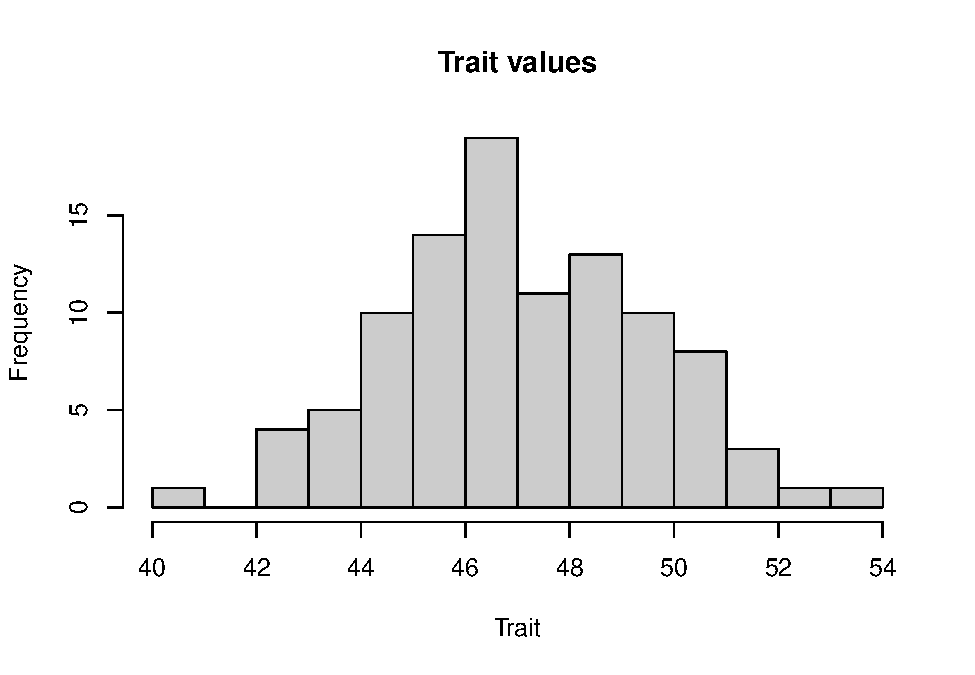
\includegraphics[keepaspectratio]{BB512_files/BB512_files/figure-latex/discrete-genes-sim-1.pdf}}

\section{Takeaways}\label{takeaways-23}

\begin{itemize}
\tightlist
\item
  Many small additive effects naturally yield a continuous distribution.
\item
  Random genetic variation produces a spread of trait values even with identical environments.
\end{itemize}

\chapter{Building a phylogenetic tree}\label{building-a-phylogenetic-tree}

\section{Background}\label{background-21}

This activity builds intuition for phylogenetic trees by using discrete morphological characters. It aligns with the macroevolution exercise guide in \texttt{supplemental/Macroevolution\_Building\_A\_Tree/FylTree\_ENG\_2015.pdf}.

Learning outcomes:

\begin{itemize}
\tightlist
\item
  Build a simple character table for a set of organisms.
\item
  Compute pairwise differences and translate them into a tree.
\item
  Relate morphology-based trees to the idea of evolutionary relatedness.
\end{itemize}

\section{Key idea}\label{key-idea-4}

With six organisms and seven characters, you can compute a pairwise difference table, then group the closest relatives first. The internal nodes represent the most recent common ancestors inferred from shared characters.

\section{Your task}\label{your-task-23}

Use \texttt{supplemental/Macroevolution\_Building\_A\_Tree/FylTree\_ENG\_2015.pdf} as a guide for the classroom activity.

\begin{enumerate}
\def\labelenumi{\arabic{enumi}.}
\tightlist
\item
  Pick six organisms (use the cards if you have them, or invent six organisms with clear traits).
\item
  Identify seven discrete characters that differ among the organisms (presence/absence, color class, tail length category, etc.).
\item
  Fill in a character table and then compute a pairwise difference table.
\item
  Draw a phylogenetic tree by grouping the closest relatives first, then adding deeper splits.
\item
  Optional: compare your hand-drawn tree with an R clustering result.
\end{enumerate}

\begin{Shaded}
\begin{Highlighting}[]
\CommentTok{\# Replace this with your own character table}
\NormalTok{characters }\OtherTok{\textless{}{-}} \FunctionTok{data.frame}\NormalTok{(}
  \AttributeTok{row.names =} \FunctionTok{c}\NormalTok{(}\StringTok{"A"}\NormalTok{, }\StringTok{"B"}\NormalTok{, }\StringTok{"C"}\NormalTok{, }\StringTok{"D"}\NormalTok{, }\StringTok{"E"}\NormalTok{, }\StringTok{"F"}\NormalTok{),}
  \AttributeTok{trait1 =} \FunctionTok{c}\NormalTok{(}\DecValTok{1}\NormalTok{, }\DecValTok{1}\NormalTok{, }\DecValTok{0}\NormalTok{, }\DecValTok{0}\NormalTok{, }\DecValTok{0}\NormalTok{, }\DecValTok{1}\NormalTok{),}
  \AttributeTok{trait2 =} \FunctionTok{c}\NormalTok{(}\DecValTok{0}\NormalTok{, }\DecValTok{1}\NormalTok{, }\DecValTok{1}\NormalTok{, }\DecValTok{0}\NormalTok{, }\DecValTok{0}\NormalTok{, }\DecValTok{1}\NormalTok{),}
  \AttributeTok{trait3 =} \FunctionTok{c}\NormalTok{(}\DecValTok{1}\NormalTok{, }\DecValTok{1}\NormalTok{, }\DecValTok{1}\NormalTok{, }\DecValTok{0}\NormalTok{, }\DecValTok{0}\NormalTok{, }\DecValTok{0}\NormalTok{)}
\NormalTok{)}

\NormalTok{dist\_mat }\OtherTok{\textless{}{-}} \FunctionTok{dist}\NormalTok{(characters, }\AttributeTok{method =} \StringTok{"manhattan"}\NormalTok{)}
\NormalTok{tree }\OtherTok{\textless{}{-}} \FunctionTok{hclust}\NormalTok{(dist\_mat, }\AttributeTok{method =} \StringTok{"average"}\NormalTok{)}
\FunctionTok{plot}\NormalTok{(tree, }\AttributeTok{main =} \StringTok{"Tree from morphological characters"}\NormalTok{)}
\end{Highlighting}
\end{Shaded}

\section{Takeaways}\label{takeaways-24}

\begin{itemize}
\tightlist
\item
  Morphological characters can be converted into a simple distance matrix.
\item
  The closest pairs in the distance matrix define the earliest groupings in a tree.
\end{itemize}

\bibliography{book.bib,packages.bib}

\end{document}
